\documentclass[12pt, a4paper, twoside, english, final]{ETHthesis}
\emergencystretch=1em
% !TEX root = thesis-index.tex
\usepackage{ETHthesis}
\usepackage[english]{babel}

% Fonts
\usepackage[OT1]{fontenc}
\usepackage[utf8]{inputenc}
\usepackage{lmodern}

% \usepackage[showframe]{geometry} # Useful to check hbox issues
\usepackage{amsmath, amssymb, amsthm}
\usepackage[dvipsnames]{xcolor}

% Biblio
\usepackage{csquotes}
\usepackage[backend=bibtex, style=alphabetic, natbib=true,
            isbn=false, backref=true, maxcitenames=3,
            maxbibnames=100]{biblatex}



% \usepackage{subcaption}
\usepackage{tikz}
\usepackage{bbm}
\usepackage{dsfont}
\usepackage{mathtools}
\usepackage{graphicx}

% Tables
\usepackage{tabularx}
\usepackage{booktabs}

% Algorithms
\usepackage{algorithm}
\usepackage[noend]{algorithmic}
\renewcommand\algorithmicthen{}
\renewcommand\algorithmicdo{}
\usepackage{eqparbox}
\renewcommand\algorithmiccomment[1]{%
  \hfill\#\ \eqparbox{COMMENT}{\textit{#1}}%
}
\usepackage{xspace}

\usepackage{enumitem}
\setlist[enumerate]{leftmargin=*}

\usepackage{titlesec}
% \usepackage{hyperref}
\usepackage[hidelinks]{hyperref}
\hypersetup{pdfauthor={Francesco Locatello}, pdftitle={}, pdfsubject={A thesis submitted to attain the degree of Doctor of Sciences to ETH Zurich},
            pdflang={en}, bookmarksnumbered, pageanchor=true, plainpages=false, colorlinks=true, linktocpage=true,
            citecolor=MidnightBlue, filecolor=BrickRed, linkcolor=NavyBlue, urlcolor=ForestGreen}

\definecolor{light-gray}{gray}{0.65}
\titleformat{\chapter}% Command
[display]% shape
{\bfseries\Large}% Format for the whole title
{\filleft{\fontsize{80}{100}\selectfont\color{light-gray}\thechapter}}% Label
{-25pt}% horizontal separation (vertical for display)
{\filleft\fontsize{26}{35}\selectfont}% Before Code
[\vspace{5pt}\titlerule]

%% Page Layout
\setlength{\topmargin}{-7.5mm}
\setlength{\headheight}{5mm}
\setlength{\headsep}{+12.5mm}
\setlength{\textheight}{220mm}
\setlength{\footskip}{+20.mm}
\setlength{\textwidth}{161mm} %!!!
\setlength{\parindent}{0pt}
\setlength{\parskip}{1ex plus 0.25ex minus 0.25ex}
\iftwoside
\setlength{\oddsidemargin}{3mm}
\setlength{\evensidemargin}{-3mm}
\else
\setlength{\oddsidemargin}{0mm}
\setlength{\evensidemargin}{0mm}
\fi
\raggedbottom

%% Float Placement
\renewcommand{\floatpagefraction}{0.9}
\renewcommand{\topfraction}{0.9}
\renewcommand{\bottomfraction}{0.9}
\renewcommand{\textfraction}{0.1}
\renewcommand{\baselinestretch}{1.15}

% Allow subsubsections to have numbers (and be references)
\setcounter{secnumdepth}{3}
% Allow subsubsections to appear in the TOC
\setcounter{tocdepth}{3}
% \setcounter{lofdepth}{2} % we want subfigures in the list of figures

%% Line spacing
\linespread{1.25}

%% Avoid Widows and Orphans
\widowpenalty=1000
\clubpenalty=1000

\vfuzz2pt % Don't report over-full v-boxes if over-edge is small
\hfuzz2pt % Don't report over-full h-boxes if over-edge is smallq

% !TEX root = thesis-index.tex
% Allow overfull boxes which don't overflow more than 20pts (remove before the last version)
\hfuzz=20pt

% Issue with transparency of included pdf images (if there is more than 1 per page with \group
% defined pdflatex doesn't know which one to consider the top one ...)
\pdfsuppresswarningpagegroup=1

\newcommand{\cleardoublepageempty}{
  \clearpage
  \thispagestyle{empty}
  \cleardoublepage
}

\usepackage{array}
\newcolumntype{H}{>{\setbox0=\hbox\bgroup}c<{\egroup}@{}} % Useful to hide a column of a table (just define it as H)

\newtheorem*{rep@theorem}{\rep@title}
\newcommand{\newreptheorem}[2]{%
\newenvironment{rep#1}[1]{%
 \def\rep@title{#2 \ref{##1}}%
 \begin{rep@theorem}}%
 {\end{rep@theorem}}}
\newreptheorem{lemma}{Lemma'}
\newreptheorem{theorem}{Theorem'}
\newreptheorem{corollary}{Corollary'}
% \newtheorem{theorem}{Theorem}
% \newtheorem{lemma}[theorem]{Lemma}
% \newtheorem{corollary}[theorem]{Corollary}
% \newtheorem{definition}[theorem]{Definition}
% \newtheorem{proposition}[theorem]{Proposition}


% !TEX root = thesis-index.tex

% Basic packages
\usepackage[utf8]{inputenc}
\usepackage[T1]{fontenc}
\usepackage{url}
% \usepackage{xcolor}
\usepackage{times}

% Math and symbols
\usepackage{amsmath}
\usepackage{amssymb}
\usepackage{amsfonts}
\usepackage{amsthm}
\usepackage{mathtools}
\usepackage{commath}
\usepackage{dsfont}
\usepackage{nicefrac}
\usepackage{xfrac}
\usepackage{bm}
\usepackage{bbm}
\usepackage{siunitx}

% Graphics and figures
\usepackage{graphicx}
\usepackage{tikz}
\usepackage{tikz-3dplot}
\usepackage{wrapfig}
\usepackage{subcaption}

\usepackage{adjustbox}

% TikZ libraries
\usetikzlibrary{calc}
\usetikzlibrary{3d}
\usetikzlibrary{positioning}
\usetikzlibrary{matrix}
\usetikzlibrary{shapes}
\usetikzlibrary{trees}
\usetikzlibrary{arrows}

% Tables
\usepackage{booktabs}
\usepackage{multicol}

% Miscellaneous
\usepackage{microtype}
\usepackage{calc}
\usepackage{moresize}
\usepackage{printlen}
\usepackage{footmisc}
\usepackage{cleveref}
\usepackage{apptools}
\usepackage{chngcntr}
\usepackage{blindtext}

% Custom colors
\definecolor{gblue}{RGB}{207,226,243}
\definecolor{gred}{RGB}{244,204,204}
\definecolor{gyellow}{RGB}{255,229,153}
\definecolor{gyellow2}{RGB}{252,229,205}
\definecolor{ggreen}{RGB}{217,234,211}
\definecolor{ggray}{RGB}{238,238,238}
\definecolor{ggray2}{RGB}{81,84,87}
\definecolor{gpurple}{RGB}{217,210,233}

% Custom commands and styles
\makeatletter
\newcommand{\LINEIF}[3][default]{%
  \ALC@it\algorithmicif\ #2\ \algorithmicthen%
  \ALC@com{#1}\ #3\ %
}
\makeatother

\tikzset{mynode/.style={draw,circle, minimum size = 0.7cm}}

% Commented out packages and commands
% \usepackage{subfigure}
% \usepackage{sistyle}
% \SIthousandsep{,}
% \usepackage{breqn}
% \newtheorem{assu}{Assumption}
% \newtheorem{remark}{Remark}
% \usepackage[hidelinks]{hyperref}

\let\cite\citep
% Full citations
\makeatletter
\newcommand{\upmax}{\def\blx@maxcitenames{99}}
\newcommand{\dnmax}{\def\blx@maxcitenames{1}}
\makeatother
\newcommand{\myfullcite}[1]{\upmax\fullcite{#1}\dnmax}

\newcommand\blfootnote[1]{%
  \begingroup
  \renewcommand\thefootnote{}\footnote{#1}%
  \addtocounter{footnote}{-1}%
  \endgroup
}

\newcommand{\bigo}{\mathcal{O}}



% Mark sections of captions for referring to divisions of figures
% \newcommand{\figleft}{{\em (Left)}}
% \newcommand{\figcenter}{{\em (Center)}}
% \newcommand{\figright}{{\em (Right)}}
% \newcommand{\figtop}{{\em (Top)}}
% \newcommand{\figbottom}{{\em (Bottom)}}
% \newcommand{\captiona}{{\em (a)}}
% \newcommand{\captionb}{{\em (b)}}
% \newcommand{\captionc}{{\em (c)}}
% \newcommand{\captiond}{{\em (d)}}


% Highlight a newly defined term
% \newcommand{\newterm}[1]{{\bf #1}}
% Figure reference, lower-case.
\def\figref#1{figure~\ref{#1}}
% Figure reference, capital. For start of sentence
\def\Figref#1{Figure~\ref{#1}}
\def\twofigref#1#2{figures \ref{#1} and \ref{#2}}
\def\quadfigref#1#2#3#4{figures \ref{#1}, \ref{#2}, \ref{#3} and \ref{#4}}
% Section reference, lower-case.
\def\secref#1{section~\ref{#1}}
% Section reference, capital.
\def\Secref#1{Section~\ref{#1}}
% Reference to two sections.
\def\twosecrefs#1#2{sections \ref{#1} and \ref{#2}}
% Reference to three sections.
\def\secrefs#1#2#3{sections \ref{#1}, \ref{#2} and \ref{#3}}
% Reference to an equation, lower-case.
\def\eqref#1{equation~\ref{#1}}
% Reference to an equation, upper case
\def\Eqref#1{Equation~\ref{#1}}
% A raw reference to an equation---avoid using if possible
\def\plaineqref#1{\ref{#1}}
% Reference to a chapter, lower-case.
\def\chapref#1{chapter~\ref{#1}}
% Reference to an equation, upper case.
\def\Chapref#1{Chapter~\ref{#1}}
% Reference to a range of chapters
\def\rangechapref#1#2{chapters\ref{#1}--\ref{#2}}
% Reference to an algorithm, lower-case.
\def\algref#1{algorithm~\ref{#1}}
% Reference to an algorithm, upper case.
\def\Algref#1{Algorithm~\ref{#1}}
\def\twoalgref#1#2{algorithms \ref{#1} and \ref{#2}}
\def\Twoalgref#1#2{Algorithms \ref{#1} and \ref{#2}}
% Reference to a part, lower case
\def\partref#1{part~\ref{#1}}
% Reference to a part, upper case
\def\Partref#1{Part~\ref{#1}}
\def\twopartref#1#2{parts \ref{#1} and \ref{#2}}

\def\ceil#1{\lceil #1 \rceil}
\def\floor#1{\lfloor #1 \rfloor}
\def\1{\bm{1}}

\newcommand{\IG}{\phi}
%\newcommand{\OG}{\psi}
\newcommand{\EV}{\sigma_\lambda}
\newcommand{\Loss}{\mathcal{L}}

\newcommand{\BN}{\text{\sc{Bn}}}
\newcommand{\LN}{\text{\sc{Ln}}}

% \newcommand{\diag}{\text{diag}}
\newcommand{\I}{\mathcal{I}}
\renewcommand{\det}{\text{det}}
% \newcommand{\tr}{\text{Tr}}
\newcommand{\wg}{\text{Wg}}
% \newcommand{\norm}[1]{\left\|#1\right\|}


% Iso 

\newcommand{\Cos}[2]{\rho(#1,#2)}
\newcommand{\Iso}{\mathcal{I}}
% \renewcommand{\Bar}[1]{\overline{#1}}
% \renewcommand{\Hat}[1]{\widehat{#1}}
\newcommand{\ID}{-\log\Iso}
% \newcommand{\bn}{\textsc{BN}} % Please do not remove commands
\newcommand{\Norm}[1]{\widetilde{#1}}
% \newcommand{\loss}{\ell}
\newcommand{\He}{\,\mathrm{He}}
\newcommand{\he}{\,\mathrm{he}}
% \newcommand{\1}{\mathbf{1}}
% \newcommand{\0}{\mathbf{0}}
% \newcommand{\ndet}{\mathrm{\tilde{det}}}
% \newcommand{\veps}{\varepsilon}



% \newcommand{\mean}[1]{\mu_{#1}}
% \newcommand{\Mean}[2]{M_{#1}(#2)}
% \newcommand{\var}[1]{{\sigma}_{#1}^2}
% \newcommand{\gm}{\text{G.M. }}
% \newcommand{\am}{\text{A.M. }}
% \newcommand{\iid}{{i.i.d. }}
% \newcommand{\BN}{{BN}}
% \newcommand{\LN}{{LN}}
% \newcommand{\RN}[1]{\widetilde{#1}}
% \newcommand{\CN}[1]{\widehat{#1}}
% \newcommand{\eps}{{\varepsilon}}
% \newcommand{\N}{\mathbb{N}}
% \newcommand{\R}{\mathbb{R}}
% \def\1{\bm{1}}
% \def\0{\bm{0}}
% \newcommand{\nfrac}{\nicefrac} % nice frac short-hand

% \newcommand{\adj}{\mathrm{adj}}
% \newcommand{\indic}{\mathds{1}}
% \DeclareMathOperator{\Tr}{tr}
% \newcommand{\tr}{\mathrm{tr}}
% \newcommand{\row}{{\mathrm{row}}}
% \newcommand{\col}{{\mathrm{col}}}
% \newcommand{\ip}[2]{\langle #1,#2\rangle}
% \newcommand{\diag}{\mathrm{diag}}


% \newcommand{\Comment}{\triangleright}

% \newcommand{\disteq}{\stackrel{\gD}{=}}
% \newcommand{\Expec}[1]{\operatorname{\E}\left[{#1}\right]}
% \newcommand{\Prob}[1]{\operatorname{\P}\left\{{#1}\right\}}
% \newcommand{\E}{\mathbb{E}}
% \renewcommand{\P}{\mathbb{P}}
% \newcommand{\KL}{D_{\mathrm{KL}}}
% \newcommand{\Cov}[1]{C_{#1}}
% \newcommand{\Gram}[1]{C_{#1}}
% \DeclareMathOperator*{\Var}{Var}
% \newcommand{\tv}[2]{\norm{\mu_{#1}-\mu_{#2}}_{tv}}
% \newcommand{\TV}{{{tv}}}
% \newcommand{\Unif}{\mathrm{Unif}}
% \newcommand{\Normal}{\mathcal{N}}


\newcommand{\act}{\phi}
% \newcommand{\relu}{{\mathrm{relu}}}
% \newcommand{\softmax}{\mathrm{softmax}}
% \newcommand{\sigmoid}{\sigma}
% \DeclareMathOperator{\sign}{sign}
% \newcommand{\sgn}{\mathrm{sgn}}

% \def\ceil#1{\lceil #1 \rceil}
% \def\floor#1{\lfloor #1 \rfloor}

% \DeclareMathOperator*{\argmax}{arg\,max}
% \DeclareMathOperator*{\argmin}{arg\,min}
% \let\norm\relax
% \DeclarePairedDelimiter\norm{\|}{\|}
% \newcommand{\normlzero}{L^0}
% \newcommand{\normlone}{L^1}
% \newcommand{\normltwo}{L^2}
% \newcommand{\normlp}{L^p}
% \newcommand{\lp}[2]{\norm{#1}_{{#2}}}
% \newcommand{\lone}[1]{\lp{#1}{1}}
% \newcommand{\ltwo}[1]{\lp{#1}{2}}
% \newcommand{\normmax}{L^\infty}


%%%%% NEW MATH DEFINITIONS %%%%%


% \usepackage{commath,dsfont,cleveref,nicefrac,tikz,mathtools}
% \usepackage{booktabs}

% \newtheorem{proof}{Proof}

\newtheorem{theorem}{Theorem}[chapter]
\newtheorem{lemma}[theorem]{Lemma}
\newtheorem{proposition}[theorem]{Proposition}
\newtheorem{corollary}[theorem]{Corollary}

\theoremstyle{definition}
\newtheorem{definition}[theorem]{Definition}
\newtheorem{example}[theorem]{Example}
\newtheorem{assumption}[theorem]{Assumption}
\newtheorem*{assumption*}{\assumptionnumber}


\theoremstyle{remark}
\newtheorem{remark}[theorem]{Remark}

% Custom environment for assumptions with cost
\newcounter{assumptioncount}[chapter]
\renewcommand{\theassumptioncount}{\thechapter.\arabic{assumptioncount}}
\providecommand{\assumptionnumber}{}
\makeatletter
\newenvironment{assumptioncost}[2]
 {%
  \renewcommand{\assumptionnumber}{Assumption $\mathcal{A}_#1(#2)$}%
  \begin{assumption*}%
  \protected@edef\@currentlabel{$\mathcal{A}_#1$}%
 }
 {%
  \end{assumption*}
 }
 \makeatother

\newcommand{\theHalgorithm}{\arabic{algorithm}}


% \newcommand{\nfrac}{\nicefrac}
\newcommand{\iid}{{i.i.d. }}
\newcommand{\eps}{{\varepsilon}}
\newcommand{\C}{{G_*}}
\newcommand{\Csa}{G}
\renewcommand{\O}{{O}}
\newcommand{\A}{A_{\infty}}
\newcommand{\Hbar}{\overline{\H}}
\newcommand{\OPT}{\lambda_1^{-1}}

\newcommand{\indic}{\mathds{1}}
\newcommand{\TV}{{{tv}}}
\newcommand{\Bern}{\mathrm{Bern}}
\newcommand{\adj}{\mathrm{adj}}
\def\ones{{\bm{1}}}
\newcommand{\sr}{\text{sr}}

\newcommand{\Comment}{\triangleright}
\newcommand{\nhalf}{{\nicefrac{-1}{2}}}
\newcommand{\half}{{\nicefrac{1}{2}}}
\newcommand{\E}{\mathbb{E}}
\renewcommand{\P}{\mathbb{P}}
\newcommand{\nfrac}{\nicefrac} % nice frac short-hand
\newcommand{\Expec}[1]{\operatorname{\E}\left[{#1}\right]}
\newcommand{\Prob}[1]{\operatorname{\P}\big\{{#1}\big\}}
\newcommand{\N}{\mathbb{N}}
\newcommand{\R}{\mathbb{R}}
\newcommand{\eqdist}{\stackrel{\mathcal{D}}{\equiv} }
\def\1{\bm{1}}
\def\0{\bm{0}}
\let\norm\relax
\DeclarePairedDelimiter\norm{\|}{\|}
\renewcommand{\r}[1]{\bm{#1}}

\newcommand{\row}{{\mathrm{row}}}
\newcommand{\couple}{{\delta}}
\newcommand{\F}{{\sigma}}
\newcommand{\G}{{G}}
\newcommand{\M}{\mathbb{M}}
\newcommand{\distort}{{B}}
\newcommand{\relu}{{\mathrm{relu}}}
% \newcommand{\normop}{\phi}
% \newcommand{\bn}{{\normop}_{p}}
% \newcommand{\BN}{{\phi}}
% \newcommand{\bn}{\normop_{\text{proj.}}}
% \newcommand{\BN}{\normop_{\text{std.}}}
\newcommand\myfrac[2]{\frac{#1\mathstrut}{#2}}    

% \DeclareSymbolFont{largesymbols}{OMX}{cmex}{m}{n}


\newcommand{\T}{\mathcal{T}}
\newcommand{\sgn}{\mathrm{sgn}}
\newcommand{\ip}[2]{\langle #1,#2\rangle}
\newcommand{\Unif}{\mathrm{Unif}}
\newcommand{\Normal}{\mathcal{N}}
\newcommand{\diag}{\mathrm{diag}}
\newcommand{\Cov}{\mathrm{Cov}}
\newcommand{\tr}{\mathrm{tr}}
\DeclareMathOperator*{\argmax}{arg\,max}
\DeclareMathOperator*{\argmin}{arg\,min}
\DeclareMathOperator*{\Var}{Var}

\newcommand{\ChainUpdate}{\mathcal{T}}
\newcommand{\Fsub}{\gF_{\text{sub-lin}}}
\newcommand{\Fgain}{\gF_{\text{gain-}\beta}}
\newcommand{\Fodd}{\gF_{\text{odd}}}
\renewcommand{\H}{\mathcal{H}}
\newcommand{\MI}{\mathcal{I}}
\newcommand{\MInorm}{\overline{\MI}}
\newcommand{\fodd}{\mathcal{F}_{\text{odd}}}
\newcommand{\tv}[2]{\norm{\mu_{#1}-\mu_{#2}}_{tv}}




% Mark sections of captions for referring to divisions of figures
\newcommand{\figleft}{{\em (Left)}}
\newcommand{\figcenter}{{\em (Center)}}
\newcommand{\figright}{{\em (Right)}}
\newcommand{\figtop}{{\em (Top)}}
\newcommand{\figbottom}{{\em (Bottom)}}
\newcommand{\captiona}{{\em (a)}}
\newcommand{\captionb}{{\em (b)}}
\newcommand{\captionc}{{\em (c)}}
\newcommand{\captiond}{{\em (d)}}

% Highlight a newly defined term
\newcommand{\newterm}[1]{{\bf #1}}


% Figure reference, lower-case.
\def\figref#1{figure~\ref{#1}}
% Figure reference, capital. For start of sentence
\def\Figref#1{Figure~\ref{#1}}
\def\twofigref#1#2{figures \ref{#1} and \ref{#2}}
\def\quadfigref#1#2#3#4{figures \ref{#1}, \ref{#2}, \ref{#3} and \ref{#4}}
% Section reference, lower-case.
\def\secref#1{section~\ref{#1}}
% Section reference, capital.
\def\Secref#1{Section~\ref{#1}}
% Reference to two sections.
\def\twosecrefs#1#2{sections \ref{#1} and \ref{#2}}
% Reference to three sections.
\def\secrefs#1#2#3{sections \ref{#1}, \ref{#2} and \ref{#3}}
% Reference to an equation, lower-case.
\def\eqref#1{equation~\ref{#1}}
% Reference to an equation, upper case
\def\Eqref#1{Equation~\ref{#1}}
% A raw reference to an equation---avoid using if possible
\def\plaineqref#1{\ref{#1}}
% Reference to a chapter, lower-case.
\def\chapref#1{chapter~\ref{#1}}
% Reference to an equation, upper case.
\def\Chapref#1{Chapter~\ref{#1}}
% Reference to a range of chapters
\def\rangechapref#1#2{chapters\ref{#1}--\ref{#2}}
% Reference to an algorithm, lower-case.
\def\algref#1{algorithm~\ref{#1}}
% Reference to an algorithm, upper case.
\def\Algref#1{Algorithm~\ref{#1}}
\def\twoalgref#1#2{algorithms \ref{#1} and \ref{#2}}
\def\Twoalgref#1#2{Algorithms \ref{#1} and \ref{#2}}
% Reference to a part, lower case
\def\partref#1{part~\ref{#1}}
% Reference to a part, upper case
\def\Partref#1{Part~\ref{#1}}
\def\twopartref#1#2{parts \ref{#1} and \ref{#2}}

\def\ceil#1{\lceil #1 \rceil}
\def\floor#1{\lfloor #1 \rfloor}
\newcommand{\train}{\mathcal{D}}
\newcommand{\valid}{\mathcal{D_{\mathrm{valid}}}}
\newcommand{\test}{\mathcal{D_{\mathrm{test}}}}


% Random variables
\def\reta{{\textnormal{$\eta$}}}
\def\ra{{\textnormal{a}}}
\def\rb{{\textnormal{b}}}
\def\rc{{\textnormal{c}}}
\def\rd{{\textnormal{d}}}
\def\re{{\textnormal{e}}}
\def\rf{{\textnormal{f}}}
\def\rg{{\textnormal{g}}}
\def\rh{{\textnormal{h}}}
\def\ri{{\textnormal{i}}}
\def\rj{{\textnormal{j}}}
\def\rk{{\textnormal{k}}}
\def\rl{{\textnormal{l}}}
% rm is already a command, just don't name any random variables m
\def\rn{{\textnormal{n}}}
\def\ro{{\textnormal{o}}}
\def\rp{{\textnormal{p}}}
\def\rq{{\textnormal{q}}}
\def\rr{{\textnormal{r}}}
\def\rs{{\textnormal{s}}}
\def\rt{{\textnormal{t}}}
\def\ru{{\textnormal{u}}}
\def\rv{{\textnormal{v}}}
\def\rw{{\textnormal{w}}}
\def\rx{{\textnormal{x}}}
\def\ry{{\textnormal{y}}}
\def\rz{{\textnormal{z}}}

% Random vectors
\def\rvepsilon{{\mathbf{\epsilon}}}
\def\rvtheta{{\mathbf{\theta}}}
\def\rva{{\mathbf{a}}}
\def\rvb{{\mathbf{b}}}
\def\rvc{{\mathbf{c}}}
\def\rvd{{\mathbf{d}}}
\def\rve{{\mathbf{e}}}
\def\rvf{{\mathbf{f}}}
\def\rvg{{\mathbf{g}}}
\def\rvh{{\mathbf{h}}}
\def\rvu{{\mathbf{i}}}
\def\rvj{{\mathbf{j}}}
\def\rvk{{\mathbf{k}}}
\def\rvl{{\mathbf{l}}}
\def\rvm{{\mathbf{m}}}
\def\rvn{{\mathbf{n}}}
\def\rvo{{\mathbf{o}}}
\def\rvp{{\mathbf{p}}}
\def\rvq{{\mathbf{q}}}
\def\rvr{{\mathbf{r}}}
\def\rvs{{\mathbf{s}}}
\def\rvt{{\mathbf{t}}}
\def\rvu{{\mathbf{u}}}
\def\rvv{{\mathbf{v}}}
\def\rvw{{\mathbf{w}}}
\def\rvx{{\mathbf{x}}}
\def\rvy{{\mathbf{y}}}
\def\rvz{{\mathbf{z}}}

% Elements of random vectors
\def\erva{{\textnormal{a}}}
\def\ervb{{\textnormal{b}}}
\def\ervc{{\textnormal{c}}}
\def\ervd{{\textnormal{d}}}
\def\erve{{\textnormal{e}}}
\def\ervf{{\textnormal{f}}}
\def\ervg{{\textnormal{g}}}
\def\ervh{{\textnormal{h}}}
\def\ervi{{\textnormal{i}}}
\def\ervj{{\textnormal{j}}}
\def\ervk{{\textnormal{k}}}
\def\ervl{{\textnormal{l}}}
\def\ervm{{\textnormal{m}}}
\def\ervn{{\textnormal{n}}}
\def\ervo{{\textnormal{o}}}
\def\ervp{{\textnormal{p}}}
\def\ervq{{\textnormal{q}}}
\def\ervr{{\textnormal{r}}}
\def\ervs{{\textnormal{s}}}
\def\ervt{{\textnormal{t}}}
\def\ervu{{\textnormal{u}}}
\def\ervv{{\textnormal{v}}}
\def\ervw{{\textnormal{w}}}
\def\ervx{{\textnormal{x}}}
\def\ervy{{\textnormal{y}}}
\def\ervz{{\textnormal{z}}}

% Random matrices
\def\rmA{{\mathbf{A}}}
\def\rmB{{\mathbf{B}}}
\def\rmC{{\mathbf{C}}}
\def\rmD{{\mathbf{D}}}
\def\rmE{{\mathbf{E}}}
\def\rmF{{\mathbf{F}}}
\def\rmG{{\mathbf{G}}}
\def\rmH{{\mathbf{H}}}
\def\rmI{{\mathbf{I}}}
\def\rmJ{{\mathbf{J}}}
\def\rmK{{\mathbf{K}}}
\def\rmL{{\mathbf{L}}}
\def\rmM{{\mathbf{M}}}
\def\rmN{{\mathbf{N}}}
\def\rmO{{\mathbf{O}}}
\def\rmP{{\mathbf{P}}}
\def\rmQ{{\mathbf{Q}}}
\def\rmR{{\mathbf{R}}}
\def\rmS{{\mathbf{S}}}
\def\rmT{{\mathbf{T}}}
\def\rmU{{\mathbf{U}}}
\def\rmV{{\mathbf{V}}}
\def\rmW{{\mathbf{W}}}
\def\rmX{{\mathbf{X}}}
\def\rmY{{\mathbf{Y}}}
\def\rmZ{{\mathbf{Z}}}

% Elements of random matrices
\def\ermA{{\textnormal{A}}}
\def\ermB{{\textnormal{B}}}
\def\ermC{{\textnormal{C}}}
\def\ermD{{\textnormal{D}}}
\def\ermE{{\textnormal{E}}}
\def\ermF{{\textnormal{F}}}
\def\ermG{{\textnormal{G}}}
\def\ermH{{\textnormal{H}}}
\def\ermI{{\textnormal{I}}}
\def\ermJ{{\textnormal{J}}}
\def\ermK{{\textnormal{K}}}
\def\ermL{{\textnormal{L}}}
\def\ermM{{\textnormal{M}}}
\def\ermN{{\textnormal{N}}}
\def\ermO{{\textnormal{O}}}
\def\ermP{{\textnormal{P}}}
\def\ermQ{{\textnormal{Q}}}
\def\ermR{{\textnormal{R}}}
\def\ermS{{\textnormal{S}}}
\def\ermT{{\textnormal{T}}}
\def\ermU{{\textnormal{U}}}
\def\ermV{{\textnormal{V}}}
\def\ermW{{\textnormal{W}}}
\def\ermX{{\textnormal{X}}}
\def\ermY{{\textnormal{Y}}}
\def\ermZ{{\textnormal{Z}}}

% Vectors
\def\vzero{{\bm{0}}}
\def\vone{{\bm{1}}}
\def\vmu{{\bm{\mu}}}
\def\vtheta{{\bm{\theta}}}
\def\va{{\bm{a}}}
\def\vb{{\bm{b}}}
\def\vc{{\bm{c}}}
\def\vd{{\bm{d}}}
\def\ve{{\bm{e}}}
\def\vf{{\bm{f}}}
\def\vg{{\bm{g}}}
\def\vh{{\bm{h}}}
\def\vi{{\bm{i}}}
\def\vj{{\bm{j}}}
\def\vk{{\bm{k}}}
\def\vl{{\bm{l}}}
\def\vm{{\bm{m}}}
\def\vn{{\bm{n}}}
\def\vo{{\bm{o}}}
\def\vp{{\bm{p}}}
\def\vq{{\bm{q}}}
\def\vr{{\bm{r}}}
\def\vs{{\bm{s}}}
\def\vt{{\bm{t}}}
\def\vu{{\bm{u}}}
\def\vv{{\bm{v}}}
\def\vw{{\bm{w}}}
\def\vx{{\bm{x}}}
\def\vy{{\bm{y}}}
\def\vz{{\bm{z}}}

% Elements of vectors
\def\evalpha{{\alpha}}
\def\evbeta{{\beta}}
\def\evepsilon{{\epsilon}}
\def\evlambda{{\lambda}}
\def\evomega{{\omega}}
\def\evmu{{\mu}}
\def\evpsi{{\psi}}
\def\evsigma{{\sigma}}
\def\evtheta{{\theta}}
\def\eva{{a}}
\def\evb{{b}}
\def\evc{{c}}
\def\evd{{d}}
\def\eve{{e}}
\def\evf{{f}}
\def\evg{{g}}
\def\evh{{h}}
\def\evi{{i}}
\def\evj{{j}}
\def\evk{{k}}
\def\evl{{l}}
\def\evm{{m}}
\def\evn{{n}}
\def\evo{{o}}
\def\evp{{p}}
\def\evq{{q}}
\def\evr{{r}}
\def\evs{{s}}
\def\evt{{t}}
\def\evu{{u}}
\def\evv{{v}}
\def\evw{{w}}
\def\evx{{x}}
\def\evy{{y}}
\def\evz{{z}}

% Matrix
\def\mA{{\bm{A}}}
\def\mB{{\bm{B}}}
\def\mC{{\bm{C}}}
\def\mD{{\bm{D}}}
\def\mE{{\bm{E}}}
\def\mF{{\bm{F}}}
\def\mG{{\bm{G}}}
\def\mH{{\bm{H}}}
\def\mI{{\bm{I}}}
\def\mJ{{\bm{J}}}
\def\mK{{\bm{K}}}
\def\mL{{\bm{L}}}
\def\mM{{\bm{M}}}
\def\mN{{\bm{N}}}
\def\mO{{\bm{O}}}
\def\mP{{\bm{P}}}
\def\mQ{{\bm{Q}}}
\def\mR{{\bm{R}}}
\def\mS{{\bm{S}}}
\def\mT{{\bm{T}}}
\def\mU{{\bm{U}}}
\def\mV{{\bm{V}}}
\def\mW{{\bm{W}}}
\def\mX{{\bm{X}}}
\def\mY{{\bm{Y}}}
\def\mZ{{\bm{Z}}}
\def\mBeta{{\bm{\beta}}}
\def\mPhi{{\bm{\Phi}}}
\def\mLambda{{\bm{\Lambda}}}
\def\mSigma{{\bm{\Sigma}}}

% Tensor
\DeclareMathAlphabet{\mathsfit}{\encodingdefault}{\sfdefault}{m}{sl}
\SetMathAlphabet{\mathsfit}{bold}{\encodingdefault}{\sfdefault}{bx}{n}
\newcommand{\tens}[1]{\bm{\mathsfit{#1}}}
\def\tA{{\tens{A}}}
\def\tB{{\tens{B}}}
\def\tC{{\tens{C}}}
\def\tD{{\tens{D}}}
\def\tE{{\tens{E}}}
\def\tF{{\tens{F}}}
\def\tG{{\tens{G}}}
\def\tH{{\tens{H}}}
\def\tI{{\tens{I}}}
\def\tJ{{\tens{J}}}
\def\tK{{\tens{K}}}
\def\tL{{\tens{L}}}
\def\tM{{\tens{M}}}
\def\tN{{\tens{N}}}
\def\tO{{\tens{O}}}
\def\tP{{\tens{P}}}
\def\tQ{{\tens{Q}}}
\def\tR{{\tens{R}}}
\def\tS{{\tens{S}}}
\def\tT{{\tens{T}}}
\def\tU{{\tens{U}}}
\def\tV{{\tens{V}}}
\def\tW{{\tens{W}}}
\def\tX{{\tens{X}}}
\def\tY{{\tens{Y}}}
\def\tZ{{\tens{Z}}}


% Graph
\def\gA{{\mathcal{A}}}
\def\gB{{\mathcal{B}}}
\def\gC{{\mathcal{C}}}
\def\gD{{\mathcal{D}}}
\def\gE{{\mathcal{E}}}
\def\gF{{\mathcal{F}}}
\def\gG{{\mathcal{G}}}
\def\gH{{\mathcal{H}}}
\def\gI{{\mathcal{I}}}
\def\gJ{{\mathcal{J}}}
\def\gK{{\mathcal{K}}}
\def\gL{{\mathcal{L}}}
\def\gM{{\mathcal{M}}}
\def\gN{{\mathcal{N}}}
\def\gO{{\mathcal{O}}}
\def\gP{{\mathcal{P}}}
\def\gQ{{\mathcal{Q}}}
\def\gR{{\mathcal{R}}}
\def\gS{{\mathcal{S}}}
\def\gT{{\mathcal{T}}}
\def\gU{{\mathcal{U}}}
\def\gV{{\mathcal{V}}}
\def\gW{{\mathcal{W}}}
\def\gX{{\mathcal{X}}}
\def\gY{{\mathcal{Y}}}
\def\gZ{{\mathcal{Z}}}

% Sets
\def\sA{{\mathbb{A}}}
\def\sB{{\mathbb{B}}}
\def\sC{{\mathbb{C}}}
\def\sD{{\mathbb{D}}}
% Don't use a set called E, because this would be the same as our symbol
% for expectation.
\def\sF{{\mathbb{F}}}
\def\sG{{\mathbb{G}}}
\def\sH{{\mathbb{H}}}
\def\sI{{\mathbb{I}}}
\def\sJ{{\mathbb{J}}}
\def\sK{{\mathbb{K}}}
\def\sL{{\mathbb{L}}}
\def\sM{{\mathbb{M}}}
\def\sN{{\mathbb{N}}}
\def\sO{{\mathbb{O}}}
\def\sP{{\mathbb{P}}}
\def\sQ{{\mathbb{Q}}}
\def\sR{{\mathbb{R}}}
\def\sS{{\mathbb{S}}}
\def\sT{{\mathbb{T}}}
\def\sU{{\mathbb{U}}}
\def\sV{{\mathbb{V}}}
\def\sW{{\mathbb{W}}}
\def\sX{{\mathbb{X}}}
\def\sY{{\mathbb{Y}}}
\def\sZ{{\mathbb{Z}}}

% Entries of a matrix
\def\emLambda{{\Lambda}}
\def\emA{{A}}
\def\emB{{B}}
\def\emC{{C}}
\def\emD{{D}}
\def\emE{{E}}
\def\emF{{F}}
\def\emG{{G}}
\def\emH{{H}}
\def\emI{{I}}
\def\emJ{{J}}
\def\emK{{K}}
\def\emL{{L}}
\def\emM{{M}}
\def\emN{{N}}
\def\emO{{O}}
\def\emP{{P}}
\def\emQ{{Q}}
\def\emR{{R}}
\def\emS{{S}}
\def\emT{{T}}
\def\emU{{U}}
\def\emV{{V}}
\def\emW{{W}}
\def\emX{{X}}
\def\emY{{Y}}
\def\emZ{{Z}}
\def\emSigma{{\Sigma}}

% entries of a tensor
% Same font as tensor, without \bm wrapper
\newcommand{\etens}[1]{\mathsfit{#1}}
\def\etLambda{{\etens{\Lambda}}}
\def\etA{{\etens{A}}}
\def\etB{{\etens{B}}}
\def\etC{{\etens{C}}}
\def\etD{{\etens{D}}}
\def\etE{{\etens{E}}}
\def\etF{{\etens{F}}}
\def\etG{{\etens{G}}}
\def\etH{{\etens{H}}}
\def\etI{{\etens{I}}}
\def\etJ{{\etens{J}}}
\def\etK{{\etens{K}}}
\def\etL{{\etens{L}}}
\def\etM{{\etens{M}}}
\def\etN{{\etens{N}}}
\def\etO{{\etens{O}}}
\def\etP{{\etens{P}}}
\def\etQ{{\etens{Q}}}
\def\etR{{\etens{R}}}
\def\etS{{\etens{S}}}
\def\etT{{\etens{T}}}
\def\etU{{\etens{U}}}
\def\etV{{\etens{V}}}
\def\etW{{\etens{W}}}
\def\etX{{\etens{X}}}
\def\etY{{\etens{Y}}}
\def\etZ{{\etens{Z}}}

% The true underlying data generating distribution
\newcommand{\disteq}{\stackrel{\gD}{=}}
\newcommand{\pdata}{p_{\rm{data}}}
% The empirical distribution defined by the training set
\newcommand{\ptrain}{\hat{p}_{\rm{data}}}
\newcommand{\Ptrain}{\hat{P}_{\rm{data}}}
% The model distribution
\newcommand{\pmodel}{p_{\rm{model}}}
\newcommand{\Pmodel}{P_{\rm{model}}}
\newcommand{\ptildemodel}{\tilde{p}_{\rm{model}}}
% Stochastic autoencoder distributions
\newcommand{\pencode}{p_{\rm{encoder}}}
\newcommand{\pdecode}{p_{\rm{decoder}}}
\newcommand{\precons}{p_{\rm{reconstruct}}}

\newcommand{\laplace}{\mathrm{Laplace}} % Laplace distribution

\newcommand{\Ls}{\mathcal{L}}
\newcommand{\emp}{\tilde{p}}
\newcommand{\lr}{\alpha}
\newcommand{\reg}{\lambda}
\newcommand{\rect}{\mathrm{rectifier}}
\newcommand{\softmax}{\mathrm{softmax}}
\newcommand{\sigmoid}{\sigma}
\newcommand{\softplus}{\zeta}
\newcommand{\KL}{D_{\mathrm{KL}}}
\newcommand{\standarderror}{\mathrm{SE}}
% Wolfram Mathworld says $L^2$ is for function spaces and $\ell^2$ is for vectors
% But then they seem to use $L^2$ for vectors throughout the site, and so does
% wikipedia.

\newcommand{\normlzero}{L^0}
\newcommand{\normlone}{L^1}
\newcommand{\normltwo}{L^2}
\newcommand{\normlp}{L^p}
\newcommand{\normmax}{L^\infty}

\newcommand{\parents}{Pa} % See usage in notation.tex. Chosen to match Daphne's book.


\DeclareMathOperator{\sign}{sign}
\DeclareMathOperator{\Tr}{tr}
\let\ab\allowbreak

\graphicspath{{figures/intro/}{figures/batchnorm_neurips2021/}{figures/sketchy_aligner/}{figures/tensor_sketching/}{figures/NeurIPS2023_isometry/}{figures/ICML_meanfield_deep/}{figures/grad-nn-iclr24/}{figures/neural_kernel}}

\bibliography{refs.bib}


\begin{document}
\initETHthesis

%%%%%%%%%%%%%%%%%%%%%%%%%%%%%%%%%%%%%%%%
% COVER PAGE %
%%%%%%%%%%%%%%%%%%%%%%%%%%%%%%%%%%%%%%%%
\dissnum{}
% \title{Viewing Neural Networks via Prism of Isometry}
\title{On a Mathematical Understanding of\\ Deep Neural Networks}


\author{Amir Joudaki}
\acatitle{MSc ETH in Computer Science, ETH Zurich}
\dateofbirth{25.06.1989}
\citizen{Iran}
%\date{November 2020}
\Year{2024}
\examiners{
  Prof.\ Dr.\ Gunnar R\"atsch (ETH Zurich), examiner\linebreak
  Prof.\ Dr.\ Thomas Hoffman (ETH Zurich), co-examiner \linebreak
  Prof.\ Dr.\ Francis Bach (INRIA Paris), co-examiner \linebreak
}
\support{}
\disclaimer{}
\pagestyle{empty}
\hypersetup{pageanchor=false}
\maketitle
\hypersetup{pageanchor=true}

%%%%%%%%%%%%%%%%%%%%%%%%%%%%%%%%%%%%%%%%
% PREAMBLE %
%%%%%%%%%%%%%%%%%%%%%%%%%%%%%%%%%%%%%%%%
\pagestyle{plain}
\pagenumbering{roman}
% !TEX root = ../thesis-index.tex


\chapter*{Abstract}
This thesis investigates the fundamental challenges in training deep neural networks, focusing on signal propagation through network depth. It examines how various architectural choices, such as fully connected layers, weight initialization, normalization layers, and non-linear activations, affect forward and backward passes in deep architectures. The research addresses critical issues such as rank collapse, gradient stability, and their impact on training dynamics and network performance.

Leveraging tools from mean field theory, random matrix theory, and Markov chain theory, we develop a mathematical framework for analyzing signal propagation in deep networks. We characterize conditions leading to rank collapse and gradient instability and provide theoretical insights into the effectiveness of normalization techniques and initialization schemes, suggesting avenues for improving signal propagation and training dynamics in very deep networks. Fundamentally, this thesis's findings are a step toward mathematical principles underlying the success of modern neural network architectures.

\chapter*{Acknowledgments}
I would like to thank my advisor, Prof. Gunnar Ratsch, for his guidance, and mentorship throughout my Ph.D. studies. I would also like to thank my co-advisor, Prof. Francis Bach, for his insightful comments and feedback on my research, which have been instrumental in my academic development. 


During the years, I have had the pleasure of working with and learning from many brilliant researchers. I am particularly thankful for the collaboration with Hadi Daneshmand, who has been a great friend and collaborator throughout my Ph.D. studies. I am also thankful to Dr. Andre Kahles, who supervised and mentored me during the earlier stages of my Ph.D. studies on topics related to bioinformatics. I am thankful to Prof. Thomas Hoffman and Prof. Francesco Orabonoa for their insightful discussions and conversations. 

I would also like to thank former and current members of the biomedical informatics group (BMI) at ETH Zurich, who have provided a warm, supportive, and intellectually stimulating environment. I am grateful to Stefan and Natalia for their friendship and support during the most challenging times. I am also grateful to my friends and colleagues, Gideon, Harun, Alex Immer, Ragnar, Vincent, Victor, Matthias, Natalie, Francesco Locattelo, and the rest of the BMI community for their friendship and various insightful discussions. 

Besides my research network, I am grateful for the friendship and intellectual discussions with several friends. In particular, I am grateful for my conversations with David, Stefan, Alex Meterez, Aran, Hoda, Hadi, Atiye, and Andishe, and Claudia. I am also grateful for my friend, Meysam, who passed away, but left a memory of a great friend with me that will always be cherished.

Last but not least, I am grateful for their ceassless and unconditoinal love and support of my sisters Atefeh and Afagh, my mother Farzaneh, and father Hossein, and my fiancée Alice. I am  There is no overstting that without their love and support, I would not have been able to embark and complete this journey.

\newpage

This thesis is dedicated to my father, who left us shortly before finishing this thesis. 
\cleardoublepageempty{}
\selectlanguage{english}

%%%%%%%%%%%%%%%%%%%%%%%%%%%%%%%%%%%%%%%%
% TOC %
%%%%%%%%%%%%%%%%%%%%%%%%%%%%%%%%%%%%%%%%
\setcounter{tocdepth}{1}
\pagestyle{headings}
\pdfbookmark[0]{\contentsname}{contents}
\tableofcontents
\cleardoublepageempty{}

%%%%%%%%%%%%%%%%%%%%%%%%%%%%%%%%%%%%%%%%
% BODY %
%%%%%%%%%%%%%%%%%%%%%%%%%%%%%%%%%%%%%%%%
\pagenumbering{arabic}
% \part{Introduction and Contributions}
\cleardoublepageempty{}


% !TEX root = ../thesis-index.tex

\chapter{Introduction}\label{ch:intro}

Deep neural networks have revolutionized the field of artificial intelligence, achieving unprecedented performance in a wide range of tasks, from image recognition~\cite{krizhevsky2012imagenet} to natural language processing~\cite{devlin2018bert}. Despite their remarkable success, these models often remain enigmatic, functioning as ``black boxes'' that transform inputs into outputs through a complex series of non-linear operations~\cite{alain2016understanding}. This lack of theoretical understanding poses significant challenges for researchers and practitioners, as it hinders our ability to better understand and optimize these systems.

At the heart of the deep learning paradigm lies signal propagation—the journey of information as it flows through the layers of a neural network during both forward and backward passes~\cite{glorot2010understanding}. Understanding this process is crucial for several reasons. It provides insights into how neural networks process and transform information, potentially illuminating the principles underlying their underlying processes. A deeper understanding of signal propagation can guide the design of better network initialization~\cite{glorot2010understanding}, more effective network architectures~\cite{he2016deep}, and more efficient optimization algorithms~\cite{kingma2014adam}. Overall, a theoretical understanding contributes to the broader goal of making neural networks more principled and efficient design and understanding of neural networks.

The importance of signal propagation becomes particularly evident when considering the challenges associated with training deep neural networks. As networks grow in depth, they gain the potential for increased expressivity and the ability to learn more complex representations~\cite{bengio1994learning}. However, this increased depth also introduces significant obstacles to stable training, many of which are directly related to how signals propagate through the network~\cite{glorot2010understanding, he2015delving}. This thesis aims to bridge some of these gaps in our understanding. 

\section{Research objectives and scope}

The primary objective of this thesis is to demystify certain behaviors of neural networks by conducting a thorough investigation into the effects of various neural network components on signal propagation through depth. Specifically, we aim to address the following central research question: 

\textit{How do forward and backward passes evolve as signals propagate through the layers of a deep neural network?}

To approach this question comprehensively, we focus on several key aspects of neural network design: fully connected layers, weight initialization, normalization techniques, and non-linear activations. Fully connected layers serve as fundamental building blocks of neural networks and provide a starting point for our analysis~\cite{saxe2013exact}. The choice of initial weights can dramatically affect a network's training dynamics, and we investigate various initialization strategies and their impact on signal propagation~\cite{saxe2013exact,glorot2010understanding, he2015delving}. Second, normalization layers such as Batch Normalization (BN)~\cite{ioffe2015batch}, and Layer Normalization (LN)~\cite{ba2016layer} have been crucial in enabling the training of very deep networks, and we analyze how these techniques influence signal flow and stability. Third, the choice of non-linear activation function significantly affects a network's representational capacity and training dynamics, so we examine popular choices such as ReLU~\cite{nair2010rectified} and hyperbolic tangent, exploring their effects on signal propagation~\cite{glorot2011deep,maas2013rectifier,clevert2015fast,he2015delving,ramachandran2017searching}.


From a mathematical perspective, our analysis focuses on two key operations within neural networks: matrix products and element-wise activations. Matrix products, which occur in linear layers, transform representations between layers and affect how signals propagate through the network~\cite{saxe2013exact}. Non-linear activation functions introduce crucial non-linearities into the network, and we investigate how different activation functions shape the distribution of activations and gradients~\cite{klambauer2017self,pennington2017resurrecting,pennington2018emergence}. While normalization layers like BN and LN are non-linear operations, they do not act elementwise. Somewhat surprisingly, we find that we can study them also as a special type of matrix product, where one of the matrices is diagonal and is proportional to the standard deviation of the activations in feature or batch space~\cite{daneshmand2020batch,daneshmand2021batch}.

Our analysis primarily focuses on networks at initialization, as this initial state plays a critical role in determining the subsequent optimization trajectory and the network's ultimate performance~\cite{saxe2013exact, xiao2018dynamical, frankle2018lottery, pennington2017resurrecting}. This enables us to leverage tools from random matrix theory and Markov chain theory to analyze how layer representations evolve stochastically. 

\section{Challenges in training deep neural networks}

As neural networks have grown deeper, achieving state-of-the-art performance across various tasks~\cite{he2016deep, devlin2018bert}, two main challenges have emerged in training these architectures effectively~\cite{pascanu2013difficulty}. In the backward pass, the vanishing and exploding gradients issues become significant~\cite{bengio1994learning, pascanu2013difficulty,hanin2018neural}. In the forward pass, the problem of representation collapse occurs, where different input samples map to increasingly similar representations as depth increases~\cite{daneshmand2020batch,noci2022signal}. Both representation collapse and gradient instability substantially affect training dynamics and network performance~\cite{hanin2018neural}.


\subsection{Explosion and vanishing gradients}
The problems of exploding and vanishing gradients have been long-standing challenges in training deep neural networks~\cite{hochreiter1991untersuchungen, bengio1994learning}. These issues arise during the backward pass of the backpropagation algorithm and can severely hinder the learning process.

Gradient explosion occurs when the gradients grow as they propagate backward through the network layers, which can lead to numerical instability, causing the training process to diverge~\cite{pascanu2013difficulty}. Conversely, vanishing gradients occur when the gradients become exponentially small, effectively preventing the network from learning long-range dependencies~\cite{hochreiter1998vanishing}.

The vanishing gradient problem is particularly detrimental when it affects a network's first or last layers. In the case of first-layer vanishing gradients, the network fails to capture important features from the input data, leading to a loss of crucial information at the beginning of the network~\cite{glorot2010understanding}. When gradients vanish in the last layers, the network struggles to propagate error signals back to earlier layers, resulting in poor fine-tuning of the overall network~\cite{he2015delving}.

Moreover, vanishing gradients can cause a deep network to behave like a much shallower one, negating the potential benefits of deep architectures in learning hierarchical representations~\cite{srivastava2015training}. This "effective shallowness" limits the network's ability to learn complex, non-linear mappings that deep learning is renowned for~\cite{bengio2007scaling}.

The vanishing and exploding gradient problems are intimately related to depth, weight initialization, and activation functions~\cite{glorot2010understanding, he2015delving}. From a mathematical perspective, gradients can be represented as an extended chain of matrix products, a consequence of the chain rule in calculus. The primary challenge arises in maintaining a stable gradient flow as this product chain grows~\cite{saxe2013exact,pascanu2013difficulty}. To combat these issues, researchers have devised several strategies. These include meticulous weight initialization techniques~\cite{saxe2013exact, glorot2010understanding}, strategic selection of activation functions~\cite{nair2010rectified, clevert2015fast,klambauer2017self}, and innovative architectural designs such as skip connections in residual networks~\cite{he2016deep}. These approaches collectively aim to mitigate the adverse effects of deep network architectures on gradient propagation.


\subsection{Rank collapse}

Rank collapse refers to the phenomenon where the outputs of deep neural networks become increasingly correlated as the depth increases, leading to a loss of expressivity~\cite{daneshmand2020batch}. This issue is particularly prevalent in networks with standard initialization schemes and can severely impede the network's ability to learn complex representations~\cite{daneshmand2020batch}. In mathematical terms, rank collapse manifests as a decrease in the rank of the Gram matrix of hidden representations as signals propagate through the network~\cite{daneshmand2020batch}. This reduction in rank effectively limits the network's capacity to represent diverse features, which is shown to be hard to recover during training~\cite{daneshmand2020batch,daneshmand2021batch}.

Recent studies have shown that rank collapse is not limited to fully connected networks but also affects other architectures such as convolutional neural networks~\cite{xiao2018dynamical} and transformers~\cite{dong2021attention,noci2022signal}. Addressing rank collapse is crucial for enabling the training of very deep networks and fully leveraging their potential representational power.

Rank collapse and the vanishing gradient are closely interconnected phenomena stemming from the challenge of proper signal propagation through the network~\cite{daneshmand2020batch, hanin2018neural}. Informally, both issues can be viewed as the network ``losing'' information as it propagates through successive layers. While vanishing gradients pertain to the backward pass, rank collapse is a statement about the forward pass, making their formal relationship less apparent~\cite{pennington2017resurrecting}. Consequently, further theoretical investigations are necessary to elucidate the connection between these two phenomena and develop strategies to address them concurrently~\cite{yang2018a, hanin2018start}.

\subsection{Impact on Training Dynamics}
The phenomena of rank collapse and gradient instability substantially affect the training dynamics and overall performance of deep neural networks. These challenges manifest in several interconnected ways, significantly impacting the efficiency and effectiveness of the learning process. Networks suffering from rank collapse or gradient issues often require significantly more training iterations to achieve comparable performance~\cite{ioffe2015batch,santurkar2018does,daneshmand2020batch,daneshmand2021batch}. This increased training time can be a major bottleneck, especially for large-scale models and datasets.

Moreover, while very deep networks should, in theory, be capable of learning highly abstract and hierarchical features~\cite{bengio2007scaling,zeiler2014visualizing}, these issues can prevent the network from fully utilizing its depth~\cite{he2016deep,huang2017densely}. This limitation undermines one of the primary advantages of deep architecture. Gradient instability also makes networks more sensitive to choices of learning rate, initialization scheme, and other hyperparameters~\cite{zhang2019fixup,luo2019adaptive}. This increased sensitivity complicates the training process and can lead to inconsistent results across different runs.

\subsection{Addressing challenges of depth}

To address the issues with gradient stability and rank collapse, researchers have proposed various techniques, including careful initialization schemes~\cite{glorot2010understanding,he2015delving}, normalization layers~\cite{ioffe2015batch,ba2016layer}, skip connections~\cite{he2016deep,huang2017densely}, and gradient clipping~\cite{pascanu2013difficulty,zhang2019gradient}. While these methods have shown empirical success, a deeper theoretical understanding of their effects on signal propagation is crucial for developing more principled approaches to network design and optimization~\cite{saxe2013exact,pennington2017resurrecting,yang2018a}.

Despite these advances, many open questions remain regarding the optimal strategies for mitigating rank collapse and gradient instability across different network architectures and tasks~\cite{hanin2018start,yang2018a}. Future research in this area will likely focus on developing a unified theory that explains how these various techniques interact and how they can be combined optimally to improve neural network training and performance~\cite{pennington2018emergence,yang2020tensor}. 

% \subsection{Impact on training dynamics}

% The rank collapse and gradient instability issues significantly influence the training dynamics and overall performance of deep neural networks. These challenges can manifest in several ways. Networks suffering from rank collapse or gradient issues often require more training iterations to achieve comparable performance~\cite{ioffe2015batch}. Very deep networks should, in theory, be capable of learning highly abstract and hierarchical features~\cite{bengio2007scaling}. However, these issues can prevent the network from fully utilizing its depth~\cite{he2016deep}. Networks that fail to learn diverse representations due to rank collapse may struggle to generalize well to unseen data~\cite{daneshmand2020batch}. These issues can make networks more sensitive to the choice of learning rate, initialization scheme, and other hyperparameters~\cite{zhang2019fixup}.

% To address these challenges, researchers have proposed various techniques, including careful initialization schemes~\cite{glorot2010understanding, he2015delving}, normalization layers~\cite{ioffe2015batch, ba2016layer}, skip connections~\cite{he2016deep}, and gradient clipping~\cite{pascanu2013difficulty}. While these methods have shown empirical success, a deeper theoretical understanding of their effects on signal propagation is crucial for developing more principled approaches to network design and optimization.



\section{Thesis structure and contributions}
This dissertation explores the challenges in training deep neural networks and proposes novel approaches to address these issues. The chapters are given in the same chronological order in which they were written and published. The chapters are as follows:

\begin{itemize}
    % \item \textbf{Chapter \ref{ch:warmup}:} Warmup \\
    % This chapter introduces the fundamental challenges in training deep neural networks, focusing on the problems of exploding and vanishing gradients and rank collapse. It provides a theoretical foundation for understanding these issues through the lens of linear MLPs and long-tailed distributions of activations. The chapter also introduces the concept of batch normalization and presents initial analyses of its effects.
    
    \item \textbf{Chapter \ref{ch:bn_ortho}:} Batch Normalization Orthogonalizes Representations. 
 This chapter presents a novel theoretical analysis of batch normalization, demonstrating how it orthogonalizes representations in deep neural networks.
 Relevant publications: Hadi Daneshmand, Amir Joudaki, and Francis Bach. ``Batch normalization orthogonalizes representations in deep random networks.'' In \textit{Advances in Neural Information Processing Systems}, vol. 34, pp. 4896-4906, 2021~\cite{daneshmand2021batch}.
    
    \item \textbf{Chapter \ref{ch:bn_MF}:} Bridging Mean field and Finite Width gap. 
 Here, we extend the analysis of batch normalization to bridge the gap between mean field theory and finite-width networks. We present concentration bounds for mean field predictions with batch normalization.
 Relevant publication: Amir Joudaki, Hadi Daneshmand, and Francis Bach. ``On Bridging the Gap between Mean Field and Finite Width in Deep Random Neural Networks with Batch Normalization.'' In \textit{International Conference on Machine Learning}, 2023~\cite{joudaki2023bridging}.
    
    \item \textbf{Chapter~\ref{ch:isometry_normalization} \& Chapter~\ref{ch:isometry_activation}:} Discuss how normalization and activation functions can lead to isometry of representations in deep neural networks.
 Relevant publication: Amir Joudaki, Hadi Daneshmand, and Francis Bach. ``On the impact of activation and normalization in obtaining isometric embeddings at initialization.'' In \textit{Advances in Neural Information Processing Systems}, vol. 36, pp. 39855-39875, 2023~\cite{joudaki2023impact}.
    
    \item \textbf{Chapter \ref{ch:bn_grad}:} Batch Normalization without Gradient Explosion. This chapter presents how a theoretically inspired weight initialization can prevent gradient explosion with batch normalization. Relevant publication: Alexandru Meterez*, Amir Joudaki*, Francesco Orabona, Alexander Immer, Gunnar Ratsch, and Hadi Daneshmand. ``Towards Training Without Depth Limits: Batch Normalization Without Gradient Explosion.'' In \textit{International Conference on Learning Representations}, 2024~\cite{meterez2024towards}.
    
    \item \textbf{Chapter \ref{ch:conclusion}:} Conclusion and Future Directions. This chapter summarizes the main contributions of the dissertation and outlines potential avenues for future research.
\end{itemize}

Each chapter improves our understanding of deep neural network training dynamics and provides novel techniques for addressing depth challenges in these models.

\paragraph{Personal Retrospective.} For this dissertation, I decided to focus on the theoretical aspects of the contributions and leave most of the contributions of a purely empirical nature out of the dissertation. While the empirical results are important and interesting, I aimed to provide a more coherent and consistent narrative throughout the dissertation by focusing on the theoretical aspects. The empirical results are available in the corresponding publications.
\looseness=-1

% \section{Publications relevant to this dissertation}
% \label{sec:publications}

% \begin{itemize}
%     \item Hadi Daneshmand, Amir Joudaki, and Francis Bach. "Batch normalization orthogonalizes representations in deep random networks." In \textit{Advances in Neural Information Processing Systems}, vol. 34, pp. 4896-4906, 2021.
    
%     \item Amir Joudaki, Hadi Daneshmand, and Francis Bach. "On Bridging the Gap between Mean Field and Finite Width in Deep Random Neural Networks with Batch Normalization." In \textit{International Conference on Machine Learning}, 2023.
    
%     \item Amir Joudaki, Hadi Daneshmand, and Francis Bach. "On the impact of activation and normalization in obtaining isometric embeddings at initialization." In \textit{Advances in Neural Information Processing Systems}, vol. 36, pp. 39855-39875, 2023.
    
%     \item Alexandru Meterez, Amir Joudaki, Francesco Orabona, Alexander Immer, Gunnar R{\"a}tsch, and Hadi Daneshmand. ``Towards Training Without Depth Limits: Batch Normalization Without Gradient Explosion.'' In \textit{International Conference on Learning Representations}, 2024~\cite{meterez2024towards}.
% \end{itemize}


% % !TEX root = ../thesis-index.tex


\chapter{Warmup}\label{ch:warmup}

This chapter aims to give an overview and familiarize the reader with the main concepts that are central to this thesis. In that regard, it is written as a self-contained, less rigorous introduction to the main ideas. As the chapters discoveries were made across several years, several ideas were developed, and in fact, similified. Thus, in this chapter, I have the benefit of hindsight to present the ideas in a more coherent and simplified manner than then were originally discovered. 

The central theme of this thesis is stability of forward pass, the form of rank collapse issue, and backward pass, in the form of vanishing or exploding gradients. While stabilising the forward pass is relatively easy using normalization layers, stabilizing the backward pass is more challenging problem. 

\section{Linear MLP: challenges of long tailed distributions}

We begin with a warm-up example of a linear MLP. Let \( x_\ell \in \mathbb{R}^{d_\ell} \) be the activation for layer \( \ell \), where the layers are governed by the following equation:
\begin{equation}
x_\ell = W_\ell x_{\ell-1}, \quad W_\ell \in \mathbb{R}^{d_\ell \times d_{\ell-1}}, \quad x_\ell \in \mathbb{R}^{d_\ell}, \quad \ell = 1, \dots, L,
\end{equation}
where \( W_{\ell} \) is a Gaussian matrix with elements drawn independently from \( N(0,\sigma_\ell^2) \), and the variances \( \sigma_\ell^2 \) are constants. We assume that \( x_0 \in \mathbb{R}^{d_0} \) is our input of dimension \( d_0 \). As mentioned before, our goal is to ensure that the forward and backward activations neither vanish nor explode.

\subsection{Forward Pass Analysis}

\begin{theorem}[Forward Pass Stability]
To ensure the stability of the forward pass, the magnitude of each element of \( x_\ell \), such as its variance, must remain constant. We measure this magnitude using the Root Mean Squared (RMS) norm:
\begin{equation}
\|x\|_{rms} = \sqrt{\frac{1}{d} \sum_{i=1}^d x_i^2}, \quad x \in \mathbb{R}^d,
\end{equation}
which measures the mean magnitude of the elements of a vector. Assuming that \( \|x_0\|_{rms}^2 = 1 \), we try to ensure that \( E\|x_\ell\|_{rms}^2 = 1 \).
\end{theorem}

\begin{proof}
Expanding the activation conditioned on the previous layer, we have \( E[\|W_\ell x_{\ell-1}\|_{rms}^2 | x_{\ell-1}] \), which, using the linearity of expectation, can be simplified to:
\begin{equation}
E \|x_\ell\|_{rms}^2 = \sigma_\ell^2 d_{\ell-1} \|x_{\ell-1}\|_{rms}^2.
\end{equation}
Recursively calculating the norms of previous hidden activations, we obtain \( E \|x_\ell\|_{rms}^2 = \sigma_\ell^2 d_{\ell-1} \cdots \sigma_1^2 d_0 \). If the sequence \( \{\sigma_\ell^2 d_{\ell-1}\}_{\ell=1,\dots,L} \) is even slightly larger or smaller than 1, it will lead to explosion or vanishing values for the norm of \( x_\ell \) as \( \ell \) increases. This observation immediately suggests setting the variance of the Gaussian layer to the inverse of its output dimension \( \sigma_\ell^2 = 1/d_{\ell-1} \), which coincides with the Kaiming initialization \cite{he2015delving}:
\begin{equation}
W_\ell \sim N\left(0, \frac{1}{d_{\ell-1}}\right)^{d_\ell \times d_{\ell-1}} \implies E \|W_\ell \dots W_1 x_0 \|_{rms}^2 = \|x_0\|_{rms}^2,
\end{equation}
meaning that, in expectation, the norm of activations remains similar to the input norm.
\end{proof}

\subsection{Backward Pass Analysis}

\begin{theorem}[Backward Pass Stability]
To ensure the stability of the backward pass, the gradients with respect to a given layer must not vanish or explode. Let \( \mathcal{L}: \mathbb{R}^{d_L} \to \mathbb{R} \) be a loss function that maps the \( L \)-th layer activations to a scalar value. The backward gradients can be computed via the chain rule as follows:
\begin{equation}
\delta_\ell := \frac{\partial \mathcal{L}(x_L)}{\partial x_\ell } = \frac{\partial \mathcal{L}(x_L)}{\partial x_L} W_L \dots W_{\ell+1}, \quad
\frac{\partial x_{\ell+1}}{\partial W_\ell} = x_\ell, \quad
\frac{\partial \mathcal{L}(x_L)}{\partial W_\ell} = \delta_\ell \otimes x_\ell,
\end{equation}
where \( \otimes \) denotes the Hadamard product.
\end{theorem}

\begin{proof}
Expanding \( x_\ell \) and the error vectors \( \delta_\ell \), we set the backward pass to the negative of the gradients:
\begin{equation}
dW_\ell := -\left(\frac{\partial \mathcal{L}(x_L)}{\partial x_L} W_L \dots W_{\ell+1} \right) \otimes \left(W_{\ell-1} \dots W_0 x_0\right).
\end{equation}
Since the Jacobian of each layer equals the weight matrices, the matrix product chain also appears in the backward gradients, which is one of the distinctive features of a linear MLP. Therefore, by setting the variances \( \sigma_\ell \) according to the criteria mentioned earlier, we ensure that the backward gradients are also stable. Assuming the inputs and the gradients with respect to the last hidden layer are of some constant magnitude \( \|x_0\|_{rms}, \|\partial \mathcal{L}(x_L)/\partial x_L\|_{rms} = \Theta(1) \), and using the fact that \( \|u \otimes v\|_F^2 = \|u\|^2 \cdot \|v\|^2 \), we have:
\begin{equation}
\begin{aligned}
E \frac{1}{d_\ell d_{\ell-1}}\|dW_\ell\|_F^2 &= E \|W_{\ell+1}^\top \dots W_L^\top \frac{\partial \mathcal{L}(x_L)}{\partial x_L} \|^2_{rms} \cdot E \|W_{\ell-1} \dots W_0 x_0\|^2_{rms} \\
&= \Theta\left(\frac{1}{d_\ell} E \|W_0 \dots W_{\ell-1}\|_F^2 \frac{1}{d_\ell} E \| W_L \dots W_{\ell+1}\|_F^2\right) \\
&= \Theta(1).
\end{aligned}
\end{equation}
Thus, the backward gradients are also of constant magnitude \( O(1) \). At this point, we might conclude that the problem of stabilizing the forward and backward pass for a linear MLP has essentially been resolved. However, a simulation of this MLP reveals strange and mysterious behavior.
\end{proof}

\section{Long-Tailed Distribution of Activations in Depth}

\begin{remark}
As mentioned earlier, setting the variances of layer \( \ell \) to \( 1/d_{\ell-1} \) ensures that the quantity \( \|x_L\|/\|x_0\| \) is, on average, equal to 1. Let us delve deeper into the distribution of forward activations by plotting \( \|x_L\| \) for random choices of Gaussian weights when the input vector is a uniformly drawn unit vector \( \|x_0\| = 1 \).
\end{remark}

\begin{figure}[H]
    \centering
    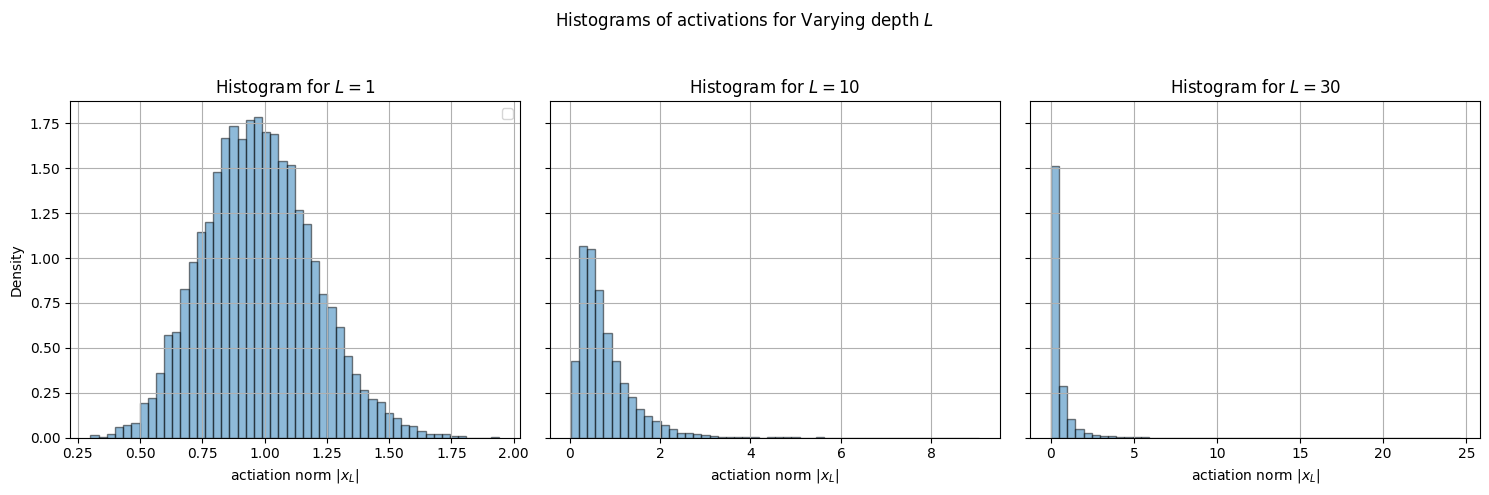
\includegraphics[width=0.8\textwidth]{./MLP_linear_forward_hist.png}
    \caption{Histogram of forward pass activations \( \|x_L\| \) for width \( d=10 \), random choices of Gaussian weights, and a uniformly drawn unit vector as input \( \|x_0\|=1 \). Depth \( L \) is varied to see the effect on the distribution.}
    \label{fig:MLP_hist}
\end{figure}

\begin{remark}
As shown in Figure \ref{fig:MLP_hist}, when the depth is small (\( L=1 \)), the mean calculated earlier predicts the actual values of our activations. However, as the network depth increases, as demonstrated by the subfigure for \( L=20 \), the distribution becomes more heavy-tailed, while the bulk of its values are very small. If we test an even deeper network, such as \( L=100 \), more than half of the values are below 0.01, while in about 1 in every 1000 networks, the value exceeds 10. The mean activation is the average of a few unlikely events where the norm is large (\( >1 \)) and the majority of events where the value is nearly zero.
\end{remark}

In plain words, as the network depth grows, most initialized networks exhibit vanishing activations, while a small number have exploding activations. Therefore, the average behavior for a randomly initialized network is the mean between these two extremes, giving the false impression that forward activations are stable. In statistical terms, the mean value is only predictive for light-tailed symmetric distributions. As the depth grows, the distribution of activations becomes heavy-tailed and highly skewed.

\section{Stabilizing the Forward Pass via Normalization}

\begin{theorem}[Normalization for Stabilizing Forward Activations]
One remedy for stabilizing forward activations is simple normalization, which can be applied on top of our MLP activations to ensure they have constant norms:
\begin{equation}
x_{\ell+1} = W_\ell \tilde{x}_\ell, \quad \tilde{x}_\ell = \frac{x_\ell}{\|x_\ell\|_{rms}}, \quad \ell = 0, \dots, L-1.
\end{equation}
Thus, it will always hold that \( E \|x_L\|^2 = d_L \). However, the additional normalization leads to different behavior between the forward and backward passes.
\end{theorem}

\begin{remark}
This difference stems from a well-known mathematical fact: the product of a chain of Gaussian matrices converges to a rank-1 matrix as the number of these matrices increases \cite{latouche1999introduction}. Consequently, the activations for any two different inputs become increasingly aligned as the depth grows.
\end{remark}

\begin{figure}[H]
    \centering
    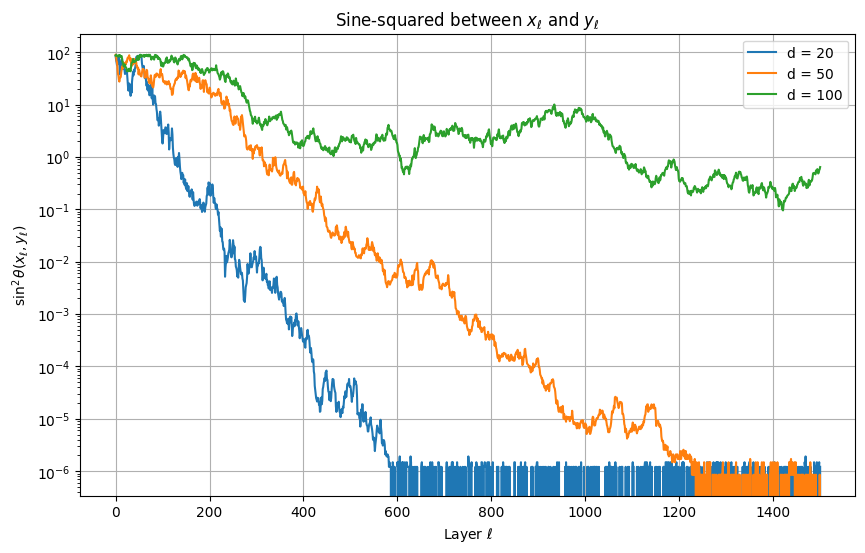
\includegraphics[width=0.8\textwidth]{./lin_MLP_collapse_sine.png}
    \caption{Mode collapse in linear MLP with normalization: for two randomly chosen inputs \( x_0 \) and \( y_0 \), we show the angle between \( x_\ell \) and \( y_\ell \) as measured by \( \sin(\theta_\ell) \). The y-axis shows sine-squared in log-scale, and the x-axis shows depth.}
    \label{fig:MLP_collapse}
\end{figure}

\begin{remark}
As shown in Figure \ref{fig:MLP_collapse}, the y-axis is in log-scale, and the linear decay in sine-squared of the angle implies an exponential convergence of \( \theta \) to 0. Thus, if we vary the weights at layer \( \ell \), the output will only change along one dimension \( W_L \dots W_{\ell+1} dW_\ell \), which is along the direction of the left singular vector of \( W_L \dots W_{\ell+1} \). This issue might seem harmless at first. However, because of the normalization at the very last layer, any changes that affect the norm of the output will be canceled out, leading to vanishing gradients, as evident in Figure \ref{fig:MLP_rank_collapse_vanishing_grads}.
\end{remark}

\begin{figure}[H]
    \centering
    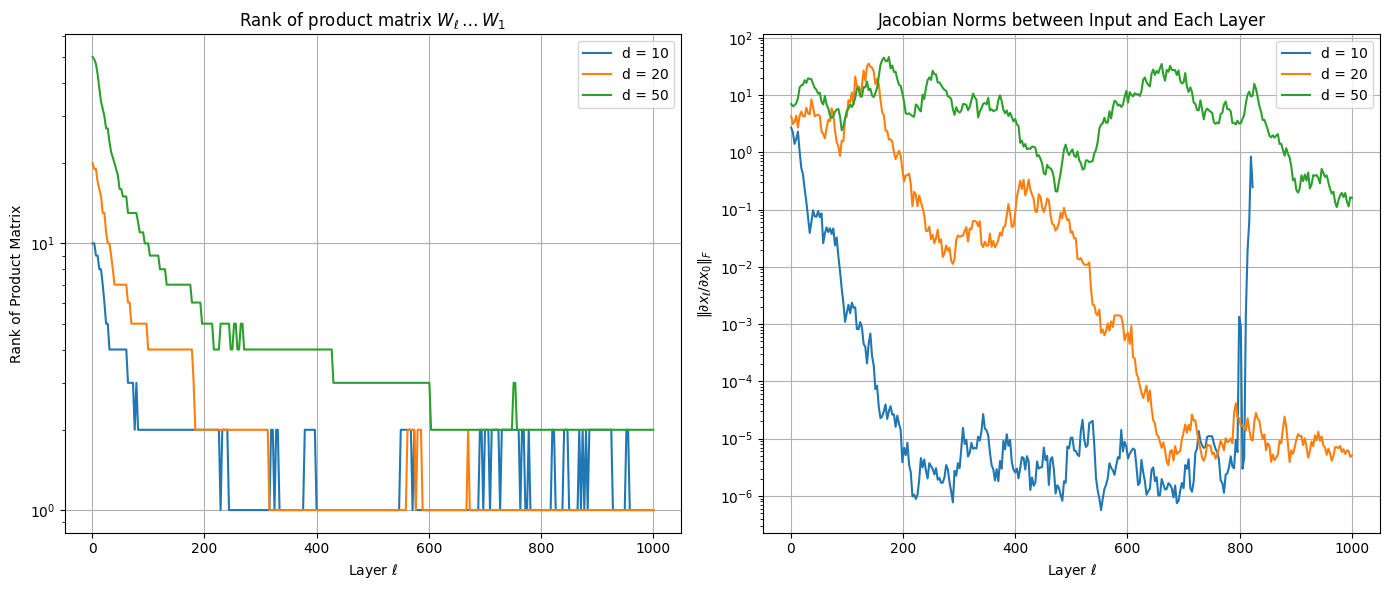
\includegraphics[width=0.8\textwidth]{./rank_collapse_vanishing_grads.png}
    \caption{In MLP with RMS normalization for forward pass, collapse of rank of Jacobian matrix, leads to vanishing gradients.}
    \label{fig:MLP_rank_collapse_vanishing_grads}
\end{figure}

\begin{theorem}[Vanishing Gradients Due to Rank-1 Convergence]
In a linear MLP with normalization layer, if the Jacobian rank collapses to 1, the gradients vanish.
\end{theorem}

\begin{proof}
First, we can ignore all normalization layers except the last one, as adding or removing those normalization constants will not affect the output:
\begin{equation}
\tilde{x}_L = \frac{x_L}{\|\tilde{x}_L\|_{rms}}, \quad x_{\ell+1} = W_\ell x_\ell \quad \ell = 0, \dots, L-1.
\end{equation}
The only difference will be in the introduction of the last normalization layer, which we can focus on analyzing:
\begin{equation}
\tilde{x} := \frac{x}{\|x\|_{rms}} \implies \frac{\partial \tilde{x}}{\partial x} = \frac{1}{\|x\|} \left( I - \frac{1}{d}(x/\|x\|)^{\otimes 2} \right).
\end{equation}
We can focus on understanding \( \partial \tilde{x}_L/\partial x_\ell \). Let \( P := W_L \dots W_0 \) and \( Q := W_L \dots W_{\ell+1} \). We thus have:
\begin{equation}
\begin{aligned}
\frac{\partial \tilde{x}_L}{\partial x_{\ell+1}} &= \frac{\partial \tilde{x}_L}{\partial x_L}\frac{\partial x_L }{\partial x_{\ell+1}} \\
&= \|x_L\|^{-1}_{rms} Q -\frac{1}{d_L}\|x_L\|^{-3}_{rms} x_L x_L^\top Q \\
&= Q / \| P x_0\|_{rms} -  \frac{1}{d} P x_0 x_0^\top P^\top Q / \| P x_0\|^{3}_{rms}.
\end{aligned}
\end{equation}
As the distance between \( \ell \) and \( L \) grows, as shown by \cite{latouche1999introduction}, the product converges to a rank-1 matrix. In the extreme case where \( Q \) is exactly a rank-1 matrix, we can prove that the gradients completely vanish. Assume \( Q = W_L \dots W_{\ell+1} = u v^\top \), where \( u \) and \( v \) are vectors. Since \( P = Q (W_\ell \dots W_0) \), \( P \) is also a rank-1 matrix: \( P = u w^\top \), where \( w = (W_\ell \dots W_0)^\top v \). Let us assume without loss of generality that \( \|u\| = 1 \). Thus, we have:
\begin{equation}
\begin{aligned}
\frac{\partial \tilde{x}_L}{\partial x_{\ell+1}}  
&= u w^\top / \| u v^\top x_0\|_{rms} -  \frac{1}{d} u v^\top x_0 x_0^\top v u^\top  u w^\top / \| u v^\top x_0\|^{3}_{rms} \\
&= u w^\top / (v^\top x_0 /\sqrt{d}) - u ((v^\top x_0)/\sqrt{d})^2 w^\top / ( v^\top x_0/\sqrt{d})^{3} \\
&= u w^\top / (v^\top x_0 /\sqrt{d}) - u w^\top / (v^\top x_0 /\sqrt{d}) \\
&= 0.
\end{aligned}
\end{equation}
If we expand the backward gradients, we have:
\begin{equation}
\frac{\partial \mathcal{L}(x_L)}{\partial W_\ell} = \frac{\mathcal{L}(x_L)}{\partial x_L}\frac{\partial x_L}{\partial \tilde{x}_{\ell+1}}\frac{\partial x_{\ell+1}}{\partial W_\ell} = 0.
\end{equation}
This notion of vanishing gradients can be refined to account for the "distance" to a rank-1 matrix.

Thus, the convergence of the matrix products \( W_L \dots W_{\ell+1} \) to a rank-1 matrix leads to a vanishing gradients problem. This case highlights the importance of analyzing and understanding backward gradients, even when the forward pass is stable. This example illustrates that if we try to normalize the forward pass when the gradients converge to a rank-1 structure, it will lead to a vanishing gradient problem.
\end{proof}


\section{Modeling Long-Tailed Distributions as Geometric Brownian Motion}

\begin{remark}
Many of the emerging phenomena related to matrix products can be viewed through the lens of geometric Brownian motion. In its basic form, geometric Brownian motion models a variable at time \( t \) as \( X_{t} = r_t X_{t-1} \), where \( r_t \) is a log-normal random variable \( \log(r_t) \sim N(\mu, \sigma^2) \), and is used as a simple model to capture price movements at small time scales. Assuming \( X_1=1 \) and taking the logarithm, we have \( \log(X_t) = \log(r_t) + \dots + \log(r_1) \), which is a sum of iid Gaussian variables, and follows \( \log(X_t) \sim N(\mu t, t\sigma^2) \).
\end{remark}

\begin{theorem}[Expected Value of Geometric Brownian Motion]
Using the moment-generating function of the normal distribution, we find that:
\begin{equation}
E[X_t] = E[e^{\log(X_t)}] = \exp(\mu t + \sigma^2 t^2 / 2).
\end{equation}
Thus, even when \( \mu < 0 \), for sufficiently large values of \( \sigma^2 \), the expectation of \( X_t \) can be very large, while \( \log(X_t) \) on average will be a negative value \( \mu t \). This results from the exponential function making the distribution of normal values highly skewed, so its mean value is an average of unlikely large values and likely small values.
\end{theorem}

\begin{remark}
This behavior is analogous to the case of the linear MLP, where the expected forward pass is constant, but in almost all cases, the forward pass is very small. This analogy is not coincidental; there are concrete principles connecting these two examples.
\end{remark}

\subsection{Corollary: Vanishing Norm of Activations}

\begin{corollary}
Let \( W_0, \dots, W_L \) be a set of \( d \times d \) Gaussian matrices with elements drawn from \( N(0, 1/d) \). Suppose \( x_0 \in \mathbb{R}^{d_0} \) is an arbitrary unit vector, \( \|x_0\| = 1 \). Then the norm of activations \( x_\ell = W_\ell \dots W_0 x_0 \) will, in most cases, have a very small value as \( \ell \) grows. Specifically, we have:
\begin{equation}
\lim_{\ell\to\infty} E \left[\log \|x_L\|_{rms}^2\right] = -\sum_{\ell=1}^L \frac{1}{2d_\ell} + o(1),
\end{equation}
where the \( o(1) \) term goes to zero with a rate of \( \sum_{\ell=1}^L 1/d_\ell^2 \).
\end{corollary}

\begin{proof}
We can model the evolution of the length of \( \|x_\ell\| \) as it passes through layers. Let \( W \) be one of the Gaussian layers with an SVD decomposition \( W = \sum_{i=1}^d s_i u_i v_i^\top \), where \( x \) is a non-zero input vector, and \( x' = W x \). We want to understand the distribution of norm-ratios \( \|x'\|^2/\|x\|^2 \). Assuming \( x \) is perfectly parallel to one of the right singular vectors of the weight matrix \( W \), i.e., one of the \( u_i \)'s chosen at random, we approximate the log-ratios by averaging the log-singular values of the weight matrix:
\begin{equation}
\log (\|x'\|^2/\|x\|^2) \approx \frac{1}{d} \sum_{i=1}^d \log(s_i^2(W)).
\end{equation}
Thus, the effect on the \( L \)-th layer will be approximately:
\begin{equation}
\log(\|x_L\|^2/\|x_0\|^2) \approx \sum_{\ell=1}^L \frac{1}{d} \log \det(W_\ell^\top W_\ell).
\end{equation}
Since the expected log-determinant of \( W_\ell^\top W_\ell \), a Wishart matrix, can be calculated in closed form, we have:
\begin{equation}
E\left[\log \det(W^\top W)\right] = n \log(2/d) + \sum_{i=0}^{n-1} \psi\left(\frac{d-i}{2}\right), \quad W \in \mathbb{R}^{d \times n}, W_{ij} \sim N(0, 1/d).
\end{equation}
From this, we conclude:
\begin{equation}
\log(\|x_L\|/\|x_0\|) \approx -\Theta(L),
\end{equation}
leading to the stated corollary.
\end{proof}

\subsection{Corollary: Convergence of Angles between Activations}

\begin{corollary}
Let \( x_0 \) and \( y_0 \) be two randomly chosen input vectors that are orthogonal, and let \( x_\ell \) and \( y_\ell \) denote their corresponding activations at layer \( \ell \). The angle between these representations, measured by \( \sin(\theta_\ell) \), converges as follows:
\begin{equation}
\lim_{\ell\to\infty} E \left[\log \sin(\theta_\ell)^2\right] =  -\sum_{\ell=1}^L \frac{1}{2d_\ell} + O\left(\frac{1}{\sum_{\ell=1}^L d_\ell^2}\right).
\end{equation}
\end{corollary}

\begin{proof}
Form the matrix \( X_\ell \) with \( x_\ell \) and \( y_\ell \) as its first and second columns. Note that \( \det(X_\ell^\top X_\ell) \) can be decomposed into \( \|x_\ell\|^2\|y_\ell\|^2 \cdot (1-\cos(\theta_\ell)^2) \). Thus we can write:
\begin{equation}
\log(1-\cos^2(\theta_\ell)) = \log \det(X_\ell^\top X_\ell) - \log\|x_\ell\|^2 - \log\|y_\ell\|^2.
\end{equation}
Taking expectations and simplifying, we obtain:
\begin{equation}
E \left[\log \sin^2(\theta_\ell)\right] =  -\sum_{\ell=1}^L \frac{1}{2d_\ell} + O\left(\frac{1}{\sum_{\ell=1}^L d_\ell^2}\right).
\end{equation}
\end{proof}

\section{Non-Asymptotic Bounds for Eigenvalues}

\begin{remark}
While the analysis of matrix products has often been conducted in asymptotic regimes, there is a growing demand for non-asymptotic analysis of neural networks due to their relatively small size compared to asymptotic assumptions. Here, we show that the same framework for analyzing log-determinants, or log-average singular values, can be surprisingly easy to convert to non-asymptotic bounds by relying on simple facts such as their sub-exponential behavior.
\end{remark}

\subsection{Corollary: Log-Determinant for Gaussian Matrices}

\begin{corollary}
Let \( W \in \mathbb{R}^{d \times n} \) be a matrix whose rows are drawn iid from \( N(0, \Sigma) \). When \( n/d \) is sufficiently small, the log-determinant of \( W^\top W \) is normally distributed with mean and variance given by:
\begin{equation}
\log \det(W^\top W/d) \to N\left(\log \det \Sigma - \frac{n^2}{2d}, \frac{2n}{d}\right).
\end{equation}
\end{corollary}

\subsection{Corollary 1: Norm Ratio of Linear MLP}

\begin{corollary}
In the setting of a linear MLP, the quantity \( \log(\|x_L\|^2/\|x_0\|^2) \) will be within a \( \sqrt{\sum_{\ell=1}^L\frac{2}{d_\ell}} \)-vicinity of \( -\sum_{\ell=1}^L\frac{1}{2d_\ell} \) with high probability:
\begin{equation}
\log(\|x_L\|^2/\|x_0\|^2) \to N\left(-\sum_{\ell=1}^L \frac{1}{2d_\ell}, \sum_{\ell=1}^L \frac{2}{d_\ell}\right).
\end{equation}
\end{corollary}

\begin{proof}
Let \( x \in \mathbb{R}^{d_1} \) and \( W \) be a \( d_2 \times d_1 \) Gaussian matrix with elements drawn from \( N(0,1/d_1) \). Define \( y = W x \), a \( d_2 \)-dimensional vector whose elements are drawn from \( N(0,\|x\|^2) \). The log-det central limit theorem (CLT) implies:
\begin{equation}
\log(\|y\|^2/d_2) \to N(\log\|x\|^2 - \frac{1}{2d_2}, \frac{2}{d_2}).
\end{equation}
Summing these normal variables across layers \( W_L \dots W_1 x_0 \) yields:
\begin{equation}
\log(\|x_L\|^2/\|x_0\|^2) \to N\left(-\sum_{\ell=1}^L \frac{1}{2d_\ell}, \sum_{\ell=1}^L \frac{2}{d_\ell}\right).
\end{equation}
Thus, \( \log(\|x_L\|^2/\|x_0\|^2) \) will be within a \( \sqrt{\sum_{\ell=1}^L\frac{2}{d_\ell}} \)-vicinity of \( -\sum_{\ell=1}^L \frac{1}{2d_\ell} \) with high probability.
\end{proof}

\subsection{Corollary 2: Angle Between Activations in MLP}

\begin{corollary}
Let \( X_0 \in \mathbb{R}^{d \times 2} \) represent two inputs \( x \) and \( y \), and let \( X_\ell \) denote the activations of these two inputs at various layers of the linear MLP. The angle between two representations in layers obeys the following universality:
\begin{equation}
\log(\sin^2\theta_L/\sin^2\theta_0) \to N\left(-\sum_{\ell=1}^L\frac{1}{d_\ell}, \sum_{\ell=1}^L \frac{8}{d_\ell}\right).
\end{equation}
\end{corollary}

\begin{proof}
Let \( X \) and \( Y = X W \) denote two successive activations where \( W \) is a \( d_1 \times d_2 \) matrix with elements drawn from \( N(0, 1/d_1) \). Each row of \( Y \) is drawn iid from \( N(0, X^\top X) \), and the log-det CLT implies:
\begin{equation}
\log \det(Y^\top Y) \to N(\log \det(X^\top X) - \frac{2}{d_2}, \frac{4}{d_2}).
\end{equation}
Successive application gives:
\begin{equation}
\log \det(X_L^\top X_L) - \log \det(X_0^\top X_0) \to N\left(-\sum_{\ell=1}^L \frac{2}{d_\ell}, \sum_{\ell=1}^L \frac{4}{d_\ell}\right).
\end{equation}
For columns \( x_\ell \) and \( y_\ell \), we obtain:
\begin{equation}
\log \|x_L\|^2 + \log \|y_L\|^2 - (\log \|x_0\|^2 + \log \|y_0\|^2) \to N\left(-\sum_{\ell=1}^L \frac{1}{d_\ell}, \sum_{\ell=1}^L \frac{4}{d_\ell}\right).
\end{equation}
Since \( \det(X_\ell^\top X_\ell) \) can be expressed as \( \det([1 \cos\theta_\ell; \cos\theta_\ell, 1]) \|x_\ell\|^2 \|y_\ell\| \), we have:
\begin{equation}
\log(\sin^2\theta_L/\sin^2\theta_0) \to N\left(-\sum_{\ell=1}^L\frac{1}{d_\ell}, \sum_{\ell=1}^L \frac{8}{d_\ell}\right).
\end{equation}
\end{proof}

\section{Batch Normalization}

\subsection{Big BN Hypothesis}

\begin{theorem}[Big BN Hypothesis]
The behavior of batch normalization (BN) in deep neural networks can be summarized in the following observations:
\begin{enumerate}
    \item If the rank of the input matrix \( X \) is small (say \( r < n \)), the process of fully connected layers plus batch normalization behaves similarly to the case where the batch size is explicitly equal to \( r \). This is because projecting points lying on an \( r \)-dimensional plane in \( \mathbb{R}^n \) onto a sphere is effectively the same as projecting points in the reduced \( r \)-dimensional space onto a sphere, modulo the radius of the sphere. The BN operation cancels out any constant scaling per layer, so this additional scale does not change the per-layer dynamics.
    \item Every small-ish eigenvalue of the Gram matrix \( \lambda_i(X^\top X) \) that is smaller than 1 undergoes an expected improvement in the mean-field regime such that its logarithm improves by \( c/n \) for some constant \( c \). However, due to the limited size \( d \), the log-eigenvalues of the weight matrix covariance are, on average, \( -n/2d \). The convolution of the two implies that small-ish eigenvalues change by \( c/n - n/2d \). If \( d = \Omega(n^2) \), the dynamics of the smallest eigenvalue will be positive until it is no longer small, giving a rate of \( r = c/n - n/2d > 0 \) per layer, and it would take \( O(-\log(\lambda_i(\text{input}))/r) \) layers to bring this eigenvalue to a constant value.
    \item Combining the first two observations, when \( d \) is not sufficiently large and \( r < 0 \), smaller eigenvalues vanish at a rate of \( -\log(\lambda(\text{layer}\ell))\approx r \ell \). Once a sufficient number of eigenvalues vanish, the rank stabilizes at approximately \( \sqrt{d} \), and adding more layers will not significantly change the rank.
\end{enumerate}
\end{theorem}

\subsection{Speculative Refinement}

\begin{remark}
The improvement in the infinite width regime is \( c/n (1-\lambda) \), implying larger eigenvalues have smaller expected improvement, and smaller ones have larger improvement. This induces a stochastic dynamic where smaller eigenvalues grow and larger ones shrink, suggesting that the dynamic is more accurate for the determinant or mean log-eigenvalue.

If we use orthogonal fully connected layers instead of Gaussian layers, the \( -n/2d \) component is absent, which would roughly add \( c/n \) to the log-minimum eigenvalue per layer, or more accurately \( c/n (1-\lambda) \).

When the eigenvalues are sufficiently close to 1, the mean-field dynamics shrink the log-eigenvalues by a constant \( (1-c/n) \) factor, reducing the variance by the same amount. Non-mean-field dynamics add variance of \( n/d \) to the distribution. Thus, the variance of eigenvalues is approximately \( n^2/d \), and their mean is approximately \( -n/d \) at equilibrium.
\end{remark}

\section{Batch Normalization Analysis}

\begin{remark}
Let \( X \) represent a batch normalization operation, where \( X \) is a \( d \times n \) Gaussian matrix with rows drawn iid from \( N(0,\Sigma) \), and \( D \) is a diagonal matrix with \( D_{ii}=1/\|row_i(X)\|_{rms} \). The SVD decomposition of \( DX = D U S V^\top \) leads to:
\begin{equation}
(DX)^\top (DX)  = V^\top S U^\top D^2 U S V.
\end{equation}
Thus, the spectral values are equal to \( U^\top D^2 U (S V^\top S) \), and we have:
\begin{equation}
\log \left[\det\left((DX)^\top (DX)\right)\right] = \log \det(X^\top X) + \log \det\left(U^\top D^2 U\right).
\end{equation}
The first term is simply \( \log \det(X^\top X) \), and the second term is given by the following corollary.
\end{remark}

\subsection{Corollary: Sub-Rotation Log-Determinant}

\begin{corollary}
Suppose \( D \) is a \( d \times d \) matrix, and \( U \) is a random rotation matrix of size \( d \times n \). If \( d \) is divisible by \( n \), then the expected log-determinant of the projection of \( A \) onto the columns of \( U \) is \( n/d \) times the log-volume of \( D \):
\begin{equation}
E \left[\log\left(U^\top D^2 U\right)\right] = \frac{n}{d} \log \det(D^2).
\end{equation}
\end{corollary}

\begin{proof}
If \( d \) is divisible by \( n \), let \( M \in \mathbb{R}^{d \times d} \) be a random rotation matrix. Since \( U \) is a rotation, the spectrum of \( M^\top D \) is equal to the spectrum of \( D \), so \( \det(M^\top D^2 M) = \det(D^2) \).

Let \( M_1, \dots, M_{d/n} \) be the columns packed into \( n \)-sized columns. Since the index of the columns of \( M \) is meaningless, we conclude:
\begin{equation}
E \left[\log\left(M_1^\top D^2 M_1\right)\right] = \frac{n}{d} \log \det(D^2).
\end{equation}
\end{proof}

\section{MLP with Non-Linear Activation}

\begin{remark}
We now extend the analysis to a linear MLP with non-linear activation functions, focusing on the leaky ReLU:
\begin{equation}
f(x) = \begin{cases} x & x \ge 0 \\ \alpha x & x < 0 \end{cases}.
\end{equation}
The forward pass is modeled as \( \log(\|f(W x) \|^2) \), with:
\begin{equation}
\log(\|D W x \|), \quad D_{ii} = diag(f'(x_i))_{i \le n}.
\end{equation}
\end{remark}

\subsection{Lemma: Expected Log-Determinant of Wishart}

\begin{lemma}
If \( W \) is a \( d \times n \) matrix whose elements are drawn iid from \( N(0, 1/d) \), then:
\begin{equation}
E \left[\log \det(W^\top W)\right] = n \log(2) - n \log(d) + \sum_{i=1}^n \psi\left(\frac{d-i+1}{2}\right),
\end{equation}
where \( \psi \) is the digamma function. As an approximation for \( n < d \), we have:
\begin{equation}
E \left[\log \det(W^\top W)\right] = -\frac{n^2}{2d} - \frac{n^3}{6d^2} - \frac{n^4}{3 d^3} + O\left(\frac{n^5}{d^4}\right),
\end{equation}
which becomes more accurate as \( n/d \) decreases.
\end{lemma}

\begin{remark}
Note that the approximation for the normalized log-determinant \( \frac{1}{n} E \left[\log \det(W^\top W)\right] \) depends only on the ratio \( n/d \), meaning the log-determinant, in expectation, does not change if we keep the ratio fixed.
\end{remark}

\begin{proof}
In \cite{braun2010variational}, the authors calculated:
\begin{equation}
\Lambda \sim \mathcal{W}_D(v, \Psi) \implies E \left[\log \det(\Lambda)\right] = D \log(2) + \log\det(\Psi) + \sum_{i=1}^D \psi\left(\frac{\nu-i+1}{2}\right),
\end{equation}
where \( \nu \) is the degrees of freedom, and \( \nu\Psi \) is the mean \( E[\Lambda] = \nu\Psi \). For \( W \) of size \( d \times n \), with \( W_{ij} \sim N(0, 1/d) \), \( E[W^\top W] = I_n \) and it has \( m \) degrees of freedom. So \( \Psi = I_n / d \). Therefore, \( \det(\Psi) = (1/d)^n \implies \log \det(\Psi) = n \log(1/d) \), and thus we have:
\begin{equation}
E \left[\log \det(W^\top W)\right] = n \log(2) - n \log(d) + \sum_{i=1}^n \psi\left(\frac{d-i+1}{2}\right).
\end{equation}
Using the approximation:
\begin{equation}
\psi(z) \approx \log(z) - \frac{1}{2z} - \frac{1}{12 z^2} + \dots,
\end{equation}
and assuming \( d \gg n \), this leads to:
\begin{equation}
E \left[\log \det(W^\top W)\right] \approx -\frac{n^2}{2d} - \frac{n^3}{6d^2} - \frac{n^4}{3d^3} + O\left(\frac{n^5}{d^4}\right).
\end{equation}
For \( n=d \), we have:
\begin{equation}
\frac{1}{d} E \left[\log \det(W^\top W)\right] \approx -1, \quad W \in \mathbb{R}^{d \times d}.
\end{equation}
\end{proof}

\subsection{Central Limit Theorem for Log-Determinant}

\begin{theorem}[CLT for Log-Determinant]
A central limit theorem (CLT) is established for the log-determinant of \( W^\top W \), where \( W \) is a \( d \times n \) matrix with elements drawn iid from \( N(0, 1/d) \) in the high-dimensional setting where the dimension \( n \) grows with the sample size \( d \), with the only restriction that \( n(d) \leq d \). Specifically:
\begin{equation}
\frac{\log \det (W^\top W) - \sum_{i=1}^{d} \log \left(1 - \frac{i}{d}\right)}{\sqrt{-2\log(1-n/d)}} \xrightarrow{distr.} N(0,1) \text{ as } n \to \infty.
\end{equation}
For the boundary case \( n=d \):
\begin{equation}
\frac{\log \det (W^\top W) -\log(n-1)! + n \log n}{\sqrt{2\log n}} \xrightarrow{distr.} N(0,1) \text{ as } n \to \infty.
\end{equation}
\end{theorem}

\begin{remark}
When \( n/d \) is sufficiently small, we have:
\begin{equation}
\log\det(W^\top W) \to N\left(-\frac{n^2}{2d}, \frac{2n}{d}\right).
\end{equation}
For \( n=d \), the distribution is given by:
\begin{equation}
\log\det(W^\top W) \approx N\left(-\log(n-1)! + n \log n, 2\log n\right).
\end{equation}
\end{remark}

\begin{proof}
The result is derived using the central limit theorem for log-determinants of random matrices with iid standard Gaussian entries, as shown in \cite{hazra2019det}. The case when \( n/d \) is small is derived using asymptotic expansions of the digamma function.
\end{proof}

% !TEX root = ../thesis-index.tex


\chapter{Batch Normalization Orthogonalizes Representations}\label{ch:bn_ortho}

Batch Normalization (BN)~\citep{ioffe2015batch} enhances training across a wide range of deep network architectures and experimental setups~\citep{he2016deep,huang2017densely,silver2017mastering}. The practical success of BN has inspired research into the underlying mechanism of BN~\citep{santurkar2018does,karakida2019normalization,arora2018theoretical,bjorck2018understanding}.
BN influences first-order optimization methods by avoiding the rank collapse in deep representation \citep{daneshmand2020batch},  direction-length decoupling of optimization \citep{kohler2018exponential}, influencing the convergence of the steepest descent  \citep{arora2018theoretical,bjorck2018understanding}, and smoothing the optimization objective function \citep{santurkar2018does,karakida2019normalization}. However, the benefits of BN go beyond its critical role in optimization. For example, \cite{frankle2020training} shows that BN networks with random weights also achieve surprisingly high performance after only minor adjustments of their weights. This striking result motivates us to study the representational power of random networks with BN.  


We study hidden representations across layers of a laboratory random BN with linear activations. Consider a batch of samples passing through consecutive BN and linear layers with Gaussian weights. The representations of these samples are perturbed by each random linear transformation, followed by a non-linear BN. At first glance, the deep representations appear unpredictable after many stochastic and non-linear transformations. Yet, we show that these transformations orthogonalize the representations. To prove this statement, we introduce the notion of  ``orthogonality gap'', defined in Section \ref{ortho:sec:orthogonality}, to quantify the deviation of representations from a perfectly orthogonal representation. Then, we prove that the orthogonality gap decays exponentially with the network depth and stabilizes around a term inversely related to the network width. More precisely, we prove 
\begin{align} \nonumber
     \E\Bigg[ \text{orthogonality gap} \Bigg] = \bigo\left( \left(1-\alpha\right)^{\text{depth}}+ \frac{\text{batchsize}}{\alpha\sqrt{\text{width}}}\right)
\end{align}
holds for $\alpha>0$ that is an absolute constant under a mild assumption. In probability theoretic terms, we prove stochastic stability of the Markov chain of hidden representations \citep{kushner1967stochastic,kushner2003stochastic,khasminskii2011stochastic}. The orthogonality of deep representations allows us to prove that the distribution of the representations after linear layers contracts to a Wasserstein-2 ball around isotropic Gaussian distribution as the network depth grows. Moreover, the radius of the ball is inversely proportional to the network width. Omitting details, we prove the following bound holds:
\begin{align} \nonumber
    \text{Wasserstein}_2(\text{representations},\text{Gaussian})^2= \bigo\left( \left(1-\alpha\right)^{\text{depth}}\left(\text{batchsize}\right)+ \frac{ (\text{batchsize})^2}{\alpha\sqrt{\text{width}}}\right).
\end{align}
The above equation shows how depth,  width, and batch size, interact with the Gaussian approximation of the representations. Since the established rate is exponential with depth, the distribution of the representations stays in a Wasserstein ball around isotropic Gaussian distribution after a few layers. Thus, BN not only stabilizes the distribution of the representations, which is its main promise~\citep{ioffe2015batch}, but also enforces Gaussian isotropic distribution in deep layers. 

There is growing interest in bridging the gap between neural networks, as the most successful parametric methods for learning, and Gaussian processes and kernel methods, as well-understood classical models for learning \citep{jacot2018neural,matthews2018gaussian,lee2017deep,bietti2019inductive,huang2014kernel}. This link is inspired by studying random neural networks in the asymptotic regime of infinite width. The seminal work by \cite{neal2012bayesian} sparks that a single-layer network resembles a Gaussian process as its width goes to infinity. However, increasing the depth may significantly shift the distribution of the representations away from Gaussian \citep{ioffe2015batch}. This distributional shift breaks the link between Gaussian processes and deep neural networks. To ensure Gaussian representations,  \cite{matthews2018gaussian} suggests increasing the width of the network proportional to the network depth. Here, we show that BN ensures Gaussian representations even for deep networks with \textit{finite} width. This result bridges the link between deep neural networks and Gaussian processes in the regime of finite width. Many studies rely on deep Gaussian representations in an infinite width setting \citep{yang2018a,schoenholz2016deep,pennington2018emergence,klambauer2017self,de2018random}. Our non-asymptotic Gaussian approximation can be incorporated into their analysis to extend these results to the regime of finite width.

Since training starts from random networks,  representations in these networks directly influence training. Hence, recent  theoretical studies has investigated the interplay between initial hidden representations and training~\citep{daneshmand2020batch,bjorck2018understanding,frankle2020training,schoenholz2016deep,saxe2013exact,bahri2020statistical}.
In particular, it is known that hidden representations in random networks \emph{without BN} become correlated as the network grows in depth, thereby drastically slowing training~\citep{daneshmand2020batch,he2016deep,bjorck2018understanding,saxe2013exact}. 
On the contrary,  we prove that deep representations in networks \emph{with BN} are almost orthogonal.
We experimentally validate that initial orthogonal representations can save training time that would otherwise be needed to orthogonalize them. By proposing a novel initialization scheme, we ensure the orthogonality of hidden representations. Such an initialization effectively avoids the training slowdown with depth for vanilla networks, with no need for BN.  This observation further motivates studying the inner workings of BN to replace or improve it for deep learning. \\
Theoretically, we made the following contributions:
\begin{enumerate}
    \item  For MLPs with batch normalization, linear activation, and Gaussian weights, we prove that representations across layers become increasingly orthogonal up to a constant inversely proportional to the network width. 
    \item Leveraging the orthogonality, we prove that the distribution of the representations contracts to a Wasserstein ball around a Gaussian distribution as the depth grows. Up to the best of our knowledge,  this is the first \textit{non-asymptotic} Gaussian approximation for deep neural networks with finite width.
\end{enumerate}
Experimentally, we made the following contribution\footnote{Implementations are available at \href{https://github.com/hadidaneshmand/batchnorm21.git}{https://github.com/hadidaneshmand/batchnorm21.git}}: 
\begin{enumerate}[resume]
    \item  Inspired by our theoretical understanding, we propose a novel weight initialization for standard neural networks that ensure orthogonal representations without BN. Experimentally, we show that this initialization effectively avoids training slowdown with depth in the absence of BN. 
\end{enumerate}






% Studying input representation in deep random neural network has been subject of many theoretical and practical studies \cite{matthews2018gaussian,lee2017deep,klambauer2017self,hazan2015steps,daniely2016toward,saxe2013exact,schoenholz2016deep,bahri2020statistical,daneshmand2020batch}. Without BN, representations become aligned in deep layers of random networks that pose optimization challenges~\cite{daneshmand2020batch,bjorck2018understanding,frankle2020training}. Yet, 


% \textit{Random} neural networks have been the focus of many theoretical and practical studies \cite{neal2012bayesian,matthews2018gaussian,lee2017deep,klambauer2017self,hazan2015steps,daniely2016toward,saxe2013exact,schoenholz2016deep,bahri2020statistical}. Random networks exhibit interesting theoretical properties such as having exponential expressive power with depth \cite{express17}, they are approximately Gaussian processes \cite{neal2012bayesian}, and closed tied to random matrix theory \cite{louart2018random}. In particular, as the initialization of training deep networks, properties of random networks play a direct role in the training algorithm. As the depth increase representation become aligned in deep neural networks which pose challenges.  Batch Normalization (BN) \cite{ioffe2015batch} improves training deep neural networks for a wide class of networks and learning problems. Recent studies link the enhanced training performance with BN to disentangled representations in random deep BN networks \cite{daneshmand2020batch,bjorck2018understanding,frankle2020training}, while entangled representations in deep networks drastically slow down the training process \cite{daneshmand2020batch,schoenholz2016deep,saxe2013exact,bahri2020statistical}. Inspired by these remarkable findings,  we study representations in random deep networks with BN.
% \input{sections/1_Introduction}



\section{Preliminaries} \label{ortho:sec:perliminaries}
\subsection{Notations}
Akin to~\cite{daneshmand2020batch}, we focus on a Multi-Layer Perceptron (MLP) with batch normalization and linear activation. Theoretical studies of linear networks is a growing research area~\citep{saxe2013exact,daneshmand2020batch,bartlett2019gradient,arora2018convergence}.  When weights are initialized randomly, linear and non-linear networks share similar properties such as the rank collapse issue studied in~\citep{daneshmand2020batch}. For ease of analysis, we assume activations are linear. 
% argue that our findings extend to non-linear in Section~\ref{ortho:sec:activations}.

We use $n$ to denote batch size, and $d$ to denote the width across all layers, which we further assume is larger than the batch size $d\geq n$. Let $H_\ell \in \R^{d\times n}$ denote representations for $n$ samples in layer $\ell$, with $H_0 \in \R^{d \times n}$ corresponding to $n$ input samples in the batch with $d$ features. Successive representations are connected by Gaussian weight matrices $W_\ell\sim\Normal(0,I_d/d)$ as 
\begin{align}
    \label{ortho:eq:chain_linear}
    H_{\ell+1} = \frac{1}{\sqrt{d}} BN(W_{\ell} H_{\ell}), \quad BN(M) = \diag(M M^\top)^{-\sfrac{1}{2}} M,
\end{align}
where $\diag(.)$ zeros out off-diagonal elements of its input matrix, and the scaling factor $1/\sqrt{d}$ ensures that all matrices $\{H_k\}_{k}$ have unit Frobenius norm (see Section~\ref{ortho:sec:perliminaries}). The BN function in Eq.~(\ref{ortho:eq:chain_linear}) differs slightly from the commonly used definition for BN as the mean correction is omitted. However, \cite{daneshmand2020batch} shows this difference does not change the network properties qualitatively. 
% Section~\ref{ortho:sec:activations} further discusses about the role of the mean correction term in our analysis. Readers can find all the notations in Appendix Table~\ref{ortho:tab:notations}.

\subsection{The linear independence of hidden representations}
\cite{daneshmand2020batch} observe that if inputs are linearly independent, then their hidden representations remain linearly independent in all layers as long as $d = \Omega(n^2)$. Under technical assumptions, \cite{daneshmand2020batch} establishes a lower-bound on the average of the rank of hidden representations over infinite layers. Based on this study, we assume that the linear independence holds and build our analysis upon that. This avoids restating the technical assumptions of \cite{daneshmand2020batch} and also further technical refinements of their theorems. The next assumption presents the formal statement of the linear independence property.
 \begin{assumptioncost}{1}{\alpha,\ell}
%  [check \cite{daneshmand2020batch} for the justification] 
 \label{ortho:assume:lineary_indepdence}
 There exists an absolute positive constant $\alpha$ such that the minimum singular value of $H_k$ is greater than (or equal to) $\alpha$  for all $k=1,\dots, \ell$.
\end{assumptioncost}
 
The linear independence of the representations is a shared property across all layers. However, the representations constantly change when passing through random layers. In this chapter, we mathematically characterize the dynamics of the representations across layers. 


\section{Orthogonality of deep representations} \label{ortho:sec:orthogonality}
\subsection{A warm-up observation}
To illustrate the difference between BN and vanilla networks, we compare hidden representations of two input samples across the layers of these networks. Figure~\ref{ortho:fig:orthogonality} plots the absolute value of cosine similarity of these samples across layers. This plot shows a stark contrast between vanilla and BN networks: While representations become increasingly orthogonal across layers of a BN network, they become increasingly aligned in a vanilla network. More specifically, we observe that BN is able to orthognalized almost aligned representations; while, the vanilla network provides almost align representation of two orthogonal samples in deep layers. While this behaviour has been theoretically studied for vanilla networks \citep{daneshmand2020batch,bjorck2018understanding,saxe2013exact}, up to the best of our knowledge, it is not theoretically analyzed for BN networks for networks with finite width regime. In the following section, we formalize and prove this orthogonalizing property for BN networks with finite widths.  
\begin{figure}[!ht]
    \centering
    \begin{tabular}{c}
        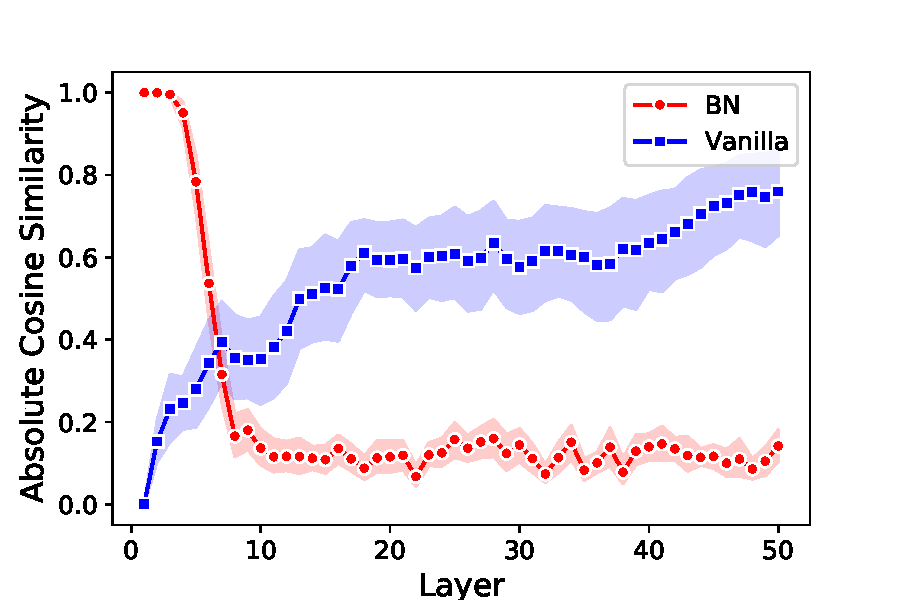
\includegraphics[width=0.4\textwidth]{figures/warmup.pdf}
    \end{tabular}
    \caption{\textbf{Orthogonality: BN vs. vanilla networks.} The horizontal axis shows the number of layers, and the vertical axis shows the absolute value of cosine similarity between two samples across the layers ($d=32$). Mean and 95\% confidence intervals of 20 independent runs.
    }
    \label{ortho:fig:orthogonality}
\end{figure}

\subsection{Theoretical analysis}
The notion of orthogonality gap plays a central role in our analysis. Given the hidden representation $H \in \R^{d\times n}$, matrix $H^\top H$ constitutes inner products between representations of different samples. Note that $H^\top H \in \R^{n \times n}$ is different form the covariance matrix $H H^\top/n \in \R^{d\times d}$. The orthogonality gap of $H$ is defined as the deviations of $H^\top H$ from identity matrix, after proper scaling. More precisely, define $V: \R^{d\times n}\setminus\mathbf{0} \to \R_+$ as 
\begin{align}
    V(H) := \Big\| \left(\frac{1}{\|H\|_F^2}\right)H^\top H - \left(\frac{1}{\|I_n\|_F^2}\right)I_n \Big\|_F.
\end{align}
% We can reformulate orthogonality gap in terms of eigenvalues of the sample covariance matrix $V(H):= \|\lambda_i/|\lambda|_1-\ones/n\|_2$, 
% where $\lambda=(\lambda_i)_{i\le n}$ are eigenvalues of $H^\top H$, and $\ones=(1)_{i\le n}$. In other words, the orthogonality gap quantifies deviations of the sample-covariance eigenvalues from their mean. For hidden representations $H_\ell$, this formula simplifies to $V(H_\ell)=\|\lambda - \ones/n\|$. Observe that $V(H)$ reaches its extreme values for perfectly orthogonal and perfectly correlated matrices $H$.  
The following theorem establishes a bound on the orthogonality of representation in layer $\ell$.
\begin{theorem} \label{ortho:thm:contraction}
Under Assumption \ref{ortho:assume:lineary_indepdence}$(\alpha,\ell)$, the following holds:
    \begin{align}\label{ortho:eq:exponential_contraction}
        \E \left[ V(H_{\ell+1}) \right] \leq 2 \left(1-\frac{2}{3}\alpha\right)^{\ell}+ \frac{3 n}{\alpha\sqrt{d}}.
    \end{align}
\end{theorem}
\noindent Assumption \ref{ortho:assume:lineary_indepdence} is studied by   \cite{daneshmand2020batch} who note that \ref{ortho:assume:lineary_indepdence}$(\alpha,\infty)$ holds as long as $d=\Omega(n^2)$. If \ref{ortho:assume:lineary_indepdence} does not hold, one can still prove that there is a function of representations that decays with depth up to a constant (see Section~\ref{ortho:sec:proof_thm}).


The above result implies that BN is an approximation algorithm for orthogonalizing the hidden representations. If we replace $\diag(M)^{-1}$  by $(M)^{-1}$ in BN formula, in Eq.~\eqref{ortho:eq:chain_linear}, then all the hidden representation will become exactly orthogonal.  However, computing the inverse of a \textit{non-diagonal} $d\times d$ matrix is computationally expensive, which must repeat for all layers throughout training, and differentiation must propagate back through this inversion. The diagonal approximation in BN significantly reduces the computational complexity of the matrix inversion. Since the orthogonality gap decays at an exponential rate with depth, the approximate orthogonality is met after only a few layers. Interestingly, this yields a desirable cost-accuracy trade-off: For a larger width, the orthogonality is more accurate, due to term $1/\sqrt{d}$ in the orthogonality gap, and also the computational gain is more significant.   



From a different angle, Theorem~\ref{ortho:thm:contraction} proves the stochastic stability of the Markov chain of hidden representations. In expectation, stochastic processes may obey an inherent Lyapunov-type of stability  \citep{kushner1967stochastic,kushner2003stochastic,khasminskii2011stochastic}. One can analyze the mixing and hitting times of Markov chains based on the stochastic stability of Markov chains,\citep{kemeny1976markov,eberle2009markov}.  
In our analysis, the orthogonality gap is a Lyapunov function characterizing the stability of the chain of hidden representations. This stability opens the door to more theoretical analysis of this chain, such as studying mixing and hitting times. For, example the stability can be used for mixing analysis of the chain $\{H_1, \dots, H_\ell,\dots \}$. Let $\pi$ denote the stationary distribution of this chain. Under a particular stochastic stability condition called geometric drift condition, 
 \begin{align*}
      \left| \E \left[ \varphi(H_\ell) \right] - \E_{H \sim \pi} \left[ \varphi(H) \right] \right| \leq \alpha^{\ell} \left| \E \left[ \varphi(H_0) \right] - \E_{H \sim \pi} \left[ \varphi(H) \right] \right|
 \end{align*}
 holds for $\alpha \in (0,1)$ and measurable function $\varphi: R^{d\times n} \to R$  (see Theorem 3.6  of \citep{hairer2010convergence}). The drift condition holds if there exists a Lyapunov function $L: R^{d\times n} \to [0,1]$ and constant $K\geq 0$ such that the following holds: 
 \begin{align*}
     E \left[ L(H_{\ell+1})| H_\ell \right] \leq \gamma L(H_{\ell}) + K. 
 \end{align*}
 We prove that the above condition holds in Eq~\eqref{ortho:eq:lyp_condition}. However, such theoretical analyses may not be of interest to the machine learning community, hence we focus on the implications of these results for understanding the underpinnings of neural networks.


It is helpful to compare the orthogonality gap in BN networks to studies on vanilla networks \citep{bjorck2018understanding,daneshmand2020batch,saxe2013exact}. The function implemented by a vanilla linear network is a linear transformation as the product of random weight matrices. The spectral properties of the product of i.i.d.~random matrices are the subject of extensive studies in probability theory~\citep{bougerol2012products}. Invoking these results, one can check that the orthogonality gap of the hidden representations in vanilla networks rapidly increases since the rank of representations converges to a one matrix as the depth grows~\citep{daneshmand2020batch}. 
% We refer readers to Section~\ref{ortho:sec:vanilla_theory} for more details about vanilla networks. 

Remarkably, \cite{agarwal2021deep} proves if activation functions obey a self-normalization property, then a specific kernel of hidden representations becomes well-condition as the network depth grows. However, it is not clear how to impose the self-normalization property. Here, we establish the whitening for an explicitly defined normalization used in practice. 



\subsection{Experimental validations}
Our experiments presented in Fig.~\ref{ortho:fig:spectral_contraction_1} validate the  exponential decay rate of $V$ with depth. In this plot, we see that $\log(V_\ell)$ linearly decreases for $\ell=1, \dots, 20$, then it wiggles around a small constant.  Our experiments in Fig.~\ref{ortho:fig:spectral_contraction_2} suggest that the $\bigo(1/\sqrt{d})$ dependency on width is  almost tight. Since $V(H_\ell)$ rapidly converges to a ball, the average of $V(H_\ell)$ over layers estimates the radius of this ball. This plot shows how the average of $V(H_\ell)$, over 500 layers, changes with the network width, validating the $\bigo(1/\sqrt{d})$ dependency implied by Theorem~\ref{ortho:thm:contraction}. 
 \begin{figure}[!ht]
     \centering
     \begin{subfigure}[b]{0.4\textwidth}
         \centering
         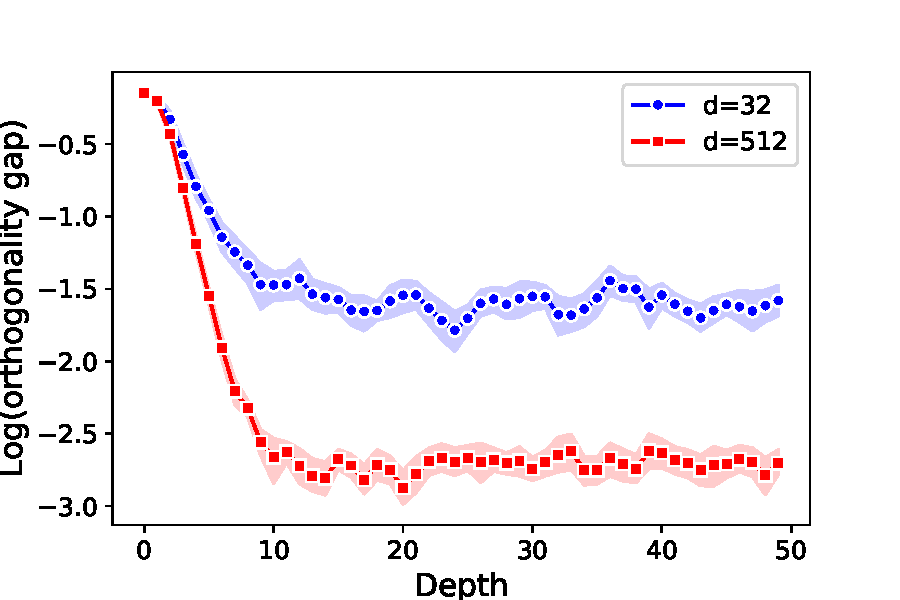
\includegraphics[width=\textwidth]{figures/gaps_depth_bn.pdf}
         \caption{Orthogonality vs. depth}
         \label{ortho:fig:spectral_contraction_1}
     \end{subfigure}
     \begin{subfigure}[b]{0.4\textwidth}
         \centering
         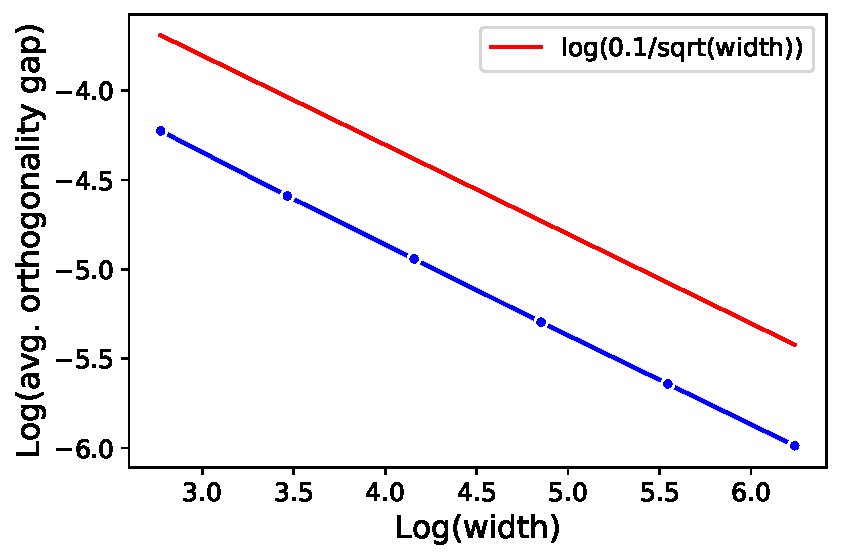
\includegraphics[width=\textwidth]{figures/gaps_width_bn.pdf}
         \caption{Orthogonality vs. width}
         \label{ortho:fig:spectral_contraction_2}
     \end{subfigure}
    \caption{\footnotesize{\textbf{Orthogonality gap vs.\ depth and width.} Left: $\log(V(H_\ell))$ vertically versus $\ell$ horizontally. Right: $\log(\frac{1}{500}\sum_{\ell=100}^{600} V(H_\ell))$ vertically versus $\log(d)$ horizontally. The chain starts from a diagonal $H_0$ with one relatively large diagonal value. This structure imposes a large orthogonality gap for $H_0$.  Mean and 95\% confidence interval of 20 independent runs.}  }
        % \label{ortho:fig:spectral_contraction}
\end{figure}

Consider an input matrix $H_0 \in \R^{d\times n}$ containing $n$ samples in $\R^d$. Assuming that elements of this matrix are i.i.d. zero-mean and unit variance random variables, the minimum singular value of $H_0$ is greater than $\sqrt{d}-\sqrt{n}$. In practical applications, the batchsize used for normalization is relatively smaller than the network width, hence  \ref{ortho:assume:lineary_indepdence}$(\Theta(1),0)$ holds. For the intermediate representations,  we also observed that  \ref{ortho:assume:lineary_indepdence}($\alpha$,$\ell$) holds --for an $\alpha$ independent from $\ell$-- as long as $d \gg n$. Let $\alpha_0$ denote the minimum singular value of $H_0$. For different values of $d$ and $n$, we check whether \ref{ortho:assume:lineary_indepdence}($0.1\alpha_0$, $1000$) holds. Fig.~\ref{ortho:fig:assumption_nd} illustrates that this assumption hold for $d= \Omega(n^2)$, which is also confirmed by \cite{daneshmand2020batch}.



\begin{figure}[!ht]
     \centering
         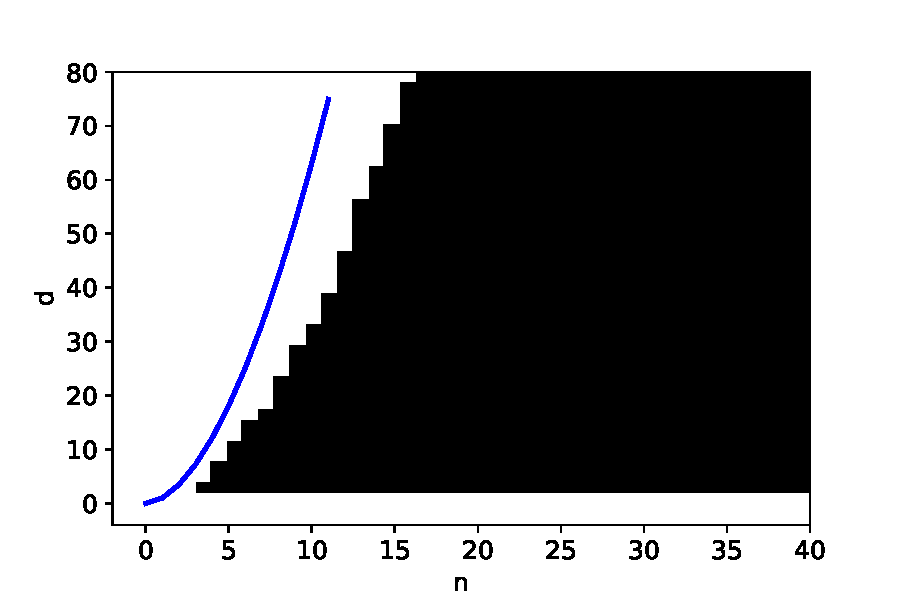
\includegraphics[width=0.5\textwidth]{figures/assumption_nd.pdf}
    \caption{\footnotesize{\textbf{Validations for \ref{ortho:assume:lineary_indepdence}} Pixel $(n,d)$ marks whether \ref{ortho:assume:lineary_indepdence} holds in all 10 independent runs: The black color indicates \ref{ortho:assume:lineary_indepdence}$(0.1\alpha_0,1000)$ failed in at least once (where $\alpha_0$ is the minimum singular value of $H_0$). The blue curve marks $d=(n-28)^{1.8}$ highlighting \ref{ortho:assume:lineary_indepdence} holds for $d = \Omega(n^2)$.} }
    \label{ortho:fig:assumption_nd}
\end{figure}



\section{Gaussian approximation} \label{ortho:sec:normal_approximation}
\subsection{Orthogonality yields Gaussian approximation}
The established result on the orthogonality gap allows us to show that the representations after linear layers are approximately Gaussian. If $H_\ell$ is orthogonal, the random matrix $W_\ell H_\ell$ is equal in distribution to a standard Gaussian matrix due to the invariance of standard Gaussian distribution under linear orthogonal transformations. We can formalize this notion of Gaussianity by bounding the Wasserstein-2 distance between the distribution of $W_\ell H_\ell$ and standard Gaussian distribution. Let $\mathcal{W}_2(R_1,R_2)$ denote the Wasserstein-2 distance between probability distributions of two random variables $R_1$, and $R_2$.
% Recall that $\mathcal{W}_2$ distance between laws of two random matrices $P, Q \in \R^{d \times n}$ is obtained by the infimum of couplings between these two random variables as
% \begin{align} \label{ortho:eq:w_distance}
%     \mathcal{W}_2\left(\law(P),\law(Q)\right)^2 = \inf_{\gamma \in \Gamma} \int \| P - Q \|_F^2 d\gamma(P, Q),
% \end{align}
% where $\Gamma$ is the set of all couplings between $\law(P)$ and $\law(Q)$ (see Chapter 1 of  \cite{villani2009optimal}). 
The next lemma formally establishes the link between the orthogonality and the distribution of the representations. 
\begin{lemma} \label{ortho:lemma:wv_bound}
Given $G \in \R^{d\times n}$ with i.i.d. zero-mean $1/d$-variance Gaussian elements, the following Gaussian approximation holds:
\begin{align}
\label{ortho:eq:bn_recurrence}
    \mathcal{W}_2\left( W_\ell H_\ell , 
    G/\sqrt{n}\right)^2 \leq 2 n \E \left[ V(H_\ell) \right].
\end{align}
\end{lemma}
Combining the above result with Theorem~\ref{ortho:thm:contraction} yields the result presented in the next corollary.
\begin{corollary} \label{ortho:cor:gaussian_approximation}
For $G \in \R^{d\times n}$ with i.i.d. zero-mean $1/d$-variance Gaussian elements, 
\begin{align}
    \mathcal{W}_2\left( W_\ell H_\ell, G/\sqrt{n}\right)^2 \leq 4n \left(1-\frac{2}{3}\alpha\right)^{\ell}+ \frac{6 n^2}{\alpha\sqrt{d}}
\end{align}
holds under Assumption~\ref{ortho:assume:lineary_indepdence}$(\alpha,\ell)$.
\end{corollary}

% \paragraph{Proof idea:} Let $H_\ell=U S V^\top$ denote the SVD decomposition of $H_\ell$ in the reduced form\footnote{We have $U\in \R^{d\times n}, S\in\R^{n\times n}, V\in\R^{n\times n}$}. If we ignore the scaling $S$ for the moment, if we transport distribution of of $W_\ell$ to $(W_\ell H_\ell)$ via rotation matrix $U$, followed by a second rotation $V^\top$ to $W_\ell (U V^\top)$, implying that $W_\ell U V^\top$ has zero Wasserstein-2 distance to $W_\ell$. The main idea is to couple weight matrix $W_\ell$ and $G$ according rotation matrices to upper bound the Wasserstein-2 distance. 


In other words, the distribution of the representations contracts to a Wasserstein 2 ball around an isotropic Gaussian distribution as the depth grows. The radius of the Wasserstein 2 ball is at most $\bigo(1/\sqrt{\text{width}})$.
As noted in the last section, \ref{ortho:assume:lineary_indepdence} is extensively studied by \cite{daneshmand2020batch} where it is shown that \ref{ortho:assume:lineary_indepdence}$(\alpha>0,\infty)$ holds as long as $d = \Omega(n^2)$. 

% Next, we compare this result with Gaussian approximations the literature. 
\subsection{Deep neural networks as Gaussian processes}
Leveraging BN, Corollary~\ref{ortho:cor:gaussian_approximation} establishes the first \textit{non-asymptotic} Gaussian approximation for deep random neural networks. For vanilla networks, the Gaussianity is guaranteed only in the \textit{asymptotic} regime of infinite width~\citep{garriga2018deep,neal2012bayesian,lee2017deep,neal2012bayesian,hazan2015steps}. Particularly, \cite{matthews2018gaussian} links vanilla networks to Gaussian processes when their width is infinite and grows in successive layers, while our Gaussian approximation holds for networks with finite width across layers. 
Table \ref{ortho:tab:normal} briefly compares Gaussian approximation for vanilla and BN networks.

\begin{table}[!ht]
    \centering
    \begin{tabular}{l l l l l l}
    \hline
      Network  & Width & Depth & Distribution of Outputs \\
    \hline 
     Vanilla MLP  & infinite  & finite & Converges to Gaussian as  width $\to \infty$ \\ 
    Vanilla Convnet  & infinite &
    finite & Converges to Gaussian as width $\to \infty$  \\
    BN MLP (Cor.~\ref{ortho:cor:gaussian_approximation}) &
    (in)finite & (in)finite & In a $\bigo(\text{width}^{-\sfrac{1}{4}})$-$\mathcal{W}_2$ ball around Gaussian\\
    \hline
    
\end{tabular}
    \vspace{0.07cm}
    \caption{\footnotesize{\textbf{Distribution of representations in random vanilla and BN networks.} For the convolutional network, the width refers to the number of channels. Results for Vanilla MLPs and Vanilla convolution networks are establish by \cite{matthews2018gaussian}, and \cite{garriga2018deep}, respectively. Remarkably, Corollary~\ref{ortho:cor:gaussian_approximation} holds for MLP with linear activations.}}
    \label{ortho:tab:normal}
\end{table}
The link between Gaussian processes and infinite-width neural networks has inspired several studies to rely on Gaussian representations in deep random networks \citep{klambauer2017self,de2018random,pennington2018emergence,schoenholz2016deep,yang2018a}. Assuming the representations are Gaussian,  \cite{klambauer2017self} designed novel activation functions that improve the optimization performance, \cite{de2018random} studies the sensitivity of random networks, \cite{pennington2018emergence} highlights the spectral universality in random networks, \cite{schoenholz2016deep} studies information propagating through the network layers, and \cite{yang2018a} studies gradients propagation through the depth.  Indeed, our analysis implies that including BN imposes the Gaussian representations required for these analyses. 
% Although our result is established for linear activations, we conjecture a similar result holds for non-linear MLPs  (see Section~\ref{ortho:sec:activations}). 

 
% \subsection{Experimental validation of the Gaussianity}
% Since the established bound in the Corollary~\ref{ortho:cor:gaussian_approximation} is non-asymptotic, we can empirically validate it. 
% Fig.~\ref{ortho:fig:wasserstein_decay} depicts the linear decay of the empirical Wasserstein distance (more details in Section~\ref{ortho:sec:wasserstein_est}) with depth, as it is predicted by Corollary~\ref{ortho:cor:gaussian_approximation}. Also, we see the decay is up to a constant inversely relates to the network width. 

%  \begin{figure}[!ht]
%      \centering
%      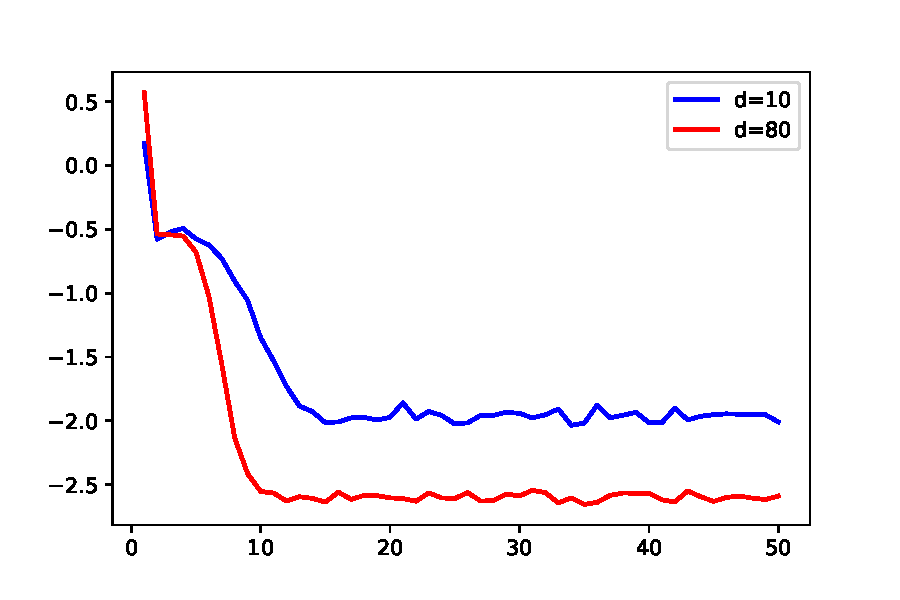
\includegraphics[width=0.45\textwidth]{figures/wdist_bn.pdf}
%      \caption{\footnotesize{\textbf{Gaussian approximation.} The empirical Wasserstein distance (vertical) between the distribution of the network outputs and Gaussian distribution, i.e.   $\log(\mathcal{W}_2(\law(W_\ell H_\ell)),\law(G/\sqrt{n})))$ width $\ell$ (horizontal). See details in Section~\ref{ortho:sec:wasserstein_est}.}}
%      \label{ortho:fig:wasserstein_decay}
%  \end{figure}

\section{The orthogonality and optimization}
\label{ortho:sec:optimization}
In the preceding sections, we elaborated on the theoretical properties of BN networks in controlled settings. 
In this section, we demonstrate the practical applications of our findings. In the first part, we focus on the relationship between depth and orthogonality. Increasing depth drastically slows the training of neural networks with BN. Furthermore, we observe that as depth grows, the training slowdown highly correlates with the orthogonality gap. This observation suggests that SGD needs to orthogonalize deep representations in order to start classification. This intuition leads us to the following question: If orthogonalization is a prerequisite for training, can we save optimization time by starting from orthogonal representations? To test this experimentally, we devised a weight initialization that guarantees orthogonality of representations. Surprisingly, even in a network without BN, our experiments showed that this initialization avoids the training slow down, affirmatively answering the question. 

Throughout the experiments, we use vanilla MLP (without BN) with a width of 800 across all hidden layers, ReLU activation, and used Xavier's method for weights intialization~\citep{glorot2010understanding}. We use SGD with stepsize $0.01$ and batch size $500$ and for training. The learning task is classification with cross entropy loss for CIFAR10 dataset~\citep[][MIT license]{krizhevsky2009learning}. We use PyTorch~\citep[][BSD license]{NEURIPS2019_9015} and Google Colaboratory platform with a single Tesla-P100 GPU with 16GB memory in all the experiments. The reported orthogonality gap is the average of the orthogonality gap of representation in the last layer.


\subsection{Orthogonality correlates with optimization performance}
In the first experiment, we show that the orthogonality of representations at the initialization correlates with optimization speed. For networks with 15, 30, 45, 60, and 75 widths, we register training loss after 30 epochs and compare it with the initial orthogonality gap. Figure~\ref{ortho:fig:slowdown_depth} shows the training loss (blue) and the initial orthogonality gap (red) as a function of depth. We observe that representations are more entangled, i.e., orthogonal, when we increase depth, coinciding with the training slowdown.  Intuitively, the slowdown is due to the additional time SGD must spend to orthogonalize the representations before classification. In the second experiment, we validate this intuitive argument by tracking the orthogonality gap during training. Figure~\ref{ortho:fig:slowdown_training} plots the orthogonality gap of output and training loss for a network with 20 layers. We observe that SGD updates are iteratively orthogonalizing representations, marked by the reduction in the orthogonality gap.

 \begin{figure}[!ht]
     \centering
     \begin{subfigure}[b]{0.4\textwidth}
         \centering
         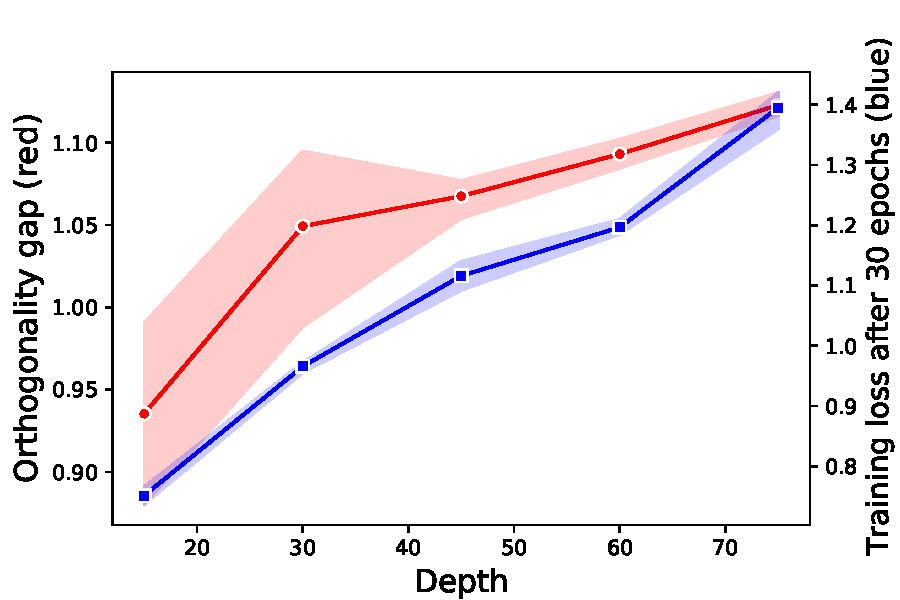
\includegraphics[width=\textwidth]{figures/gaps_loss_depth.pdf}
         \caption{gap and loss vs. depth}
         \label{ortho:fig:slowdown_depth}
     \end{subfigure}
     \begin{subfigure}[b]{0.4\textwidth}
         \centering
         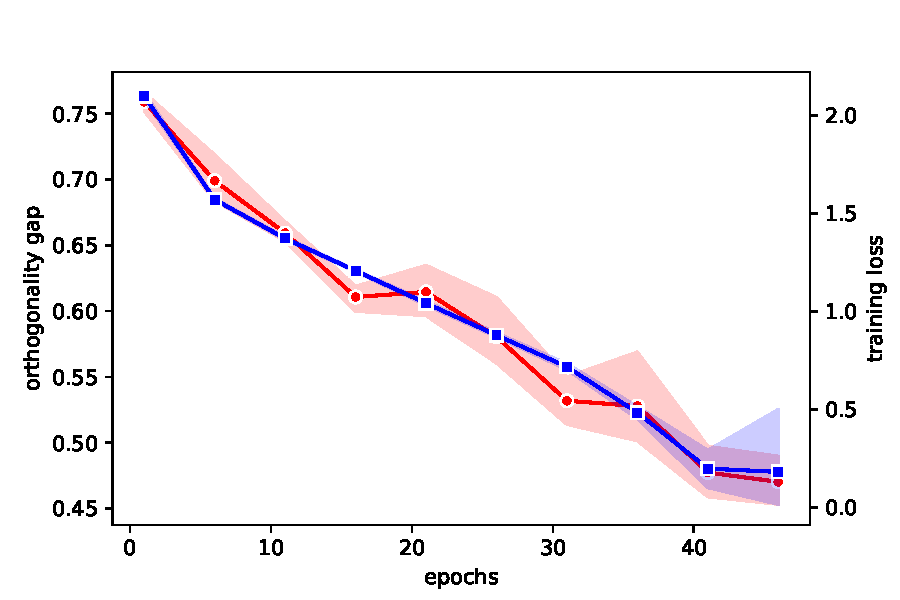
\includegraphics[width=\textwidth]{figures/gaps_training.pdf}
         \caption{gap and loss during training}
         \label{ortho:fig:slowdown_training}
     \end{subfigure}
    \caption{\footnotesize{\textbf{Orthogonality and Optimization} Left: the orthogonality gap at initialization (red, left axis) and the training loss after 30 epochs (blue, right axis) with depth. Right: the orthogonality gap (red, left axis) and  the training loss in each epoch (blue, right axis). Mean and 95\% confidence interval of 4 independent runs. }}
        \label{ortho:fig:slowdown_orthogonality}
\end{figure}


\subsection{Learning with initial orthogonal representations}
We have seen that the slowdown in SGD for deeper networks correlates with the orthogonality gap before training.
Here we show that by preemptively orthogonalizing representations, we avoid the slowdown with depth. While in MPL with linear activations, hidden representations remain orthogonal simply by taking orthogonal matrices as weights~\citep{pennington2018emergence,saxe2013exact}, the same does not hold for networks with non-linear activations, such as ReLU. To enforce the orthogonality in the absence of BN, we introduce a dependency between weights of successive layers that ensures deep representations remain orthogonal. More specifically, we incorporate the SVD decomposition of the hidden representation of each layer into the initialization of the subsequent layer. To emphasis this dependency between layers and to distinguish it from purely orthogonal weight initialization, we refer to this as \emph{iterative orthogonalization}.

We take a large batch of samples $n\geq d$, as the input batch for initialization. Let us assume that weights are initialized up to layer $W_{\ell-1}$. To initialize $W_\ell$, we  compute SVD decomposition of the representations $H_\ell = U_\ell \Sigma_\ell V^\top_\ell$ where matrices $U_\ell \in \R^{d \times d}$ and $V_\ell \in \R^{n \times d}$ are orthogonal. Given this decomposition, we initialize $W_\ell$ by 
\begin{align} \label{ortho:eq:init_w}
    W_\ell = \frac{1}{\| \Sigma_\ell^{\sfrac{1}{2}}\|_F} V_\ell' \Sigma_\ell^{-\sfrac{1}{2}} U_\ell^\top,
\end{align}
where $V'_\ell \in \R^{d\times d}$ is an orthogonal matrix obtained by slicing $V_\ell \in \R^{n\times d}$. Notably, the inverse in the above formula exists when $n$ is sufficiently larger than $d$ \footnote{We may inductively assume that $H_\ell$ is almost orthogonal by the choice of $W_1, \dots, W_{\ell-1}$. Thus, $\Sigma_\ell$ is invertible. }. 
It is easy to check that  $V(W_\ell H_\ell)< V(H_\ell)$ holds for the above initialization (see Section~\ref{ortho:sec:init}), similar to BN. 
%We observed this method effectively orthogonalizes hidden representations when the batch size is sufficiently large. Fig.~\ref{ortho:fig:cifar_orthogonal_a} compares the orthogonality gap of the representations for this initialization method with a standard initialization. 
By enforcing the orthogonality, this initialization significantly alleviates the slow down of training with depth (see Fig.~\ref{ortho:fig:cifar_orthogonal}), with no need for BN. This initialization is not limited to MLPs. In Section~\ref{ortho:sec:bnreplace}, we compare iterative orthogonalization with a BN-replacement method recently proposed by \cite{brock2021high}.  
% In Section~\ref{ortho:sec:experiments}, we propose a similar SVD-based initialization for convolutional networks that effectively accelerates the training of deep convolutional networks.  

 \begin{figure}[!ht]
     \centering
         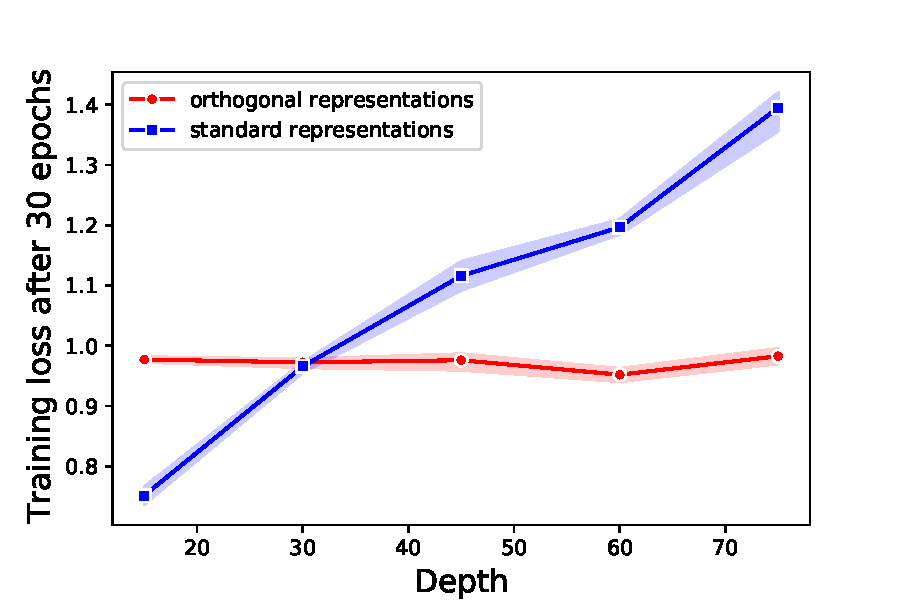
\includegraphics[width=0.55\textwidth]{figures/training_orth.pdf}
    \caption{\footnotesize{\textbf{Iterative orthogonalization.} Horizontal axis: depth. Vertical axis: the training loss after 30 epochs for Xavier's initialization (blue), our initialization (red). Mean and 95\% confidence interval of 4 independent runs.}}
        \label{ortho:fig:cifar_orthogonal}
\end{figure}



\section{Discussion}
To recap, we proved the recurrence of random linear transformations and BN orthogonalizes samples. Our experiments underline practical applications of this theoretical finding: starting from orthogonal representations effectively avoids the training slowdown with depth for MLPs. Based on our experimental observations, a proper initialization ensuring the orthogonality of hidden representations may replace BN in neural architectures. This future research direction has the potentials to boost the training of deep neural networks and change benchmarks in deep learning.


Although our theoretical bounds hold for MLPs with linear activations, our experiments confirm similar orthogonal stability for various neural architectures. 
%  Figure~\ref{ortho:fig:relu_convnet} demonstrates this stability for MLPs with ReLU activations and a convolutional networks. This plot compares the evolution of the orthogonality gap, through layers, for BN networks with vanilla networks. For vanilla networks, we observe that the gap increases with depth. On the contrary, the gap decreases by adding BN layers and stabilizes at a term that is constant with regard to depth. Based on our observations, we conjecture that hidden representations of modern BN networks obey similar stability. A more formal statement of the conjecture is presented in Section~\ref{ortho:sec:activations}. 

\cite{lubana2021beyond} experimentally compares properties of different normalization techniques including layer normalization (LN)~\citep{ba2016layer}. According to this study,  LN does not necessarily orthogonalize the outputs of deep neural networks. Hence, more theoretical studies are required to understand the essence of different normalization techniques in deep learning.
% \section*{Acknowledgements}
%  We thank Gideon Dresdner, Vincent Fortuin, and Ragnar Groot Koerkamp for their helpful comments and discussions. This work was funded in part by the French government under management of Agence Nationale de la Recherche as part of the “Investissements d’avenir” program, reference ANR-19-P3IA-0001(PRAIRIE 3IA Institute). We also acknowledge support from the European Research Council (grant SEQUOIA 724063). 


% \end{document}

% !TEX root = ../thesis-index.tex


\chapter{Briding mean field and finite width analysis}\label{ch:bn_MF}


There is a growing demand for a theoretical understanding of neural networks to improve their safety, robustness, computational and statistical effectiveness. Originating in statistical mechanics for investigating complex systems with interacting particles, this theory has been repurposed in recent years for exploring neural network dynamics under the regime of infinite width. By going beyond the microscopic changes of individual neurons, mean field analysis has revealed the collective neuronal behaviors that emerge at initialization~\cite{pennington2018emergence,yang2018a,pennington2017nonlinear}, throughout training \cite{jacot2018neural,bach2021gradient,lee2019wide}, and after training \cite{chizat2020implicit,ba2019generalization}.

In this chapter, we delve into the role of mean field theory at initialization when network weights are allocated randomly. Pioneering works by~\citet{pmlrv9glorot10a} and~\citet{saxe2013exact} underscored the impact of initialization on training, paving the way for mean field theory to uncover a wealth of insights. Examples include identifying connections between wide neural networks and Gaussian processes~\cite{neal2012bayesian,matthews2018gaussian,jacot2018neural}, examining the concentration of singular values of input-output Jacobians~\cite{pennington2018emergence,feng2022rank}, and designing activation functions~\cite{klambauer2017self,ramachandran2017searching,li2022neural}. Remarkably,~\citet{xiao2018dynamical} introduced an initialization scheme capable of training convolutional networks comprising $10000$ layers.

A common thread among these studies is the dynamics of inner products between hidden representations, encoded in their Gram matrix. Mean field theory models these dynamics via a difference equation derived from the infinite-width limit of the network. However, mean field analysis is inherently prone to approximation errors when dealing with networks of finite width. As \citet{matthews2018gaussian} observed, this error grows with depth, ultimately leading to vacuous error bounds in the infinite depth limit. To tackle this issue,  they propose to increase the network width proportional to depth. This idea is echoed in other studies which propose maintaining a constant ratio between depth and width~\cite{hanin2019finite,li2021future}, a regime in which~\citet{hanin2022correlation} confirmed a constant concentration bound for mean field estimates.

Can we achieve a bounded mean field error when the width is finite? We answer this question affirmatively for MLPs that are endowed with batch normalization. In particular, we show that under some technical assumption on the underlying dynamics (as formally expressed in Theorem~\ref{MF:thm:concentration}), the mean field estimation error for Gram matrices remains bounded at infinite depth. Specifically, we demonstrate that this error is limited by $\text{width}^{-1/2}$ with high probability. This contrasts with the vacuous concentration bounds at infinite depth observed in the absence of normalization~\cite{li2022neural}. Our results highlight the importance of existing mean field analyses of batch normalization by~\citet{yang2018a}, and demonstrate their high accuracy in the finite width scenarios that are relevant for practical applications.\footnote{Codes available at \url{https://github.com/ajoudaki/mean field-normalization}.}


\section{Related works}
Numerous studies~\cite{saxe2013exact,feng2022rank,yang2018a} have provided valuable insights into training neural networks by studying input-output Jacobians of neural networks with and without normalization at initialization. For example, ~\citet{feng2022rank} have shown that the rank of the input-output Jacobian of neural networks without normalization at initialization diminishes exponentially with depth, while ~\citet{yang2018a} have shown that batch normalization avoids this exponential diminishing. 

The spectrum of Jacobians is intimately related to the spectra of Gram matrices. 
A Gram matrix (G-matrix) contains inner products of samples within a batch (\eqref{MF:eq:gram_matrix}). Thus, a degenerate G-matrix for the penultimate layer implies that the outputs are insensitive to the inputs~\cite{feng2022rank,li2022neural}.  
Rank collapse in the last hidden layer occurs in various neural network architectures, including MLPs~\cite{saxe2013exact}, convolutional networks~\cite{daneshmand2020batch}, and transformers~\cite{dong2021attention}, and leads to ill-conditioning of the input-output Jacobian, which slows training~\cite{daneshmand2021batch,pennington2018emergence,yang2018a}. ~\citet{saxe2013exact} have shown that avoiding rank collapse can accelerate the training of deep linear networks, making it a focus of theoretical and experimental research~\cite{pennington2018emergence,daneshmand2020batch,daneshmand2021batch}.


A recent line of research~\cite{daneshmand2020batch} postulates that batch normalization can enhance the training of deep neural nets by avoiding the rank collapse. This claim has been supported by empirical evidence~\cite{yang2018a,daneshmand2020batch}, as well as theoretical studies for neural networks with infinite widths~\cite{yang2018a} and linear activation~\cite{daneshmand2021batch}. It has been shown that batch normalization prevents degenerate representations at initialization~\cite{daneshmand2020batch}, and orthogonalizes representations~\cite{daneshmand2021batch}. However, these results are limited to linear activations.
The present study extends these findings to neural networks with finite widths and non-linear activations, under an assumption from Markov chain theory. 


\section{Problem settings and background}

\paragraph{Notation and terminology.}
$I_n$ denotes the identity matrix of size $n\times n$ and $1_n$ denotes the all ones vector in $\R^n$.  
$\otimes$ refers to Kronecker product. $\mu_X$ refers to the probability measure of the random variable $X$. We use $f\lesssim g, g \gtrsim f$ and $f = \O(g)$ to denote the existence of an absolute constant $c$ such that $f\le c\; g.$ 
$\norm{v}$ for a vector $v$ denotes the $L^2$ norm.
$\norm{C}$ for matrix $C$ denotes the $L^2$ operator norm $\norm{C}=\sup_{x\in\R^n}\norm{C x}/\norm{x}$, $\norm{C}_F$ denotes the Frobenius norm. We use $\kappa(C)$ to denote the ratio of largest to smallest eigenvalue. Both $h_{r\cdot}$ and $\row_r(h)$ denote row-vector representation of the $r$-th row of $h.$ Finally, $X\sim \Normal(\mu,\sigma^2)^{n\times m}$ denotes $X\in\R^{n\times m}$ is a Gaussian matrix whose elements are drawn \iid from $\Normal(\mu,\sigma^2).$ 

\paragraph{Setup.}
Let $h_\ell\in \R^{d\times n}$ denote the hidden representation at layer $\ell$, where $n$ corresponds to the size of the mini-batch, and $d$ denotes the width of the network that is kept constant across all layers. The sequence  $\{h_\ell\}$ is a Markov chain as
\begin{align}\label{MF:eq:chain}
h_{\ell+1}:=W_\ell \act\circ\BN(h_\ell), && W_\ell\sim\Normal(0,\nfrac1d)^{d\times d},
\end{align}
where $h_0\in\R^{d\times n}$ is the input batch, $\act$ is the element-wise activation function, and $\BN$ is the batch normalization \cite{ioffe2015batch}, which applies row-wise centering and scaling by standard deviation:
\begin{align*}
\BN(x) = \frac{x - \text{mean}(x)}{\sqrt{\text{Var}(x)}}, && \forall r: \row_r(\BN(h)) = \BN(\row_r(h)).
\end{align*} 
  

\section{Mean field models and fixed-point analyses}
\subsection{Mean field Gram dynamics}
The Gram matrix $G_\ell$ is defined as the matrix of inner products of hidden representations at layer $\ell$ as seen in the equation below:
\begin{align}\label{MF:eq:gram_matrix}
G_\ell := \frac1d (\act\circ\BN(h_\ell))(\act\circ\BN(h_\ell))^{\top}.
\end{align}
Understanding the dynamics of $G_\ell$ is a significant challenge in deep learning theory, and has been the subject of several studies \cite{yang2018a,pennington2018emergence,pennington2017nonlinear}. Due to the randomness of weights, determining the trajectory of this random process proves to be arduous. By tending width $d$ to infinity, i.e., the mean field regime, we can approximate these stochastic dynamics with a deterministic dynamics as below:
\begin{align}\label{MF:eq:MF_recurrence}
\overline{G}_{\ell+1} = \E_{h\sim \Normal(0,\overline{G}_\ell)}\left[\act\left(\frac{ \sqrt{n} M h}{\| Mh\|}\right)^{\otimes 2}\right],
\end{align}
Where $\overline{G}_{0} = G_0$ serves as the input G-matrix and ${M = I_n - \frac1n1_n^{\otimes 2}}$ applies mean reduction on the preactivations. The mean field approach in this context assists in elucidating the analysis of Gram matrices.

\subsection{Fixed point analysis for infinitely deep and wide Networks}
The fixed points of the mean field dynamics, as expressed in ~\eqref{MF:eq:MF_recurrence} may help elucidate the properties of $\overline{G}_{\ell}$ as $\ell \to \infty$. 
\citet{yang2018a} provide a comprehensive characterization of these fixed-points, denoted by $\C$, for neural networks with batch normalization. For networks with linear activations, \citet{yang2018a} establish a global convergence to these well-conditioned fixed-points. While they empirically observe convergence to these well-conditioned fixed-point for networks with non-linear activations, that is not established theoretically. In other words, it is challenging to describe the properties of $\overline{G}_\ell$ for finite width and depth, and it is unclear how the fixed-point Gram matrix $\C$ can inform us about~$G_\ell$.

\subsection{An observation}
Through an empirical observation we can demonstrate that $\C$ may not always provide an accurate estimate for $G_\ell$. We observe that for a network without batch normalization and linear activations (when $\act\circ\BN=identity$ in~\eqref{MF:eq:chain}), the Frobenius distance between $G_\ell$ and $\C$ increases with $\ell$. In contrast, $G_\ell$ converges to a neighborhood of $\C$ when the network includes batch normalization layers. These observations suggest that the mean field estimate $\C$ from \citet{yang2018a} accurately represents $G_\ell$ when batch normalization is present.
  

 
\begin{figure}
    \centering
    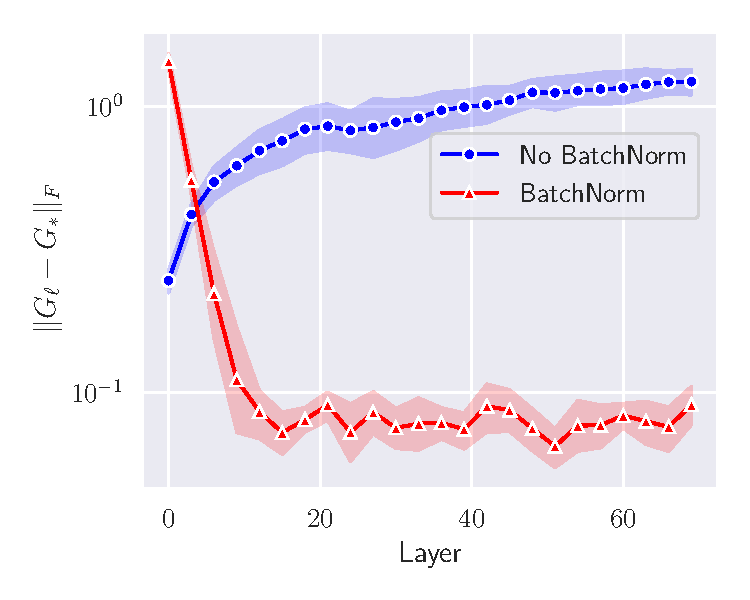
\includegraphics[width=0.45\textwidth]{figures/bn_without.pdf}
    \vspace{-.5cm}
    \caption{\textit{Mean field error amplification with(out) batch-normalization.} The horizontal axis represents the number of layers $\ell$ (linear), while the vertical axis (log-scale) shows $\|G_\ell- G_*\|_F$, for networks with $n=5, d=1000$. The traces show mean and shades indicate $90\%$ confidence intervals over $10$ independent simulations. }
    \label{MF:fig:rapidly_mixing}
\end{figure}



\subsection{The challenge of depth for mean field theory}
Mean field analysis suffers from a systematic estimation error that increases with depth. Assuming that $\overline{G}_0= G_0$, then an error of $O(d^{-1/2})$ is observed between $\overline{G}_1$ and $G_1$ due to the concentration of empirical covariance. Consequently, the mean field dynamics in \eqref{MF:eq:MF_recurrence} incur an error of $O(d^{-1/2})$ at each layer~\cite{li2022neural}. As depth $\ell$ grows, these errors are amplified, and the bounds on $\| G_\ell - \overline{G}_\ell\|_F $ become vacuous, thus raising questions about the practical applicability of these fixed-point analyses when width is finite. 

Several studies strive to refine the mean field model to enhance its predictive accuracy ~\cite{matthews2018gaussian,hanin2019finite,li2022neural}. \citet{li2022neural} propose using a stochastic differential equation to model the layer-wise $O(d^{-1/2})$ estimation error for mean field Gram dynamics. This approach allows for accurate predictions of Gram dynamics for MLPs with activation functions but only in the infinite-width-and-depth regime. Our observations, however, suggest that for networks with batch normalization, the deterministic model of Gram matrices provides a surprisingly accurate estimate.

\citet{daneshmand2021batch} established this observation for multilayer perceptrons (MLPs) with batch normalization (BN) and linear activations, subject to specific conditions. They demonstrated that as $\ell$ increases, batch normalization progressively aligns the Gram matrices $G_\ell$ with the identity matrix, which coincides with $G_*$ for such networks \cite{yang2018a}. \citet{yang2018a} further proved a concentration bound for $\|G_\ell - G_*\|_F$ in networks with batch normalization and linear activations. However, both these findings are limited to linear activations. Our objective is to extend these results to networks incorporating non-linear activations.




\section{Concentration bounds for Mean field Predictions with Batch Normalization}


\subsection{Geometric ergodic assumption} 
The chain of hidden representations obeys a non-linear stochastic recurrence. Despite this non-linearity, the distribution associated with the representation obeys a linear fixed-point iteration determined by the Markov kernel $K$ associated with the chain $h_\ell$. The distribution of $h_\ell$, denoted by $\mu_{\ell},$ obeys 
\begin{align} \label{MF:eq:dist_recurrence}
    \mu_{\ell+1} = T(\mu_{\ell}), \quad T(\mu) := \int K(x,y) d\mu(y).
\end{align}
The fixed-points of the above equation are invariant distributions of the chain, which we denote by $\mu_*$.  Recall that the total variation for distributions over $d\times n$ matrices can be defined as $\tv{X}{Y}:=\sup_{A\subseteq\R^{d\times n}} |\mu_X(A)-\mu_Y(A)|.$
Notably, the above recurrence is non-expansive in total variation, hence $\|\mu_\ell - \mu_*\|_{tv} \leq \| \mu_{\ell-1} - \mu_* \|_{tv}$ holds for all~$\ell$.
However, we assume the chain obeys a strong property ensuring the convergence to a unique invariant distribution. 


\begin{assumption}[Geometric ergodicity]\label{MF:ass:rapid_mixing}
 We assume the chain of hidden representations admits a unique invariant distribution. Furthermore, there is constant $\alpha$ ($\alpha>0$) such that
\begin{align*}
\tv{\ell}{*} \le (1-\alpha)^\ell \tv{0}{*},
\end{align*}
holds almost surely for all $h_0$.
\end{assumption}

The geometric ergodic property is established for various Markov chains, such as the Gibbs sampler, state-space models~\cite{eberle2009markov}, hierarchical Poisson models~\cite{rosenthal1995minorization}, and Markov chain Monte Carlo samplers~\cite{jones2001honest}. ~\citet{doeblin1938deux} provides weak conditions that ensure geometric ergodicity. Doeblin's condition holds when the Markov chain can explore the entire state space~\cite{eberle2009markov}. This condition may hold under weak assumption on the input matrix for the chain of hidden representations.  
In particular, when $h_\ell$ has full rank, the Gaussian product $W_\ell h_\ell$ may explore the entire $\R^{d\times n}$.  



\subsection{Main result}
The next theorem proves fixed-point $\C$ provides an estimate for Gram matrices of sufficiently deep neural networks with a finite width. 

\begin{theorem}[BN-MLP Concentration]\label{MF:thm:concentration}
Assume the Markov chain of representations $\{h_\ell\}$ obeys Assumption~\ref{MF:ass:rapid_mixing} with $\alpha >0,$ and has non-degenerate fixed-point $G_*.$ If the activation $\act$ is uniformly bounded $|\act(x)| = O(|x|),$ then Gram matrix deviation $\|G_*-G_\ell\|_F$ is bounded by
\begin{align}
\kappa(G_*) O\left((1-\alpha)^{\frac{\ell}{2}}+ \frac{n}{\sqrt{d}}\alpha^{-\frac12}\ln^{\frac12}(\frac{d}{n}) \right),
\end{align}
with high probability in $d$ and $\ell.$
\end{theorem}

Theorem~\ref{MF:thm:concentration} quantifies the accuracy of our mean field predictions in terms of batch size, width, depth, and conditioning of $G_*$. Notably, almost all commonly used activations, e.g., ReLU and hyperbolic tangent, satisfy the uniform bounded condition $|\act(x)|=O(|x|).$ Under Assumption~\ref{MF:ass:rapid_mixing}, this theorem proves the fixed-point Gram matrix $G_*$ accurately estimates $G_\ell$ for a sufficiently large $\ell$. According to this theorem, $\| G_\ell - \C \|_F$ decays with depth at an exponential rate. Thus, approximately after a logarithmic number of layers $\ell\approx \log(\text{width}/\text{batch-size}),$ the term $O(n /\sqrt{d})$ dominates the distance.

Remarkably, this is a considerable improvement compared to the concentration bounds for neural networks without batch normalization that become vacuous  as the depth increases~\cite{hanin2019finite,hanin2022correlation}. The established bound in the last theorem holds jointly for all $\ell$ in that we do not need to apply union bound. 


Let us remark that if the fixed-point Gram matrix is degenerate, i.e., if $\kappa(G_*)$ is unbounded, the bound of the Theorem becomes vacuous. Therefore, Theorem~\ref{MF:thm:concentration} reinforces the necessity for a well-conditioned fixed-point for the mean field errors to remain within bounds. As long as the fixed-point Gram is well-conditioned, the Gram matrices $G_\ell$'s stay within an $O(\text{batch}/\text{width}^{1/2})$ proximity with constant probability.

When contrasting Theorem~\ref{MF:thm:concentration} with the activation shaping approach by~\citet{li2022neural}, we observe that while activation shaping necessitates solving a stochastic differential equation to track the dynamics of the Gram matrix, BN-MLP relies solely on the mean field prediction $\C,$ which can be computed in closed-form~\citet{yang2018a}.


\paragraph{Proof Sketch of Theorem~\ref{MF:thm:concentration}.}
We first construct an approximate invariant distribution, associated with $T$ as defined in \eqref{MF:eq:dist_recurrence}. For the construction of such distribution, we utilize the mean field Gram matrix to form an input $\hat h\in\R^{d\times n},$ with rows drawn i.i.d. from $\row_r(\hat h)\sim \Normal(0,\C)$. The next lemma proves that the law of $\hat h,$ denoted by $\hat \mu,$ does not significantly change under $T.$

\begin{lemma}\label{MF:lem:tv_one_step}
Assuming uniformly bounded activation ${|\act(x)| = O(|x|)},$ we have
\begin{align}
\| T(\hat \mu)- \hat \mu \|_{tv}\lesssim \norm{G_*^{-1}} \frac{n^2}{d}\ln(d/n).
\end{align}
\end{lemma}

The proof of the last lemma is based on the fixed-point property of $\C$ (see Appendix for the detailed proof). Using the last lemma together with
Assumption~\ref{MF:ass:rapid_mixing}, we prove that~$\hat \mu$ is in a $tv$-ball around the invariant distribution $\mu_*$. Under this assumption, we have 
\begin{equation}
\begin{aligned}
    \| T(\hat \mu)-T(\mu_*)\|_{tv} &= \|T(\hat \mu)-\mu_*\|_{tv} \\
    & \leq (1-\alpha) \|\hat \mu- \mu_*\|_{tv},
\end{aligned}
\end{equation}
where we used the invariant property of $\mu_*$ in the above equation. 
Using triangular inequality, we get 
\begin{equation}
\begin{aligned}
    \| T(\hat \mu) - \hat \mu\|_{tv} & = \| T(\hat \mu) -\mu_* +\mu_*- \hat \mu\|_{tv} \\ 
    & \geq \| \mu_*- \hat \mu\|_{tv} -\|T(\hat \mu) - \mu_*\|_{tv} \\ 
    & \geq \alpha \| \hat\mu-\mu_* \|_{tv}.
\end{aligned}
\end{equation}
Plugging the bound from the last lemma into the above inequality concludes $\hat \mu$ lies within a radius $n^2\|G_*^{-1}\|/d\alpha$ of $\mu_*$. This concludes the proof: Since the chain is geometric ergodic, the distribution $\mu_\ell$ converges to an $tv$-ball around $\hat \mu$ at an exponential rate. This allows us to characterize the moments of $ \mu_\ell$ using those of $\hat \mu$. 

\subsection{Validation of main theoretical results}
Our principal finding suggests a link between the Gram matrices of hidden representations with independent weights. Assuming $\kappa(G_*)=O(1)$ this is captured by the relation:
\begin{equation}
\|G_\ell - G_*\|_F =O\left((1-\alpha)^{\ell/2} + \frac{n}{\sqrt{d}}\right).
\end{equation}

We test this relationship by numerically estimating $G_*$ by tending $d$ and $\ell$ to sufficiently large values. We then plot the left-hand side of the above equation versus depth, width, and batch size in the following figures. These plots illustrate how the difference in Gram matrices changes with respect to depth, width, and batch size. This supports our theoretical results and showcases their potential implications for practical settings. 
\begin{figure}[ht]
\centering
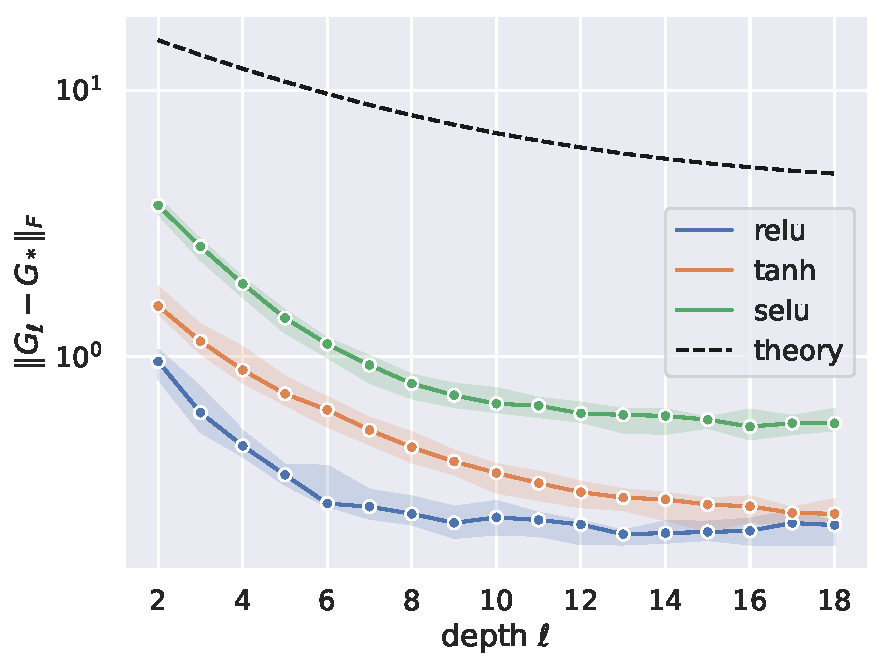
\includegraphics[width=.45\textwidth]{figures/Gram_diff_vs_l.pdf}
\vspace{-.4cm}
\caption{$\|G_\ell - G_*\|_F$ vs. depth, $\ell = 1,2,...,20,$ with a fixed width of $d=1000$ and a batch size of $n=10$. The dashed line shows the theoretical upper bound of Theorem~\ref{MF:thm:concentration}.}
\label{MF:fig:Gram_vs_depth}
\end{figure}
\begin{figure}[ht]
\centering
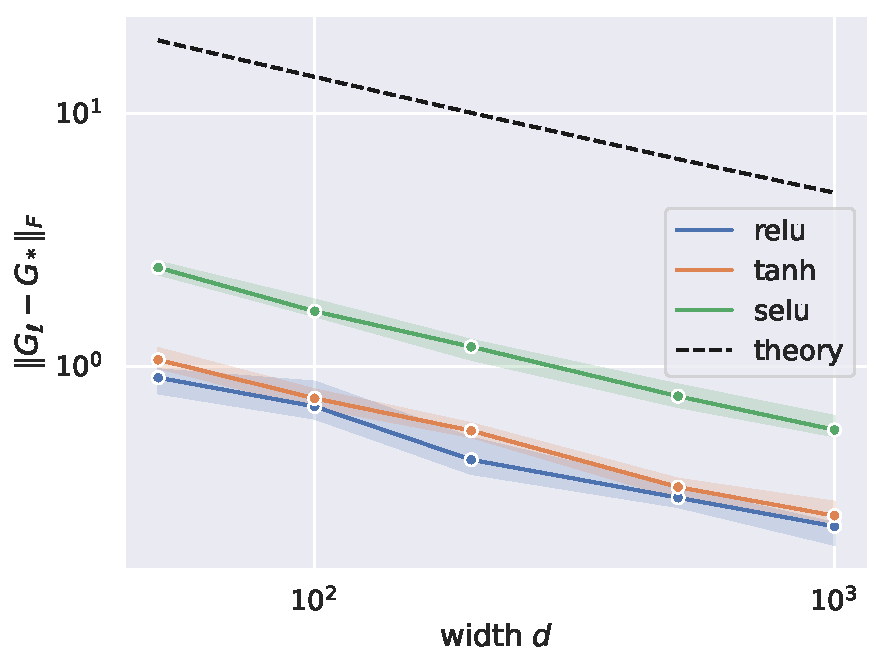
\includegraphics[width=.45\textwidth]{figures/Gram_diff_vs_d.pdf}
\vspace{-.4cm}
\caption{$\|G_\ell - G_*\|_F$ vs. width, $d=50,100,200,500,1000$, with a fixed depth of $\ell=20$ and a batch size of $n=10.$ The second term $O(n/\sqrt{d})$ is always dominant, as demonstrated in the following log-log plot.}
\label{MF:fig:Gram_vs_width}
\end{figure}

\begin{figure}[ht]
\centering
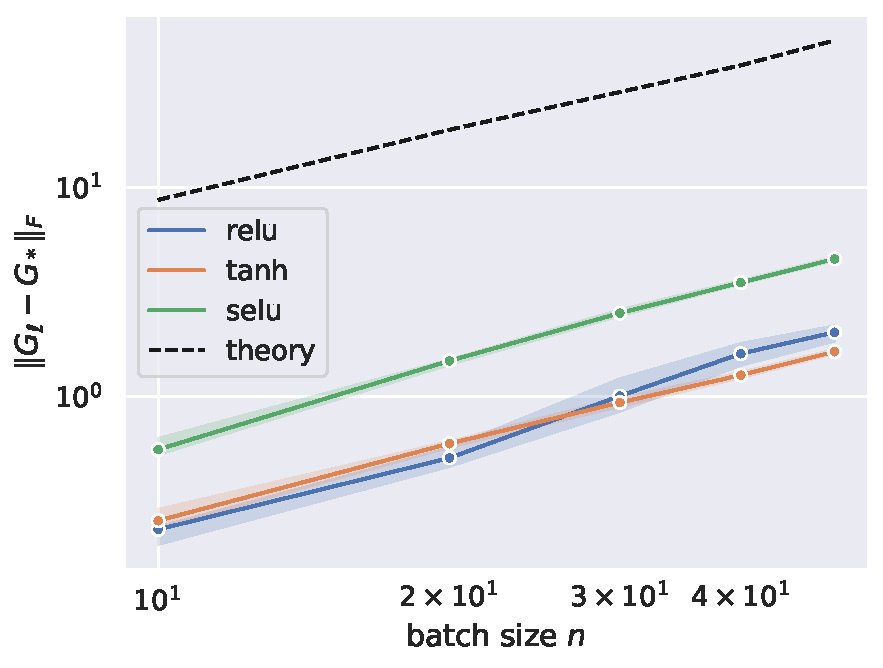
\includegraphics[width=.45\textwidth]{figures/Gram_diff_vs_n.pdf}
\vspace{-.4cm}
\caption{$\|G_\ell - G_*\|_F$ vs. batch size, with a fixed width of $d=1000$ and a depth of $\ell=20,$ and varying batch sizes of $n=10,20,30,40,50.$ Dashed line shows upper bound given in Theorem~\ref{MF:thm:concentration}.}
\label{MF:fig:Gram_vs_n}
\end{figure}

You can find the detailed proofs in Chapter~\ref{ch:bn_MF:proofs}.


% \section{Applications}\label{MF:sec:validations}
% The spectral analysis of Gram matrices plays a central role in numerous theoretical and practical machine learning studies. For instance, these matrices are used to design activations, contributing to improved conditioning~\cite{klambauer2017self}, and to create novel initialization schemes for training convolutional networks with $10000$ layers~\cite{xiao2018dynamical}. One line of research links the enhanced performance of neural networks incorporating batch normalization to the well-conditioning of Gram matrices $G_\ell$ \cite{yang2018a,daneshmand2020batch,daneshmand2021batch}. Since the existing literature often uses mean field approximations, we can leverage Theorem~\ref{MF:thm:concentration} to evaluate accuracy of these approximations for finite width and depth settings.

% \subsection{Well-conditioning with batch normalization}

% Empirical studies suggest that the conditioning of Gram matrices, $G_\ell$, has a substantial impact on the training of deep neural networks \cite{xiao2018dynamical,pennington2018emergence,li2022neural,daneshmand2020batch}. 
% % Observations show that initializing the optimization process from well-conditioned Gram matrices leads to a faster convergence for stochastic gradient descent. 
% Experimental evidence suggests that batch normalization can ensure the good conditioning of $G_\ell$~\cite{yang2018a,daneshmand2021batch}, thereby enhancing the training of deep neural networks.

% In a seminal study, \citet{yang2018a} study the fixed points of the mean field equation of an MLP with batch normalization. In particular, they demonstrate that one fixed point $G_*$ follows the following form:
% \begin{align}\label{MF:eq:stable_G_symmetric}
% \C = b^*\left( (1-c^*)I_n + c^* \1_{n\times n}\right),
% \end{align}
% where $c^*$ and $b^*$ are constants determined by the activation function. Given the distinctive construction for $\C,$ we can deduce the structure of its eigenvalues, with the largest eigenvalue being ${\lambda^*_1=(1+(n-1)c^* )b^*},$ and all others being equal to $\lambda^*_2=\dots=\lambda^*_n = b^*(1-c^*).$ 

% While the mean field analysis discussed above holds for infinitely wide and deep neural networks, it is possible to utilize Theorem~\ref{MF:thm:concentration} to link the spectrum of $\C$ with the spectra of Gram matrices for networks of finite width. Using the Hoffman-Wielandt inequality~\cite{hoffman2003variation}, we can calculate a bound on the deviation of the spectrum of $G_\ell$ from $G_*,$ using the bound on their Frobenius distance.


% \begin{corollary}[Spectral concentration]\label{MF:cor:spectrum}
% In the same settings as Theorem~\ref{MF:thm:concentration}, let $\lambda_i$ and $\lambda_i^*$ denote eigenvalues of $G_\ell$ and $G_*$ respectively in a descending order. Assuming that ${\kappa(G_*) = O(1)}$, the deviation of their spectra $\sqrt{\Sigma_{i=1}^n(\lambda_i-\lambda_i^*)^2}$ is bounded by
% \begin{align}
% O\left((1-\alpha)^{\frac{\ell}{2}}+ \frac{n}{\sqrt{d}}\alpha^{-\frac12}\ln^{\frac12}(\frac{d}{n}) \right),
% \end{align}
% with high probability in $d$ and $\ell.$
% \end{corollary}

% Substituting the spectrum of $\C$ characterized by \citet{yang2018a} into the above concentration, we can estimate the spectra of Gram matrices $G_\ell$, encapsulated in the following proposition.

% \begin{proposition}\label{MF:cor:ESD_spect}
% In the same setting as Theorem~\ref{MF:thm:concentration}, assuming $G_*$ complies with equation~\ref{MF:eq:stable_G_symmetric}, then for a sufficiently deep layer $\ell$, $n-O(1)$ eigenvalues of $G_\ell$ are within $O(\sqrt{n/d})$ range of $b^* (1-c^*)$ with high probability in $d$.
% \end{proposition}

% The above proposition provides a characterization for the ``bulk'' of eigenvalues of~$G_\ell$, by postulating that majority of eigenvalues of $G_\ell$ are concentrated around some absolute constant, up to $\sqrt{n/d}$ range. Interestingly, this bears resemblance to the Marchenko-Pastur~\cite{pastur1967distribution} law on the eigenvalue distribution of Wishart matrices of comparable size. We observe empirically that the singular values of $h_\ell,$ which are square root of eigenvalues of $G_\ell,$ accurately follow the Marchenko-Pastur distribution with $\gamma={n/d}$, as depicted in Figure~\ref{MF:fig:MP_ESD}. Our empirical evaluations show that this distribution accurately predicts singular values of hidden representations for commonly used activation functions with various widths (see Appendix for empirical evidence).

%  \begin{figure}[ht]
%  \centering
%  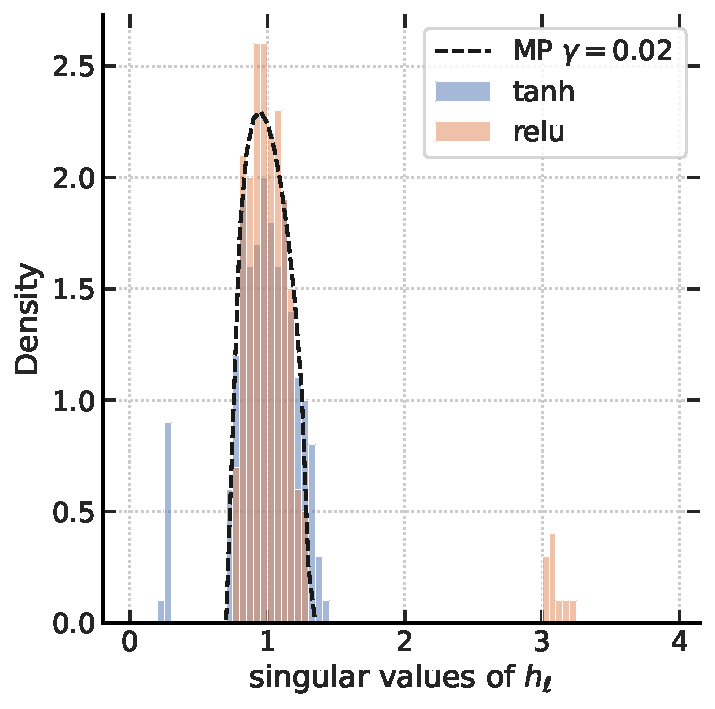
\includegraphics[width=0.4\textwidth]{figures/singular_values_relu_tanh.pdf}
%  \vspace{-.5cm}
%  \caption{BN-MLP with $n=20,d=1000$, $\ell=20$: histogram shows the empirical distribution of singular values of $h_\ell,$ for $\act=\relu$ and $\act=\tanh.$ The black curve marks the Marchenko-Pastur distribution with $\gamma={n/d}=0.02.$ The singular values are normalized by their medians in this plot to be aligned at $1.0$}
%  \label{MF:fig:MP_ESD}
% \end{figure}

% It is worth noting that only the $O(1)$ singular values are influenced by the activation function, while the remaining $n-O(1)$ exhibit a universal behavior. For example in the case of $\act=\relu,$ a single large eigenvalue is associated with the $\1_n$ direction, owing to the non-negativity of $\relu$ outputs. 

% \subsection{Influence of Gram matrix conditioning on training}
% Having explored the influence of batch normalization on the spectra of the Gram matrices, we now turn our attention to its effects during training.  
% It has been hypothesized that batch normalization facilitates the training of neural networks at the initialization stage by ensuring the deep representations are biased towards a uniform prior on class probabilities~\cite{daneshmand2021batch}. In contrast, it has been reported poor Gram matrix conditioning in standard MLP leads to the gradual alignment of deep hidden layers, thereby resulting in highly similar logits across different samples in the batch~\cite{daneshmand2020batch,daneshmand2021batch}. Batch normalization effectively resolves this issue, ensuring a more efficient learning process for the network. While our theoretical studies are limited to initialization, we can empirically explore conditioning of Gram matrix during training. 

% % \paragraph{Gram matrix conditioning during training}
% We examined a standard MLP setup consisting of 10 layers ($L=10$) and a width of 1000 ($d=1000$). We trained this network on mini-batches of size 128 ($n=128$) using the CIFAR100 dataset for 50 epochs, using SGD with a learning rate of $0.001$. This process was carried out on MLP configurations both with and without batch normalization.

% We present the distributions of log-eigenvalues for the penultimate Gram matrix, represented by $\log(\lambda_i(G_L))$, during training in Figure~\ref{MF:fig:training_eigenvals}. It is noteworthy that the eigenvalues of the penultimate Gram matrix for the MLP with batch normalization are more concentrated around their mean than their counterparts in the MLP without batch normalization. This suggests a collapse in class representations in the absence of normalization. 

% To further investigate class representations, we calculated the frequency of each class in the predictions at different training stages. We quantified the entropy of the predicted class probabilities, computed as ${\sum_{i=1}^C p_i \log_2(p_i)}$. In this equation, ${p_c := \frac1N\#\{i\le N: \tilde y_i= c\}}$ designates the proportions of predictions for class $c$, and $\tilde y_i$ represents the prediction for sample $i.$ Observe that a uniform distribution $p_1=\dots = p_C = 1/C,$ leads to the highest entropy $O(\log_2(C))$.

% As illustrated in Figure~\ref{MF:fig:class_entropy}, the MLP with batch normalization closely approximates this uniform prior at initialization. In contrast, the MLP without normalization exhibits a significantly lower initial class entropy. For a balanced dataset like CIFAR100, an optimal model should have a class entropy of approximately $\log_2(100)\approx 6.64$, reflecting a uniform distribution over classes. Hence, batch normalization biases the initial predictions towards a uniform distribution on the labels. The observed discrepancy in Figure~\ref{MF:fig:class_entropy} may thus be related to the accelerated convergence of training loss as depicted in Figure~\ref{MF:fig:training_loss}. 

% The empirical evidence presented here suggests that while Theorem~\ref{MF:thm:concentration} was proven for initialization, Gram matrices of MLP with batch normalization remain well-conditioned during the entire training process. 



% \begin{figure}[ht]
% \centering
% 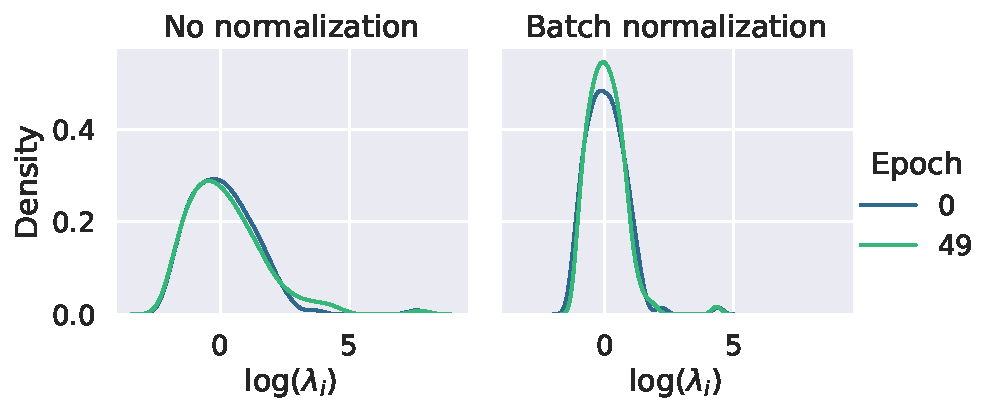
\includegraphics[width=.5\textwidth]{figures/gram_eigenvalues_plot.pdf}
% \vspace{-.8cm}
% \caption{Distribution of log-eigenvalues of penultimate Gram matrix, $\log(\lambda_i(G_L))$ at initialization (epoch $0$) and at the end of training (epoch $49$).}
% \label{MF:fig:training_eigenvals}
% \end{figure}

% \begin{figure}[ht]
% \centering
% 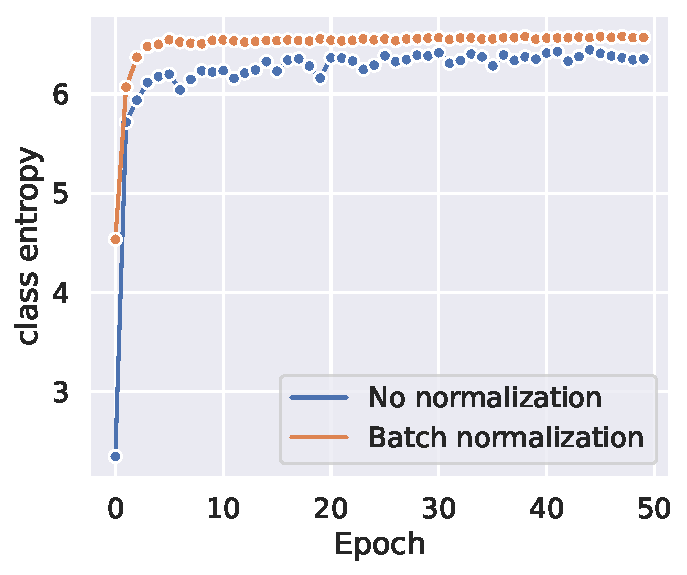
\includegraphics[width=.4\textwidth]{figures/class_entropy.pdf}
% \vspace{-.5cm}
% \caption{Predicted class entropy of MLP with (orange) and without (blue) batch normalization. }
% \label{MF:fig:class_entropy}
% \end{figure}

% \begin{figure}[ht]
% \centering
% 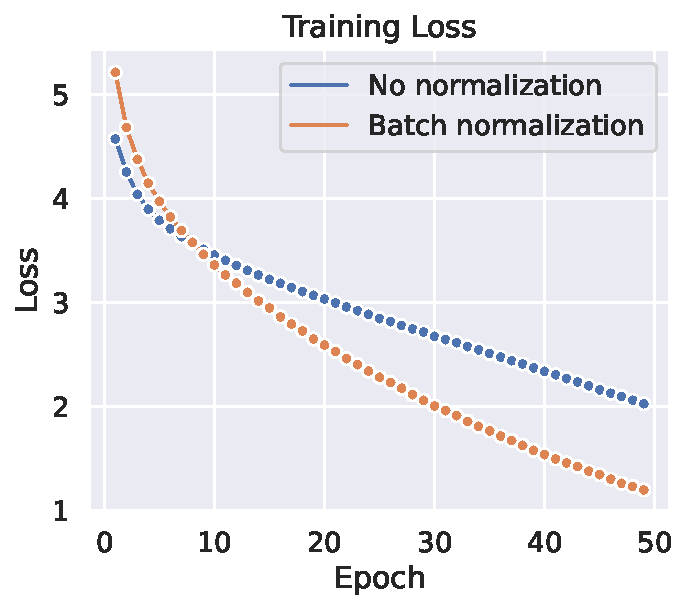
\includegraphics[width=.4\textwidth]{figures/loss_plot.pdf}
% \vspace{-.5cm}
% \caption{Training loss of MLP with (orange) and without (blue) batch normalization on the CIFAR100 dataset.}
% \label{MF:fig:training_loss}
% \end{figure}

\section{Limitations and Future Directions}
In this chapter, we presented a theoretical framework that bridges the gap between the mean field theory of neural networks with finite and infinite widths, with a focus on batch normalization at initialization. Many questions that were out of the scope for this study, suggesting directions for new lines of inquiry. 


\paragraph{Rapidly mixing assumption.}
One limitation of our work is the rapidly mixing assumption that was used to establish the concentration of our results. While our experiments validated our results based on this assumption, it would be beneficial to prove that this assumption holds for a wide range of neural networks with batch normalization.

\paragraph{Training and optimization.}
While our focus of the current work was on random neural networks. In an elegant observation, ~\citet{feng2022rank} demonstrate that the rank of input-output Jacobian of neural networks without normalization at initialization diminishes at an exponential rate with depth (Theorem 5), which implies changes in the input does not change the direction of outputs. In a remarkable observation, ~\citet{yang2018a} show the exact opposite for BN-MLP using a mean field analysis (Theorem 3.10): any slight changes in the input lead to unbounded changes in the output. These results naturally raise the following question: Can we arrive at non-trivial results about input-output Jacobian at the infinite depth finite width regime? 

The mean field approach is also used to analyze the training mechanism. In particular,~\citet{bach2021gradient} prove that gradient descent globally converges when optimizing single-layer neural networks in the limit of an infinite number of neurons. Although the global convergence does not hold for standard neural networks, insights from this mean field analysis can be leveraged in understanding the training mechanism.  

\paragraph{Exploring other normalizations.}
More research is needed for other normalization techniques, such as weight normalization~\cite{salimans2016weight} or layer normalization~\cite{ba2016layer} to understand the impact of these normalization techniques on the robustness and generalization of neural networks. Our findings highlight the power of mean field theory for analyzing neual networks with normalization layers.

\paragraph{Extending to other architectures}
Our analyses are limited to MLPs. Extending our work to convolutional neural networks and transformers would enable us to analyze and enhance initialization for these neural networks. In particular, recent studies have shown that transformers suffer from the rank collapse issue when they grow in depth~\cite{anagnostidissignal}. A non-asymptotic mean field theory may enable us to tackle this issue by providing a sound understanding of representation dynamics in transformers.

Overall, our results demonstrate that depth is not necessarily a curse for mean field theory, but can even be a blessing when neural networks have batch normalization. The inductive bias provided by batch normalization controls the error propagation of mean field approximations, enabling us to establish non-asymptotic concentration bounds for mean field predictions. This result underlines the power of mean field analyses in understanding the behavior of deep neural networks, thereby motivating the principle development of new initialization and optimization techniques for neural networks based on mean field predictions. 



\chapter{Obtaining isometry with normalization}\label{ch:isometry_normalization}

Normalization layers, such as batch normalization~\citep{ioffe2015batch} and layer normalization~\citep{ba2016layer}, are essential components of neural architecture design. They have been shown to improve the training stability and speed of deep neural networks~\citep{he2016deep, devlin2018bert}. In this chapter, we explore the isometry properties of normalization layers. While in Chapter~\ref{ch:bn_ortho}, we focused on the orthogonality properties of normalization layers, here we investigate the isometry properties of these layers, which will be formalized later. This chapter is dedicated to one of the primary results of this thesis, which is the isometry bias of normalization layers. While conceptually orthogonal and isometry properties are related, the striking property of isometry is that it holds deterministically for all matrices, while orthogonality properties discussed in Chapter~\ref{ch:bn_ortho} hold in expectation, with respect to a particular initialization of the weights. 


\section{Gram matrices and isometry}
Given $n$ data points $\{x_i\}_{i\le n}\in \R^d$, the Gram matrix $G^\ell$ of the feature vectors $x_1^\ell,\dots,x_n^\ell \in\R^d$ at layer $\ell$ of the network is defined as
\begin{align}  \label{iso:eq:gram_matrix}
G^\ell := \left[\ip{x^\ell_i}{x_j^\ell}\right]_{i,j\le n}  , && \ell=1,\dots,L.
\end{align}

Intuitively, an isometric Gram matrix implies that the network preserves the distances and angles between the input data points after mapping them to the feature space. 
Isometry of Gram matrices can be quantified using the eigenvalues of $G^\ell.$  
One possible way to formulate isometry is to use the ratio of the volume and scale of the parallelepiped spanned by the feature vectors $x_1^\ell,  \dots,x^\ell_n$. 
For example, consider two points on a plane $x_1, x_2 \in \mathbb{R}^2$ with lengths $a = |x_1|, b = |x_2|$ and angle $\theta = \angle(x_1, x_2)$. The ratio is given by $a b \sin(\theta) / (a^2 + b^2)$, which is maximized when $a=b$ and $\theta = \pi/2$. This is shown for $n=2$ and $n=3$ feature vectors in Figure~\ref{iso:fig:isometry}. 

\begin{figure}[ht]
    \centering
    \begin{tikzpicture}[scale=.40]

\draw (5,-3) node{$ \frac{\norm{x_1} \norm{x_2}\sin\theta}{\frac12(\norm{x_1}^2+\norm{x_2}^2)}$}
(20,-3) node{$\frac{\text{Vol}(\{x_i\}_{i\le n})^{2/n}}{\frac1n\sum_i^n \norm{x_i}^2} = \frac{\det(X^\top X)^{1/n}}{\frac1n \tr(X^\top X)}$};
    \foreach \i/\l in {0/0, 6.5/1} {
        \foreach \j/\angle in {0/0, 5.5/30} {
            \coordinate (O) at (\i,\j*1.1);
            \draw[dashed] (O) -- ++(0:5-\l) -- ++(90-\angle:3+\l) -- ++(180:5-\l) -- cycle;
            \draw[->] (O) -- ++(0:5-\l) node[midway,below] {$\vec{x_1}$};
            \draw[->] (O) -- ++(90-\angle:3+\l) node[midway,left] {$\vec{x_2}$};
            \draw (O) ++(.5,0) arc (0:90-\angle:0.5) node[midway,above,right] {$\theta$};
        }
    }
    \foreach \i/\l in {0/0, 7/1} {
        \foreach \j/\angle in {0/0, 5.6/30} {
            \coordinate (O) at (14+\i,\j*1.2);
            \draw[dashed] (O) -- ++(0:5-\l) node(A){} -- ++(90-\angle:3+\l) node(B){} -- ++(180:5-\l) node(C){} -- cycle;
            \draw[dashed] (A) -- ++(1,1);
            \draw[dashed] (B) -- ++(1,1);
            \draw[dashed] (C) -- ++(1,1);
            \draw[dashed] ($(O)+(1,1)$) -- ++(0:5-\l) -- ++(90-\angle:3+\l) -- ++(180:5-\l) -- cycle;

            \draw[->] (O) -- ++(0:5-\l) node[midway,below] {$\vec{x_1}$};
            \draw[->] (O) -- ++(90-\angle:3+\l) node[midway,left] {$\vec{x_2}$};
            \draw[->] (O) -- ++(1,1) node[below] {$\vec{x_3}$};
            % \draw (O) ++(.5,0) arc (0:90-\angle:0.5) node[midway,above,right] {$\theta$};
        }
    }
\end{tikzpicture}
    \caption{A geometric interpretation of isometry: higher volume corresponds to higher isometry.}
    \label{iso:fig:isometry}
\end{figure}

Inspired by this intuition, we can define the isometry of the Gram matrix. 

\begin{definition}
Let $M$ be an $n \times n$ positive semi-definite matrix. We define the \emph{isometry $\Iso(M)$} of $M$ as the ratio of its normalized determinant to its normalized trace:
\begin{align}\label{iso:eq:isometry}
\Iso(M) := \frac{\det(M)^{1/n}}{\frac1n\tr(M)}.
\end{align}
\end{definition}
The function $\Iso(M)$ defined in \eqref{iso:eq:isometry} quantifies how well $M$ approximates the identity matrix $I_n$. We can easily check that $\Iso(M)$ has some desirable properties (see Lemma~\ref{iso:lem:isometry_basic} for formal statements and proofs):
\begin{itemize}
    \item Scale-invariance: Multiplying $M$ by a constant does not affect $\Iso(M)$.%: $\Iso(c M) = \Iso(M)$
    \item Isometry-preserving: $\Iso(M)$ ranges between $0$ and $1$, with $0$ and $1$ corresponding to degenerate and identity matrices respectively.
    \item Isometry gap: $\ID(M)$ lies between $0$ and $\infty,$ with $0$ and $\infty$ indicating identity and degenerate matrices respectively.
\end{itemize}
These properties suggest that $\Iso(M)$ is a suitable function for measuring how close a matrix is to being an isometry, i.e., a transformation that preserves distances between metric spaces. Moreover, there is a clear link between isometry and normalization, which we will explore in the next section. We will often measure how far a matrix is from isometry by its negative log $\ID(M),$ which we will call \emph{isometry gap}.

\paragraph{Basic properties of isometry}
It is straightforward to check isometry obeys the following basic isometry-preserving properties: 
\begin{lemma}\label{iso:lem:isometry_basic}
For PSD matrix $M,$ the isometry defined in~\eqref{iso:eq:isometry} obeys the following properties: 1) scale-invariance $\Iso(c M) = \Iso(M),$ 2) only takes value in the unit range $\Iso(M)\in [0,1]$ 3) it takes its maximum value if and only if $M$ is identity $\Iso(M)=1\iff M=I_n,$ and 3) takes minimum value if and only if $M$ is degenerate $\Iso(M)=0. $
\end{lemma}
\begin{proof}[Proof of Lemma~\ref{iso:lem:isometry_basic}]
 The scale-invariance is trivially true as scaling $M$ by any constant will scale $\det(M)^{1/n}$ and $\tr(M)$ by the same amount. The proof of other properties is a straightforward consequence of writing the isometry in terms of the eigenvalues $\Iso(M) = (\prod_i \lambda_i)^{1/n}/(\frac1n\sum_i \lambda_i ), $ where $\lambda_i$'s are eigenvalues of $M.$ By arithmetic vs geometric mean inequality over the eigenvalues we have $(\prod_i \lambda_i)^{1/n}\le \frac1n\sum_i \lambda_i ),$ which proves that $\Iso(M)\in [0,1].$ Furthermore, the inequality is tight if and only if the values are all equal $\lambda_1 = \dots =\lambda_n,$ which holds only for an identity $M=I_n$. Finally, the isometry is zero if and only if at least one eigenvalue is zero, which is the case for degenerate matrix $M.$ 
\end{proof}


\section{Isometry bias of normalization}

This notion of isometry has a remarkable property: if we normalize each point by its Euclidean norm  then the isometry of their associated Gram matrix does not decrease. We formalize this property in the following theorem.


\begin{theorem}\label{iso:thm:isometry_normalization}
Given $n$ samples $\{x_i\}_{i\le n}\subset \R^d\setminus\{\0_d\}$, and their projection onto the unit sphere $\Norm{x}_i:=x_i/\norm{x_i},$ and their respective Gram matrices $G = \left[\ip{x_i}{x_j}\right]_{i,j\le n}$ and $\Norm{G} = \left[\ip{\Norm{x_i}}{\Norm{x_j}}\right]_{i,j\le n}.$ The isometry of Gram matrices obeys
\begin{align}
 \Iso\left(\Norm{G}\right) \ge \Iso(G)\left(1+\frac{\frac1n \sum_i^n(a_i-\bar{a})^2}{\bar{a}^2}\right), && \text{where } a_i:=\norm{x_i}, \bar{a}:=\frac1n\sum_i^n a_i. 
\end{align}
\end{theorem}

Theorem~\ref{iso:thm:isometry_normalization} shows a subtle property of normalization: Because the terms $(a_i-\Bar{a})^2$ are always non-negative, the left-hand side is always greater than or equal to $\Iso(G).$ It further quantifies the improvement in isometry as a function of variation of norms. The terms $\Bar{a}$ and $\frac1n \sum_i^n(a_i-\bar{a})^2$ correspond to the sample mean and variance of $a_1,\dots,a_n.$ 
Thus, the more diverse the norms, the larger the improvement in isometry. 
% Note the isometry does not increase if and only if the norms are all equal $a_1=\dots=a_n.$

% \section{Proof of Theorem~\ref{iso:thm:isometry_normalization} and properties of isometry}\label{iso:sec:isometry_theorems}


% \subsection{Proof of Thm~\ref{iso:thm:isometry_normalization} }

\begin{proof}[\textbf{Proof of Theorem~\ref{iso:thm:isometry_normalization}}] 
Define $D :=\diag(a_1/\sqrt{d} ,\dots, a_n/\sqrt{d}).$ Observe that $C = D \Norm{G} D,$ implying $ \det(G) = \det(\Norm{G}) \det(D)^{2}.$ Because $\Norm{x_i}$'s have norm $\sqrt{d},$ diagonals of  Gram after normalization are constant $\Norm{G}_{ii}=d,$ implying $\frac1n\tr(\Norm{G})= d.$ We have
\begin{align}
\frac{\Iso(\Norm{G})}{\Iso(G)}
&=
\frac{\frac1n\tr(G)}{\frac1n\tr(\Norm{G})}\frac{\det(\Norm{G})^{1/n}}{\det(G)^{1/n}}\\
&= \frac{\frac1n\sum_i^n a_i^2}{d}\frac{\det(\Norm{G})^{1/n}}{\det(\Norm{G})^{1/n}(d^{-n} \prod_i^n a_i^2)^{1/n}}\\
&= \frac{(\frac1n\sum_i a_i)^2}{(\prod_i^n a_i)^{2/n}}\frac{\frac1d\sum_i^n a_i^2}{(\frac1n\sum_i a_i)^2}\\
% & \geq  \frac{\frac1n\sum_i^n a_i^2}{(\frac1n\sum_i^n a_i)^2}\\
&= 1+\frac{\frac1n \sum_i^n(a_i-\bar{a})^2}{\bar{a}^2}, && \bar{a}:=\frac1n\sum_i^n a_i
\end{align}
\end{proof}




\section{Implications for normalization layers}
Theorem~\ref{iso:thm:isometry_normalization} allows us to highlight the isometry bias of layer and batch normalization. 


\begin{corollary} \label{iso:cor:ln}
Consider $n$ vectors before and after layer-normalization $\{x_i\}_{i\le n}\subset \R^d\setminus\{\0_d\}$ and $\{\Norm{x}_i\}_{i\le n}, \Norm{x_i}:=\ln{x_i}.$
Define their respective Gram matrices $G := [\ip{x_i}{x_j}]_{i,j\le n},$ and $\Norm{G}:=[\ip{\Norm{x}_i}{\Norm{x}_j}]_{i,j\le n}.$ We have:
\begin{align*}
 \Iso\left(\Norm{G}\right) \ge \Iso(G)\left(1+\frac{\frac1n \sum_i^n(a_i-\bar{a})^2}{\bar{a}^2}\right), && \text{where } a_i:=\norm{x_i},\bar{a}:=\frac1n\sum_i^n a_i. 
\end{align*}
% with equality holding if and only if columns have equal norms $a_1=\dots=a_n$.
\end{corollary}

Observe that we can view the layer normalization as a projection onto the $\sqrt{d}$-sphere, which is equivalent to the unit-norm projection in Theorem~\ref{iso:thm:isometry_normalization} up to a constant scale factor. Since isometry is scale-invariant, this implies that corollary~\ref{iso:cor:ln} follows directly from Theorem~\ref{iso:thm:isometry_normalization}. 

Moreover, corollary~\ref{iso:cor:ln} shows that the isometry of layer normalization is deterministic and does not rely on random weights. This means that layer normalization always preserves or enhances the isometry of representations, even during training. We provide empirical evidence for this in discussion.

Despite the seemingly vast differences between layer normalization and batch normalization, the following corollary shows an intimate link between them through the prism of isometry. 

\begin{corollary} \label{iso:cor:bn}
 Given $n$ samples in a mini-batch before $X\in\R^{d\times n},$ and after normalization $\Norm{X}=\BN{X}$
 and define covariance matrices $C := X X^\top $ and $\Norm{C}:=X X^\top. $ We have:
\begin{align*}
 \Iso\left(\Norm{C}\right) \ge \Iso(C)\left(1+\frac{\frac1d \sum_i^d(a_i-\bar{a})^2}{\bar{a}^2}\right), && \text{where } a_i:=\norm{X_{i\cdot}},\bar{a}:=\frac1n\sum_{i=1}^d a_i. 
\end{align*}
\end{corollary}

Gram matrices of networks with batch normalization have been the subject of many previous studies at network initialization: it has been postulated that BN prevents rank collapse issue~\citep{daneshmand2020batch} and that it orthogonalizes the representations~\citep{daneshmand2021batch}, and that it imposes isometry~\citep{yang2018a}. The isometry results implied by Corollaries~\ref{iso:cor:bn} give a geometric interpretation of all these findings: it is straightforward to verify that maximum isometry is achieved with identity Gram matrix, which implies orthogonalization of these results. Rather strikingly, while all the results stated before have been of a probabilistic nature, the improved isometry of the Gram matrix implied by Corollary~\ref{iso:cor:bn} holds deterministically.

% !TEX root = ../thesis-index.tex

\chapter{Fixed-points and global convergence of deep representations}
\label{ch:isometry_activation}

The study of neural networks has increasingly focused on understanding the internal mechanisms that govern their learning and generalization capabilities. A central aspect of this inquiry is how neural networks transform and preserve input data structure as it passes through multiple layers. One powerful approach to studying these transformations is through the lens of kernel methods, which have long been used in machine learning to understand the relationships between data points in high-dimensional spaces~\cite{scholkopf2002learning,smola2004tutorial}.

Studying neural networks from the perspective of kernels has been the subject of many theoretical studies. This perspective has led to significant advancements, such as the development of Neural Tangent Kernels (NTKs)~\cite{jacot2018neural} and Convolutional Kernel Networks~\cite{mairal2014convolutional}, or in the notion of dual kernel~\cite{daniely2016toward}. The idea that neural networks, especially in the infinite-width limit, can be understood through kernels has been explored in various recent works~\cite{lee2019wide, arora2019exact, yang2019scaling}. Moreover, the use of kernel methods to measure the similarity between inputs as the network processes them provides a powerful means of understanding the inductive biases and representative capacity of neural networks, particularly in the context of deep learning~\cite{zhang2017understanding,zhang2021understanding,cho2009kernel}.

However, the question of how the inner product between hidden layer representations evolves across layers and whether it converges globally to a fixed point remains an important but underexplored area of study~\cite{saxe2013exact, schoenholz2016deep, pennington2018emergence}. While previous research has provided insights into local behaviors~\cite{yang2018a}, a global analysis of fixed points and convergence properties of kernel sequences, particularly in the presence of nonlinear activations, still needs to be improved.

This chapter addresses this gap by introducing and analyzing the evolution of the kernel through layers. The kernel sequence tracks the similarity between two inputs. More concretely, we consider the kernel sequence $k(h^\ell(x), h^\ell(y)),$ where $k$ denotes some notion of similarity, such as inner product or cosine similarity, and $h^\ell(x)$ and $h^\ell(y)$ denote layer $\ell$ representation for respective inputs $x$ and $y$. Understanding whether and how this sequence converges to a fixed point as the network depth increases is crucial for uncovering the inherent implicit biases of deep networks.

Our analysis builds upon foundational work in understanding the role of activation functions in neural networks, such as the use of ReLU and its variants~\cite{glorot2011deep, nair2010rectified} and the exploration of nonlinear activations in large-scale models~\cite{ramachandran2017searching, clevert2015fast}. Additionally, the interplay between activation functions and normalization techniques, such as layer normalization~\cite{ba2016layer}, plays a critical role in shaping the convergence behavior of kernel sequences~\cite{klambauer2017self, hayou2019impact}. Moreover, the study of neural networks through the lens of kernel methods is deeply connected to earlier work on Gaussian processes~\cite{williams2006gaussian} and the dynamics of signal propagation in deep networks~\cite{poole2016exponential, raghu2017expressive}. By analyzing how these kernels evolve across layers, particularly in terms of activation functions, we contribute to a deeper understanding of the dynamics within deep neural networks.

Throughout this chapter, we assume that the network operates under the mean field regime, which simplifies the analysis by tending width to infinity and making stochastic sequences deterministic. 

\section{Preliminaries}
In this section, we introduce the fundamental concepts, notations, and definitions used throughout this chapter. 

We consider a feed-forward neural network with $L$ layers, each with width $d$. The network takes an input vector $x \in \mathbb{R}^d$ and maps it to an output vector $h^L(x) \in \mathbb{R}^d$ through a series of transformations. The hidden representations at each layer $\ell$ are denoted by $h^\ell(x)$. The transformation at each layer is composed of a linear transformation followed by a nonlinear activation function $\phi$. Mathematically, the hidden representation at layer $\ell$ is given by:
\begin{align}
& h^\ell(x) = \phi(W^\ell h^{\ell-1}(x)), && W^\ell \in \mathbb{R}^{d \times d},
\end{align}
where $h^0(x):=x$ is set to input, and elements of $W^\ell$ are drawn i.i.d. from $N(0,1/d)$. The activation function $\phi: \mathbb{R} \to \mathbb{R}$ denotes the activation applied element-wise. 
In some variations of the MLP, we will use normalization layers to adjust the activations at each layer, namely Layer Normalization (LN) or Root Mean Squared (RMS) normalization. Finally, the neural kernel between two inputs $x$ and $y$ at layer $\ell$ is defined as:
\begin{align}
    \rho_\ell = \frac{\langle h^\ell(x), h^\ell(y) \rangle}{\|h^\ell(x)\| \|h^\ell(y)\|},
\end{align}
where $\langle \cdot, \cdot \rangle$ denotes the inner product, and $\rho_0$ corresponds to similiarty between input samples $x$ and $y$.

The main goal of this chapter is to analyze sequence $\{\rho_\ell\},$ at initialization, when the weights are still random. The motivation for this analysis is to understand if various architectural choices, namely activation or number of layers, lead to specific biases of the kernel towards a certain fixed point. Namely, if there is a bias towards zero, it would imply that at initialization, the representations become more orthogonal. In contrast, a positive fixed point would mean the representations become more similar.

In the current setup, the sequence $\{\rho_\ell\}$ is a stochastic sequence or a Markov chain due to the random weights at each layer. 
However, we will show that under the mean field regime, the sequence $\{\rho_\ell\}$ converges to a deterministic sequence, and we will analyze the properties of this deterministic sequence.


\section{Mean field regime}

In this section, we conduct a mean field analysis of multilayer perceptrons (MLPs) to explore the neural kernel's fixed-point behavior as the network depth increases. This approach allows us to gain insight into the global dynamics of neural networks, mainly how the similarity between two input samples evolves as they pass through successive network layers.
Now, we can state the mean field regime for the kernel sequence, stating that in this regime, the sequence becomes deterministic.

\begin{proposition}
\label{iso:prop:mean_field_kernel}
Under the mean field regime, i.e., $d \to \infty$, the kernel sequence $\rho_\ell$ of an MLP with activation $\phi$ that obeys $\E_{X\sim N(0,1)} \phi(X)^2=1.$ Then the sequence evolves deterministically as follows:
\begin{align*}
&\rho_{\ell} = \mathbb{E}_{X,Y}[\phi(X)\phi(Y)], && 
\text{where } X, Y\sim N(0,1),\; \E XY = \rho_{\ell-1}.
\end{align*}
where the initial value $\rho_0$ corresponds to the input. 

\end{proposition}

Historically, conditions similar to $\E \phi(X)^2=1$ have been used to prevent the forward pass from vanishing or exploding. For example, applying ReLU will zero out half of the activations, which will lead to a vanishing norm of forward representations, and Kaiming He's initialization~\citet{he2016deep} addresses that by scaling weights to maintain consistent forward pass norms across layers. This principle is further refined in a self-normalizing activation~\citet{klambauer2017self}, ensuring consistent mean and variances between pre- and post-activations. 


\begin{proof}
 The proof is a straightforward application of the law of large numbers, as the mean field regime implies that the sample means converge to the population means. Let us inductively assume that at layer $\ell$ the it holds that $\frac1d\|h^{\ell}(x)\|^2 = 1$ and $\frac1d\|h^{\ell}(y)\|^2=1,$ and $\frac1d\langle h^{\ell}(x),h^{\ell}(y)\rangle = \rho_{\ell}$. Thus, if $X$ and $Y$ denote the pre-activations for a given unit for the two inputs at layer $\ell$, they follow standard Gaussian distribution and have covariance $\rho_{\ell}.$ By construction we have $\E \phi(X)^2 = \E \phi(Y)^2 = 1$, and $\E \phi(X)\phi(Y) = \rho_{\ell+1}.$ Finally, since each hidden unit is independent of others, based on the law of large numbers, we can conclude the samples means will converge to their expectation $\frac1d \|h^{\ell+1}(x)\|^2 = 1, $ $\frac1d \|h^{\ell+1}(y)\|^2 = 1,$ and $\frac1d \langle h^{\ell+1}(x),h^{\ell+1}(y)\rangle = \rho_{\ell+1}. $ This concludes the proof. 
\end{proof}

As you can see, this proposition shows that the kernel sequence $\rho_\ell$ converges to a deterministic sequence. We can relax the conditions on the weights to allow any distribution with zero mean and variance $1/d,$ such as uniform distribution. 

\begin{proposition}
\label{iso:prop:mean_field_kernel_general}
Under the mean field regime, i.e., $d \to \infty$, the kernel sequence $\rho_\ell$ of an MLP with activation $\phi$ that obeys $\E \phi(X)^2=1.$ If each element of the weights is drawn i.i.d. from a distribution with zero mean and $1/d$ variance, then the sequence evolves deterministically as given by Proposition~\ref{iso:prop:mean_field_kernel}.
\end{proposition}

\begin{proof}
 The key observation is that the pre-activations to each unit can be written as the sum of i.i.d. elements; by Central Limit Theorem, we can conclude that as $d\to\infty,$ their distribution converges to a normal distribution, which allows us to apply Proposition~\ref{iso:prop:mean_field_kernel}.
\end{proof}




Propositions \ref{iso:prop:mean_field_kernel} and \ref{iso:prop:mean_field_kernel_general} under the condition that under some normality conditions on activations,  showed the sequence evolution is entirely determined by a single parameter $\rho_{\ell-1}$, which evolves deterministically, 
Inspired by this property, we define it as the mapping between the covariance of pre-activations and the covariance of post-activations.

\begin{definition}
    \label{iso:def:kernel_map}
Given two random variables $X, Y$ with covariance $\rho,$ and activation $\phi,$ define the \emph{kernel map } $\kappa$ as the mapping between the covariance of pre-activations and the covariance of post-activations:
\begin{align}\label{iso:eq:kernel_map}
    \kappa(\rho):=\E_{X,Y}[ \phi(X)\phi(Y)], && \text{where } X, Y\sim N(0,1),\; \rho:=\E XY.
\end{align}
\end{definition}

With this definition, we can express the result of Propositions~\ref{iso:prop:mean_field_kernel} and~\ref{iso:prop:mean_field_kernel_general} in terms of the kernel map. Under the same setting as Proposition~\ref{iso:prop:mean_field_kernel_general}, the kernel sequence $\{\rho_\ell\}$ evolves deterministically according to the kernel map $\kappa$:
\begin{align}
    \rho_{\ell} = \kappa(\rho_{\ell-1}),
\end{align}
where $\kappa$ is defined in Definition~\ref{iso:def:kernel_map}.  Thus, in order to understand the convergence of sequence $\{\rho_\ell\},$ we can study the fixed-points of the kernel map $\kappa,$
which are the values of $\rho^*$ that satisfy $\kappa(\rho^*) = \rho^*.$ With the assumptoin that $\E \phi(X)^2=1,$ the kernel map $\kappa$ is a mapping between $[-1,-1]$ to itself. Thus, Brower's fixed-point theorem implies that the kernel map $\kappa$ has at least one fixed point $\rho^*.$ But as we will show, there is potentially more than one fixed point, and it will be interesting to understand which ones are locally or globally attractive. 


\section{Hermite expansion of activation functions}
Hermite polynomials possess completeness and orthogonality under the Gaussian weight kernel. This means that any function in the space of square-integrable functions with respect to the Gaussian kernel can be expressed as a linear combination of Hermite polynomials. The square integrability of an activation function ensures that it does not lead to exploding activations, as non-square integrable functions suggest heavy-tailed post-activations that lack second moments, and it holds for all activations that are used in practice. We use the \emph{normalized} Hermite polynomials and their coefficients. 

\begin{definition}
Define normalized Hermite polynomials $\he_k(x)$ as a scaled version of the probabilist's Hermite polynomials $\He_k(x)$, as follows
\begin{align*}
&\He_k(x) :=(-1)^k e^{x^2/2} \frac{d^k}{dx^k} e^{-x^2/2}, && \he_k(x):=\frac{1}{\sqrt{k!}} \he_k(x).
\end{align*}
\end{definition}

Here is a list of the first few normalized Hermite polynomials:

\begin{table}[ht]
    \centering
    \caption{Hermite polynomials and their normalized versions}
    \begin{tabular}{|c|c|c|c|c|c|}
    \hline
 Order & $k=0$ & $k=1$ & $k=2$ & $k=3$ & $k=4$ \\
 \hline
 $\He_k(x)$ & $1$ & $x$ & $ (x^2 - 1)$ & $(x^3 - 3x)$ & $(x^4 - 6x^2 + 3)$ \\    
 \hline
 $\he_k(x)$ & $1$ & $x$ & $\frac{1}{\sqrt{2}} (x^2 - 1)$ & $\frac{1}{\sqrt{6}} (x^3 - 3x)$ & $\frac{1}{\sqrt{24}} (x^4 - 6x^2 + 3)$ \\
    \hline
    \end{tabular}
\end{table}

Most importantly, Hermite polynomials satisfy the orthogonality property:
\begin{align}\label{iso:eq:hermite_orthogonality}
    &\E_{x\sim N(0,1)} \left[\He_k(x)\He_l(x)\right] = k! \delta_{kl}, &&\E_{x\sim N(0,1)} \left[\he_k(x)\he_l(x)\right] = \delta_{kl},
\end{align}
where $\delta_{kl}$ is the Dirac delta. Here we can see the motivation behind our normalization, as it cancels out with the factorial term in the orthogonality property. 

Based on this property, we can express any function $\phi$ as a linear combination of Hermite polynomials:

\begin{definition}\label{iso:def:hermite_expansion}
Given an activation function $\phi$ that is square-integrable with respect to the Gaussian kernel $\int_{-\infty}^\infty \phi(x)^2 e^{-x^2/2}dx < \infty$, the Hermite expansion of $\phi$ is defined as:
\begin{align*}
\phi(x) = \sum_{k=0}^\infty c_k \he_k(x),&&c_k = \E_{X\sim N(0,1)} \left[\phi(X) \he_k(X)\right],
\end{align*}
where $\he_k(x)$ are the normalized Hermite polynomials and $c_k$ are the Hermite coefficients. 
\end{definition}

% Based on the orthogonality of Hermite polynomials, we can make a few observations about some of the Hermite coefficients.  

Besides orthogonality, Hermite polynomials have another magical property that is crucial for our later analysis. 

\begin{lemma}[Consequence of Mehler's kernel]\label{iso:lem:mehler_kernel}
If $X,Y \sim N(0,1)$ with covariance $\E XY = \rho$ we have 
$$\E_{X,Y} \he_n(X)\he_k(Y) = \rho^n \delta_{nk}$$
where $\delta_{nk}$ is the Dirac delta.  
\end{lemma}

This lemma states that given two Gaussian random variables $X, Y$ with covariance $\rho,$, the expectation of the product of Hermite polynomials is zero unless the indices are equal. 

\begin{proof}[Proof of Lemma~\ref{iso:lem:mehler_kernel}]
The property can be deduced from Mehler's formula~\cite{mehler1866ueber}. The formula states that 
\begin{align*}
&\frac{1}{\sqrt{1-\rho^2}}\exp\left(-\frac{\rho^2(x^2+y^2)-2xy\rho}{2(1-\rho^2)}\right) \\
&= \sum_{m=0}^\infty \he_m(x)\he_m(y),
\end{align*}
where the $m!$ factor difference is due to the definition of Hermite polynomials with an additional $1/\sqrt{m!}$ compared to the one used in Mehler's kernel. 
Observe that the left-hand side is equal to $p(x,y)/p(x)p(y)$, where $p(x,y)$ is the joint PDF of $(X, Y)$, and $p(x),p(y)$ are PDF of $X$ and $Y$ respectively. Therefore, we can take the expectation using the expansion 
\begin{align*}
\E_{X,Y}\left[ \he_n(X) \he_k(Y)\right] &= \int \he_n(x)\he_k(y)p(x,y)dx dy \\
&=  \sum_{m=0}^\infty \rho^m\int \he_n(x)\he_k(y) \he_m(x)\he_m(y) dp(x)dp(y)\\
&= \sum_{m=0}^\infty \rho^m\E_{X\sim N(0,1)} \left[\he_n(X)\he_m(X)\right]\E_{Y\sim N(0,1)} \left[\he_k(Y)\he_m(Y)\right] \\
&= \rho^n \delta_{nk} 
\end{align*}
where in the last line we used the orthogonality property $\E_{X\sim N(0,1)} H_k(x) H_n(X)=\delta_{nk}$. 
\end{proof}

Lemma~\ref{iso:lem:mehler_kernel} is crucial for our theory. Based on this lemma, we can express the kernel map in terms of the Hermite coefficients, showing a particular structure of the kernel map.

\begin{corollary}
    \label{iso:cor:hermite_covariance}
    \label{iso:cor:kernel_map}
Given $X,Y \sim N(0,1)$ with covariance $\E X Y = \rho,$ and $\phi(X) = \sum_{k=0}^\infty c_k \he_k(X),$ we have
\begin{align*}
\kappa(\rho) = \E_{X\sim N(0,1)} \left[\phi(X)\phi(X)\right] = \sum_{k=0}^\infty c_k^2 \rho^k.
\end{align*}
\end{corollary}

\begin{proof}[Proof of Corollary~\ref{iso:cor:hermite_covariance}]
Using Lemma~\ref{iso:lem:mehler_kernel} we have
\begin{align*}
\E_{X\sim N(0,1)} \left[\phi(X)\phi(X)\right] = \E_{X\sim N(0,1)} \left[\sum_{k=0}^\infty c_k \he_k(X)\sum_{l=0}^\infty c_l \he_l(X)\right] = \sum_{k=0}^\infty c_k^2 \rho^k.
\end{align*}
\end{proof}

These algebraic properteis of kernel map will be crucial in our analysis of the convergence of the kernel sequence to a fixed point. Before we turn our attention to convergence, let us draw some links between the properties of activation functions, its kernel map, and its Hermite coefficients.

\begin{table}[ht]
    \centering
    \caption{Properties of activations in terms of Hermite coefficients and kernel map}
    \begin{tabular}{|c|c|c|c|}
    \hline
 Property & Activation $\phi$ & Hermite coefficients $\{c_k\}_{k\ge 0}$ & Kernel map $\kappa$ \\
    \hline
 Centered & $\E \phi(X)=0$ & $c_0 = 0$ & $\kappa(0) = 0$ \\
    \hline
 Stable & $\E \phi(X)^2 = 1$ & $\sum_{k=0}^\infty c_k^2 = 1$ & $\kappa(1) = 1$ \\
    \hline
 Non-linear & $\phi(x)$ is non-linear & $\sum_{k=2}^\infty c_k^2 > 0$ & $\kappa(\rho)$ is non-linear \\
    \hline
    \end{tabular}
\end{table}


\section{Globally contracting kernel to zero}

Recall that for activations that obey $\E \phi(X)^2 = 1,$, the kernel map  $\kappa$ is a power series with non-negative coefficients $\sum_k c_k \rho^k$ that maps $[-1,1]$ to itself, and obeys $\kappa(1)=1.$ This immediately reveals that $\rho=1$ is a fixed point of the kernel map. This is unsurprising, as it reaffirms the fact that if two inputs are identical with unit variance, the post-activations will also be identical. However, it is far more interesting whether this fixed point is globally attractive and how the kernel map influences the convergence rate to this fixed point. In a similar vein, we can ask if there are other fixed points and how the kernel map influences the convergence rate to these fixed points.

In the same vein as previous chapters, we are primarily interested in seeing which properties in the kernel maps lead to convergence towards orthogonality. In other words, we are primarily interested in conditions that lead to $\rho^*=0$ being a fixed point and under which conditions this fixed point is globally attractive. 



% A quantity that will be crucial for our analysis is the contraction rate of the kernel map, which is defined based on the Hermite coefficients of the activation function.

% \begin{definition}
%     \label{iso:def:contraction_rate}
%  Given activation $\phi$ that with Hermite coefficients $\{c_k\}_{k\ge 0},$ it contraction rate $\alpha$ is defined as:
%     \begin{align}\label{iso:eq:contraction_rate}
%         \alpha = \frac{\sum_{k=1}^\infty c_k^2}{\sum_{k=1}^\infty  k c_k^2 } = \frac{\kappa(1)-\kappa(0)}{\kappa'(1)}.
%     \end{align}
% \end{definition}

% We can make the following important observation about the range and extreme values of the contraction rate $\alpha.$

% \begin{remark}
%     \label{iso:rem:contraction_rate}
%  Note that the term 
%     $(\sum_{k=1}^\infty c_k^2)/(\sum_{k=1}^\infty k c_k^2)$
%  is always in the range $[0,1].$ Furthermore, $\alpha < 1$ if and only if the activation is non-linear, i.e., $c_k \neq 0$ for some $k\ge 2.$ We can also observe this from the second formulation: the numerator $(\kappa(1)-\kappa(0))/(1-0)$ encodes the slope of the line connecting $(0,\kappa(0))$ and $(1,\kappa(1)),$ and the denominator $\kappa'(1)$ is the slope of the tangent line at $\rho=1.$ Because $\kappa$ is convex in $[0,1]$ the tangent slope is higher than the line slope, which implies $\alpha\le 1,$ and it becomes strict if and only if the convexity is strict, i.e., the activation is non-linear. 
% \end{remark}


Finally, we can state one of the central results of this chapter, which characterizes the global convergence of the kernel map towards the fixed point $\rho^*=0.$

\begin{theorem}\label{iso:thm:global_attract}
Let $\phi$ be an activaiton with kernel map $\kappa$ that is centered $\kappa(0)=0,$ and $\kappa(1)=1.$ Let $\rho_\ell$ be the kernel sequence $\rho_{\ell+1}=\kappa(\rho_\ell),$ given initial value $\rho_0.$ Then, the sequence contracts towards fixed-point zero $\rho^*=0$ with rate $\alpha$:
    \begin{align}
        &\frac{|\rho_\ell|}{1-|\rho_\ell|} \le \frac{|\rho_0|}{1-|\rho_0|}\alpha^{\ell}, && \text{where } \alpha = \frac{1}{2-\kappa'(1)}
    \end{align}
 where $\alpha$ is strictly less than one if the activation is non-linear. The only other fixed points can be $\rho^*=1$ or $\rho^*=-1,$, and none of them is locally or globally attractive.
\end{theorem}

Note that the statement becomes vacuous if the initial covariance is $\rho_0 = 1$ or $\rho_0 = -1$, as in these cases, the right-hand side goes to infinity, but the theorem is non-vacuous for all $\rho_0\in(-1,1).$ This is unsurprising, as the kernel map cannot separate the two inputs if they are identical or anti-identical. In plain words, this states that if the two samples are not identical, by iteratively passing them through a nonlinear activation, the covariance between them will contract with rate $\alpha$ in expectation.  While it may not seem immediately obvious why $\alpha < 1$ for non-linear activations, the following remark makes the connection between the two.

\begin{remark}
    \label{iso:rem:contraction_rate}
    Let us assume $\kappa(\rho)=\sum_{k=0}^\infty c_k^2\rho^k,$ where $c_k$ denote Hermite coefficients. Note that $\kappa'(0) = c_1^2 \le \sum_{k=0}^\infty c_k^2 = \kappa(1)=1$. Now, if we have $\kappa'(1)=1,$ it implies that $c_k=0$ for all $k\ge 2.$ This is a contradiction with the assumption that the activation is non-linear.  
\end{remark}


Another observation is that rather than proving convergence directly, we showed contraction under the potential $|\rho|/(1-|\rho|).$ Because $|\rho|/(1-|\rho|)$ is a monotonically increasing with $|\rho|$, the contraction of $|\rho_\ell|/(1-|\rho_\ell|)$ implies contraction of $|\rho_\ell|$ towards zero. We can state the contraction directly in terms of the sequence $\rho_\ell $.

\begin{corollary}
Under the same setting as in Theorem~\ref{iso:thm:global_attract}, the sequence $\rho_\ell = \kappa(\rho_{\ell-1})$ converges to zero with rate $|\rho_\ell| \le \rho_0/(1-|\rho_0|) \alpha^{\ell}$.
\end{corollary}

The proof follows directly from Theorem~\ref{iso:thm:global_attract} and the inequality $|\rho_\ell| \le |\rho_\ell|\le (1-|\rho_\ell|).$ 


% We can now state and prove the main theorem of this section, which characterizes the global convergence of the kernel map towards the fixed point $\rho^*=0.$

% \begin{theorem}\label{iso:thm:global_attract}
%  Consider activation $\phi,$ that with Gaussian pre-activations, has zero mean $\E_{X}\phi(X)=0$ and unit variance $\E_{X}\phi(X)^2 = 1,$ the sequence $\rho_\ell = \kappa(\rho_{\ell-1})$ contracts towards zero with rate $\alpha$:
%     \begin{align}
%         \Psi(\rho_\ell)\le \Psi(\rho_0) \alpha^{\ell}, 
%     \end{align}
%  where $\alpha$ is defined in \eqref{iso:eq:contraction_rate}, which becomes strictly less than one if the activation is non-linear. 
% \end{theorem}

\textit{Proof idea:} The main proof idea of this theorem is to show that upon applying the kernel map $\kappa$ to the covariance of pre-activations, the potential function $|\rho|/(1-|\rho|)$ decreases with rate $\alpha,$ and applying an induction over $\ell.$ Condition $\kappa(1)=\E \phi(X)^2 = 1$ ensures that activations are stable and do not explode or vanish, allowing us to apply the single step contraction inductively. The proof of the single step follows from the properties of Hermite polynomials and the orthogonality of the kernel map. The non-linearity condition is essential to have $\alpha<1,$ which rules out identity-like activations that do not change the value. The centered condition $\kappa(0)=\E \phi(X) = 0$ ensures that $\rho^*$ is a fixed point.

Some activations, such as SeLU~\citet{klambauer2017self}, which is a self-normalizing activation function that has $\E \phi(X)^1 = 0.$ 

% \begin{proof}
% The proof follows directly from Proposition~\ref{iso:prop:isometry_bias}, by applying induction over $\ell.$
% \end{proof}


\begin{proof}[Proof of Theorem~\ref{iso:thm:global_attract}]
 The main technical part of the proof is to prove that:
    \begin{align*}
        \Psi(\kappa(\rho)) \le \alpha \Psi(\rho), && \Psi(\rho) = \frac{|\rho|}{1-|\rho|}.
    \end{align*}
Base don the given assumptions we have $c_0^2 = \kappa(0) = 0$ and based on the assumption $\E \phi^2(X)=1$ and properties of Hermite polynomials we have $\kappa(1)=\sum_{k=1}^\infty c_k^2 = 1.$ 
    
 First, we will consider positive $\rho\in[0,1),$ for which we have
    \begin{align*}
 \frac{\Psi(\kappa(\rho))}{\Psi(\rho)}&=\left(\frac{\kappa(\rho)}{1-\kappa(\rho)}\right)  \left(\frac{\rho}{1-\rho}\right)^{-1}\\  
        &= \frac{\rho^{-1}\sum_{k=1}^\infty c_k^2 \rho^{k} }{(1-\rho)^{-1}\sum_{k=1}^\infty c_k^2 (1-\rho^{k})} \\
        &= \frac{\sum_{k=1}^\infty c_k^2 \rho^{k-1}}{\sum_{k=1}^\infty c_k^2 \left(\frac{1-\rho^{k}}{1-\rho}\right)}\\
        &= \frac{\sum_{k=1}^\infty c_k^2 \rho^{k-1}}{\sum_{k=1}^\infty c_k^2 \left(\sum_{i=0}^{k-1}\rho^{i}\right)}\\
        &\le \frac{\sum_{k=1}^\infty c_k^2\rho^{k-1} }{\sum_{k=1}^\infty c_k^2 \rho^{k-1} + \sum_{k=2}^\infty c_k^2}\\
        &\le \max_{\rho\in[0,1]} \frac{\sum_{k=1}^\infty c_k^2\rho^{k-1} }{\sum_{k=1}^\infty c_k^2 \rho^{k-1} + \sum_{k=2}^\infty c_k^2}\\
        &= \frac{\sum_{k=1}^\infty c_k^2}{2\sum_{k=1}^\infty c_k^2 -c_1^2 } \\
        &=\frac{1}{2-\kappa'(0)} =: \alpha.
    \end{align*}
 Now, we can use the fact that the norm of the sum of values is bounded by the sum of their norms to argue that
    \begin{align*}
 |\kappa(\rho)|=|\sum_{k=1}^\infty c_k^2 \rho^k | &\le \sum_{k=1}^\infty c_k^2 |\rho|^k 
 = \kappa(|\rho|)
    \end{align*}
 Because $x\mapsto x/(1-x)$ is monotonically increasing for $x\in[0,1]$, for all $\rho\in[-1,1]$ we have 
    \begin{align*}
 \frac{|\kappa(\rho)|}{1-|\kappa(\rho)|}\le \frac{\kappa(|\rho|)}{1-\kappa(|\rho|)} \le \frac{|\rho|}{1-|\rho|}\alpha.
    \end{align*}
Where we invoked the inequality that was proven for $\rho\in[0,1], $ Plugging in the definition of $\Psi$ we have proven that for all $\rho$ we have
\begin{align*}
    \Psi(\kappa(\rho)) \le \alpha \Psi(\rho).
\end{align*}
We can conclude the proof by induction over $\ell.$

\textit{Other fixed-points:}
What remains to show is that the only possible fixed points are $\rho^*=0,1,-1,$, and only $1,-1$ are neither locally or globally attractive.  

First, by contraction result we have so far, for any $\rho \in (-1,1),\rho\neq 0,$ then $|\kappa(\rho)|$ will be strictly smaller than $|\rho|,$ which contradicts with it being a fixed point. That only leaves $\{-1,0,1\}$ as possible fixed points. Now, we will prove that $-1,1$ are not locally attractive fixed points. 

For $\rho^*=1$ to be locally attracting, we must have $|\kappa'(\rho^*)|<1,$ and by construction we have $\kappa'(0)<1,$ However, this implies in some small $\epsilon$ there is $\rho_0\in(0,\epsilon)$ and $\rho_1 \in (1-\epsilon,1),$ such that we have $\kappa(\rho_0) < \rho_0$ and $\kappa(\rho_1) > \rho_1.$ Now, by continuity of $\kappa(\rho)$ there must be a point $\rho_2\in (\rho_0,\rho_1)$ such that $\kappa(\rho_2) = \rho_2,$ which contradicts the assumption that $\rho^*=1$ is the only fixed point. The same argument can be made for $\rho^*=-1.$ 

Thus, we have shown that only $\{-1,0,1\}$ can be fixed-point, and only $\rho^*=0$ is globally attractive.
\end{proof}



\section{Convergence of the kernel with general activations}
So far, we only discussed the convergence of the kernel map for activations that are centered and the convergence of their kernel sequence towards zero. However, we can extend this analysis to general activations that are not centered. In this section, we will show that for any activation function that is non-linear, there is a unique fixed point $\rho^*$ that is globally attractive.


\begin{theorem}
Let $\kappa$ be the kernel map satisfying $\kappa(1)=1$. Define the kernel sequence $\rho_{\ell+1}=\kappa(\rho_\ell)$, with initial step $\rho_0 \in (-1,1)$. Assuming that the activation is non-linear, there is a unique $\rho^*\in[0,1]$ such that $\kappa(\rho^*) = \rho^*$, and $\kappa'(\rho^*) < 1.$ Furthermore, we have the following contraction rate towards $\rho^*$:
\begin{enumerate}
    \item If $\kappa(0)=0$, then $\rho^*=0$ is an attracting with rate 
    \begin{align}
    \frac{|\rho_\ell|}{1-|\rho_\ell|} \le \frac{|\rho_0|}{1-|\rho_0|} (1/\kappa'(1))^\ell
    \end{align}
    \item If $\kappa(0)>0$ and $\kappa'(1)<1$, then $\rho^*=1$ is an attracting, with rate 
    \begin{align}
    |\rho_\ell-1| \le |\rho_0-1| (\kappa'(1))^\ell
    \end{align}
    \item If $\kappa(0) > 0$, and $\kappa'(1)=1$ then  $\rho^*=1$ is attracting with rate 
    \begin{align}
    |\rho_\ell-1| \le \frac{|\rho_0-1|}{\ell\alpha|\rho_0-1|+1}, && \alpha = 1-\kappa(0)-\kappa'(0).
    \end{align}
    \item If $\kappa(0) > 0$, and $\kappa'(1)>1$ then the attracting fixed point is necessarily in the range $\rho^*\in(0,1)$, we have  
    \begin{align}
    &|\rho_\ell-\rho^*| \le \frac{|\rho_0-\rho^*|}{1-|\rho_0|}\alpha^\ell && \alpha = \max\left\{1-\kappa(0),\kappa'(\rho^*),\frac{1-\rho^*}{2-\kappa'(\rho^*)}\right\},
    \end{align}
    where $\alpha$ is strictly less than one if the activation is non-linear.
\end{enumerate}
\end{theorem}

\begin{remark}
The assumptions laid out in the theorem are nearly tight. For example, the non-linearity assumption is necessary to rule out identity activation, where every point in $[-1,1]$ is a fixed point. Furthermore, considering odd activations such as $\phi(x) = x^3,$ and we can see that if $\rho_0\in\{-1,1\}$, the sequence will remain the same $\rho_\ell=\rho_0,$ and hence will not converge, which implies the condition that $\rho_0\in(-1,1)$ is necessary. 
\end{remark}

\begin{remark}
Note that all convergence rates are of exponential form $\|\rho_\ell-\rho^*\|= O(\alpha^\ell),$ where $\alpha<1$ if the activation is non-linear, with the exception of the case where $\kappa'(1)=1,$ where the rate is of the form $O(1/\ell).$ 
\end{remark}

\begin{proof}
We will cases individually, starting with the first case that falls direclty under a previous theorem. 

\subsection*{Case 1: $\kappa(0)=0$}
We can observe that the case where $\kappa(0)=0,$ falls directly under Theorem~\ref{iso:thm:global_attract}, and thus there is no need to prove it again.

\subsection*{Cases 2,3: $\kappa(0)>0$ and $\kappa'(1)\le 1$} In this part, we jointly consider two cases where $\kappa(0)>0$ and $\kappa'(1) < 1,$ and $\kappa'(1)=1.$ Let us consider the ratio between distances $|\rho_\ell-1|$:
\begin{align*}
    \frac{|\kappa(\rho)-1|}{|\rho-1|} &= \frac{1-\kappa(\rho)}{1-\rho} \\
    &=\frac{\kappa(1)-\kappa(\rho)}{1-\rho}\\
    &=\frac{\sum_{k=1}^\infty c_k^2 (1-\rho^k)}{1-\rho}\\
    &=\sum_{k=1}^\infty c_k^2 \sum_{i=0}^{k-1}\rho^i\\
\implies \frac{|\kappa(\rho)-1|}{|\rho-1|} &=\kappa'(1)-\kappa'(1)+\sum_{k=1}^\infty c_k^2 \sum_{i=k}^\infty \rho^i\\
&= \kappa'(1)-\sum_{k=1}^\infty c_k^2 \big(k-\sum_{i=k}^\infty \rho^i\big)\\
\end{align*}
Clearly, the term $k-\sum_{i=k}^\infty \rho^i$ is is always non-negative, implying that if $\kappa'(1)<1$ we have the contraction 
\begin{align*}
    \frac{|\kappa(\rho)-1|}{|\rho-1|} \le \kappa'(1) \implies |\rho_\ell-1| \le |\rho_0-1| \kappa'(1)^\ell.
\end{align*}
Otherwise, if $\kappa'(1)=1,$ we have 
\begin{align*}
    \frac{|\kappa(\rho)-1|}{|\rho-1|} = 1-\sum_{k=1}^\infty c_k^2 \big(k-\sum_{i=0}^{k-1} \rho^i\big).
\end{align*}
Now, observe that the first term for $k=1$ is zero. Furthermore, the sequence $k-\sum_{i=0}^{k-1}\rho^i$ is monotonically increasing in $k$. Thus, the smallest value the weighted sum can achieve is if all of the weights of terms above $k\ge 2$ are concentrated in $k=2,$ which leads to the contraction
\begin{align*}
    \frac{|\kappa(\rho)-1|}{|\rho-1|} \le 1-(1-c_0^2-c_1^2)(2-1-\rho) = 1- (1-c_0^2-c_1^2) (1-\rho).
\end{align*}
Now, define sequence $x_\ell:= 1-\rho_\ell,$ and observe that we have 
\begin{align*}
    x_{\ell+1} \le x_\ell (1-\alpha x_\ell), && \alpha = 1-c_0^2-c_1^2,
\end{align*}
where $\alpha > 0$ if the activation is non-linear. 
We can prove inductively that 
\begin{align*}
x_\ell\le \frac{x_0}{\ell\alpha x_0 + 1}.
\end{align*}
If we plug in the definition of $x_n$ we have proven
\begin{align*}
|\rho_\ell-1| \le \frac{|\rho_0-1|}{\ell \alpha |\rho_0-1| + 1}.
\end{align*}

\subsection*{Case 4: $\kappa(0)>0$ and $\kappa'(1)>1$}
The main strategy is to prove some contraction of $\kappa(\rho)$ towards $\rho^*$, under the kernel map $\kappa$. In other words, we need to show $|\kappa(\rho)-\rho^*|$ is smaller than $|\rho-\rho^*|$ under some potential. First, we assume there is a $\rho^*$ such that $\kappa'(\rho^*)<1,$ and show this contraction, and later prove its existence and uniqeness. 

To prove contraction towards $\rho^*$ when $\kappa'(\rho^*)<1$, we consider three cases: 1) If $\rho > \rho^*$, 2) If $\rho \in [0,\rho^*]$, and 3) If $\rho < 0$. However, the bounds will be of different potential forms and will have to be combined later.  Let $\kappa(\rho) = \sum_{k=0}^\infty c_k^2 \rho^k$ be the kernel map with $\kappa(1)= 1$ with fixed-point $\rho^*$ that satisfies $\kappa'(\rho^*)<1.$

\begin{itemize}
\item \textbf{$\rho\ge \rho^*$.} we will prove:
\begin{align*}
\frac{|\kappa(\rho)-\rho^*|}{1-\kappa(\rho)} \le \frac{|\rho-\rho^*|}{1-\rho} \kappa'(\rho^*)
\end{align*}

We have the series expansion around $\rho^*$: $\kappa(\rho) = \rho^* + \sum_{k=1}^\infty a_k (\rho-\rho^*)^k$. For points $\rho\ge \rho^*$, we will have $\kappa(\rho)\ge \rho^*$, thus we can write

\begin{align*}
\frac{\kappa(\rho)-\rho^*}{1-\kappa(\rho)} &= \frac{\sum_{k=1}^\infty a_k (\rho-\rho^*)^k}{\kappa(1)- \kappa(\rho^*)}\\
&= \frac{\sum_{k=1}^\infty a_k (\rho-\rho^*)^k}{\sum_{k=1}^\infty a_k (1-\rho^*)^k - \sum_{k=1}^\infty a_k (\rho-\rho^*)^k}  \\
&= \frac{(\rho-\rho^*)\sum_{k=1}^\infty a_k (\rho-\rho^*)^{k-1}}{(1-\rho)\sum_{k=1}^\infty a_k (\sum_{i=0}^{k-1}(1-\rho^*)^i(\rho-\rho^*)^{k-1-i})} \\
&= \frac{\rho-\rho^*}{1-\rho}\cdot\frac{\sum_{k=1}^\infty a_k (\rho-\rho^*)^{k-1}}{\sum_{k=1}^\infty a_k (\sum_{i=0}^{k-1}(1-\rho^*)^i(\rho-\rho^*)^{k-1-i})}\\
&\le \frac{\rho-\rho^*}{1-\rho}\frac{\sum_{k=1}^\infty a_k (\rho-\rho^*)^{k-1}}{\sum_{k=2}^\infty a_k (1-\rho^*)^{k-1} + \sum_{k=1}^\infty a_k (\rho-\rho^*)^{k-1}}\\
&\le \max_{\rho\in[\rho^*,1]}\frac{\rho-\rho^*}{1-\rho}\frac{\sum_{k=1}^\infty a_k (\rho-\rho^*)^{k-1}}{\sum_{k=2}^\infty a_k(1-\rho^*)^{k-1} + \sum_{k=1}^\infty a_k (\rho-\rho^*)^{k-1}}\\
&\le \frac{\rho-\rho^*}{1-\rho}\frac{\sum_{k=1}^\infty a_k (1-\rho^*)^{k-1}}{\sum_{k=2}^\infty a_k (1-\rho^*)^{k-1} + \sum_{k=1}^\infty a_k (1-\rho^*)^{k-1}}\\
&=\frac{\rho-\rho^*}{1-\rho}\frac{\kappa(1)-\rho^*}{2\kappa(1)-\kappa'(\rho^*)}\\
&=\frac{\rho-\rho^*}{1-\rho}\frac{1-\rho^*}{2-\kappa'(\rho^*)}
\end{align*}
Thus, we have proven that 
\begin{align*}
\rho \ge \rho^* \implies \frac{|\kappa(\rho)-\rho^*|}{1-\kappa(\rho)} \le \frac{|\rho-\rho^*|}{1-\rho} \frac{1-\rho^*}{2-\kappa'(\rho^*)}
\end{align*}

% Now, because we can view the numerator and denominator as weighted sums, with $a_k$ as weights, and considering that the ratio between $(\rho-\rho^*)^{k-1}$ and $\sum_{i=0}^{k-1}(1-\rho^*)^i(\rho-\rho^*)^{k-1-i}$ is monotonically increasing in $\rho$, we can conclude that the ratio is maximized at $\rho$ is maximum, i.e., $\rho=1$. Thus, we can write
% \begin{align*}
% \rho \ge \rho^* \implies \frac{|\kappa(\rho)-\rho^*|}{1-\kappa(\rho)} \le \frac{|\rho-\rho^*|}{1-\rho} \frac{\sum_{k=1}^\infty a_k (1-\rho^*)^{k-1}}{\sum_{k=1}^\infty k a_k (1-\rho^*)^{k-1}} = \frac{|\rho-\rho^*|}{1-\rho} \frac{1-\rho^*}{\kappa'(1)}
% \end{align*}
% For the last step, we can recognize the quantities numerator quantity as $\kappa(1)-\rho^* = 1-\rho^*,$ while the denominator is $\kappa'(1)$. Thus, we have proven 
% \begin{align*}
% \rho \ge \rho^* \implies \frac{|\kappa(\rho)-\rho^*|}{1-\kappa(\rho)} \le \frac{|\rho-\rho^*|}{1-\rho} \frac{1-\rho^*}{\kappa'(1)}
% \end{align*}

\item \textbf{$0\le \rho \le \rho^*$.}
Consider $\rho \in [0,\rho^*]$. For these $\kappa'(\rho)$ is always monotonically increasing, implying that $\kappa'(\rho)\le \kappa'(\rho^*) < 1$. Thus, $|\kappa(\rho)-\rho^*| \le \kappa'(\rho^*) |\rho - \rho^*|$. This implies that in this range $|\kappa(\rho)-\rho^*|$ will contract with a rate $\kappa'(\rho^*)$:
\begin{align*}
0\le \rho \le \rho^* \implies |\kappa(\rho) - \rho^*| \le \kappa'(\rho^*) |\rho-\rho^*|
\end{align*}

\item \textbf{$-1 \le \rho \le 0$.}
Finally, let us consider $\rho \le 0$. Recall that we have $\kappa(1) = 1$. Thus, we can express $\kappa(\rho)-1$ as product of $(\rho-1)$ with some power series $q(\rho)$:
\begin{align*}
\kappa(\rho) - 1 = (\rho-1)q(\rho), \quad q(\rho) = \sum_{k=0}^\infty b_k \rho^k.
\end{align*}
In fact, we can expand $\kappa(\rho)$ in terms of these new coefficients
\begin{align*}
\kappa(\rho) = 1-b_0 + \sum_{k=0}^\infty (b_k - b_{k+1}) \rho^k
\end{align*}
Due to the non-negativity of coefficients of $\kappa$, we can conclude $1\ge b_0 \ge b_1 \ge ...$. Based on this observation, for $0 < \rho < 1$, we can conclude
$q(-\rho) = b_0 - b_1 \rho + b_2 \rho^2 - ... \le b_0$. Because we can pair each odd and even term $-b_{k}\rho^k + b_{k+1} \rho^{k+1}$ for all odd $k$, and because coefficients $b_k \ge b_{k+1}$ and $\rho^{k} \ge \rho^{k+1}$ for $\rho \in [0,1]$, we can argue $q(-\rho) \le b_0 = 1 - c_0^2$. Now, plugging this value into the kernel map for $0 < \rho < 1$, we have:
\begin{align*}
\kappa(-\rho) &= 1 - (1+\rho)q(-\rho) \\
&\ge 1-(1+\rho)(1-c_0^2)\\
&= 1 - 1 - \rho - c_0^2 (1+\rho)\\
&\implies \kappa(-\rho) + \rho \ge c_0^2 (1+\rho)\\
&\implies -\rho + c_0^2(1+\rho) \le \kappa(-\rho) \le \kappa(\rho)
\end{align*}
Now, if we assume $\kappa(-\rho) \le \rho^*$ then
\begin{align*}
\frac{|\kappa(\rho)-\rho^*|}{|-\rho-\rho^*|}=\frac{\rho^* - \kappa(-\rho)}{\rho^* + \rho} \le \frac{\rho^* + \rho - c_0^2 (1+\rho)}{\rho+\rho^*} = 1- \frac{c_0^2(1+\rho)}{\rho+\rho^*} \le 1-c_0^2
\end{align*}
Now, if we assume $\kappa(-\rho) \ge \rho^*$, knowing that $\kappa(-\rho)\le \kappa(\rho)$, which necessitates $\rho\ge \rho^*$, which implies $\kappa(\rho)\le \rho$. Thus, we have
\begin{align*}
\frac{|\kappa(-\rho)-\rho^*|}{|-\rho-\rho^*|} = \frac{\kappa(-\rho)-\rho^*}{\rho+\rho^*}\le \frac{\kappa(\rho)-\rho^*}{\rho+\rho^*} \le \frac{\rho-\rho^*}{\rho+\rho^*} \le \frac{1-\rho^*}{1+\rho^*} \le 1-\rho^*
\end{align*} 
Combining both cases we have 
\begin{align*}
\rho \le 0 \implies \frac{|\kappa(\rho)-\rho^*|}{|\rho-\rho^*|} \le 1 - \min(c_0^2 , \rho^*) = 1-\min(\kappa(0),\rho^*).
\end{align*}
We can further prove that $\rho^* = \kappa(\rho^*) = k(0) + \text{non-negative terms}$, which implies that $\rho^* \ge k(0)$. Thus, we can conclude that 
\begin{align*}
\rho \le 0 \implies |\kappa(\rho)-\rho^*| \le (1 - k(0))|\rho-\rho^*|
\end{align*}
\end{itemize}

\textbf{Positivity, uniqueness, and existence of a globally attractive fixed-point}
Here, the goal is to prove there is exactly one point $\rho^*\in[0,1]$ such that $\kappa(\rho^*) = \rho^*$ and $\kappa'(\rho^*) < 1.$ We will prove the properties of positivity, uniqueness, and existence separately.

\textit{Positivity:} Let us assume that $\rho^* \le 0.$ is a fixed-point. Then, we can apply the contraction rate proven for Case 3, which shows that $\kappa(\rho^*)\ge \rho^* + k(0) > \rho^*,$ which is a contradiction.


\textit{Uniqueness:} Assume that there are two fixed points $\rho_1$ and $\rho_2$ that satisfy $\kappa'(\rho_1),\kappa'(\rho_2)<1.$ Let us assume wlog that $\rho_1 < \rho_2.$ Then we can invoke the contraction rate proven so far to argue that all points in $(-1,1),$ including  $\rho\in (\rho_1,\rho_2)$ are attracted towards both $\rho_1$ and $\rho_2,$ which is a contradiction. Thus, there can be at most one fixed point.

\textit{Existence of $\rho^*$:} Because $\kappa(1)=1$ the set of all fixed-points is non-empty. Let us assume that $\rho^*$ is the first (smallest) fixed point of $\kappa(\rho^*) = \rho^*,$ which because of the positivity result is necessarily $\rho^*>0.$ If we assume that $\kappa'(\rho^*) > 1,$ then in the small $\epsilon$-neighborhood of it $\rho_1 \in(\rho^*-\epsilon,\rho^*)$ we have $\kappa(\rho_1) < \rho_1.$ Because $\kappa(\rho)$ is continuous, and is above identity line at $\rho=0$ and under identity line $\rho=\rho_1,$ there must be a point $0 < \rho_2 < \rho_1$ where it is at identity $\kappa(\rho_2) = \rho_2,$ which is a contradiction with assumption that $\rho^*$ is the smallest fixed point. Thus, we must have $\kappa'(\rho^*) \le 1.$ If we assume that $\kappa'(\rho^*) = 1,$ then the $\kappa$ must align with the identity line from $\rho^*$ to $1,$ which implies that all higher order terms $c_k,k\ge 2$ must be zero, which in turn implies that $\kappa$ is a linear function. This is a contradiction with the assumption that the activation is non-linear. Thus, we must have $\kappa'(\rho^*) < 1,$ which proves the desired existence. 

\textbf{Combining the cases}
Let us summarize the results so far. We have proven the existence of a unique fixed-point $\rho^*\in[0,1]$ such that $\kappa'(\rho^*)< 1,$ and we have proven contraction rates for each of the three cases.
\begin{align*}
\begin{cases}
\frac{|\kappa(\rho)-\rho^*|}{1-\kappa(\rho)} \le \frac{|\rho-\rho^*|}{1-\rho}\frac{1-\rho^*}{2-\kappa'(\rho^*)} & \text{if } \rho \ge \rho^* \\
|\kappa(\rho)-\rho^*| \le \kappa'(\rho^*)|\rho-\rho^*| & \text{if } 0 \le \rho \le \rho^*\\
|\kappa(\rho)-\rho^*| \le (1 - k(0))|\rho-\rho^*| & \text{if } \rho \le 0 
\end{cases}
\end{align*}

Again, we can consider two cases, if $\kappa'(1)<1$ or $\kappa'(1)>1.$ First, note that $\kappa'(1)=1$ is impossible, as it would imply $\kappa'(1)=\sum_{k=1}^\infty k c_k^2 = \sum_{k=0}c_0^2 ,$ which implies that all $c_k=0,$ which is a contradiction with the assumption that the activation is non-linear.

Let us now define the joint decay rate:
\begin{align*}
\alpha = \max\left\{1 - k(0), \kappa'(\rho^*), \frac{1-\rho^*}{1-\kappa'(\rho^*)}\right\}
\end{align*}
In other words, this is the worst-case rate for any of the above cases. 

Now, let us assume we are starting from initial $\rho_0$ and define $\rho_\ell = \kappa(\rho_{\ell-1})$. One important observation is that if we have $\rho_0 \ge \rho^*$ then by monotonicity of $\kappa$ in the $[0,1]$ range, it will remain the same range, and similarly if $\rho_0\in[0,\rho^*]$ it will remain in the same range. Thus, from that index onwards, we can apply the contraction rate of the respective case. The only case that there might be a transition is if $\rho_0 < 0$. 

Assuming that $\rho_0 < 0$, let $\rho_\ell$ be the first index that we have $\rho_\ell \ge 0$. Thus, from $\rho_0$ to $\rho_\ell$ we can apply the contraction rate of the third case:
\begin{align*}
|\rho_\ell - \rho^*| \le |\rho_0 - \rho^*| \alpha^\ell
\end{align*}

Now, we have two possiblities, either $\rho_\ell \ge \rho^*$ or $\rho_\ell \le \rho^*$. If $\rho_\ell \ge \rho^*$, we can apply the contraction rate of the first case, and if $\rho_\ell \le \rho^*$ we can apply the contraction rate of the second case:
\begin{align*}
    \begin{cases}
|\rho_L - \rho^*| \le |\rho_\ell - \rho^*| \alpha^{L-\ell} & 0\le \rho_\ell\le \rho^*\\
\frac{|\rho_L-\rho^*|}{1-\rho_L} \le \frac{|\rho_\ell-\rho^*|}{1-\rho_\ell}\alpha^{L-\ell} & \rho_\ell\ge \rho^* \\
    \end{cases}
\end{align*}
If we plug in our contraction up to step $\ell$ and use the fact that the norm of the sequence is non-increasing $|\rho_0|\ge \rho_\ell,$ we have
\begin{align*}
    \begin{cases}
|\rho_L - \rho^*| \le |\rho_0 - \rho^*| \alpha^{L} & 0\le \rho_\ell\le \rho^*\\
\frac{|\rho_L-\rho^*|}{1-\rho_L} \le \frac{|\rho_0-\rho^*|}{1-|\rho_0|}\alpha^{L} & \rho_\ell\ge \rho^* \\
    \end{cases}
\end{align*}
We can now take the worst case of these two and conclude that
\begin{align*}
|\rho_L - \rho^*| \le \frac{|\rho_0 - \rho^*|}{1-|\rho_0|} \alpha^L
\end{align*}

So far in the proof, we assumed the existence of $\rho^*$ that obeys $\kappa'(\rho^*)<1.$ We can now prove that such a fixed point exists. It is unique, and it is necessarily in the range $\rho^*\in [0,1].$


\end{proof}

\section{Considering normalization layers}

In this section, we will provide the statement and proof of the most general theorem of this chapter, which characterizes the global convergence towards fixed points of the kernel map, considering the MLPs with normalization layers. 

Before that, let us consider some variants of the MLP with normalization layers. We consider two types of normalization layers, with normalization layers before or after the activation: 
\begin{align}
    & \text{Pre-act normalization: } &&h^\ell = \phi\left(\text{norm}\left(W^\ell h^{\ell-1}\right)\right), \\
    & \text{Post-act normalization: } &&h^\ell = \text{norm}\left(\phi\left(W^\ell h^{\ell-1}\right)\right), 
\end{align}
where $\text{norm}$ can be Layer Normalization (LN) or Root Mean Squared (RMS) normalization, defined as:
\begin{align}
    &\text{LN}(z) = \frac{z - \bar{z}}{\sqrt{\frac1d \sum_{i=1}^d (z_i - \bar{z})^2}}, && \text{RMS}(z) = \frac{z}{\sqrt{\frac1d \sum_{i=1}^d z_i^2}}.
\end{align}


    
Finally, we can prove a more general global contration statement for the kernel map  in the mean field regime, with the normalization layers.

\begin{theorem}
\label{iso:thm:global_attract_norm}
Consider an MLP with activation $\phi$ that is square-integrable $\E \phi(X)^2 < \infty,$ and is nonlinear. For any of the given choices of normalization, the following additional conditions on the activations
\begin{itemize}
\item No normalization: It holds $\E \phi(X) = 0,$ and $\E \phi(X)^2 = 1.$
\item MLP with pre-act or post-act RMS, or pre-act LN: It holds $\E \phi(X) = 0.$
\item MLP with post-act LN: No further assumptions on activation than stated.
\end{itemize}
the following contraction holds in the mean field regime:
\begin{align}
    &\frac{|\rho_\ell|}{1-|\rho_\ell|} \le  \frac{|\rho_0|}{1-|\rho_0|} \alpha^{\ell}, && \alpha = \frac{\kappa(1)-\kappa(0)}{\kappa'(1)}.
\end{align}
where $\alpha$ is strictly less than one if the activation is non-linear.
\end{theorem}

\begin{proof}
The first part, i.e., the no normalization case, follows directly from Theorem~\ref{iso:thm:global_attract}. The remainder of the proof follows from the following observation:

Let us assume that $\act$ is square-integrable $\E \phi(X)^2$. Then, the following hold in the mean field regime and $X\sim N(0,1).$ We have 
\begin{itemize}
    \item For MLP with post-RMS, pre-RMS, and pre-LN, the normalization layer will converge to  $z\to z/\sqrt{\E \phi(X)^2}$.
    \item In MLP with post-LN, the normalization layer will converge to $z \to  (z-\mu)/\phi$, where the $\mu = \E[\phi(X)]$ and $\phi = \sqrt{\E (\phi(X) - m)^2 }.$ 
\end{itemize}

Let us consider each case separately.

\begin{itemize}
    \item \textbf{Pre-act RMS and pre-act LN:} 
 Let us define $s:= \sqrt{\E \phi(X)^2}.$ Let us inductively assume that $\frac1d \|h^{\ell-1}\| = s.$ Thus, elements of $a:= W^\ell h^{\ell-1}$ are drawn i.i.d/ from $N(0,s^2).$ Thus, in the mean field regime, the centering step of LN will be ineffective, and the normalization step of both LN and RMS will converge to $s.$ Thus, normalization will result in a Gaussian vector with its elements drawn i.i.d. from $N(0,1).$ Thus, the norm of the activations will be, by definition, for each element, we have $\E \phi(a_i)^2 = s^2.$ Finally, in the mean field regime, the sample mean will converge to population mean $\frac1d\|h^\ell\|^2 = \frac1d\|\phi(a)\|^2 = s^2 $, proving the induction hypothesis. In the process, we have also proved that in the mean field, both pre-act RMS and pre-act LN will converge to $z\to z/ s.$

\item \textbf{Post-act RMS:} Again, let us define $s:= \sqrt{\E \phi(X)^2}.$ Because $h^{\ell-1}$ is defined after the normalization. we have $\frac1d \|h^{\ell-1}\| = 1.$ Thus, elements of $a:= W^\ell h^{\ell-1}$ are drawn i.i.d/ from $N(0,1).$ Thus, after going through activation $\phi(a^\ell),$ for each element have $\E \phi(a_i)^2 = s^2.$ and therefore in the mean field, the sample mean will converge to population mean $\frac1d\|h^\ell\|^2 = s^2 $, which proves the claim. Thus, RMS normalization will converge to $z \to z/ s.$
    \item \textbf{Post-act LN:} The analysis is similar to above, except for the last step, layer normalization will subtract sample mean and sample standard deviation. In the mean field, both of these quantities converge to their population counterparts $\mu = \E \phi(X),$ and $\sigma = \sqrt{\E (\phi(X) - \mu)^2 },$ proving that the post-act LN will act like $z \to  (z-\mu)/\sigma.$ 
\end{itemize}

Now that we have established that in all these cases, we can replace the normalization and activation layer with a new activation $\ Psi,$ that obeys $\E \psi(X)^2 = 1,$ up to some absolute constant scale. The only difference is that in post-act LN, this new activation will also be centered $\E \psi(X) = 0,$ while in the other three cases, if and only if $\phi$ is centered:

\begin{itemize}
    \item For pre-act RMS and pre-act LN, and post-act RMS, we can construct a new activation $\psi$ that obeys $\E \psi(X)^2 = 1,$ and if $\phi$ is centered, the new activation is centered $\E \psi(X) = 0.$ Thus, assuming that the original activation is centered, we can involve Theorem~\ref{iso:thm:global_attract} to conclude the proof.
    \item For post-act LN, we will get a new activation $\psi$ that obeys $\E \psi(X)^2 = 1,$ and $\E \psi(X) = 0.$ Thus we can invoke Theorem~\ref{iso:thm:global_attract} to conclude the proof.
\end{itemize}
\end{proof}


\section{Validation of the global convergence theorem}
Here we will provide some numerical validation of the global convergence theorem. We will consider the kernel map for some custom made and commonly used activations, and show that the fixed point $\rho^*$ is globally attractive. We will consider the kernel map for the following activations: $\phi(x) = \tanh(x), \phi(x) = \max(0,x), \phi(x) = \exp(x), \phi(x) = \text{GELU}(x),$ which will correspond to the four cases of the theorem. See Figure~\ref{iso:fig:validation_plots} and Figure~\ref{iso:fig:validation_plots_real_activations} for the results.

\begin{figure}[ht]
    \centering
    \begin{subfigure}[b]{0.7\textwidth}
        \centering
        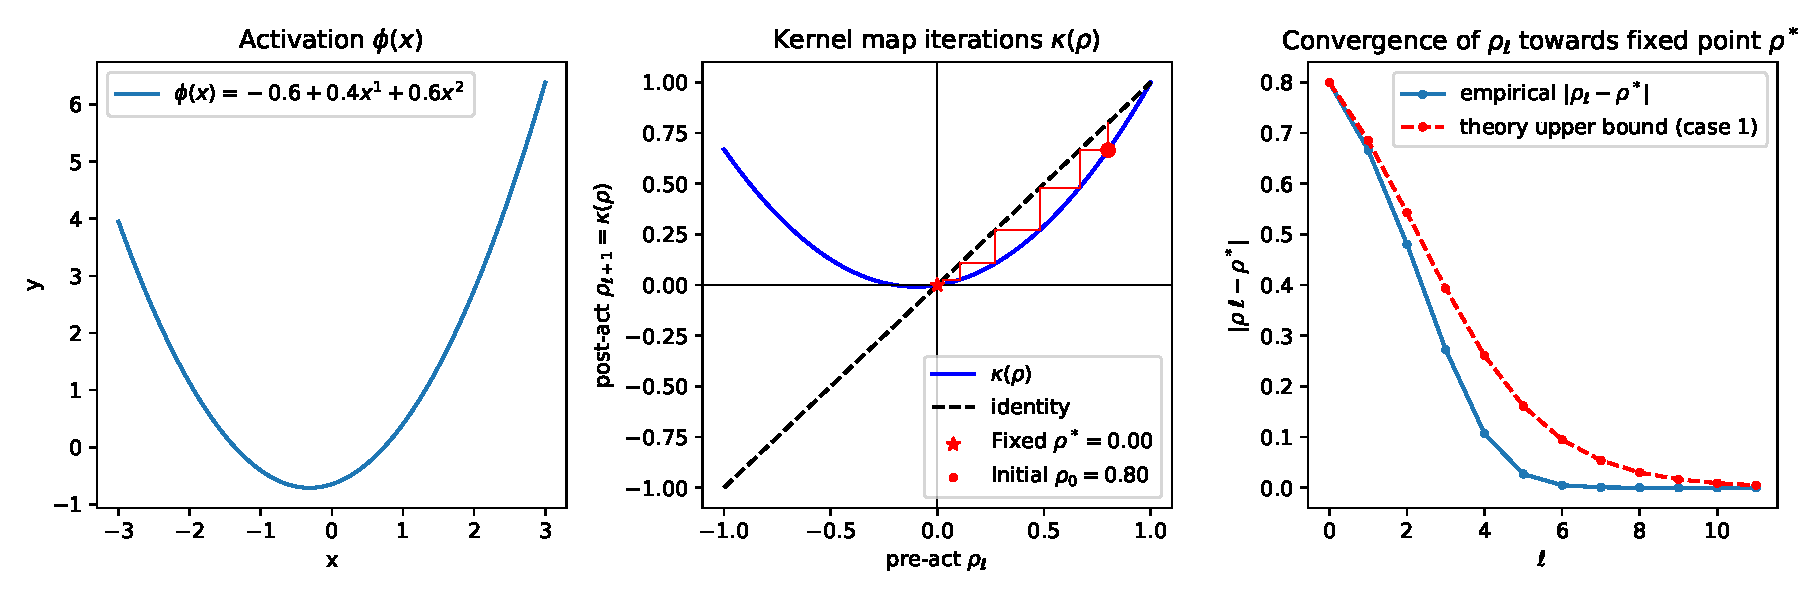
\includegraphics[width=\textwidth]{./kernel_map_convergence_case_0.pdf}
        \caption{\small Case 1}
    \end{subfigure}
    \hfill
    \begin{subfigure}[b]{0.7\textwidth}
        \centering
        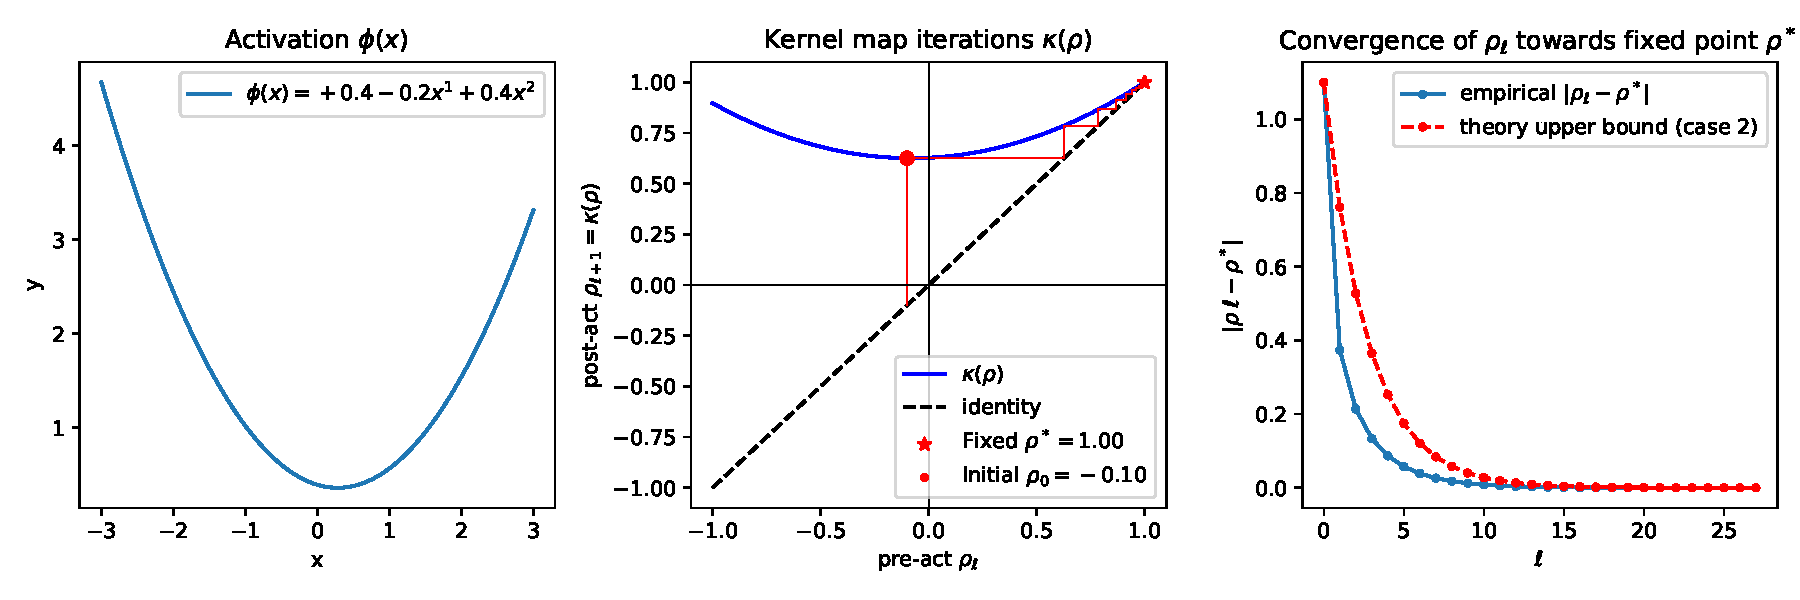
\includegraphics[width=\textwidth]{./kernel_map_convergence_case_1.pdf}
        \caption{\small Case 2}
    \end{subfigure}
    \\
    \begin{subfigure}[b]{0.7\textwidth}
        \centering
        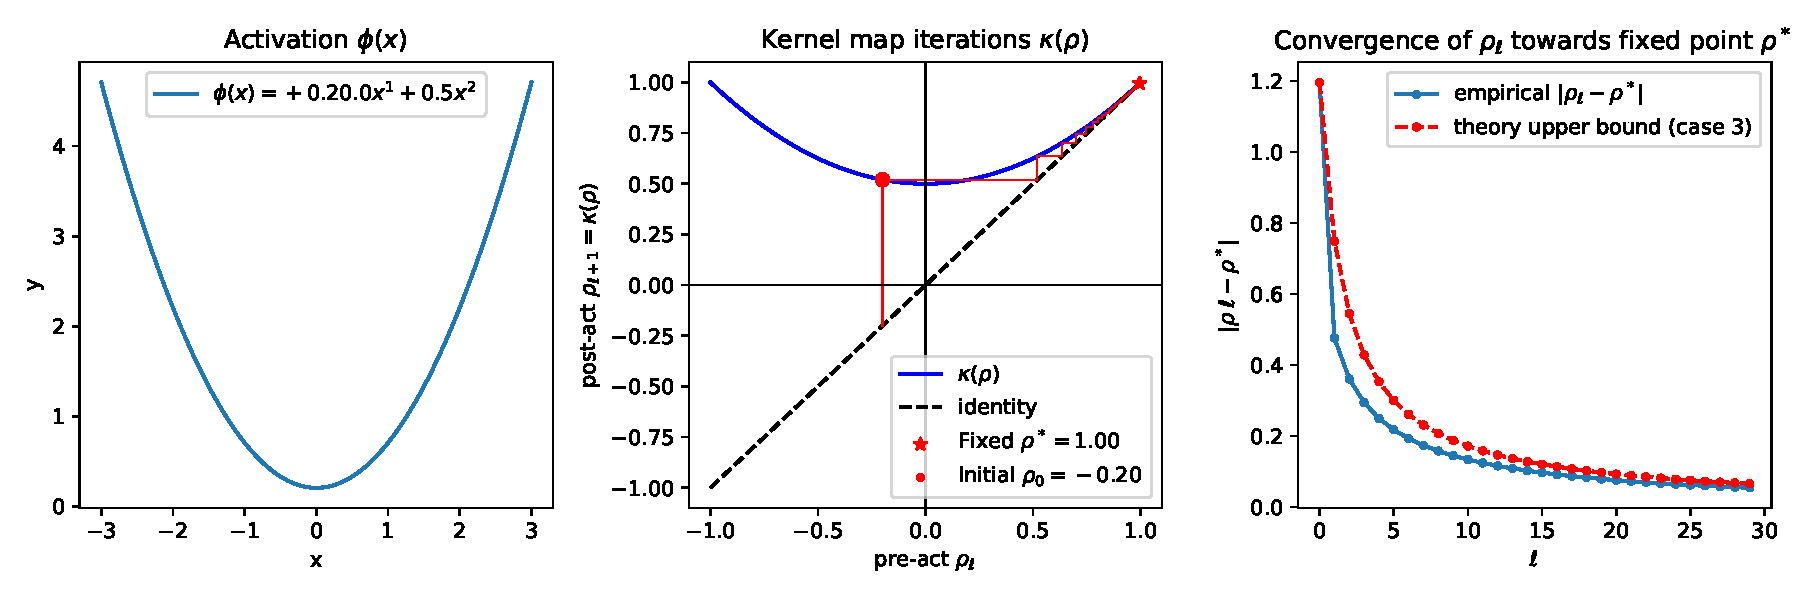
\includegraphics[width=\textwidth]{./kernel_map_convergence_case_2.pdf}
        \caption{\small Case 3}
    \end{subfigure}
    \hfill
    \begin{subfigure}[b]{0.7\textwidth}
        \centering
        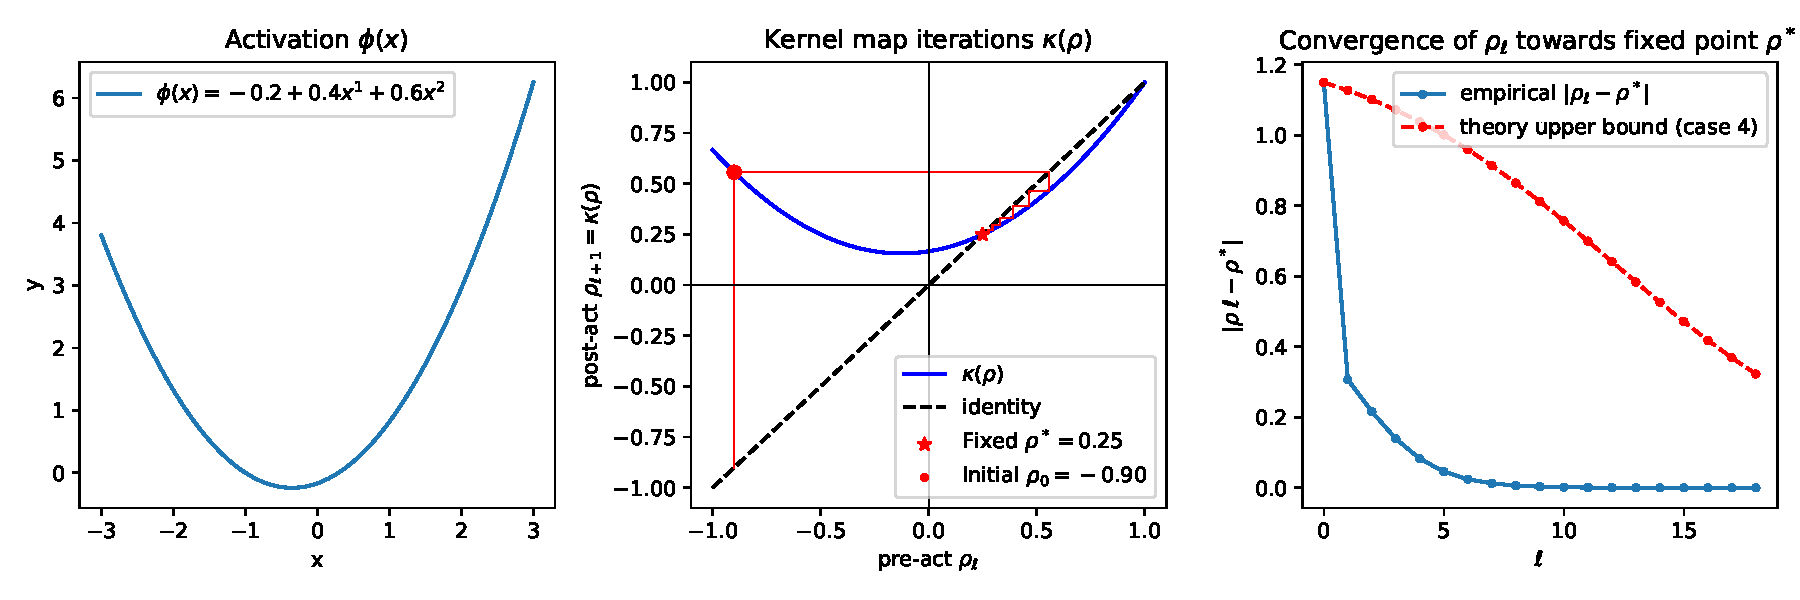
\includegraphics[width=\textwidth]{./kernel_map_convergence_case_3.pdf}
        \caption{\small Case 4}
    \end{subfigure}
    \caption{\small Validation of Theorem~\ref{iso:thm:global_attract}, each corresponding to one of the four cases of the theorem. Left column shows the activation $\phi.$ The middle and right columns show the kernel map show fixed point iteration starting from $\rho_0,$ and applying $\rho_{\ell+1}=\kappa(\rho_\ell)$ for many steps. The middle column shows the kernel map, while the right column shows the distance to the fixed point $\rho^*$.}
    \label{iso:fig:validation_plots}
\end{figure}

\begin{figure}[ht!]
    \centering
    \begin{subfigure}[b]{0.7\textwidth}
        \centering
        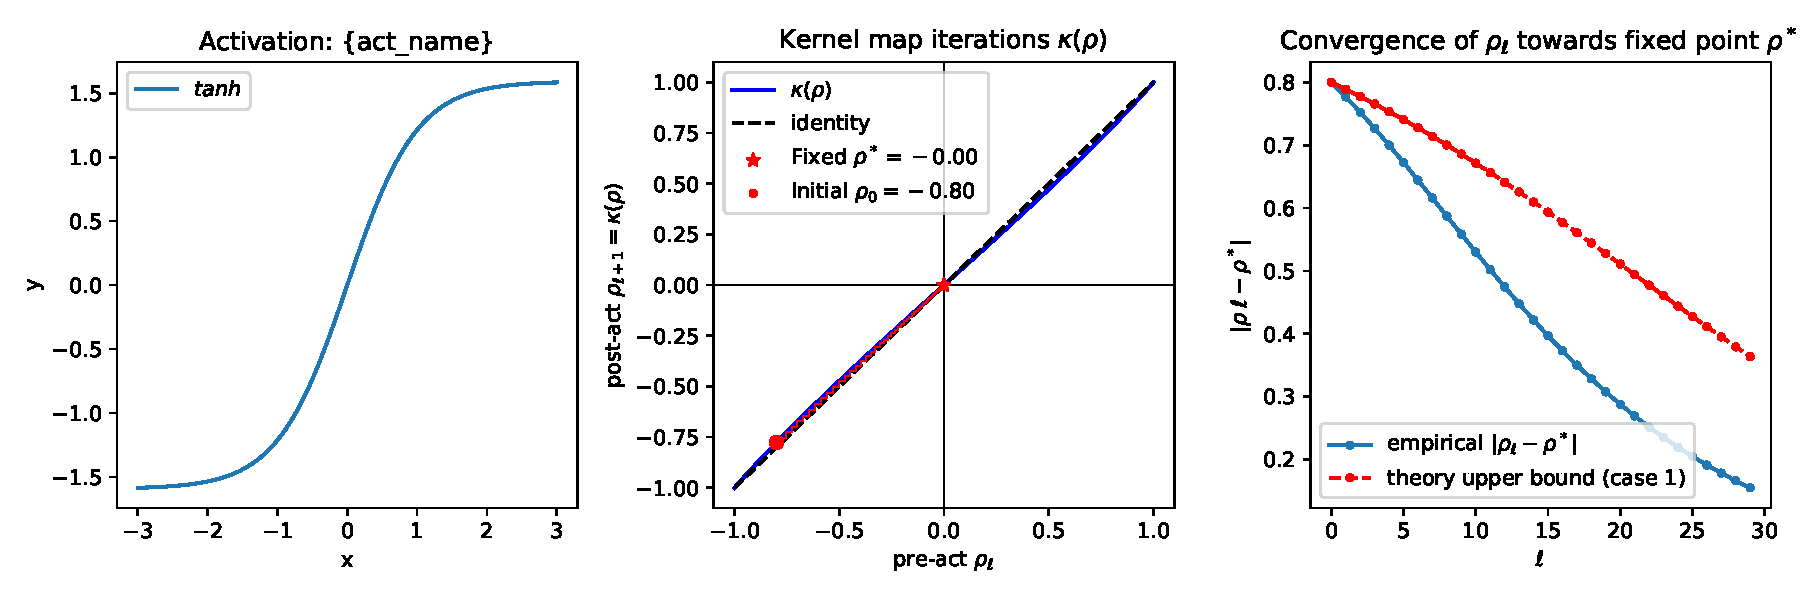
\includegraphics[width=\textwidth]{./kernel_map_convergence_case_0_tanh.pdf}
        \caption{\small Case 1. Tanh activation.}
    \end{subfigure}
    \hfill
    \begin{subfigure}[b]{0.7\textwidth}
        \centering
        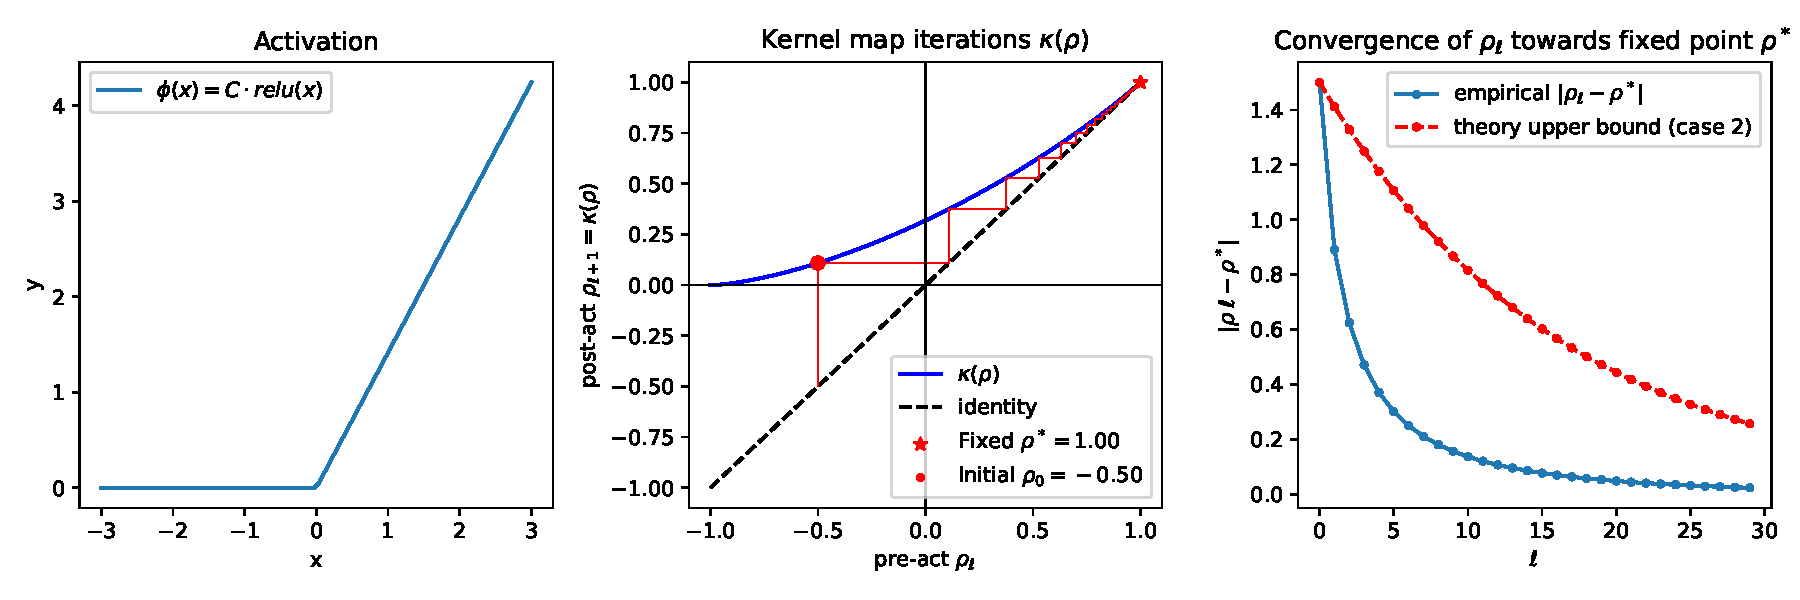
\includegraphics[width=\textwidth]{./kernel_map_convergence_case_1_relu.pdf}
        \caption{\small Case 2: ReLU activation.}
    \end{subfigure}
    \\
    \begin{subfigure}[b]{0.7\textwidth}
        \centering
        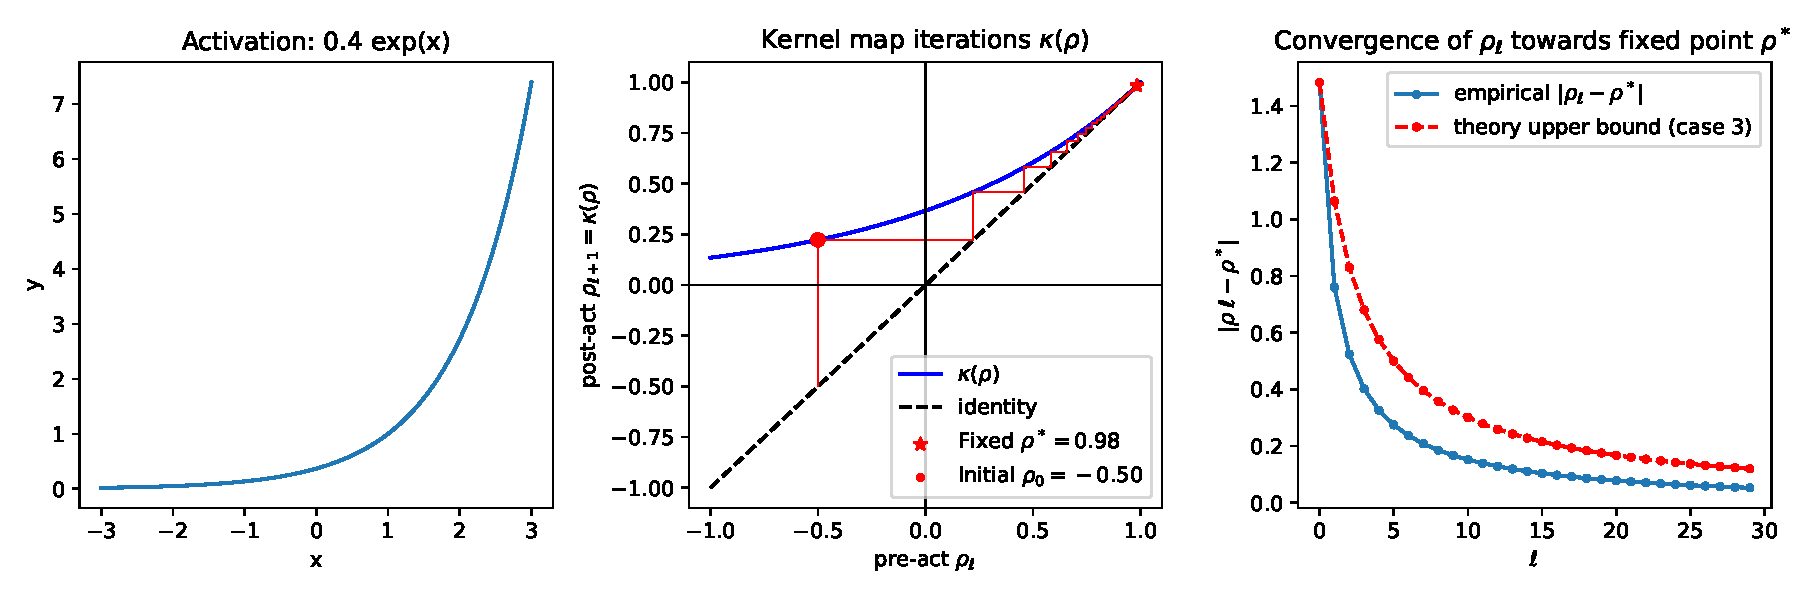
\includegraphics[width=\textwidth]{./kernel_map_convergence_case_2_exp.pdf}
        \caption{\small Case 3: Exponential activation.} 
    \end{subfigure}
    \hfill
    \begin{subfigure}[b]{0.7\textwidth}
        \centering
        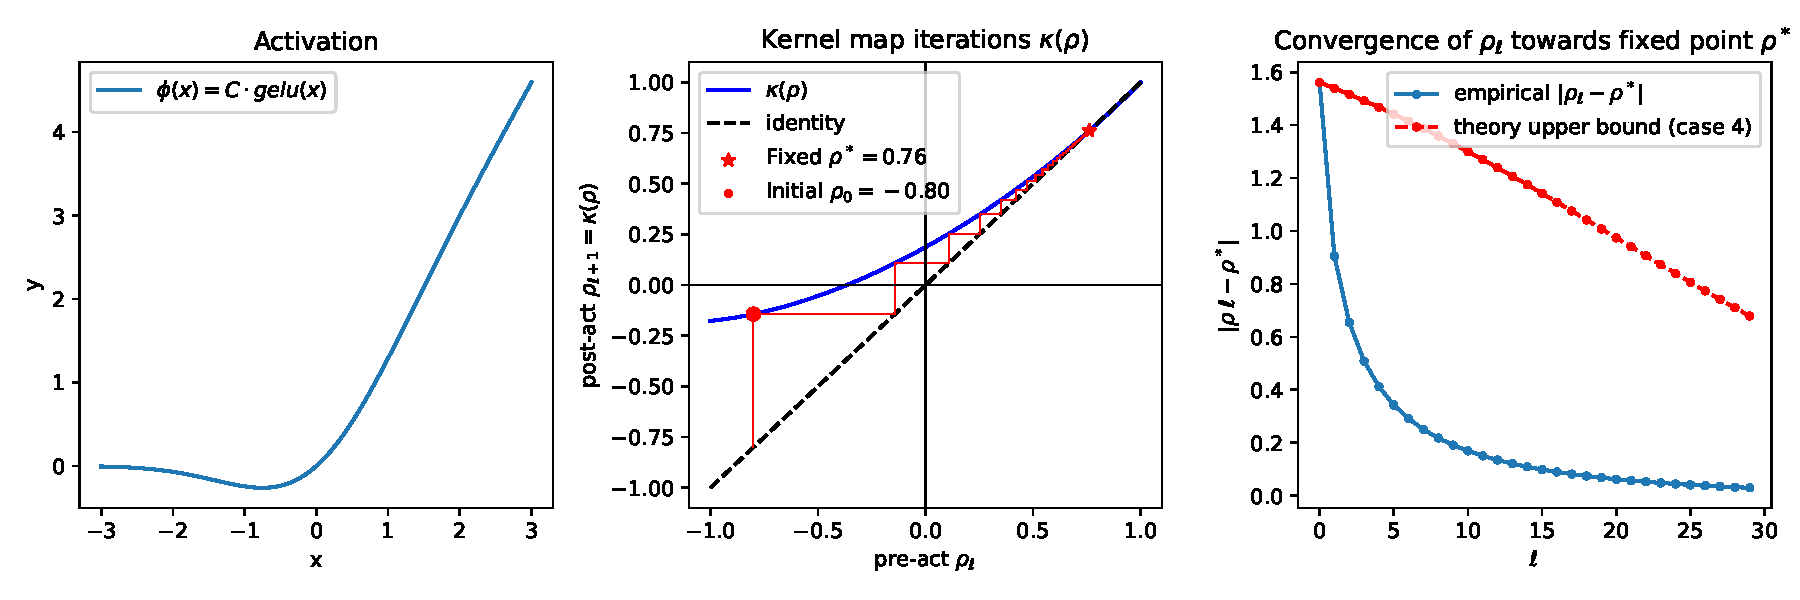
\includegraphics[width=\textwidth]{./kernel_map_convergence_case_3_gelu.pdf}
        \caption{\small Case 4: GELU activation.}
    \end{subfigure}
    \caption{\small Same as Figure~\ref{iso:fig:validation_plots} for some commonly used activations. }
    \label{iso:fig:validation_plots_real_activations}
\end{figure}




% \section{Stability in the non-mean field regime}
% So far, we only considered the mean field regime, where the state of every layer can be exactly determined by conditional expectation of the previous layer. However, when width $d$ is finite, because the sample and population means have some errors, it is not clear how the fixed points of the kernel map will behave. In this section, we will consider stability as the property that if the pre-activations have some deviation from the zero mean, unit variance Gaussian, the post-activations will still converge to the fixed point of the kernel map. In other words, we would like to find out the following dynamics, have locally or globally atracting fixed points:
% \begin{align}
% \mu_{\ell+1} = \E\; \phi(X),\ \sigma_{\ell+1}^2 = \text{Var}(\phi(X)), && X\sim N(\mu_\ell,\sigma_\ell^2),
% \end{align}
% where $\mu_0$ and $\sigma_0^2$ are the mean and variance of the input. Note that if we have centered and properly scaled activation $\E\phi(X)=0, \E\phi(X)^2 = 1,$ then $\mu=0,\sigma^2=1$ are the fixed points of the kernel map. However, in the finite width regime, we would like to know if the fixed points are locally or globally attractive.

% \begin{align}
% &\He_n(x+y) = \sum_{k=0}^n \binom{n}{k}x^{n-k} \He_k(y) \\
% &\He_n(\gamma x) = \sum_{i=0}^{\lfloor \frac{n}{2} \rfloor} \gamma^{n-2i} (\gamma^2 - 1)^i \binom{n}{2i} \frac{(2i)!}{i!} 2^{-i} \He_{n-2i}(x).
% \end{align}

% Thus if $\phi(x)=\sum_{k=0}^\infty c_k\He_k(x)$, for additive purturbation, we have 
% \begin{align*}
% \E_{X} \phi(X+\mu) &=  \E_X \sum_{n=0}^\infty c_n\He_n(X+\mu), && X\sim N(0,1)  \\
% &= \sum_{n=0}^\infty c_n \left(\E_X \sum_{k=0}^n \binom{n}{k}\mu^{n-k} \He_k(X)\right)\\
% &= \sum_{n=0}^\infty c_n \mu^n\\
% \end{align*}
% And for multiplicative purturbation, we have
% \begin{align*}
%     \E_{X} \phi(\gamma X)^2 &= \E_{X}\left(\sum_{n=0}^\infty c_n \He_n (\gamma X )\right)^2\\
%     &=  \E_X \left( \sum_{n=0}^\infty c_n \sum_{i=0}^{\lfloor \frac{n}{2} \rfloor} \gamma^{n-2i} (\gamma^2 - 1)^i \binom{n}{2i} \frac{(2i)!}{i!} 2^{-i} \He_{n-2i}(X)\right)^2\\
%     &= \E \left(\sum_n \He_n(X) \sum_{i=0}^\infty c_{n+2i}\gamma^{n}(\gamma^2-1)^i\binom{n+2i}{2i}\frac{2i!}{i! 2^i}\right)^2\\
%     &= \sum_{n=0}^\infty \left(\sum_{i=0}^\infty c_{n+2i}\gamma^{n}(\gamma^2-1)^i\binom{n+2i}{2i}\frac{2i!}{i! 2^i}\right)^2\E \He_n(X)^2\\
%     &= \sum_{n=0}^\infty n! \gamma^{2n}\left(\sum_{i=0}^\infty (\gamma^2-1)^i \binom{n+2i}{2i}\frac{2i!}{i! 2^i} c_{n+2i}\right)^2\\
%     &= \sum_{n=0}^\infty \sum_{k=0}^n \binom{n}{k}(\gamma^2-1)^k\sum_{i,j=0}^\infty (\gamma^2-1)^{i+j} \binom{n+2i}{2i}\frac{2i!}{i! 2^i}\binom{n+2j}{2j}\frac{2j!}{j! 2^j} c_{n+2j} c_{n+2i}\\
%     &= \sum_{n=0}^\infty \sum_{k=0}^n \binom{n}{k}\sum_{i,j=0}^\infty (\gamma^2-1)^{i+j+k} \binom{n+2i}{2i}\frac{2i!}{i! 2^i}\binom{n+2j}{2j}\frac{2j!}{j! 2^j} c_{n+2j} c_{n+2i}
% \end{align*}

% \section{Gradients and neural tangent kernel}
% So far, we only considered the forward passes. In this section, we consider the backward gradients, which will demosntate the importance of the convergence results that was established in the previous sections. 
% Before that, let us study a few elegant properties of Hermite polynomials that will be useful later.

% \begin{lemma}
% Let $\phi$ be an activation with Hermite expansion $\phi(z) = \sum_{k=0}^\infty c_k \he(z),$ and with kernel map $\kappa.$ Then, its derivative has Hermite expansion 
% \begin{align}
%     \phi'(z) = \sum_{k=1}^\infty \sqrt{k} c_k \he_{k-1}(z).
% \end{align}
%  Furthermore, if $X,Y$ are standard Gaussians with covariance $\rho,$ the kernel map of the derivative is given by 
% \begin{align}
% \E \phi'(X)\phi'(Y) = \kappa'(\rho)= \sum_{k=1}^\infty k c_k^2 \rho^{k-1}.
% \end{align}
% \end{lemma}

% This lemma shows a remarkable property of Hermite polynomilas, in that, the kernel map of derivative, is derivative of the kernel map of the original function. The main proof step is the fact that Hermite polynomials constitute an Appell sequence, i.e., $\He_k'(z) = \sqrt{k} \He_{k-1}(z).$ 

% \begin{proof}
% The derivative of probablist's Hermite polynomials is directly linked tho the lower degree Hermite polynomials, allowing us to write
% \begin{align*}
% \frac{d}{dz} \He_k'(z) = k \He_{k-1}(z) \\
% \implies \he_k'(z) = \sqrt{k} \he_{k-1}(z)\\
% \implies \phi'(z) = \sum_{k=1}^\infty \sqrt{k}c_k\he_{k-1}(z)
% \end{align*}
% Thus, we can conclude the proof by invoking Lemma~\ref{iso:lem:mehler_kernel}
% \begin{align*}
% \E \phi'(X)\phi'(Y) &= \E \left[\sum_{k=1}^\infty \sqrt{k} c_k \he_{k-1}(X) \sum_{k=1}^\infty \sqrt{k} c_k \he_{k-1}(Y) \right]\\
% &= \sum_{k=1,n=1}^\infty \sqrt{k} c_k \sqrt{n} c_n \E [\he_{k-1}(X)\he_{n-1}(Y)]  \\
% &=\sum_{k=1}^\infty k c_k^2 \E [\he_{k-1}(X)\he_{k-1}(Y)]^{k-1} && \text{Lemma~\ref{iso:lem:mehler_kernel}} \\
% &= \sum_{k=1}^\infty k c_k^2 \rho^{k-1} = \kappa'(\rho)
% \end{align*}

% \end{proof}

% Let us now consider the gradients of the MLPs

% \subsection{Gradients of MLPs}
% Given input dimension $d_0,$ output dimension $d_L,$ and hidden dimensions $d_1,\dots,d_{L-1},$ input $x\ni\R^{d_0}$ and output $y\in\R^{d_L},$ the MLP is defined as
% \begin{align*}
% &h^{0} := x, && x\in\R^{d_0}\\
% & z^\ell:=W_{\ell} h^{\ell-1}, && W_\ell\in\R^{d_{\ell}\times d_{\ell-1}},\text{drawn iid from }\sim N(0,1/d) \\
% &h^\ell := \phi(z^\ell), && \ell=1,\dots,L \\
% & \hat{y} := z^{L}=W_L h^{L-1}, && \hat{y},y\in\R^{d_L}
% \end{align*}
% Assuming sum squared, we can deinfe  
% \begin{align*}
% \mathcal{L}(x,y) &= \frac{1}{2} \|\hat{y} - y\|^2,
% \end{align*}
% the gradients of the last layer are given by
% \begin{align*}
% &\delta^{L}:=\frac{\partial \mathcal{L}}{\partial \hat{y}} = \hat{y} - y \\
% &\delta^\ell:=\frac{\partial \mathcal{L}}{\partial z^\ell}= \phi'(z^\ell)\odot (W_{\ell+1}^\top\delta^{\ell+1}), && \ell=1,\dots,L-1 \\
% &g^\ell:=\frac{\partial \mathcal{L}}{\partial W_\ell} = \delta^\ell\otimes h^{\ell-1}, && \ell=1,\dots,L,\\
% \end{align*}
% where $\otimes$ denotes the outer product, and the dependece of $\mathcal{L}$ and $\hat{y}$ on $x$ is omitted for brevity.



% The main goal of this section is to analyze the norm of the gradients in the mean field regime, and then to exend this to the Neural Tangent Kernel (NTK). In other words, we are interested in properties of $\|g^{l}\|_{rms},$ when $d_1,\dots,d_{L-1}\to \infty,$ and wether it vanishes or explodes with the depth of the network. For the NTK, we are interested in the properties of the sequence $\langle g^{l},g^{l}\rangle,$ when $d_1,\dots,d_{L-1}\to \infty.$

% In the remainder of this section, we will use $\rho_{X,Y}$ to refer to average inner product $\rho_{X,Y} = \frac1n \sum_{i=1}^n X_i^\top Y_i.$ Furthermore, we will use $\|X\|_{rms}$ to refer to the RMS norm $\frac1n \sum_{i=1}^n x_i^2.$

% % In this section, we are interested in the gradient norms 
% % \begin{align*}
% % &\text{delta and gradient norms} &&\|\delta^\ell\|_{rms}, \qquad \|g^\ell\|_{rms}, \\
% % &\text{delta similiarty} && \rho_{\delta_1^\ell,\delta_2^\ell}\\
% % &\text{gradient similarity} && \rho_{g_1^\ell,g_2^\ell},
% % \end{align*}
% % where in all cases, $\ell=0$ corresponds to input, and $\ell=L$ corresponds to the output layer, and the indices $1,2$ correspond to two different inputs. Also, recall from previous sections that given two inputs, the kernel sequence for two inputs is given by
% % \begin{align*}
% %     \rho^\ell_h:=\frac{\langle h_1^\ell,h^\ell_2\rangle}{\|h_1^\ell\|\|h_2^\ell\|},
% % \end{align*}
% % where $\ell=0$ corresponds two different inputs. 


% \begin{proposition}
%     Let $\phi$ be an activation that obeys $\E_{X\sim N(0,1)}\phi(X)^2=1.$ In the mean field regime, the norm of the gradients obeys
%     \begin{align}
%         \|\delta^\ell\|_{rms} = \|\delta^{\ell+1}\|_{rms} \kappa'(1)
%     \end{align}
%     Furthermore, for two inputs with initial similarity $\rho_0 = \langle x_1,x_2 \rangle $ the forward and backward passes follow recursion
%     \begin{align}
%         &\rho_\ell:=\rho_{h^\ell_1,h^\ell_2} = \kappa(\rho_{\ell-1})\\
%         &\langle \delta_1^\ell,\delta_2^\ell \rangle = \kappa'(\rho^\ell) \langle \delta_1^{\ell+1},\delta_2^{\ell+1} \rangle \\
%         &\langle g^\ell_1,g_2^\ell \rangle =\rho^{\ell-1}   \langle \delta_1^{\ell},\delta_2^{\ell} \rangle.
%     \end{align}
% \end{proposition}

% Let us consider the backward errors $\delta^{l}$ and their norms. Each index of $\delta^{l}$ is a Gaussian weights at layer $l+1$, by $\delta^{l+1}$ and $\phi'(z^{l}).$ Conditioned on the norm of $\delta^{l+1}$, with the independece of weights of at layer $l+1$ and pre-activations at layer $l$, norm of $\delta^{l}$ is the multiplication of norm of $\delta^{l+1}$ and the norm of $\phi'(z^{l}).$ Now, assuming that the activation is centered, pre-activations are standard Gaussian, and thus $\E \phi'(z^{l})^2 $ can be expanded based on the Hermite expansion and properties of Hermite polynomials 
% \begin{align*}
% &\phi'(z) = \sum_{k=1}^\infty c_k \he_{k-1}(z)\\
% &\E \phi'(z^{l})^2 = \sum_{k=1}^\infty \frac{c_k^2}{k}=:\beta\\
% &\|\delta^{l}\|_{rms} = \|\delta^{l+1}\|_{rms} \E \phi'(z^{l})^2 = \|\delta^{l+1}\|_{rms}\beta\\
% &\|\delta^{l}\|_{rms} = \|\delta^{L}\|_{rms} \beta^{L-l} = \|y-\hat{y}\|_{rms} \beta^{L-l}
% \end{align*}

% \begin{remark}
% Note that assuming that the activation unit second momnt $\E\phi(X)^2=1,$ we have $\sum_{k=1}^\infty c_k^2 = 1,$ which implies that $\beta \le 1.$ Furthermore, if the activation is non-linear, i.e., there is $c_k\neq 0$ for some $k\ge 2$, then the inequality is strict, i.e., $\beta < 1.$ 
% Recall that for the forward pass of an activation that centered and unit variance, we have shown the the kernel sequence converges towards zero with rate $\alpha = 1/(\sum_{k=1}c_k^2),$  where the rate becomes strict whenever we have any non-linearity. 
% This implies that the stronger the non-linearity, the faster the convergence of kernel sequence towards zero, and the faster the gradients norms converge towards zero. This shows that striking a balance between linearity and non-linearity is probably needed for a desirable initialization.
% \end{remark}


% Now, consider a generic layer $\delta' = \mathbf{W}^\top \delta \odot \phi'(\mathbf{z})$. Suppose $z_1,z_2 $ correspond to pre-activations for two different inputs, and $\delta_1,\delta_2$ are the corresponding gradients for previous and $\delta_1',\delta_2'$ are the gradients for the next layer. 

% If we look at one corresponding unit of $W_\top \delta_1$ and $W_\top \delta_2,$ they are jointly Gaussian with covariance $\E \delta_1\delta_2 .$ Thus, in the mean field, we can write
% \begin{align*}
%     \E \delta'_1\delta'_2 =  (\E \delta_1 \delta_2)(\E \phi'(z_1)\phi'(z_2)) 
%     = \E \delta_1\delta_2 f(\rho),
% \end{align*}
% where we used the fact that error-propagation vectors $\delta_1\delta_2$ are independent of pre-activations $z_1 z_2,$ because one relies on layers before and the other on layers after this step. 

% Now, in a multi-layer setting, let $r_l = \frac1d\langle \delta_1^{l},\delta_2^{l}\rangle$ denote the normalized inner product of the gradients at layer $l$, and let $\rho_\ell = \frac1d \langle z^{l}_1,z_2^{l}\rangle$ denote the normalized inner product of the pre-activations at layer $\ell$. Then, in the mean field regime, we have
% \begin{align*}
%     r_l = f(\rho_l) r_{l+1}
% \end{align*}
% Thus, for the weight gradients of layer $\ell$, we have


% \section{Limitations and open questions}

% The main theorem of this chapter, which was the global contraction towards zero, was only for the centered activations. However, there are possibly other fixed points. This question was not addressed in this chapter. 

% There is one conjecture that seems to be true but remained out of the scope of the results of this chapter:

% \begin{conjecture}
%     For any activation function $\phi$ that satisfies $\E_{X\sim N(0,1)}\phi(X) = 1,$ and is nonlinear, the following is true for the fixed-points of the kernel map :
%     \begin{itemize}
%         \item There are no fixed points in the range $(-1,0).$
%         \item There is exactly one fixed point in the range $\rho^*\in [0,1],$ that obeys $\kappa'(\rho^*) < 1,$ and it is globally attracting.
%     \end{itemize}
% \end{conjecture}



% \section{Implications for backward pass of MLPs}

% So far, we have only discussed the theory for the forward pass of neural networks. In this section, we will briefly discuss their implications for the backward pass. To the best of our knowledge, this connection has not been explored in the literature.

% \begin{proposition}
% Given an MLP with activation $\phi$ that has unit gain, in the mean field regime, the second moment of the eigenvalues of the Jacobian $J^\top J$ will be approximately $(\kappa'(1))^\ell$, which can be viewed as the backward gain of the activation function, $\kappa$ is the kernel map, and $\ell$ is the number of layers.
% \end{proposition}

% \begin{proof}
% Consider our principal result on the kernel map, which relates the covariance of pre-activations to the covariance of post-activations:

% \begin{align*}
% \kappa(\rho) = \E_{X,Y}[\phi(X)\phi(Y)] \quad \text{for } X,Y\sim \mathcal{N}(0,1) \text{ with covariance } \rho = \E[XY].
% \end{align*}

% Let us consider the scenario where the two signals are arbitrarily close, i.e., $\rho = 1- \epsilon$. In such a scenario, the kernel map  will be:

% \begin{align*}
% \lim_{\epsilon\to 0}\frac{\kappa(1)-\kappa(1-\epsilon)}{\epsilon} = \kappa'(1).
% \end{align*}

% This reveals that for a small $\epsilon$-perturbation in the covariance of pre-activations, the covariance of post-activations will be perturbed by $\kappa'(1)$-factor larger. We define this coefficient $\kappa'(1)$ as the backward gain of the activation function. In a multi-layer setting with $\ell$ layers, the gain will be $(\kappa'(1))^\ell$.

% Now, let's interpret this result using the definition of derivative. Consider an input $x$ and a small perturbation $\delta$. The output will be:
% \begin{align*}
% &h^\ell(x+\delta) = h^\ell(x) + J\delta, && J=\partial h^\ell(x)/\partial x,
% \end{align*}
% where $J$ is the input-layer-$\ell$ Jacobian. Thus, we can write:
% \begin{align*}
% \| h(x+\delta)-h(x)\| = \|J \delta\|.
% \end{align*}
% The backward gain in this sense will be $\|J \delta\|/\|\delta\|$.

% If we consider the case where the $\delta$ orientation is randomly chosen from a unit sphere, the distribution of $\|J \delta\|^2$ will be tightly related to the eigenvalue distribution of $J^\top J$. Specifically, its second moment will be:

% \begin{align*}
% \E_{\delta\sim \mathbf{S}^{d-1}} [\|J \delta\|^2] 
% = \frac1d \E_{\delta\sim \mathbf{S}^{d-1}} \sum_{i=1}^d \delta_{i}^2\lambda_i(J^\top J)\\
% =  \frac{1}{d} \sum_{i=1}^d \lambda_i(J^\top J).
% \end{align*}

% From our earlier analysis, we expect this quantity to be around $(\kappa'(1))^\ell$. Therefore, we can conclude that the second moment of the eigenvalues of $J^\top J$ will be approximately $(\kappa'(1))^\ell$, connecting our analysis of the backward pass to the Hermite expansion of the activation function.
% \end{proof}




% !TEX root = ../thesis-index.tex


\chapter{Batch normalization without gradient explosion}\label{ch:bn_grad}

% Wrote an alternative introduction
% \section{Introduction}
% \label{grad:sec:introduction}
\blfootnote{Code is available at: \url{https://github.com/alexandrumeterez/bngrad}}
%\paragraph{Training deep neural networks issues.}
What if we could train even deeper neural networks? Increasing depth empowers neural networks, by turning them into powerful data processing machines. For example, increasing depth allows large language models (LLMs) to capture longer structural dependencies~\citep{devlin2018bert,liu2019roberta,brown2020language,goyal2021larger,raffel2020exploring}. Also, sufficiently deep convolutional networks can outperform humans in image classification~\citep{liu2022convnet,woo2023convnext,wu2021cvt}. Nevertheless, increasing depth imposes an inevitable computational challenge: deeper networks are harder to optimize. In fact, standard optimization methods exhibit a slower convergence when training deep neural networks. Hence, computation has become a barrier in deep learning, demanding extensive research and engineering. 

A critical problem is that deeper networks suffer from the omnipresent issue of rank collapse at initialization: the outputs become collinear for different inputs as the network grows in depth~\citep{saxe2013exact}. Rank collapse is not only present in MLPs and convolutional networks~\citep{feng2022rank,saxe2013exact,daneshmand2020batch}, but also in transformer architectures~\citep{dong2021attention, noci2022signal}. This issue significantly contributes to the training slowdown of deep neural networks. Hence, it has become the focus of theoretical and experimental studies~\citep{saxe2013exact,feng2022rank,daneshmand2021batch,noci2022signal}.  

One of the most successful methods to avoid rank collapse is Batch Normalization (BN)~\citep{ioffe2015batch}, as proven in a number of theoretical studies ~\citep{yang2018a, daneshmand2020batch, daneshmand2021batch}. Normalization imposes a particular bias across the layers of neural networks~\citep{joudaki2023impact}. More precisely, the representations of a batch of inputs become more orthogonal after each normalization~\citep{joudaki2023impact}. This orthogonalization effect precisely avoids the rank collapse of deep neural networks at initialization~\citep{yang2018a,joudaki2023impact,daneshmand2021batch,joudaki2023bridging}. 

While batch normalization effectively avoids rank collapse, it causes numerical issues. The existing literature proves that batch normalization layers cause exploding gradients in MLPs in an activation-independent manner~\cite{yang2018a}. Gradient explosion limits increasing depth by causing numerical issues during backpropagation. For networks without batch normalization, there are effective approaches to avoid gradient explosion and vanishing, such as tuning the variance of the random weights based on the activation and the network width~\citep{he2015delving,glorot2010understanding}. However, such methods cannot avoid gradient explosion in the presence of batch normalization~\cite{yang2018a}. Thus, the following important question remains unanswered:  
\begin{center} \emph{Is there any network with batch normalization without gradient explosion and rank collapse issues?}\end{center}

\paragraph{Contributions.}
We answer the above question affirmatively by giving a specific MLP construction initialized with orthogonal random weight matrices, rather than Gaussian. To show that the MLP still has optimal signal propagation, we prove that the MLP output embeddings become isometric (\eqref{grad:eq:iso_gap}), implying the output representations becomes more orthogonal with depth. For a batch of linearly independent inputs, we prove
\begin{align}\label{grad:eq:iso_gap_decay}
    \E\big[\text{isometry gap}\big] = \mathcal{O}\left( e^{-\text{depth}/C}\right),
\end{align}
where $C$ is a constant depending only on the network width and input and the expectation is taken over the random weight matrices. Thus, for sufficiently deep networks, the representations rapidly approach an orthogonal matrix. While \citet{daneshmand2021batch} prove that the outputs converge to within an $\mathcal{O}(\text{width}^{-1/2})$-ball close to orthogonality, we prove that the output representations become perfectly orthogonal in the infinite depth limit. This perfect orthogonalization turns out to be key in proving our result about avoiding gradient explosion. In fact, for MLPs initialized with Gaussian weights and BN, \citet[Theorem 3.9]{yang2018a} prove that the gradients explode at an exponential rate in depth. In a striking contrast, we prove that gradients of an MLP with BN and orthogonal weights remain bounded as
\begin{align}\label{grad:eq:grad_norm_bounded}
    \E \big[
\log\left(\text{gradient norm for each layer}\right)\big] = \mathcal{O}\left( \text{width}^5\right).
\end{align}
Thus, the gradient is bounded by a constant that only depends on the network width where the expectation is taken over the random weight matrices. It is worth noting that both isometry and log-norm gradient bounds are derived \emph{non-asymptotically}. Thus, in contrast to the previously studied mean field or infinite width regime, our theoretical results hold in practical settings where the width is finite. 

The limitation of our theory is that it holds for a simplification in the BN module and linear activations. However, our results provide guidelines to avoid gradient explosion in MLPs with non-linear activations. We experimentally show that it is possible to avoid gradient explosion for certain non-linear activations with orthogonal random weights together with ``activation shaping''~\cite{martens2021rapid}. Finally, we experimentally demonstrate that avoiding gradient explosion stabilizes the training of deep MLPs with BN. 

\section{Related work}
\label{grad:sec:related_work}
\paragraph{The challenge of depth in learning.} Large depth poses challenges for the optimization of neural networks, which becomes slower by increasing the number of layers. This depth related slowdown is mainly attributed to: (i) gradient vanishing/explosion, and (ii) the rank collapse of hidden representations. (i) Gradient vanishing and explosion is a classic problem in neural networks ~\citep{hochreiter1998vanishing}. For some neural architectures, this issue can be effectively solved. For example, \citet{he2015delving} propose a particular initialization scheme that avoids gradient vanishing/explosion for neural networks with rectifier non-linearities while  \citet{glorot2010understanding} study the effect of initialization on sigmoidal activations. However, such initializations cannot avoid gradient explosion for networks with batch normalization~\citep{yang2018a,lubana2021beyond}. (ii) \citet{saxe2013exact} demonstrate that outputs become independent from inputs with growing depth, which is called the rank collapse issue~\citep{daneshmand2020batch,dong2021attention}. Various techniques have been developed to avoid rank collapse such as batch normalization~\cite{ioffe2015batch}, residual connections~\cite{he2016res}, and self-normalizing activations~\cite{klambauer2017self}. A related line of work has shown how signal propagation can be achieved without batch normalization in feed-forward networks ~\citep{burkholz2019initialization} and ResNets~\citep{brock2021characterizing}.
Other works on CNNs~\cite{blumenfeld2020beyond} have shown that symmetry breaking is a vital element for achieving signal propagation with stable gradients in deep models. 
Here, we focus on batch normalization since our primary goal is to avoid the systemic issue of gradient explosion for batch normalization.

\paragraph{Initialization with orthogonal matrices.}
\citet{saxe2013exact} propose initializing the weights with random orthogonal matrices for linear networks without normalization layers. Orthogonal matrices avoid the rank collapse issue in linear networks, thereby enabling a depth-independent training convergence. \citet{pennington2017resurrecting} show that MLPs with sigmoidal activations achieve dynamical isometry when initialized with orthogonal weights. Similar benefits have been achieved by initializing CNNs with orthogonal or almost orthogonal kernels~\citep{xiao2018dynamical,mishkin2015all}, and by initializing RNN transition matrices with elements from the orthogonal and unitary ensembles ~\citep{arjovsky2016unitary,le2015simple,henaff2016recurrent}. Similarly, we use orthogonal random matrices to avoid gradient explosion. What sets our study apart from this literature is that our focus is on batch normalization and the issue of gradient explosion.

\paragraph{Networks with linear activation functions.}
Due to its analytical simplicity, the identity function has been widely used in theoretical studies for neural networks. Studies on identity activations date back to at least two decades. \citet{fukumizu1998effect} studies batch gradient descent in linear neural networks and its effect on overfitting and generalization. \citet{baldi1995learning} provide an overview over various theoretical manuscripts studying linear neural networks. Despite linearity, as \citet{saxe2013exact, saxe2013learning} observe, the gradient dynamics in a linear MLP are highly nonlinear. In a line of work,  \citet{saxe2013learning,saxe2013exact, saxe2019mathematical} study the training dynamics of deep neural networks with identity activations and introduce the notion of dynamical isometry. \citet{baldi1989neural} and \citet{yun2017global} study the mean squared error optimization landscape in linear MLPs. More recently, the optimum convergence rate of gradient descent in deep linear neural networks has been studied by \citet{arora2018convergence} and \citet{shamir2019exponential}. \citet{du2019width} prove that under certain conditions on the model width and input degeneracy, linear MLPs with Xavier initialized weights~\citep{glorot2010understanding} converge linearly to the global optimum. Akin to these studies, we also analyze networks with linear activations. However, batch normalization is a non-linear function, hence the network we study in this chapter is a highly non-linear function of its inputs.

\paragraph{Mean field theory for random neural networks.} 
The existing analyses for random networks often rely on mean field regimes where the network width tends to infinity~\citep{pennington2017resurrecting,yang2018a,li2022neural,pennington2017nonlinear}. However, there is a discrepancy between mean field regimes and the practical regime of finite width. While some analyses attempt to bridge this gap~\citep{joudaki2023bridging,daneshmand2021batch}, their results rely on technical assumptions that are hard to validate. In contrast, our non-asymptotic results hold for standard neural networks used in practice. Namely, our main assumption for avoiding rank collapse and gradient explosion is that samples in the input batch are not linearly dependent, which we will show is necessary. To go beyond mean field regimes, we leverage recent theoretical advancements in Weingarten calculus~\citep{weingarten1978asymptotic, collins2003moments, banica2011polynomial, collins2006integration, collins2022weingarten}.


\paragraph{Mean field theory for random neural networks.}\label{grad:sec:supp_rel_work}
The existing analyses for random networks often rely on mean field regimes where the network width tends to infinity~\citep{pennington2017resurrecting,yang2018a,li2022neural,pennington2017nonlinear}. However, there is a discrepancy between mean field regimes and the practical regime of finite width. While some analyses attempt to bridge this gap~\citep{joudaki2023bridging,daneshmand2021batch}, their results rely on technical assumptions that are hard to validate. In contrast, our non-asymptotic results hold for standard neural networks used in practice. Namely, our main assumption for avoiding rank collapse and gradient explosion is that samples in the input batch are not linearly dependent, which we will show is necessary. To go beyond mean field regimes, we leverage recent theoretical advancements in Weingarten calculus~\citep{weingarten1978asymptotic, collins2003moments, banica2011polynomial, collins2006integration, collins2022weingarten}.

% \input{sections/main_new}
\section{Main results} \label{grad:sec:main}
We will develop our theory by constructing networks that do not suffer from gradient explosion~(Sec.~\ref{grad:sec:explosion}) and still orthogonalize~(Sec.~\ref{grad:sec:orthogonality}). The construction is similar to the network studied by  \citet{daneshmand2021batch}: an MLP with batch normalization and linear activations. Formally, let $X^\ell \in \R^{d\times n}$ denote the representation of $n$ samples in $\R^d$ at layer $\ell$, then
\begin{align}
    X_{\ell+1} = \BN(W_\ell X_{\ell}), && \ell=0, \dots, L \label{grad:eqn:mlp_def},
\end{align}
where $W_\ell \in \R^{d\times d}$ are random weights, $n$ is the mini-batch size and $d$ is the feature dimension. Analogous to recent theoretical studies of batch normalization~\citep{daneshmand2021batch,daneshmand2020batch}, we define the BN operator $\BN: \R^{d \times n} \to \R^{d \times n}$ as 
\begin{align}
    \BN(X) &= \diag(XX^\top)^{-\frac{1}{2}}X, \quad \BN(X)_{ij} = \frac{X_{ij}}{\sqrt{\sum_{k=1}^d X_{ik}^2}}~.
    \label{grad:eqn:bn_def}
\end{align}
Note that compared to the standard BN operator, mean reduction in \eqref{grad:eqn:bn_def} is omitted. Our motivation for this modification, similar to \citet{daneshmand2021batch}, is purely technical and to streamline our theory. We will experimentally show that using standard BN modules instead does not influence our results on gradient explosion and signal propagation (for more details see Figure~\ref{grad:fig:mean_reduction}). A second minor difference is that in the denominator, we have omitted a $\frac1n$ factor. However, this only amounts to a constant scaling of the representations and does not affect our results. 

Compared to \citet{daneshmand2021batch}, we need two main modifications to avoid gradient explosion: (i) $n=d$, and (ii) $W_\ell$ are random \emph{orthogonal} matrices. More precisely, we assume the distribution of $W_\ell$ is the Haar measure over the orthogonal group denoted by $\mathbb{O}_d$ ~\citep{collins2006integration}. Such an initialization scheme is widely used in deep neural networks without batch normalization~\citep{saxe2013exact,xiao2018dynamical,pennington2017resurrecting}. For MLP networks with BN, we prove such initialization avoids the issue of gradient explosion, while simultaneously orthogonalizing the inputs.

\subsection{Tracking signal propagation via orthogonality}
\label{grad:sec:orthogonality}
As discussed, batch normalization has an important orthogonalization bias that influences training. Without normalization layers, representations in many architectures face the issue of rank-collapse, which happens when network outputs become collinear for arbitrary inputs, hence their directions become insensitive to the changes in the input. In contrast, the outputs in networks with batch normalization become increasingly orthogonal through the layers, thereby enhancing the signal propagation in depth~\cite{daneshmand2021batch}. Thus, it is important to check whether the constructed network maintains the important property of orthogonalization. 

\paragraph{Isometry gap.}
Our analysis relies on the notion of \emph{isometry gap}, $\IG: \R^{d\times n} \to \R$, introduced by \citet{joudaki2023impact}. Isometry gap is defined as
\begin{align}\label{grad:eq:iso_gap}
 \IG(X) = -\log \left(\frac{\det(X^\top X)^{\frac{1}{d}} }{\frac{1}{d}\tr(X^\top X)} \right). 
\end{align}
One can readily check that $\IG(X) \geq 0$ and it is zero when $X$ is an orthogonal matrix, i.e., $X X^\top = I_d$. The \emph{isometry} denoted by $\I:\R^{d\times n} \to \R$ is defined as $\I(X) = \exp(-\IG(X))$. 

\begin{figure}[ht]
    \centering
    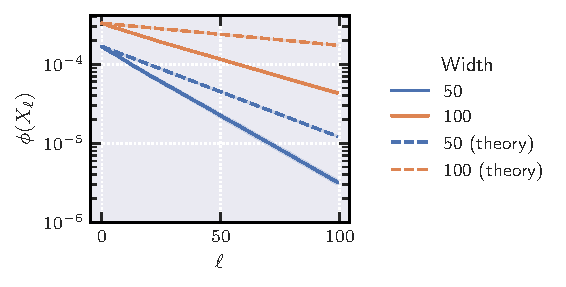
\includegraphics[width=0.7\textwidth]{figures/intro_figure_isogap.pdf}
    \caption{Isometry gap (y-axis, log-scale) in depth for an MLP with orthogonal weights, over randomly generated data. As predicted by Theorem~\ref{grad:thm:iso_gap_decay_in_depth}, isometry gap of representations vanishes at an exponential rate. The solid traces are averaged over $10$ independent runs, and the dashed traces show the theoretical prediction from Theorem~\ref{grad:thm:iso_gap_decay_in_depth}.}
    \label{grad:fig:linear_contrast} 
\end{figure}

\paragraph{Geometric interpretation of isometry.}
While the formula for isometry gap may seem enigmatic at first, it has a simple geometric interpretation that makes it intuitively understandable. The determinant $\det(X^\top X) = \det(X)^2$ is the squared volume of the parallelepiped spanned by the columns of $X$, while $\tr(X^\top X)$ is the sum squared-norms of the columns of $X$. Thus, the ratio between the two provides a scale-invariant notion of volume and isometry. On the one hand, if there is any collinearity between the columns, the volume will vanish and the isometry gap will be infinity, $\psi(X) = \infty$. On the other hand, $\psi(X) = 0$ implies $X^\top X$ is a scaled identity matrix. We will prove $\psi$ serves as a Lyapunov function for the chain of hidden representations $\{X_\ell\}_{\ell=0}^\infty$.

\paragraph{Theory for orthogonalization.}
The following theorem establishes the link between orthogonality of representations and depth. 
\begin{theorem}
\label{grad:thm:iso_gap_decay_in_depth}
There is an absolute constant $C$ such that for any layer $\ell \leq L$ we have
\begin{align}
    &\E \IG(X_{\ell+1})\le \IG(X_0)e^{-\ell/k}, & \text{where}&& k:=Cd^2(1+ d\IG(X_0))~.
\end{align}
\end{theorem}



Theorem~\ref{grad:thm:iso_gap_decay_in_depth} states that if the samples in the input batch are not linearly dependent, representations approach orthogonality at an exponential rate in depth. The orthogonalization in depth ensures the avoidance of the rank collapse of representations, which is a known barrier to training deep neural networks~\cite{daneshmand2020batch,saxe2013exact,bjorck2018understanding}. 

Figure~\ref{grad:fig:linear_contrast}
compares the established theoretical decay rate of $\psi$ with the practical rate. Interestingly, the plot confirms that the rate depends on width in practice, akin to the theoretical rate in Theorem~\ref{grad:thm:iso_gap_decay_in_depth}. It is worth mentioning that the condition on the input samples to not be linearly dependent is necessary to establish this result. One can readily check that starting from a rank-deficient input, neither matrix products, nor batch-normalization operations can increase the rank of the representations. Since this assumption is quantitative, we can numerically verify it by randomly drawing many input mini-batches and check if they are linearly dependent. For CIFAR10, CIFAR100, MNIST and FashionMNIST, we empirically tested that most batches across various batch sizes are full-rank (see Section~\ref{grad:sec:datasets_independence} for details on the average rank of a batch in these datasets). 

Theorem~\ref{grad:thm:iso_gap_decay_in_depth} distinguishes itself from the existing orthogonalization results in the literature~\citep{yang2018a,joudaki2023impact} as it is non-asymptotic and holds for networks with finite width. Since practical networks have finite width and depth, non-asymptotic results are crucial for their applicability to real-world settings. While \citet{daneshmand2021batch} provide a non-asymptotic bound for orthogonalization, the main result relies on an assumption that is hard to verify. 


\textit{Proof idea of Theorem~\ref{grad:thm:iso_gap_decay_in_depth}.}
We leverage a recent result established by  \citet{joudaki2023impact}, proving that the isometry gap does not decrease with BN layers. 
For all non-degenerate matrices $X \in \R^{d \times d}$, the following holds
    \begin{align*}
        \I(\BN(X))\geq \left(1+ \frac{\mathrm{variance}\{\|X_{j\cdot}\|\}_{j=1}^d}{(\mathrm{mean} \{\|X_{j\cdot}\|\}_{j=1}^d)^2}\right) \I(X)~.
    \end{align*}
Using the above result, we can prove that matrix multiplication with orthogonal weights also does not decrease isometry as stated in the next lemma. 
\begin{lemma}[Isometry after rotation]
\label{grad:lem:iso_rotation}
Let $X \in \R^{d\times d}$ and $W \in \R^{d\times d}$ be an orthogonal matrix and $X' = W X$; then,  
\begin{align}
   \I(\BN(X'))\geq \left(1+ \frac{\mathrm{variance}\{\|X'_{j\cdot}\|\}_{j=1}^d}{(\mathrm{mean} \{\|X'_{j\cdot}\|\}_{j=1}^d)^2}\right) \I(X)~.
\end{align}
\end{lemma}
%
It is straightforward to check that there exists at least an orthogonal matrix $W$ for which $\I(\BN(WX))=1$ (see Corollary~\ref{grad:cor:isometry_increase}). Thus, $\I(\cdot)$ strictly increases for some weight matrices, as long as $X$ is not orthogonal. When the distribution of $W$ is the Haar measure over the orthogonal group, we can leverage recent developments in Weingarten calculus~\citep{weingarten1978asymptotic, banica2011polynomial,collins2006integration,collins2022weingarten} to calculate a rate for the isometry increase in expectation: 
\begin{theorem}
    \label{grad:thm:iso_bound}
    Suppose $W \sim \mathbb{O}_d$ is a matrix drawn from $\mathbb{O}_d$ such that the distribution of $W$ and $UW$ are the same for all orthogonal matrices $U$. Let $\{\lambda_i\}_{i=1}^d$ be the eigenvalues of $XX^\top$. Then,
    % \begin{align}
    %     \E_W \left[\I(\BN(WX))\right ] \geq \left( \frac{1}{ 1 - \frac{\sum_{k=1}^d (\lambda_k - 1)^2}{2d^2(d+2)} } \right) \I(X)   
    % \end{align}
    \begin{align}
        \E_W \left[\I(\BN(WX))\right ] \geq \left( 1 - \frac{\sum_{k=1}^d (\lambda_k - 1)^2}{2d^2(d+2)} \right)^{-1} \I(X)   
    \end{align}
    holds for all $X = \BN(\cdot)$, with equality for orthogonal matrices.
\end{theorem}
The structure in $X$ induced by \BN{} ensures its eigenvalues lie in the interval $(0,1]$, in that the multiplicative factor in the above inequality is always greater than one. In other words, $\I(\cdot)$ increases by a constant factor in expectation that depends on how close $X$ is to an orthogonal matrix. 

The connection between Theorem~\ref{grad:thm:iso_bound} and the main isometry gap bound stated in Theorem~\ref{grad:thm:iso_gap_decay_in_depth} is established in the following Corollary (recall $\psi = -\log \I$). 

\begin{corollary}[Isometry gap bound]
% \label{grad:cor:isogap_bound}
Suppose the same setup as in Theorem~\ref{grad:thm:iso_bound}, where $X' = WX$. Then, we have:
\begin{align}
    \E_W[\IG(X') | X] \leq \IG(X) + \log \left(1 - \frac{\sum_k(\lambda_k - 1)^2}{2d^2(d+2)}\right).
\end{align}

  

\end{corollary}
  Notice that the term $\frac{\sum_{k=1}^d (\lambda_k - 1)^2}{2d^2(d+2)} = \mathcal{O}(\frac{1}{d})$, yielding $\log\left[1 - \frac{\sum_{k=1}^d (\lambda_k - 1)^2}{2d^2(d+2)} \right] \leq 0$.

% Finally, we establish the connection between the isometry bound and the isometry gap bound stated in Theorem~\ref{grad:thm:iso_gap_decay_in_depth} in Corollary~\ref{grad:cor:isogap_bound}. 
The rest of proof is based on an induction over the layers, presented in Appendices~\ref{grad:sec:conditional_orthonality} and~\ref{grad:sec:proof_isometry_depth}.  
% \end{itemize}
% \end{proof}

\subsection{Orthogonalization and gradient explosion}
There is a subtle connection between orthogonalization and gradient explosion. Suppose the input batch is rank-deficient, i.e., degenerate. As elaborated above, since all operations in our MLP can be formulated as matrix products, they cannot recover the rank of the representations, which thus remain degenerate. By perturbing the input such that it becomes full-rank, the output matrix becomes orthogonal, hence non-degenerate at an exponential rate in depth as proven in Theorem~\ref{grad:thm:iso_gap_decay_in_depth}. 

\begin{figure}[ht]
    \centering
    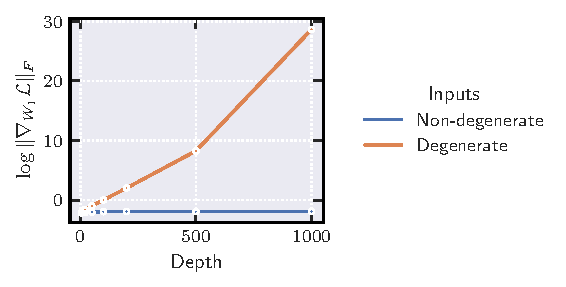
\includegraphics[width=0.7\textwidth]{figures/log_degenerate_inputs.pdf}
    \caption{Logarithmic plot for the gradient norm of the first layer for networks with different number of layers evaluated on degenerate (orange) and non-degenerate (blue) inputs. The degenerate inputs contain repeated samples from CIFAR10 in the batch, measured at initialization for MLPs of various depths. While gradients explode for degenerate inputs, there is no explosion for non-degenerate inputs. Traces are averaged over $10$ independent runs.}
    \label{grad:fig:degenerate_input}
\end{figure}
Thus, a slight change in inputs leads to a significant change in outputs from degeneracy to orthogonality. Considering that the gradient measures changes in the loss for infinitesimal inputs changes, the large changes in outputs potentially lead to gradient explosion. While this is only an intuitive argument, we observe that in practice the gradient does explode for degenerate inputs, as shown in Figure~\ref{grad:fig:degenerate_input}. 

Nonetheless, in Figure~\ref{grad:fig:degenerate_input} we observe that for non-degenerate inputs the gradient norm does not explode. In fact, we observe that inputs are often non-degenerate in practice (see Table~\ref{grad:tab:batch_degen} for details). Thus, an important question is whether the gradient norm remains bounded for non-degenerate input batches. Remarkably, we can not empirically verify that for \emph{all degenerate inputs} the gradient norm remains bounded. Therefore, a theoretical guarantee is necessary to ensure avoiding gradient explosion. 

% However, in Figure~\ref{grad:fig:degenerate_input},  we observe that for non-degenerate inputs the gradient norm does not explode. Since we observed that inputs often are non-degenerate in practice \alex{(see Table~\ref{grad:tab:batch_degen} for more details)} \hadi{reference?},  it is important to analyze the gradient norm for non-degenerate matrix. Notably, we can not empirically check the gradient norm explosion for all non-degenerate input matrices. Indeed, theory is a \emph{necessity} here but not a choice. Gradient explosion for a single non-degenerate input would cause numerical issues in training.  This motivates our theoretical analysis for gradient norm in the next section. 
% \begin{figure}[ht]
%     \centering
%     \includegraphics[width=0.6\linewidth]{figures/plots/degenerate_inputs.pdf}
%     \caption{Gradient explosion in depth for degenerate (orange) and non-degenerate (blue) inputs, where the degenerate inputs contain repeated samples in the batch, measured at initialization for MLPs of various depths. Degenerate inputs explode at an exponential rate in depth. Curves are averaged over $10$ independent runs, with the shaded region showing the $95\%$ confidence interval %\hadi{remove 20\% plot. Replace Gaussian with non-degenerate inputs and blue with degenerate inputs. Remove titles of 80\% on top. Replace initialization in the legend with inputs. We can also move it to the appendix}.\amir{Agreed.}}
%     }
%     \label{grad:fig:degenerate_input}
% \end{figure}



\subsection{Avoiding gradient explosion in depth}
\label{grad:sec:explosion}
So far, we have proven that the constructed network maintains the orthogonalization property of BN. Now, we turn our focus to the gradient analysis. The next theorem proves that the constructed network does not suffer from gradient explosion in depth for non-degenerate input matrices. 

\begin{theorem}\label{grad:thm:no_explosion}
Let the loss function $\Loss: \R^{d \times d} \to \R$ be $\mathcal{O}(1)$-Lipschitz, and input batch $X_0$ be non-degenerate. Then, there exists an absolute constant $C$ such that for all $\ell \leq L$ it holds
% \begin{align}
%     \E \left[ \log \| \nabla_{W_\ell} \mathcal{L}(X_\ell)\|\right] \le C d^5 \psi(X_0) \left(1 - e^{-L/k}\right), && k = C d^3(1+d\psi(X_0))
% \end{align}
\begin{align}
    \E \left[ \log \| \nabla_{W_\ell} \mathcal{L}(X_\ell)\|\right] \leq  Cd^5 (\psi(X_0)^3 + 1)
\end{align}

% \hadi{Is it possible to put theorem in one column. This is our main result and need more space. Figure 2 should be in section 3.2 somehow}
% \alex{yes, I'll reorder and fix spacing once we converge on the language and what versions of lemmas we leave in the main body} 
% \begin{align*}\tag{small isogap}
%     \E \left[ \log \| \nabla_{W_\ell} \mathcal{L}(X_\ell)\|\right] \le C d^4\psi(X_0)  \left(1 - e^{-\frac{L}{C d^4}}\right), 
% \end{align*}
% \begin{align*}\tag{big isogap}
%     \E \left[ \log \| \nabla_{W_\ell} \mathcal{L}(X_\ell)\|\right] \le C d^5\psi(X_0)^2  \left(1 - e^{-\frac{L}{C d^4}}\right), 
% \end{align*}
where the expectation is over the random orthogonal weight matrices. 
\end{theorem}
% \begin{remark}
%     Note that while the right-hand side of the Theorem~\ref{grad:thm:no_explosion} increases with depth $L$, as the depth increases, it stabilises around a finite value. Thus, even in the limit of infinite depth we have $\E \left[ \log \| \nabla_{W_\ell} \mathcal{L}(X_\ell)\|\right] \le C d^5 (\psi(X_0)^3 + 1).$
% \end{remark}
\begin{remark}
    For degenerate inputs $\psi(X_0) = \infty$ holds, in that the bound becomes vacuous.  
\end{remark}
\begin{remark}
    The $\mathcal{O}(1)$-Lipschitz condition holds in many practical settings. For example, in a classification setting, MSE and cross entropy losses obey the $\mathcal{O}(1)$-Lipschitz condition (see Lemma~\ref{grad:lem:lipschitz}).
    % \hadi{I am not sure about this. how we can prove this? }
\end{remark}

\begin{figure}[ht]
    \centering
    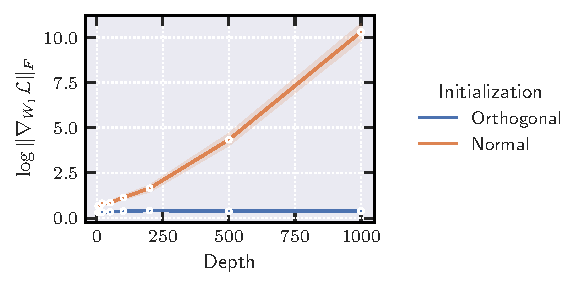
\includegraphics[width=0.75\textwidth]{figures/log_intro_figure_grad.pdf}
    \caption{Logarithmic plot for the gradient norm of the first layer for networks with different number of layers evaluated on CIFAR10. For Gaussian weights (orange) the gradient-norm grows at an exponential rate, as predicted by \citet[Theorem 3.9]{yang2018a}, while for orthogonal weights (blue) gradients remain bounded by a constant, validating Theorem~\ref{grad:thm:no_explosion}. Traces are averaged over $10$ runs and shaded regions denote the $95\%$ confidence intervals.}
    \label{grad:fig:linear_contrast_grad} 
\end{figure}

% Figure~\ref{grad:fig:linear_contrast_grad} shows that log-norms of the gradients do not explode in depth, thus validating Theorem~\ref{grad:thm:no_explosion}. In contrast, we observe in this figure that when using Gaussian weights, the gradients grow exponentially in depth, which is consistent with \citet[Theorem 3.9]{yang2018a}. 

Note that the bound is stated for the expected value of log-norm of the gradients, which can be interpreted as bits of precision needed to store the gradient matrices. Thus, the fact that depth does not appear in any form in the upper bound of Theorem~\ref{grad:thm:no_explosion} points out that training arbitrarily deep MLPs with orthogonal weights will not face numerical issues that arise with Gaussian weights~\cite{yang2018a} as long as the inputs are non-degenerate. Such guarantees are necessary to ensure backpropagation will not face numerical issues.  

 Theorem~\ref{grad:thm:no_explosion} states that as long as the input samples are not linearly dependent, the gradients remain bounded for any arbitrary depth $L$. As discussed in the previous section and evidenced in Figure~\ref{grad:fig:degenerate_input}, this is necessary to avoid gradient explosion. Therefore, the upper bound provided in Theorem~\ref{grad:thm:no_explosion} is tight in terms of inputs constraints. Furthermore, as mentioned before, random batches sampled from commonly used benchmarks, such as CIFAR10, CIFAR100, MNIST, and FashionMNIST, are non-degenerate in most practical cases (see Section~\ref{grad:sec:datasets_independence} for more details). Thus, the assumptions and thereby assertions of the theorem are valid for all practical purposes.

To the best of our knowledge, Theorem~\ref{grad:thm:no_explosion} is the first non-asymptotic gradient analysis that holds for networks with batch normalization and finite width. Previous results heavily rely on mean field analyses in asymptotic regimes, where the network width tends to infinity~\citep{yang2018a}. While mean field analyses have brought many insights about the rate of gradient explosion, they are often specific to Gaussian weights. Here, we show that non-Gaussian weights can avoid gradient explosion, which has previously been considered ``unavoidable''~\citep{yang2018a}. Figure~\ref{grad:fig:linear_contrast_grad} illustrates this pronounced discrepancy.  

\textit{Proof idea of Theorem~\ref{grad:thm:no_explosion}.}
    The first important observation is that, due to the chain rule, we can bound the log-norm of the gradient of a composition of functions, by bounding the summation of the log-norms of the input-output Jacobian of each layer, plus two additional terms corresponding to the loss term and the gradient of the first layer in the chain. If we discount the effect of the first and last terms, the bulk of the analysis is dedicated to bounding the total sum of log-norms of per layer input-output Jacobian, i.e., the fully connected and batch normalization layers. The second observation is that because the weights are only rotations, their Jacobian has eigenvalues equal to $1.$ Thus, the log-norm of gradients corresponding to fully connected layers vanish. What remains is to show that for any arbitrary depth $\ell,$ the log-norm of gradients of batch normalization layers also remains bounded. The main technical novelty for proving this step is showing that the log-norm of the gradient of $\BN$ layers is upper bounded by the isometry gap of pre-normalization matrices. Thus, we can invoke the exponential decay in isometry gap stated in Theorem~\ref{grad:thm:iso_gap_decay_in_depth} to establish a bound on the log-norm of the gradient of these layers. Finally, since the decay in isometry gap is exponentially fast, the bound on the total sum of log-norm of the gradients amounts to a geometric sum that remains bounded for any arbitrary depth $\ell.$ 


    


\section{Implications on training}
\label{grad:sec:experiments}
In this section, we experimentally validate the benefits of avoiding gradient explosion and rank collapse for training.
Thus far, we have proved that our constructed neural network with BN does not suffer from gradient explosion in Theorem~\ref{grad:thm:no_explosion}, and does not have the rank collapse issue in depth via the orthogonalization property established in Theorem~\ref{grad:thm:iso_gap_decay_in_depth}. We find that the constructed MLP is therefore less prone to numerical issues that arise when training deep networks. %Since our MLP construction simultaneously avoids exploding gradients and rank collapse, it is less prone to numerical issues that arise when training deep networks. 


\begin{figure}[ht]
    \centering
 \includegraphics[width=1\linewidth]{figures/train_CIFAR10.pdf}
 \vspace{-.8cm}
    \caption{Contrasting the training accuracy of MLPs with BN and shaped sin, shaped tanh and identity activations, on the CIFAR10 dataset. The identity activation performs much worse than the nonlinearities, confirming that the $\sin$ and $\tanh$ networks are not operating in the linear regime. The networks are trained with vanilla SGD and the hyperparameters are width $100$, batch size $100$, learning rate $0.001$.}
    \vspace{-0.3cm}
    \label{grad:fig:train_cifar10}
\end{figure}


By avoiding gradient explosion and rank collapse in depth, we observe that the optimization with vanilla minibatch Stochastic Gradient Descent (SGD) exhibits an almost depth-independent convergence rate for linear MLPs. In other words, the number of iterations to get to a certain accuracy does not vary widely between networks with different depths. Figure~\ref{grad:fig:train_cifar10} (c) shows the convergence of SGD for CIFAR10, with learning rate $0.001$, for MLPs with width $d=100$ and batch size $n=100.$ While the SGD trajectory strongly diverges from the initial conditions that we analyze theoretically, Figure~\ref{grad:fig:train_cifar10} shows that the gradients remain stable during training, as well as the fact that different depths exhibit largely similar accuracy curves. 




While the empirical evidence for our MLP with linear activation is encouraging, non-linear activations are essential parts of feature learning~\cite{nair2010rectified,klambauer2017self,hendrycks2016gaussian,maas2013rectifier}. However, introducing non-linearity violates one of the key parts of our theory, in that it prevents representations from reaching perfect isometry (see Figure~\ref{grad:fig:nonlinear_contrast} for details on the connection between non-linearities and gradient explosion in depth). Intuitively, this is due to the fact that non-linear layers, as opposed to rotations and batch normalization, perturb the isometry of representations and prevent them from reaching zero isometry gap in depth. This problem turns out to be not just a theoretical nuisance, but to play a direct role in the gradient explosion behavior.
% Figure~\ref{grad:fig:nonlinear_contrast} shows the gradient norms  explode at a fixed multiplicative rate after the isometry gap stabilizes. This means that the MLPs with non-linear activations are not able to avoid gradient explosion, in contrast to the linear case. 
While the situation may seem futile at first, it turns out that activation shaping~\citep{li2022neural,zhang2022deep,martens2021rapid,he2023deep,noci2023shaped} can alleviate this problem, which is discussed next. For the remainder of this section, we focus on the training of MLPs with non-linear activations, as well as standard batch normalization and fully connected layers.

\section{Activation shaping based on the theoretical analysis} 
In recent years, several works have attempted to overcome the challenges of training very deep networks by parameterizing activation functions. 
In a seminal work, ~\citet{martens2021rapid} propose \textit{deep kernel shaping}, which is aimed at facilitating the training of deep networks without relying on skip connections or normalization layers, and was later extended to LeakyReLU in \textit{tailored activation transformations}~\citep{zhang2022deep}. In a similar direction, ~\citet{li2022neural} propose \textit{activation shaping} in order to avoid a degenerate output covariance. While the mechanism proposed by~\citet{li2022neural} covers both smooth and non-smooth activations, we focus on their result for LeakyReLU, which consists of shaping the negative slope of the activation towards identity to ensure that the output covariance matrix remains non-degenerate when the networks becomes very deep. 

Since kernel and activation shaping aim to replace normalization, they have not been used in conjunction with normalization layers. 
In fact, in networks with batch normalization, even linear activations have non-degenerate outputs~\citep{daneshmand2021batch,yang2018a} and exploding gradients~\citep{yang2018a}. Thus, shaping activations towards identity in the presence of normalization layers may seem fruitless. Remarkably, we empirically demonstrate that we can leverage activation shaping to avoid gradient explosion in depth by using a pre-activation gain at each layer. 

% \citet{yang2018a} conclude that in the presence of batch normalization, linear activations suffer from the smallest rate of gradient explosion. However, even linear activations exhibit exponential gradient explosion in the number of layers. In comparison, our activation shaping scheme achieves a constant gradient norm in depth. This contrast can be attributed to using orthogonal weight matrices, as well as a careful activation shaping mechanism. 

\begin{figure}[ht] 
  \centering
  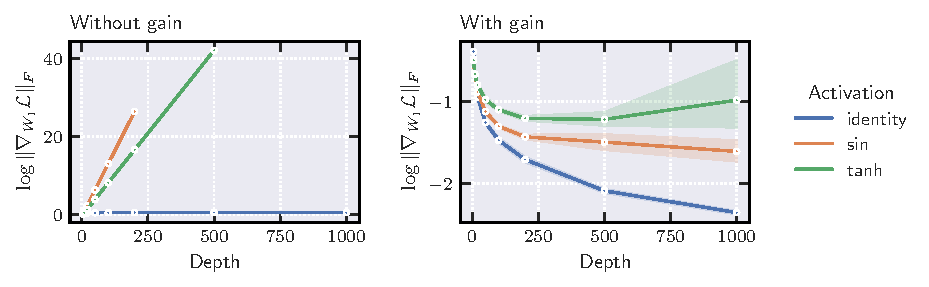
\includegraphics[width=0.8\linewidth]{figures/log_gain_vs_no_gain.pdf}
  \vspace{-.2cm}
  \caption{Logarithmic plot contrasting the effect of gain on the gradient at initialization of the first layer, for networks with different number of layers initialized with orthogonal weights, BN and different activations, evaluated on CIFAR10. The networks have hyperparameters width $100$, batch size $100$. Traces are averaged over $10$ independent runs, with the shades showing the $95\%$ confidence interval.}
  \label{grad:fig:gain_effect}
\end{figure}
Inspired by our theory, we develop a novel activation shaping scheme for networks with BN. The main strategy consists of shaping the activation function towards a linear function across the layers. Our activation shaping consists of tuning the gain of the activation, i.e., tuning $\alpha$ for $\sigma(\alpha x).$ We consider non-linear activations $\sigma \in \{\tanh, \sin\}.$  


The special property that both $\tanh$ and $\sin$ activations have in common is that they are centered, $\act(0)=0,$ are differentiable around the origin $\act'(0)=1,$ and have bounded gradients $\act'(x) \leq 1, \forall x$. Therefore, by tuning the per-layer pre-activation gain $\alpha_\ell$ towards $0$, the non-linearities behave akin to the identity function. This observation inspires us to study the relationship between the rate of gradient explosion for each layer as a function of the gain parameter $\alpha_\ell$. Formally, we consider an MLP with shaped activations using gain $\alpha_\ell$ for the $\ell$th layer, that has the update rule
\begin{align}
    X_{\ell + 1} = \act(\alpha_\ell \BN(W_\ell X_\ell))~.
    \label{grad:eqn:mlp_nonlinear}
\end{align}

% \begin{figure}[t]
%     \centering
%  \includegraphics[width=1\linewidth]{figures/plots/accuracy_plots/train_CIFAR10.pdf}
%  \vspace{-.8cm}
%     \caption{Contrasting the training accuracy of MLPs with BN and shaped sin, tanh, and identity activations on CIFAR10. The identity activation performs much worse than the nonlinearities, indicating the fact that the sin and tanh networks are not operating in the linear regime. The networks are trained with vanilla SGD and the hyperparameters are width $100$, batch size $100$, learning rate $0.001$.}
%     \label{grad:fig:train_cifar10}
% \end{figure}



Since the gradient norm has an exponential growth in depth, as shown in Figure~\ref{grad:fig:gain_effect}, we can compute the slope of the linear growth rate of log-norm of gradients in depth. We define the rate of explosion for a model of depth $L$ and gain $\alpha_\ell$ at layer $\ell$ as the slope of the log norm of the gradients $R(\ell, \alpha_\ell)$. We show in Figure~\ref{grad:fig:gain_effect} that by tuning the gain properly, we are able to reduce the exponential rate of the log-norm of the gradients by diminishing the slope of the rate curve and achieve networks trainable at arbitrary depths, while still maintaining the benefits of the non-linear activation. The main idea for our activation shaping strategy is to have a bounded total sum of rates across layers, by ensuring faster decay than a harmonic series (see App.~\ref{grad:sec:shaping} for more details on activation shaping). Figure~\ref{grad:fig:gain_effect} illustrates that this activation shaping strategy effectively avoids gradient explosion while maintaining the signal propagation and orthogonality of the outputs in depth. Furthermore, Figure~\ref{grad:fig:train_cifar10} shows that the training accuracy remains largely depth-independent. For further experiments using activation shaping, see Section~\ref{grad:sec:other_experiments}.



\section{Discussion}


\paragraph{Implicit bias of SGD towards orthogonality in optimization.} 
\begin{figure}[ht]
    \centering
    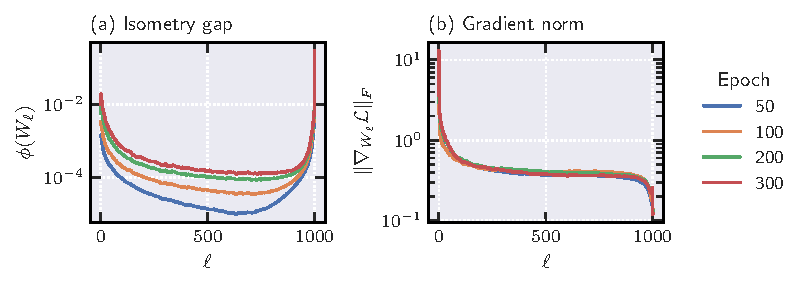
\includegraphics[width=0.9\linewidth]{figures/weight_grads_during_training_1000.pdf}
    \vspace{-.5cm}
    \caption{\textbf{Implicit orthogonality bias of SGD.} Training an MLP with width $d=100,$ batch size $n=100,$ and depth $L=1000,$ activation $\tanh$, using SGD with $\text{lr}=0.001$ (a) Isometry gap (y-axis; log-scale) of weight matrices across all layers throughout training. (b) Gradient norms at each layer during training. }
    \label{grad:fig:ortho_during_training_1000}    
\end{figure}
Optimization over orthogonal matrices has been an effective approach for training deep neural networks. Enforcing orthogonality during training ensures that the spectrum of the weight matrices remains bounded, which prevents gradient vanishing and explosion in depth. \citet{vorontsov2017orthogonality} study how different orthogonality constraints affect training performance in RNNs. For example \citet{lezcano2019cheap} leverage the exponential map on the orthogonal group, \citet{jose2018kronecker} decompose RNN transition matrices in Kronecker factors and impose soft constraints on each factor and \citet{mhammedi2017efficient} introduce a constraint based on Householder matrices.


While these studies \emph{enforce} orthogonality constraints, one of our most striking empirical observations is that when our MLP grows very deep, the middle layers remain almost orthogonal even after many steps of SGD. As shown in Figure~\ref{grad:fig:ortho_during_training_1000}, for $1000$ layer networks, the middle layers remain orthogonal during training. One could hypothesize that this is due to small gradients in these layers. In Figure~\ref{grad:fig:ortho_during_training_1000}, we observe that the gradients of these middle layers are not negligible. Thus, in our MLP construction, both with linear activation and with activation shaping, the gradient dynamics have an \emph{implicit bias} to optimize over the space of orthogonal matrices. The mechanisms underlying this implicit orthogonality bias will be an ample direction for future research.




% !TEX root = ../thesis-index.tex

%%%%%%%%%%%%%%%%%%%%%%%%%%%%%%%%%%%%%%%%%%%%%%%%%%%%%%%%%%%%%%%%%%%%%%%%%%%%%%%%
% CONCLUSION
%%%%%%%%%%%%%%%%%%%%%%%%%%%%%%%%%%%%%%%%%%%%%%%%%%%%%%%%%%%%%%%%%%%%%%%%%%%%%%%%

\chapter{Discussion and Conclusion}\label{ch:conclusion}

This thesis has made significant contributions to advancing the theoretical understanding of deep neural networks, with a particular focus on the behavior of MLPs at initialization. Despite neural networks' complex and non-linear nature, the research presented here offers several key insights into their mathematical properties. These contributions enhance the growing body of research to establish a solid theoretical foundation for deep neural networks. 

\paragraph{Contributions.}
One of the primary contributions of this work is the demonstration that BN induces orthogonality in deeply hidden representations within mini-batches. This result was elaborated in Chapter \ref{ch:bn_ortho}. Additionally, this thesis has shown that when BN is applied, the mean field approximation provides a reliable predictor of behavior even in finite-width networks, as detailed in Chapter \ref{ch:bn_MF}. Another significant finding is the layer and batch normalization tendency to bias activations toward a more isometric distribution, as discussed in Chapter \ref{ch:isometry_normalization}. Furthermore, non-linear activations promote isometry in activations, explored in Chapter \ref{ch:isometry_activation}. Finally, the work demonstrates that the problem of gradient explosion, often encountered in networks utilizing BN, can be effectively mitigated through orthogonal weight initialization, as shown in Chapter \ref{ch:bn_grad}.

From a mathematical perspective, this thesis provided two significant theoretical insights. First, we identified emergent behaviors in matrix products that arise from fully connected and normalization layers, including an intriguing property of normalization layers in Chapter~\ref{ch:isometry_normalization}. This property of normalization layers was later used in Chapter~\ref{ch:bn_grad} to analyze gradients. Second, the application of Hermite polynomials in Chapter~\ref{ch:isometry_activation} proved instrumental in shedding light on the effects of non-linear activations on signal propagation. This novel application of Hermite polynomials deepens our understanding of how non-linearity impacts signal propagation.


\paragraph{Limiations of this thesis.}
A core challenge throughout this work has been to develop a theory that is both mathematically rigorous and closely aligned with realistic neural network configurations. To achieve tractability, we made several simplifications, such as focusing on linear activations in Chapters \ref{ch:bn_ortho} and \ref{ch:bn_grad}, employing mixing-type assumptions in Chapters \ref{ch:bn_ortho} and \ref{ch:bn_MF}, assuming that batch size and network width are of the same order in Chapter \ref{ch:bn_grad}, and using mean field approximations in Chapters \ref{ch:bn_MF} and \ref{ch:isometry_activation}. Finally, the primary limitation of this dissertation is its focus on the behavior of networks at initialization with randomly chosen weights. While this assumption was critical to the tractability of the analysis, it naturally restricts the direct applicability of the results to trained networks. Extending theoretical insights to trained networks will require developing new analytical tools and methods.

Despite these necessary simplifications, the theoretical results presented here align well with observed behavior in more realistic settings where such assumptions are relaxed. This demonstrates that theoretical insights can retain practical relevance, even when derived under simplifying conditions. At the same time, the research points to certain limitations, which will be discussed in the following section.


\paragraph{Future avenues for research}
Looking ahead, several avenues of research offer promising opportunities for further exploration.   

% gradients analysis 
Analyzing training dynamics in a deep network with non-linear dynamics remains theoretically challenging. However, analyzing gradients at initialization can move us one step closer to that goal. For example, analyzing the backward gradients, particularly in terms of non-linear activations, can be highly rewarding and impactful. In particular, if we combine insights from forward and backward passes of neural networks, we can arrive at a quantitative characterization of the neural target kernel for a particular choice of activation function. 

% architectures 
One of the most important future directions involves extending the findings of this thesis to other network architectures, such as transformers and recurrent neural networks. For example, given that feedforward layers are one of the main components of transformer architecture, the insights developed in this thesis for feedforward settings can be insightful for studying how layer normalization and non-linear activation functions behave in transformers. As another example, the problem of learning long-range dependencies in recurrent settings can be viewed as a vanishing gradient problem. As we argued in several chapters, batch normalization is an effective module for dealing with vanishing gradients in a feedforward setup. While these insights are not directly applicable to recurrent settings, finding analogs of batch normalization in a recurrent setting is worth exploring. Alternatively, insights on the importance of initialization in Chapter~\ref{ch:bn_grad} and Chapter~\ref{ch:bn_ortho} can provide new perspectives on leveraging initialization to control gradients in recurrent architectures.


% non mean field 
As mentioned earlier in limitations, the mean field assumption that the width of the network tends to infinity was a necessary simplification in some of our theoretical analyses. While this assumption has considerable benefits, it also raises questions as to the accuracy of the theoretical predictions. While we saw in Chapter~\ref{ch:bn_MF} that in some cases, these predictions are accurate, developing non-asymptotic results remains a significant theoretical challenge. A middle-ground approach that has shown promise and higher accuracy is tending the width and depth of the network to infinity while keeping their ratio constant. 


% free probability 

\paragraph{Concluding remarks.}
In conclusion, this dissertation advances our mathematical understanding of deep neural networks, particularly in signal propagation, normalization techniques, and initialization strategies. By applying a fresh mathematical perspective, this work has laid the groundwork for future research to bridge the gap between theoretical understanding and practical application in deep learning. 
The need for robust theoretical foundations becomes increasingly critical as neural networks grow in complexity and capability. This work contributes to that foundation, offering both immediate insights and promising avenues for future exploration in theory of neural networks. 

\cleardoublepageempty{}

%%%%%%%%%%%%%%%%%%%%%%%%%%%%%%%%%%%%%%%%
% APPENDIX %
%%%%%%%%%%%%%%%%%%%%%%%%%%%%%%%%%%%%%%%%
\appendix
% \part{Appendix}


\chapter{Detailed proofs of Chapter~\ref{ch:bn_ortho}}


 \section{Preliminaries}
%  \subsection*{Notations}
 Let $v,w \in \R^{k}$ then $v \odot w \in \R^{n}$ with coordinates
 \begin{align}
     [v \odot w ]_{i} = v_i w_i
 \end{align}
 Furthermore $v^{\otimes 2} \in \R^{k \times k}$ with entities
 \begin{align}
     [v^{\otimes 2}]_{ij} = v_i v_j. 
 \end{align}
 In Table~\ref{ortho:tab:notations}, we summarize notations introduced previously. 
 \begin{table}[!ht]
     \centering
     \begin{tabular}{|l|l l|}
     \hline
        Notation & Type & Definition \\ 
        \hline
        $\ell$  & integer & number of layers\\
        $n$  & integer & batch size \\ 
        $d$ & integer & width of the network\\ 
        $k$ & integer & output dimension \\ 
        $X$ & $\R^{d\times n}$ & input matrix\\ 
        $H_\ell$ & $\R^{d\times n}$ & hidden representations at $\ell$ (obeying Eq.~\eqref{ortho:eq:bn_recurrence})\\
        $BN$ & $\R^{d\times n} \to \R^{d\times n}$ & batch normalization layer (defined in Eq.\eqref{ortho:eq:bn_recurrence}) \\ 
        $\text{Law}(X)$ &  & the law of random matrix $X$ \\ 
        $\sigma_i(M)$ & $\R^{k_1\times k_2} \to \R_+$ & the $i$th largest singular value of matrix $M$ \\ 
        $I_k$ & $\R^{k \times k}$ & Identity matrix of size $k$ \\
        $\ones_k$ & $\R^n$ &  all-ones vector
       \\ \hline
     \end{tabular}
     \vspace{0.1cm}
    \caption{Summary of notations used in this chapter.}
     \label{ortho:tab:notations}
 \end{table}
 \subsection*{The Markov chain of hidden representations} Recall the chain of the hidden representations, denoted by $\{ H_\ell\in \R^{d\times n} \}$, obeying the following recurrence: 
 \begin{align} \label{ortho:eq:BNrecurrence_app}
     H_{\ell+1} = \frac{1}{\sqrt{d}}
     BN(W_\ell H_\ell), \quad BN(M) = \left(\diag(M M^\top)\right)^{-\sfrac{1}{2}}M,
 \end{align}
 where $W_\ell \in \R^{d\times n}$ are random weight matrices with i.i.d. zero-mean Gaussian elements. It is easy to check that the Frobenius norm of $H_\ell$ is one due to the row-wise normalization: 
 \begin{equation}
  \label{ortho:eq:unitnorm_app}   
 \begin{aligned} 
    \tr \left(  BN(H) BN(H)^\top \right) & = \tr\left( \diag(H H^\top)^{-\sfrac{1}{2}} H H^\top\diag(H H^\top)^{-\sfrac{1}{2}}\right) \\ 
    & = \tr\left( \diag(H H^\top)^{-1} H H^\top\right) \\ 
    & = d.
 \end{aligned}
 \end{equation}
 \subsection*{Lyapunov function characterizing the orthogonality}
 We introduce the following function serving as a Lyapunov function $\widehat{V}:\R^{d\times n}$ characterizing the orthogonality of the hidden representations:
 \begin{align}
     \widehat{V}(H) = \frac{1}{n} - (\sigma_n (H))^2,
 \end{align}
 where $\sigma_n(H)$ is the minimum singular value of matrix $H$. Next lemma proves $\widehat{V}(H_\ell)$ bounds the orthogonality gap. 
 \begin{lemma} \label{ortho:lemma:Vbound}
 For all hidden representations $H_\ell$, the following holds:
 \begin{align}
     V(H_\ell) \leq 2 n \widehat{V}(H_\ell) \nonumber. 
 \end{align}
 \end{lemma}
 \begin{proof}
 Let $\sigma_1, \dots, \sigma_n$ be the singular values of $H_\ell$. Given these singular values, one can compute $V(H_\ell)$ as 
 \begin{align*}
     (V(H_\ell))^2 = \sum_{i=1}^n \left(\sigma_i^2-\frac{1}{n}\right)^2 \nonumber.
 \end{align*}
 According to Eq.~\eqref{ortho:eq:unitnorm_app}, $\sum_{i=1}^2 \sigma_i^2 = 1$ holds. The proof is an immediate consequence of this propery.   
 \begin{align} \nonumber
     V^2(H_\ell) &=  \sum_{i=1}^n \sigma_i^4 - 2 \underbrace{\left(\sum_{i=1}^n \sigma_i^2  \right)}_{=1}\frac{1}{n} + \frac{1}{n}\\ 
     & = \sum_{i=1}^n \sigma_i^4 -\frac{1}{n}. \nonumber
 \end{align}
 For a freeze $\sigma_n$, the maximum of $\sum_{i=1}^n \sigma_i^4 -\frac{1}{n}$ subject to $\sum_{i=1}^n \sigma_i^2 = 1$ is met when $\sigma_1^2 = 1-(n-1)\sigma_n^2$ and $\sigma_2 = \dots = \sigma_n$.
 Using this optimal values, we get the following bound:
 \begin{align} \nonumber
     V^2(H_\ell) \leq 2(n-1)^2 \underbrace{\left( \frac{1}{n} - \sigma_n^2\right)^2}_{=\widehat{V}^2(H_\ell(X))}.
 \end{align}
 Taking the square root of both sides concludes the proof.
 \end{proof}
 
 
 
 \section{Proof of Theorem~\ref{ortho:thm:contraction}}
 
 The proof of Theorem~\ref{ortho:thm:contraction} relies on the following Theorem that characterizes the change of $\widehat{V}$ in consecutive layers. 
 \begin{theorem} \label{ortho:thm:single_update}
 The sequence $\{ H_\ell \}$ obeys
 \begin{align*}
  \E \left[ \widehat{V}(H_{\ell+1}) | H_\ell \right] \leq \left(1- \frac{2}{3} \left(\frac{1}{n}- \widehat{V}(H_\ell)\right) \right) \widehat{V}(H_\ell) + \frac{1}{\sqrt{d}}.
 \end{align*}
 \end{theorem}
 Notably, the above result does not rely on Assumption \ref{ortho:assume:lineary_indepdence}.  Assuming that  Assumption \ref{ortho:assume:lineary_indepdence} holds, we complete the proof of Theorem~\ref{ortho:thm:contraction}. Combining the last Theorem by this assumption, we get 
 \begin{align} \label{ortho:eq:lyp_condition}
     \E \left[ \widehat{V}(H_{\ell+1}) \right] \leq \left(1-\frac{2}{3}\alpha\right) \E \left[ 
 \widehat{V}(H_\ell)\right] + \frac{1}{\sqrt{d}} 
 \end{align}
 Induction over $\ell$ yields
 \begin{align*}
     \E \left[ \widehat{V}(H_{\ell+1}(X)) \right] & \leq  \left(1-\frac{2}{3}\alpha\right)^{\ell} \E \left[ 
 \widehat{V}(H_1)\right] + \left(\sum_{k=1}^\ell (1-\frac{2}{3}\alpha)^k\right)\frac{1}{\sqrt{d}} \\
     & \leq \left(1-\frac{2}{3}\alpha\right)^{\ell} \E \left[ 
 \widehat{V}(H_1)\right] + \frac{3}{2\alpha\sqrt{d}} 
 \end{align*}
 An application of Lemma~\ref{ortho:lemma:Vbound} completes the proof: 
 \begin{align*}
     \E \left[ V(H_{\ell+1}) \right] & \leq 2 n \E \left[ \widehat{V}(H_{\ell+1}) \right] \\ 
     & \leq 2 \left(1-\frac{2}{3}\alpha\right)^{\ell}+ \frac{3 n}{2 \alpha\sqrt{d}} 
 \end{align*}
 \subsection*{Stability analysis without technical assumption}
 Using Theorem~\ref{ortho:thm:single_update}, we can prove stability of the chain $\{ H_\ell \}$ without Assumption~\ref{ortho:assume:lineary_indepdence}. After rearrangement of terms in Theorem~\ref{ortho:thm:single_update}, we get
 \begin{align*}
     \E \left[ \widehat{V}(H_{\ell+1})| H_\ell \right] - \widehat{V}(H_\ell) \leq - \frac{2}{3} \widehat{V}(H_\ell) \left( \frac{1}{n}- \widehat{V}(H_\ell) \right) + \frac{1}{ \sqrt{d}}
 \end{align*}
 Taking the expectation over $H_\ell$ and average over $\ell$ yields
 \begin{align*}
     \E \left[\frac{1}{\ell}\sum_{k=1}^\ell \widehat{V}(H_k) \left( \frac{1}{n}- \widehat{V}(H_k)\right)\right]  \leq \left(\frac{3 \E \left[ \widehat{V}(H_0) \right]}{2 \ell}\right) +\frac{3}{2 \sqrt{d}}
 \end{align*}
 
 
 \section{Proof of Theorem~\ref{ortho:thm:single_update}}
 \label{ortho:sec:proof_thm}
  
 \subsection*{Spectral decomposition.}
 Consider the SVD decomposition of $H_{\ell}$ as $H_{\ell} = U \diag(\sigma) V^\top$ where $U$ and $V$ are orthogonal matrices. Given this decomposition, we get
 \begin{align} \label{ortho:eq:wh}
     W_{\ell} H_{\ell} = \underbrace{W_{\ell} U}_{W} \diag(\sigma) V^\top 
 \end{align}
 Since $W_{\ell}$ is Gaussian and $U$ is an orthogonal matrix, entities of $W$ are also i.i.d. standard normal. We will repeatedly use the above decomposition in our analyses.
 
 
 \subsection*{Concentration analysis.}
 Consider matrix $C_{\ell+1} := H_{\ell+1}^\top H_{\ell+1}$ whose eigenvalues are $\sigma_1^2, \dots, \sigma_n^2$. The SVD decomposition of $H_\ell$ in Eq.~\eqref{ortho:eq:wh} allows us to write $C_{\ell+1}$ as 
 \begin{align*}
     C_{\ell+1} = \frac{1}{d}\sum_{i=1}^d \left( \frac{w_i \odot \sigma }{\| w_i \odot \sigma \|_2 } \right)^{\otimes 2}
 \end{align*}
 where $w_i \in \R^n$ is the $i$-th row of $W$, and $\sigma \in \R^n$ is the vector of singular values of $H_\ell$. Thus, conditioned on $\sigma$, $C_{\ell+1}$ is an empirical average of i.i.d. random vectors. This allows us to prove that this empirical average is concentrated around its expected value. The next lemma states this concentration. 
 \begin{lemma} \label{ortho:lemma:cov_concentration} 
 The following concentration always holds
 \begin{align*}
      \E_{W_{\ell}} \| C_{\ell+1} - \E_{W_\ell} \left[ C_{\ell+1}
     \right] \|^2 \leq 1/d  
 \end{align*}
 where 
 \begin{align} \label{ortho:eq:pn}
     \E_{W_\ell} \left[ C_{\ell+1}
     \right] = \diag(p_1(\sigma), \dots, p_n(\sigma)), \quad p_i(\sigma) := \E \left[ \frac{\sigma_n^2 w_n^2}{\sum_{k=1}^n \sigma_k^2 w_k^2} \right], \quad w_{i} \stackrel{\text{i.i.d.}}{\sim} \N(0,1)
 \end{align}
 \end{lemma}
 The concentration of $C_{\ell+1}$ allows us to prove that the Lyapunov function $\widehat{V}(H_{\ell+1})$ is concentrated around $1/n-p_n(\sigma)$. 
 \begin{lemma}
 The following holds 
 \label{ortho:lemma:concentration}
 \begin{align*}
  \E_{W_{\ell}} \left[ \left( \widehat{V}(H_{\ell+1}) - (1/n-p_n(\sigma))  \right)^2 \right] \leq \frac{1}{d}
  \end{align*}.
 \end{lemma}
 The last lemma allows us to predict the value of random variable $\widehat{V}(H_{\ell+1})$ by deterministic term $1/n-p_n(\sigma)$. 
 \subsubsection*{Contraction.} 
 The decay in $\widehat{V}(H_{\ell+1})$ with $\ell$ is due to term $1/n-p_n(\sigma)$ in the last lemma. This term is less than (or equal to) $V(H_\ell)$.
 \begin{lemma} \label{ortho:lemma:concentration_center}
 For $p_n(\sigma)$ defined in Eq.~\eqref{ortho:eq:pn}, the following holds:
 \begin{align*}
   \left( \frac{1}{n}- p_n(\sigma) \right) \leq \left(1- \frac{2}{3} \left(\frac{1}{n}- \widehat{V}(H_\ell)\right) \right) \widehat{V}(H_\ell).
 \end{align*}
 \end{lemma}
 Combining the last lemma by Lemma~\ref{ortho:lemma:concentration} concludes the proof of Theorem~\ref{ortho:thm:single_update}: 
 \begin{align} \label{ortho:eq:onestep_result_app}
     \E_{W_\ell} \left[  \widehat{V}(H_{\ell+1}) \right] \leq  \left(1- \frac{2}{3} \left(\frac{1}{n}- \widehat{V}(H_\ell)\right) \right) \widehat{V}(H_\ell) + \frac{1}{\sqrt{d}}.
   \end{align}
 To complete the proof, we prove Lemmas~\ref{ortho:lemma:cov_concentration}, \ref{ortho:lemma:concentration}, and \ref{ortho:lemma:concentration_center}.
 \subsubsection*{Proof of Lemma~\ref{ortho:lemma:cov_concentration}}
 Given the spectral decomposition of $H_{\ell}$ in Eq.~\eqref{ortho:eq:wh}, we compute element $ij$ of $C_{\ell+1}$, which is denoted by $[C_{\ell+1}]_{ij}$:
 \begin{align*}
      [C_{\ell+1}]_{ij} = [A^\top A]_{ij} = \frac{1}{d} \sum_{k=1}^d A_{ki} A_{kj}, \quad A_{ki} = W_{ki} \sigma_i/\sqrt{v_k}
 \end{align*}
 where $v_k = \sum_{m=1}^n W_{km}^2 \sigma_m^2 $. Since $W_{km}$ are zero mean and unit variace, we get
 \begin{align*}
    \E [C_{\ell+1}]_{ij} & = 0 \\
    \E [C_{\ell+1}]_{ij}^2 & = \frac{1}{d^2}\sum_{k=1}^d A_{ki}^2 A_{kj}^2 +  \frac{1}{d^2}\sum_{k,k'}^d \underbrace{\E \left[ A_{ki}^2 A_{kj}^2  A_{k'i}^2 A_{k'j}^2\right]}_{=0} \\ 
    & = \frac{1}{d^2}\sum_{k=1}^d A_{ki}^2 A_{kj}^2 
 \end{align*}
 holds for $i\neq j$.
 By summing up over $i \neq j$, we get 
 \begin{align*}
     \sum_{i \neq j} \E [C_{\ell+1}]_{ij} = \frac{1}{d^2} \left(\sum_{k} \left( \sum_{i} A_{ki}^2 \right)^2 - \sum_{ik} A_{ki}^4\right)
 \end{align*}
 For the diagonal elements, we get 
 \begin{align*}
     \E \left[ C_{\ell+1} \right]_{ii} & = \frac{1}{d}\sum_{k=1}^d \E A_{ki}^2 \\ 
     & = \frac{1}{d}\sum_{k=1}^d \E A_{ki}^2 \\ 
     & = \underbrace{\frac{1}{d}\sum_{k=1}^d \E \left[ \frac{W_{ki}^2 \sigma_i^2 }{\sum_{j=1}^n W_{kj}^2 \sigma_j^2} \right]}_{p_i(\sigma)}
 \end{align*}
 The variance of $[C_{\ell+1}]_{ii}$ is bounded as 
 \begin{align*}
      \text{var}([C_{\ell+1}]_{ii}) & = \E \left(\frac{1}{d}\sum_{k=1}^d (A_{ki}^2 - p_i(\sigma))\right)^2 \\ 
      & = \frac{1}{d^2}\sum_{k=1}^d (A_{ki}^2 - p_i(\sigma))^2 \\
      & \leq \frac{1}{d^2}\sum_{k=1}^d A_{ki}^4 
 \end{align*}
 Combining results for the diagonal and off-diagonal elements yields
 \begin{align*}
     \E \| C_{\ell+1} - \E_{W_{\ell}} \left[ C_{\ell+1} \right] \|_F^2 & = \sum_{ij} \text{var}([C_{\ell+1}]_{ij}) \\
     & \leq  \frac{1}{d^2} \left( \sum_{i} A_{ki}^2 \right)^2 =1/d
 \end{align*}
 \subsection*{Proof of Lemma~\ref{ortho:lemma:concentration}}
 Notably, the eigenvalues of $C_{\ell+1}$ are squared singular values of $H_{\ell+1}$. Let $\lambda_n(C)$ denote the $n$th largest eigenvalue of matrix $C$. 
 \begin{align*}
     \E_{W_{\ell}} \left[ \left( \widehat{V}(C_{\ell+1}) - \left(\frac{1}{n} - p_n(\sigma)\right) \right)^2 \right] & \leq \E_{W_{\ell}} \left[ \left(\lambda_n\left(C_{\ell+1}\right) - \lambda_n\left(\E_{W_{\ell}} \left[ C_{\ell+1} \right]\right) \right)^2\right] \\ 
     & = \E_{W_\ell} \left[ \| C_{\ell+1} - \E_{W_{\ell}} \left[ C_{\ell+1} \right] \|_F^2  \right] \\ 
     & \leq \frac{1}{d}
 \end{align*}
 where the last inequality relies on Lemma~\ref{ortho:lemma:cov_concentration}. 
 \subsubsection*{Proof of Lemma~\ref{ortho:lemma:concentration_center}}
 The proof is based an application of moment generating function that allows us to compute expectations of ratios of random variables. 
 \begin{lemma}[Lemma~1 in ~\citep{sawa1972finite}]
 Let $X_1$ be a random variable that is positive with probability one and $X_2$  be an arbitrary random variable. Suppose that there exists a joint moment generating function of $X_1$ and $X_2$: 
 \begin{align*}
     \phi(\theta_1,\theta_2) = \E \left[ \exp(\theta_1 X_1 + \theta_2 X_2) \right]
 \end{align*}
 for $ \theta_1 \leq \epsilon$ and $| \theta_2 | <\epsilon$ where $\epsilon$ is some positive constant. Then 
 \begin{align*}
     \E \left[ \frac{X_2}{X_1}\right] = \int_{-\infty}^0 \left[\frac{\partial \phi(\theta_1,\theta_2)}{\partial \theta_2} \right]_{\theta_2 = 0 } d \theta_1 
 \end{align*}
 \end{lemma}
 \noindent To estimate $p_n(\sigma)$, we set $X_2 := \sigma_i^2 w_i^2$ and $X_1 = \sum_{j} \sigma_j^2 w_j^2 $, which obtains 
 \begin{align*}
     \phi&(\theta_1,\theta_2) \\
     & = \E \left[ \exp(\theta_1 X_1 + \theta_2 X_2) \right] \nonumber\\ 
     & = (2\pi)^{-n/2}\int_{-\infty}^{\infty}\exp( (\theta_1 + \theta_2) \sigma_i^2 w_i^2 + \sum_{j\neq i} \theta_1 \sigma_j^2 w_j^2) \exp(-\sum_{k} w_k^2/2) d w \\ 
     & = (2\pi)^{-n/2}\int_{-\infty}^{\infty} \exp(\left(-0.5+(\theta_1+\theta_2) \sigma_i^2\right) w_i^2) d w_i  \left(\prod_{j\neq i} \int_{-\infty}^{\infty} \exp(\left(-0.5+\theta_1 \sigma_j^2\right) w_j^2) d w_j\right)\\ 
     & = \frac{1}{\sqrt{1-2 (\theta_1 +  \theta_2)\sigma_i^2}} \left( \prod_{j\neq i} \frac{1}{\sqrt{1-2\theta_1 \sigma_j^2}} \right).
 \end{align*}
 Taking derivative with respect to $\theta_2$ yields 
 \begin{align*}
     \frac{\partial \phi}{\theta_2}(\theta_1,0) = \frac{\sigma_i^2}{(1-2 \theta_1\sigma_i^2)^{3/2}}\left( \prod_{j\neq i} \frac{1}{\sqrt{1-2\theta_1 \sigma_j^2}} \right)
 \end{align*}
 Using the result of the last lemma, we get 
 \begin{align*}
     p_i(\sigma) = \int_{-\infty}^0 \frac{\sigma_i^2}{(1-2 \theta\sigma_i^2)}\left( \prod_{j} \frac{1}{\sqrt{1-2\theta \sigma_j^2}} \right) d\theta
 \end{align*}
 % \paragraph{A sanity check:} It is easy to check that
 % \begin{align}
 %   \frac{\sigma_i^2}{(1-2 \theta\sigma_i^2)}\left( \prod_{j} \frac{1}{\sqrt{1-2\theta \sigma_j^2}} \right) = d\left(\prod_{j} \frac{1}{\sqrt{1-2\theta \sigma_j^2}}\right)/d\theta
 % \end{align}
 % Hence $\sum_{i=1}^p p_i(\sigma) = 1$. \\
 Therefore, 
 \begin{align} \label{ortho:eq:pnbound}
      p_n(\sigma) = \sigma_n^2 f_n(\sigma), \quad f_n(\sigma) :=  \int_{-\infty}^0 \frac{d\theta }{(1-2\theta\sigma_n^2)^{\sfrac{3}{2}}\prod_{j\neq n}(1-2\theta \sigma_j^2)^{\sfrac{1}{2}}} 
  \end{align}
 Since $\sum_{i=1}^n \sigma_i^2 = 1$ holds (see Eq.~\eqref{ortho:eq:unitnorm_app}), $f_n(\sigma)$ in the above formulation is minimized when the $\sigma_j^2$s are all equal for all $j\neq n$. Let $\sigma_n^2:=1/n-\delta$ and $\sigma_j^2:=1/n+\delta/(n-1)$ for all $j\neq i$. This allows us to establish a lowerbound on $f_n(\sigma)$ as
 \begin{align} \label{ortho:eq:g}
 f_n(\sigma) &\ge \int_0^\infty \underbrace{\left(1+2\theta\left(\frac{1}{n}-\delta\right)\right)^{-\frac{3}{2}}\left(1+2\theta\left(\frac{1}{n}+\frac{\delta}{n-1}\right)\right)^{-\frac{n-1}{2}}}_{g(\delta):=} d\theta
 \end{align}
 Next lemma proves that $g(\delta)$ is a convex function for $\delta \in [0,1/n]$. 
 \begin{lemma} \label{ortho:lemma:convexity_g}
   The function $g(\delta)$, which is defined in Eq.~\eqref{ortho:eq:g}, is a convex function on domain $\delta \in [0,1/n]$. 
 \end{lemma}
 The convexity of $g(\delta)$ yields
 \begin{align*}
 g''(\delta)\ge 0\; \forall \delta &\implies g(\delta) \ge g(0) + \delta g'(0)
 \end{align*}
 The above bound allow us to bound $f_n(\sigma)$ as 
 \begin{align*}
     f_n(\sigma)&\ge \int_0^\infty g(0)d\theta + \delta \int_0^\infty 2\theta\left(1+\frac{2\theta}{n}\right)^{-\frac{n}{2}-2} d\theta \\
  &= 1 +\frac{2  \delta n}{n+2}
 \end{align*}
 Note that we use integration by parts to compute the above integrals. 
 Recall $\delta = \frac{1}{n}- \sigma_n^2$.
 Combining the above inequality by Eq.~\eqref{ortho:eq:pnbound} concludes the proof of the Lemma~\ref{ortho:lemma:concentration_center}:
 \begin{align*}
     \frac{1}{n} - p_n(\sigma) \leq \left(1-\frac{2n}{(n+2)}\sigma_n^2\right)\left(\frac{1}{n} - \sigma_n^2\right)
 \end{align*}
 % Notably, the lower-bound is tight for $f_i(\sigma)$ as it is illustrated in the following Figure.
 %  \begin{figure}[!ht]
 %     \centering
 %      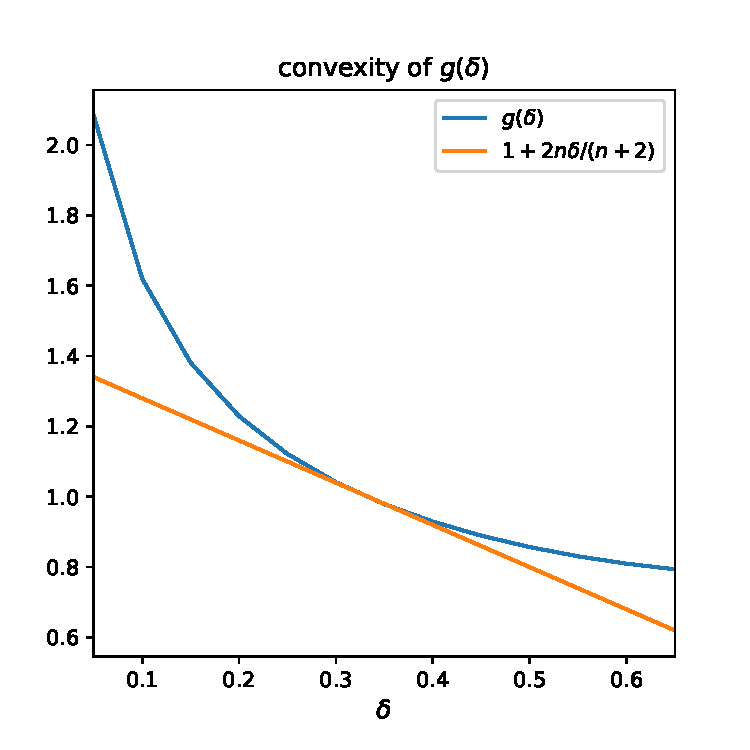
\includegraphics[width=0.4\textwidth]{figures/lemma6_convexity.pdf} 
 % \end{figure}
 \subsubsection*{Proof of Lemma~\ref{ortho:lemma:convexity_g}}
 We can show convexity of $g(\delta)$ by showing $g''(\delta)\ge 0$ for all $\delta\in [0,1/n]$. To this end, 
 we define function $h_1(\delta)$ (for the compactness of notations) as
 \begin{align*}
 h_1(\delta):=\left(1+2\theta\left(\frac{1}{n}-\delta\right)\right)^{-5/2}\left(1+2\theta\left(\frac{1}{n}+\frac{\delta}{n-1}\right)\right)^{-\frac{n-1}{2}-1}.
 \end{align*}
 Given $h_1$, the derivative of $g$ reads as 
 \begin{align*}
 % g(\delta)&:=\left(1+2\theta(\frac{1}{n}-\delta)\right)^{-3/2}\left(1+2\theta(\frac{1}{n}+\frac{\delta}{n-1})\right)\\
 g'(\delta) &=  h_1(\delta)\left( -\frac{3}{2}(-2\theta)\left(1+2\theta\left(\frac{1}{n}+\frac{\delta}{n-1}\right)\right) - \frac{n-1}{2}\left(\frac{2\theta}{n-1}\right) \left(1+2\theta\left(\frac{1}{n}-\delta\right)\right)\right)\\
 &= \theta h_1(\delta) \left(3 + \theta\frac{6}{n} + \theta\delta\frac{6}{n-1}-1-\frac{2 \theta}{n}+2\theta\delta\right)\\
 &= \theta h_1(\delta) \underbrace{\left(2+\theta \frac{4}{n}+\theta\delta\frac{2n+4}{n-1}\right)}_{h_2(\delta):=}\\
 &= \theta h_1(\delta) h_2(\delta).
 \end{align*}
 One can readily check that $h_2'(\delta) \ge 0$. Hence, $h_1'(\delta)\ge 0$ ensures the convexity of $g(\delta)$. Consider the following auxiliary function
 $$h_3(\delta):=\left(1+2\theta\left(\frac{1}{n}-\delta\right)\right)^{-7/2}\left(1+2\theta\left(\frac{1}{n}+\frac{\delta}{n-1}\right)\right)^{-\frac{n-1}{2}-2}.$$
 Given $h_3$, we compute $h'_1$ as 
 \begin{align*}
 h_1'(\delta) &= h_3(\delta)\left(\left(-\frac{5}{2}\right)\left(-2\theta\right)\left(1+2\theta\left(\frac{1}{n}+\frac{\delta}{n-1}\right)\right) + \left(-\frac{n-3}{2}\right)\frac{2\theta}{n-1}\left(1+2\theta\left(\frac{1}{n}-\delta\right)\right)\right)\\
 &= h_3(\delta)\theta\left(5(1+2\theta/n+\frac{2\theta\delta}{n-1}) - \frac{n-3}{n-1}(1+2\theta/n-2\theta\delta)\right)\\
 &=h_3(\delta)\theta\underbrace{\left(\frac{4n-2}{n-1}+2\theta\frac{4n-2}{n(n-1)}+2\theta\delta\frac{n+2}{n-1}\right)}_{h_4(\delta):=}\\
 &=\theta h_3(\delta) h_4(\delta).
 \end{align*}
 Clearly we have $h_3(\delta),h_4(\delta)\ge 0$ for $\delta \in [0,\frac{1}{n}]$. Therefore, the proof is complete.  
 
 
 % \begin{lemma} \label{ortho:lemma:distance_bound}
 %   For $H_{\ell}$ obeying Eq.~\eqref{ortho:eq:bn_recurrence}, the following holds 
 %   \begin{align}
 %       \| [\sigma_1(H_\ell), \dots, \sigma_n(H_{\ell})] - [1/\sqrt{n}, \dots, 1/\sqrt{n}] \|^2_2 \leq n^3 \left( V(H_\ell) \right)^2 
 %   \end{align}
 %  \end{lemma}
%  \subsection*{Results for vanilla networks} \label{ortho:sec:vanilla_theory}
 To compare networks with and without BN,
  next lemma formally establishes the contraction of orthogonality gap to a large value for networks withou BN. 
 \begin{lemma} \label{ortho:lemma:linear}
 Let $S_{\ell} = W_{\ell} \dots W_{1}$. Then, there exists a positive constant $\delta$ such that the following holds
 \begin{align}
       \lim_{\ell \to \infty} \frac{1}{2 \ell}\log\left( \left|V(S_\ell)-\sqrt{\frac{n-1}{n}}\right|\right) \leq -\delta. 
  \end{align}
 \end{lemma} 
 In other words, the gap $V(S_\ell)$ converges to $\sqrt{(n-1)/n}$ with asymptotic rate $\exp(-\delta \ell)$ for the identity inputs. While, Thm.~\ref{ortho:thm:contraction} proves the gap for BN networks converges to $n/\sqrt{d}$ with an exponential rate. For a sufficiently large $d$, $n/\sqrt{d} \ll \sqrt{(n-1)/n}$ holds.
 \begin{proof}
 
 Let $\sigma_1(\ell) \geq \sigma_2(\ell) \geq  \dots \geq  \sigma_n(\ell)$ denote singular values of matrix $S_\ell$, then it is known that 
  \begin{align}
      \lim_{\ell \to \infty} \frac{1}{\ell} \log(\sigma_i^2(\ell)) = \frac{1}{2} \left( \log(2) + \Psi\left(\frac{d-i+1}{2}\right) \right) 
  \end{align}
  holds where $\Psi$ is digamma function~\citep{newman1986distribution}, which a monotonically decreasing function. Therefore, 
  \begin{align} 
       \lim_{\ell \to \infty} \frac{1}{\ell} \left( \log(\sigma_2^2(\ell)) - \log(\sigma^2_1(\ell)) \right)  = - \delta <0 
  \end{align}
  holds for $\delta>0$ that can be exactly computed using function $\Psi$. The above inequality implies that $\sigma_1^2(\ell)$ increases (or decreases) faster than $\sigma_2^2(\ell)$ with an exponential rate. 
  Using this result, we get the following limit for $j\neq 1$:
  \begin{align} \label{ortho:eq:delta_bound1} 
     \lim_{\ell \to \infty} \frac{1}{\ell} \log\left(\frac{\sigma_j^2(\ell)}{\sum_{i} \sigma_i^2(\ell)}\right) \leq \lim_{\ell \to \infty} \frac{1}{\ell} \log\left(\frac{\sigma_2^2(\ell)}{ \sigma_1^2(\ell)}\right) = -\delta
  \end{align}
  Furthermore,
  \begin{align} 
  \label{ortho:eq:delta_bound2}
      \lim_{\ell \to \infty} \frac{1}{2\ell} \log\left|\frac{\sigma_1^2(\ell)}{\sum_{i} \sigma_i^2(\ell)} - 1\right| 
       \leq \lim_{\ell \to \infty} \frac{1}{\ell} \log\left|\frac{n \sigma_2^2(\ell) }{ \sigma_1^2(\ell)}\right| \leq -\delta + \lim_{\ell \to \infty} \log(n)/\ell \leq -\delta 
  \end{align}
  Let $\sigma(\ell) = (\sigma_1^2(\ell), \dots, \sigma_n^2(\ell)) \in \R^n$ and $1_n$ is the all one vector in $\R^n$ and $e_1 = (1,0, \dots, 0)\in \R^n$.
  Using triangular inequality, we get
  \begin{align}
      \left| V(S_\ell) -  \sqrt{(n-1)/n} \right| & = \left|  \left\| \frac{\sigma(\ell)}{\| \sigma(\ell)  \|_1 }- \frac{1}{n} 1_n \right\| - \left\| e_1 -  \frac{1}{n} 1_n  \right\|    \right|  \leq \left\| \frac{\sigma(\ell)}{\| \sigma(\ell)  \|_1} - e_1 \right\| 
  \end{align}
  Therefore, we get
 
   \begin{multline}
      \lim_{\ell \to \infty} \frac{1}{\ell} \log\left( \left|V(S_\ell)-\sqrt{\frac{n-1}{n}}\right|\right) \\ \leq 
      \lim_{\ell \to \infty} \left( \frac{1}{4\ell} \log \left( 2n \left(\frac{\sigma_2^2(\ell)}{\sum_{j} \sigma_j^2(\ell)} \right)  \right) + \frac{1}{4\ell} \log\left(2  \left( \frac{\sigma_1^2(\ell)}{\sum_{j} \sigma_j^2(\ell)} - 1 \right)^2 \right)\right)
   \end{multline}
  which is bounded by $-\delta$ according to the established bounds in Eq.~\eqref{ortho:eq:delta_bound1}, and Eq.~\eqref{ortho:eq:delta_bound2}. 
  \end{proof}
 
\subsection*{Proof of Lemma~\ref{ortho:lemma:wv_bound}}
 The main idea is based on a particular coupling of random matrices $W_\ell H_\ell$ and $G$. Consider the truncated SVD decomposition of $H_\ell$ as $H_\ell = U \diag(\sigma) V^\top $ where $U \in \R^{d\times n}$ and $V \in \R^{n \times n}$ are orthogonal matrices. Due to the orthogonality, the law of $W_\ell U$ is the same as those of $G V $. By coupling $W_\ell U = G V$, we get 
 \begin{equation*}
 \begin{aligned}
     \left(\mathcal{W}_2(W_\ell H_\ell, G/\sqrt{n})\right)^2 & = \inf_{\text{all the couplings}}\E \|   W_\ell U \diag(\sigma) V^\top  - GVV^\top/\sqrt{n} \|_F^2 \\ 
     & \leq \E \| GV \left( \diag(\sigma) - I/\sqrt{n} \right) V^\top \|_F^2 \\ 
     & = \E \tr(GV \left( \diag(\sigma) - I/\sqrt{n} \right) V^\top V \left( \diag(\sigma) - I/\sqrt{n} \right) V^\top G^\top ) \\ 
     & =  \tr(V \left( \diag(\sigma) - I/\sqrt{n} \right) \left( \diag(\sigma) - I/\sqrt{n} \right) V^\top \E \left[ G^\top G \right] ) \\ 
     &= \E \tr( \left( \diag(\sigma) - I/\sqrt{n} \right) \left( \diag(\sigma) - I/\sqrt{n} \right) V^\top V )  \\ 
     &= \E \| \left( \diag(\sigma) - I/\sqrt{n} \right) \|_F^2 \\
     & = \E \left[  \sum_{i=1}^n (\sigma_i -1/\sqrt{n})^2 \right]  \\ 
 &= \E \left[  \sum_{i=1}^n \left(\sigma_i^2 -1/n\right)^2/\left(\sigma_i + 1/\sqrt{n}\right)^2 \right] \\
 & \leq n \E \left[  \sum_{i=1}^n \left(\sigma_i^2 -1/n\right)^2 \right] \\ 
 & \leq n \E \left[ V^2(H_\ell) \right] \\ 
 & \leq 2 n \E \left[ V(H_\ell) \right].
 \end{aligned}
 \end{equation*}
 
 
 \section{Orthogonality gap for the iterative initialization} \label{ortho:sec:init}
 Recall the proposed initialization for weights based on SVD decomposition $H_\ell = U_\ell \Sigma_\ell V_\ell^\top$.
 \begin{align*}
     W_\ell = \frac{1}{\| \Sigma_\ell^{\sfrac{1}{2}}\|_F} V_\ell' \Sigma_\ell^{-\sfrac{1}{2}} U_\ell^\top.
 \end{align*}
 Here, we show that 
 \begin{align}
      V(H_\ell) > V(W_\ell H_\ell) 
 \end{align}
 holds as long as $V(H_\ell) \neq 0$ and \ref{ortho:assume:lineary_indepdence}$(\alpha,\ell)$ holds. 
 Given singular values $H_\ell$, we get 
 \begin{equation}
     \label{ortho:eq:VHell}
     \begin{aligned} 
     V(H_\ell) &= \sum_{i=1}^n \left( \sigma_i^2 - \frac{1}{n}\right)^2 \\ 
     & = \sum_{i} \sigma_i^4 - 1/n, 
 \end{aligned}
 \end{equation}
 where we used $\sum_{i=1}^n \sigma_i^2 = 1$ (see Eq.~\eqref{ortho:sec:perliminaries}).
 Now, we compute $V(H_\ell)$ using the singular values. 
 \begin{align*}
     W_\ell H_\ell = \frac{1}{\| \Sigma_\ell^{\sfrac{1}{2}}\|_F}  V_\ell' \Sigma^{\sfrac{1}{2}}_\ell V_\ell 
 \end{align*}
 Hence, the following holds 
 \begin{align*}
      V(W_\ell H_\ell) & = \sum_{i=1}^n \left( \frac{\sigma_i}{\sum_j \sigma_j} - \frac{1}{n} \right)^2  \\ 
      & = \frac{1}{(\sum_{i=1}^n \sigma_i)^2} - 1/n
 \end{align*}
 Combining with Eq.~\eqref{ortho:eq:VHell}, we get 
 \begin{align*}
     V(H_\ell) - V(W_\ell H_\ell) = \sum_{i=1}^n \sigma_i^4 - \frac{1}{(\sum_{i=1}^n \sigma_i)^2} .
 \end{align*}
 To show that the right side of the above equation is positive, we need to prove  
 \begin{align*}
     \sum_{i} \sigma_i^4 \left(\sum_{i=1}^n \sigma_i\right)^2 > 1 = \left( \sum_{i} \sigma_i^2 \right)^4
 \end{align*}
 holds. Using Cauchy-Schwarz inequality, we get 
 \begin{align*}
     \left( \sum_{i} \sigma_i^2 \right)^4 & = \left( \sum_{i} \sigma_i^{\sfrac{3}{2}} \sigma_i^{\sfrac{1}{2}} \right)^4 \\ 
     & \leq \left( \sum_{i} \sigma_i \right)^2 \left( \sum_{i} \sigma_i^2 \sigma_i \right)^2 \\ 
     & \leq  \left( \sum_{i} \sigma_i \right)^2 \left( \sum_{i} \sigma_i^4 \right),
 \end{align*}
 where the equality in the above inequality is met only for $\sigma_i^2 = \frac{1}{n}$ (so $V(H_\ell) = 0$) under \ref{ortho:assume:lineary_indepdence}. 
 
 
%  \subsection*{Activation functions and the orthogonality} \label{ortho:sec:activations}
%  We have seen hidden representations become increasingly orthogonal through layers of BN MLPs with linear activations. 
%  We observed similar results for MLP with ReLU activations and also a simple convolution network (see Figure~\ref{ortho:fig:relu_convnet}). Here, we elaborate more on the role activation functions in our analysis. 
 
%  \begin{figure}[!ht]
%       \centering
%       \begin{subfigure}[b]{0.4\textwidth}
%           \centering        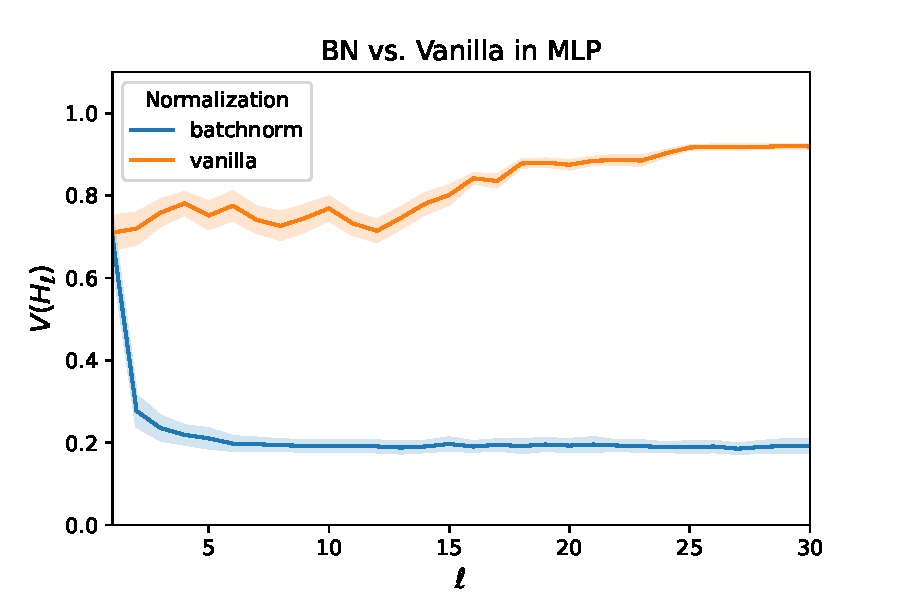
\includegraphics[width=\textwidth]{figures/Fig6A.pdf}
%           \caption{MLP}
%           \label{ortho:fig:relu_mlp}
%       \end{subfigure}
%       \begin{subfigure}[b]{0.4\textwidth}
%           \centering         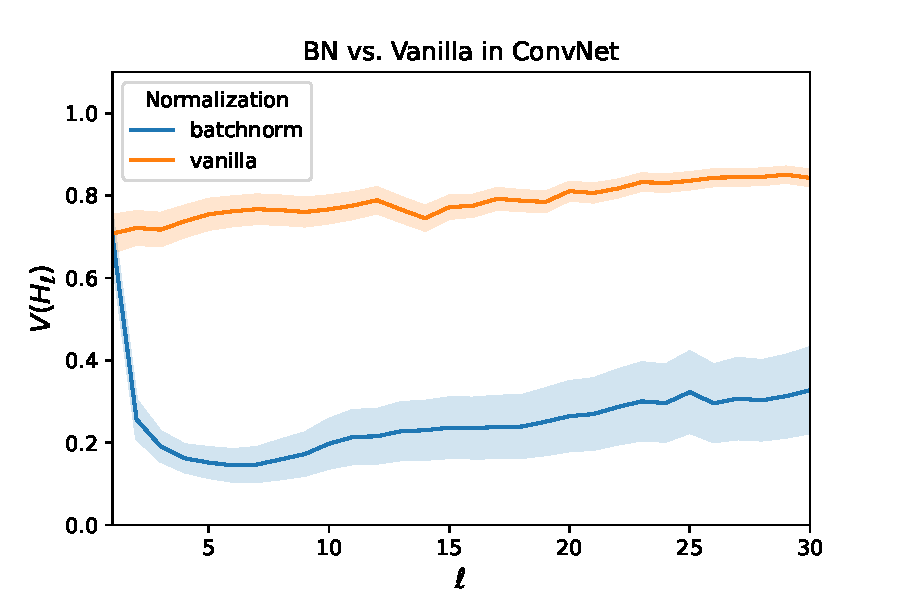
\includegraphics[width=\textwidth]{figures/Fig6B.pdf}
%           \caption{ConvNet}
%           \label{ortho:fig:convnet}
%       \end{subfigure}
%          \caption{Orthogonality gap of layers for BatchNorm vs vanilla network with ReLU, for MLP and a basic convolutional network on CIFAR10. Batch size was set to $8$, the number of hidden layers for both networks was set to $30$, with $100$ width for MLP and $100$ channels for ConvNet in all hidden layers. For the ConvNet, the kernel size was set to $3$, across all hidden layers, with zero-padding to make convolutional feature maps equal sized. The standard deviations were computed for $50$ different randomly sampled batches.}
%          \label{ortho:fig:relu_convnet}
%  \end{figure}
%  For an arbitrary activation function $F$, the hidden representations make the following Markov chain: 
%  \begin{align*}
%      Q_{\ell+1} = BN'(W_\ell F(Q_\ell)).
%  \end{align*}
%  where we assume that $BN'$ makes rows of its input matrix zero-mean and unit variance (the mean correction is included).
%  \subsubsection*{Conjecture}
%  Suppose that $\{ Q_\ell \}$ is \textit{ergodict} \citep{eberle2009markov}, and admits a unique invariant distribution denoted by $\nu$. We define function $L:\R^{d\times n}\to \R_+$ as
%  \begin{align}
%       L(Q_\ell)  = \left\| Q_\ell^\top Q_\ell - \E_{Q\sim \nu} \left[  Q^\top Q \right] \right\|_F .
%  \end{align}
%  We conjecture that there exists an integer $k$ such that for $\ell>k$ the following holds: 
%  \begin{align}
%      \E \left[ L(Q_\ell) \right] =\bigo\left( \frac{1}{ \sqrt{d}} \right).
%  \end{align}
%  Figure~\ref{ortho:fig:activations} experimentally validates that the above result holds for standard activations such as ReLU, sigmoid, and tanh. 
 
%  \begin{figure}[!ht]
%      \centering
%      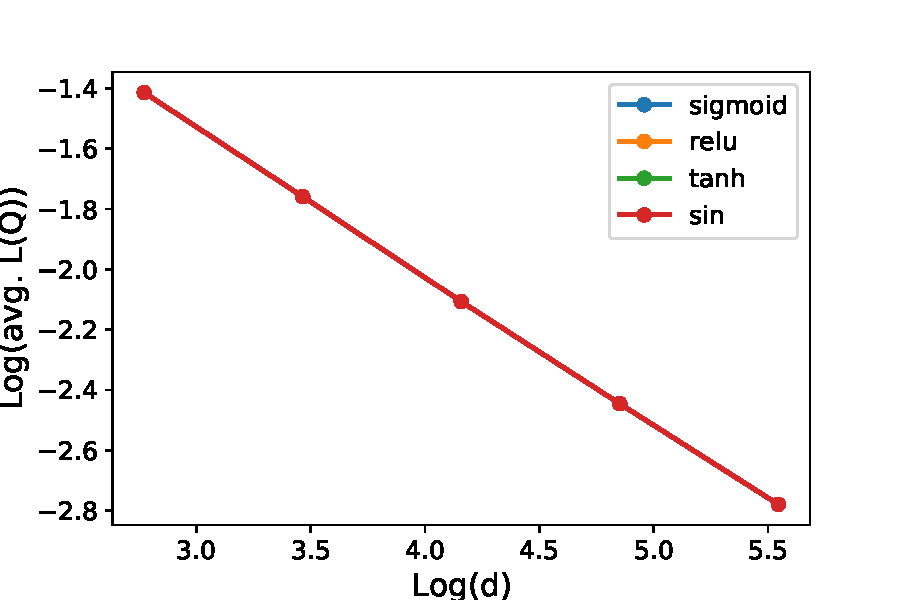
\includegraphics[width=0.45\textwidth]{figures/activations.pdf}
%      \caption{\footnotesize{\textbf{Validating the conjecture.} Horizontal axis: $\log(d)$; vertical axis: $\log(\frac{1}{1000}\sum_{k=1}^{1000} L(Q_k))$. The difference between the plots is negligible, hence not visible. }}
%      \label{ortho:fig:activations}
%  \end{figure}
 
 
 
  
 
%  \subsubsection*{Odd activations}
%  We observe that Theorem~\ref{ortho:thm:contraction} holds for odd activations such as $\sin$ and $\tanh$ with no need to the mean correction in BN. For these activation result of Theorem~\ref{ortho:thm:contraction}. 
%  \begin{align*}
%      \E \left[ V(H_{\ell+1}) \right]  = \bigo\left( (1-\alpha)^{\ell} + \frac{1}{\sqrt{d}}\right) 
%  \end{align*}
%  holds under \ref{ortho:assume:lineary_indepdence}$(\alpha,\ell)$. Remarkably, this is consistent with our conjecture with $ V = L$ for these activations.   



 \section{Comparisons with a BN-replacement}
 \label{ortho:sec:bnreplace}
 Here, we compare iterative orthogonalization with two baselines: (i) initialization with random orthogonal weights \citep{saxe2013exact}, and (ii) adaptive gradient clipping \citep{brock2021high}.
 \begin{itemize}
     \item[(i).] Orthogonal weights achieve orthogonal representations in deep \textit{linear} networks. Consider a MLP whose weight are initialized by Xavier's scheme. Let the weight matrix at layer $\ell$ admit the SVD decomposition $W_\ell = U_\ell \diag(\sigma_\ell) V_\ell$. Then, we replace the weight matrix by the orthogonal matrix $(\text{mean}(\sigma_\ell)) U_\ell V_\ell^\top $. Since ReLU networks with orthogonal weights are prone to the alignment of representations in deep layers, we observed that such an initialization does not help with the slow down of training with depth (see Fig.~\ref{ortho:fig:clipping1}).  
     \item[(ii).] Recently, \cite{brock2021high} propose an effective replacement for BN ---- based on gradient clipping. Let $G_\ell$ denotes the gradient of training loss with respect to $W_\ell$. Given a clipping parameter $\lambda$, adaptive gradient clipping adjusts the norm of $G_\ell$ as
     \begin{align}
         \widehat{G}_\ell = \begin{cases} 
         \left(\lambda \frac{\|W_\ell \|_F^*}{\| G_\ell \|_F}\right) G_\ell & \frac{\| G_\ell \|_F}{\| W_\ell \|_F^*} \geq \lambda \\ 
         G_\ell & \text{otherwise}
         \end{cases}
     \end{align}
     where $\| W_\ell \|_F^* = \max\{\| W_\ell \|_F, 10^{-2} \}$. 
 \end{itemize}
 Fig.~\ref{ortho:fig:clipping1}, and ~\ref{ortho:fig:clipping2} presents results for two different choice of clipping parameters $\lambda=0.1$ and $\lambda=1$, respectively. These plots demonstrate adaptive gradient clipping  effectively alleviates the training slow down with depth. Yet, we observe iterative orthogonalization achieves a better training loss after 30 epochs. 
 It is not known how the clipping enhance the training. While, iterative orthogonalization is inspired by orthogonalization of representations with BN layers, which is theoretically established in this chapter.
 \begin{figure}[!ht]
      \centering
      \begin{subfigure}[b]{0.3\textwidth}
          \centering        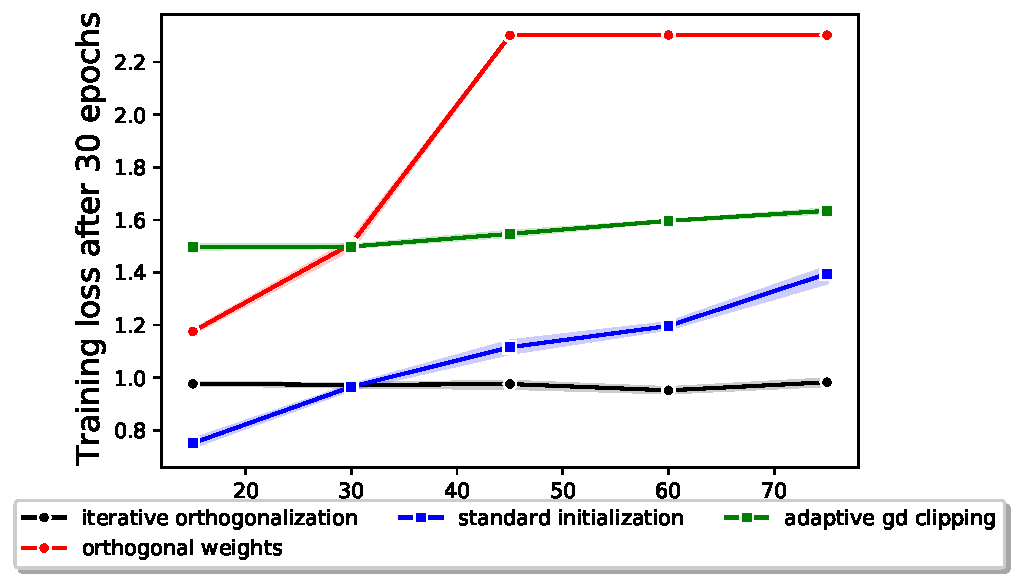
\includegraphics[width=\textwidth]{figures/baselines.pdf}
          \caption{$\lambda=0.1$}
          \label{ortho:fig:clipping1}
      \end{subfigure}
      \begin{subfigure}[b]{0.3\textwidth}
          \centering         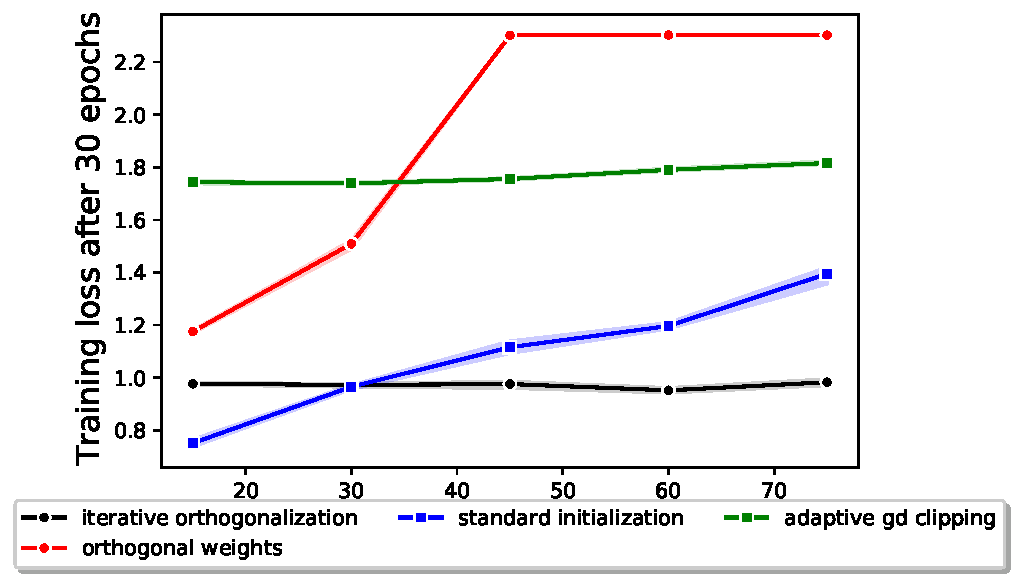
\includegraphics[width=\textwidth]{figures/baselines2.pdf}
      \caption{$\lambda=1$}
  \label{ortho:fig:clipping2}
      \end{subfigure}
         \caption{Iterative orthogonalization vs adaptive gradient clipping. Horizontal axis: the network depth. Vertical axis: training loss for each network after 30 SGD epochs. For more details, see Sec.~\ref{ortho:sec:optimization}.  Mean and 95\% confidence interval of 4 independent runs.}
 \end{figure}


%  \subsection*{Experiments for convolutional networks}
%  \label{ortho:sec:experiments}
%  The introduced initialization scheme in Section~\ref{ortho:sec:optimization} extends to convolutional networks.  In convolutional networks, hidden representation are in the tensor form $H_\ell \in \R^{d\times m \times m \times n}$ where $d$ is the number of filters and $k$ is the image dimensions. Let matrix $W_\ell^{d \times k^2}$ are weights of convolutions layer $\ell$ with kernel size $k$ and $d$ filters.  A 2D convolution is a matrix multiplication combined by a projection as:
%  \begin{align}
%      \text{conv2d}(W_\ell,H_\ell) = \text{fold}\left( W_{\ell} \underbrace{\text{unfold}(H_\ell)}_{H'_\ell}\right)
%  \end{align}
%  where the unfolding extract batches of $k\times k$ from images in tensor $H_\ell$, and folding operation combines the computed convolution for the extracted batches. 
%  We use the SVD decomposition $H'_\ell = U_\ell \Sigma_\ell V_\ell$ to initialize weights $W_\ell$, exactly the same as Eq.~\eqref{ortho:eq:init_w}: 
%  \begin{align*}
%      W_\ell = \frac{1}{\| \Sigma_\ell^{\sfrac{1}{2}}\|_F} V_\ell' \Sigma_\ell^{-\sfrac{1}{2}} U_\ell^\top,
%  \end{align*}
%  where $V_\ell'$ is a slice of $V_\ell$.
%   We experimentally validate the performance of this initialization for two convolution networks with ReLU activations consisting of 20 and 80 convolutions. Table~\ref{ortho:tab:convnet} outlines the details of these neural architectures. 
%  \begin{table}[!ht]
%      \centering
%      \begin{tabular}{|c|c|}
%      \hline
%         The network with 20 layers  &   The network with 80 layers \\
%         \hline
%         Conv2d(3, 64)+    MaxPool2d(2) + RELU 
%         & Conv2d(3, 64)+   MaxPool2d(2) + RELU  \\
%         Conv2d(64, 192) + MaxPool2d(2) + ReLU &  Conv2d(64, 192) + MaxPool2d(2) + ReLU \\
%         Conv2d(192, 256)
%         + Conv2d(256, 256) +ReLU & Conv2d(192, 256)
%          Conv2d(256, 256) + ReLU
%          \\ 
%          \hline 
%          $\{$Conv2d(256, 256)+ReLU$\} \times 16$ &  $\{$Conv2d(256, 256)+ReLU$\} \times 76$
%          \\ 
%          \hline
%          MaxPool2d(2) + ReLU & MaxPool2d(2) + ReLU \\ 
%          Dropout(0.5) + Linear(1024,4096) + ReLU & Dropout(0.5) + Linear(1024,4096) + ReLU \\ 
%          Dropout(0.5) + Linear(4096,4096) + ReLU & Dropout(0.5) + Linear(4096,4096) + ReLU \\ 
%          Linear(4096,10) & Linear(4096,10)
%          \\
%          \hline
%      \end{tabular}
%      \caption{\footnotesize{Convolutional networks used in the experiment.} These neural architectures are obtained by adding layers to AlexNet~\citep{srivastava2014dropout}. The kernel size is 3 for all the convolutional layers. }
%      \label{ortho:tab:convnet}
%  \end{table} 
 
%  \begin{figure}
%      \centering
%      \begin{tabular}{c c}
%          20 layers &  80 layers\\
%         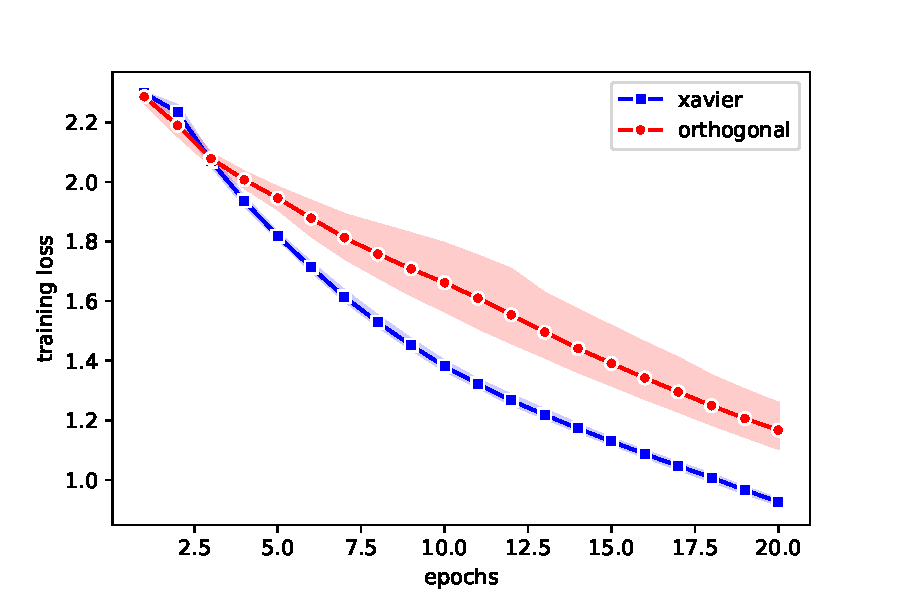
\includegraphics[width=0.4\textwidth]{figures/convolutional_15.pdf}  & 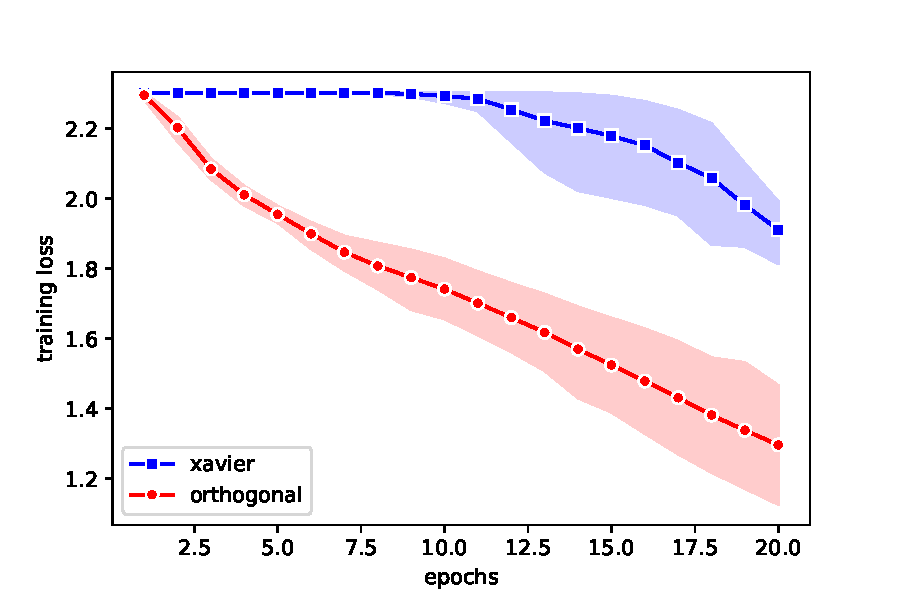
\includegraphics[width=0.4\textwidth]{figures/convolutional_75.pdf}
%      \end{tabular}
%      \caption{\footnotesize{\textbf{Training convolutional networks.} Convergence of SGD for Xavier's initialization \citep{glorot2010understanding} (in blue) and also the proposed initialization method that ensures the orthogonality of hidden representations (in red).  Mean and 95\% confidence interval of 4 independent runs.} }
%      \label{ortho:fig:convents}
%  \end{figure}
 
%  Figure~\ref{ortho:fig:convents} shows the performance of SGD (with stepsize $0.001$ and batchsize 30) for the proposed initialization. This initialization slows SGD for the shallow network with 20 layers compared to standard Xavier's initialization~\citep{glorot2010understanding}. However, it outperforms Xavier's initialization when the depth is significantly large. This result substantiates the role of orthogonality in training. We repeated this experimented for deeper networks and more epochs. Figure~\ref{ortho:fig:conv80} presents our results for a convolutional network with 90 layers and 80 epochs demonstrating orthogonal initialization boosts SGD performance even after many SGD epochs.  
 
 
 
 
%  Although the convolution network used in this experiment is not a conventional network, this experimental result motivates further investigations of the role of orthogonality in standard convolutional networks.
 
%  \begin{figure}
%      \centering
%      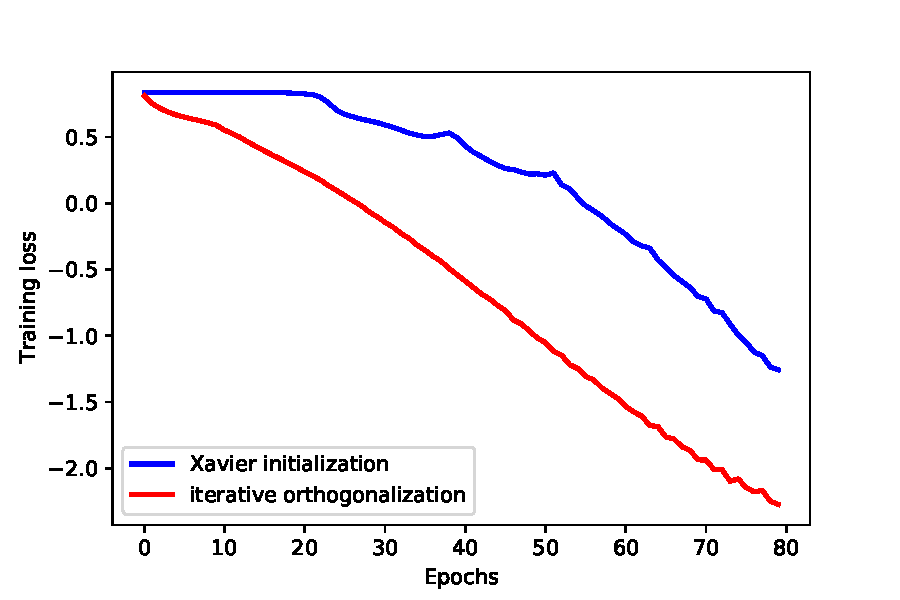
\includegraphics[width=0.5\textwidth]{figures/conv80.pdf}
%      \caption{\footnotesize{\textbf{Training convolutional networks.} Convergence of SGD for Xavier's initialization \citep{glorot2010understanding} (in blue) and also the proposed initialization method that ensures the orthogonality of hidden representations (in red).  Mean of 2 independent runs.} }
%      \label{ortho:fig:conv80}
%  \end{figure}
 
\chapter{Proof of Chapter~\ref{ch:bn_MF}}\label{ch:bn_MF:proofs}


\section{A concentration bound for the empirical covariance matrix}

The following analysis pertains to the deviation between the sample covariance matrix, normalized by the true covariance, and the identity matrix. For a collection of $d$ independent identically distributed \iid samples in $\R^d$, represented as $x_1, x_2, ..., x_d \in \R^n$, the sample covariance matrix $C_d$ is given by:

\begin{equation}
C_d = \frac{1}{d} \sum_{i=1}^{d} x_i x_i^T.
\end{equation}

The true covariance matrix $C$ is defined as the expected outer product of the samples, or:

\begin{align}
C = \mathbb{E}[x_i x_i^T].
\end{align}

We are interested in bounding the deviation of $ C_d$ from the covariance matrix $C$ in terms of their Frobenius norm (denoted as $\|.\|_{F}$), as outlined in the lemma below. Note that if activation $\act$ is uniformly bounded $\act(x)^2\le B x^2,$ and $\BN$ is the batch-norm operator, then ${\|\act(\BN(x))^2\|\le B \|\BN(x)\|^2 \le B n}.$ Thus, activations applied after normalization layers obey the condition of Lemma~\ref{MF:lem:sample_cov_deviation}. With this point in mind, we will prove the concentration result for vectors that are uniformly bounded by the same quantity.


\begin{lemma}\label{MF:lem:sample_cov_deviation}
Let $x_1,\dots,x_d\in \R^n$ be \iid random vectors with covariance $\E x_i x_i^\top = C$ and sample covariance $C_d:=\frac1d \sum_{i=1}^d x_i x_i^\top.$ If the vector norms are universally bounded such that $\norm{x_i}^2\le n \distort  $ holds almost surely, then for $t \lesssim \sqrt{d}$, the following is true:
\begin{align}
P\left(\|C_d - C\|_F \gtrsim t \eps \right) \leq \exp(-t^2), && \eps:=\frac{B n}{\sqrt{d}}.
\end{align}
Here, the probability is taken over the random vectors $x_1,\dots,x_d.$
\end{lemma}

We will use the last lemma to prove Theorem~\ref{MF:thm:concentration}.

\begin{lemma}\label{MF:lem:sample_cov_inv_deviation}
Under the same conditions as Lemma~\ref{MF:lem:sample_cov_deviation}, if the covariance matrix $C$ is not degenerate, i.e., it does not possess zero eigenvalues, for $t \lesssim \sqrt{d}$ it holds
\begin{align}
P\left(\|C^{-1} C_d - I_n\|_F \gtrsim t \eps \right) \leq \exp(-t^2), && \eps:=\frac{B\norm{C^{-1}} n}{\sqrt{d}}.
\end{align}
\end{lemma}

\begin{proof}[Proof of Lemma~\ref{MF:lem:sample_cov_deviation}]
Recall that Bernstein's inequality provides an upper bound on the probability that the sum exceeds a certain threshold $t$. Given \iid variables $X_1,\dots,X_d,$ it states that are uniformly bounded $|X_i|\le B$ for all $i$, we have
\begin{align}
\P\left(\frac{1}{d} \sum_{i=1}^{d} X_i\geq t\right) \leq 2 \exp\left(-\frac{dt^2/2}{K^2 + Kt/3}\right),
\end{align}
where $t > 0$ and $\sigma^2$ is the variance of $\sum_{i=1}^{d} E[ X_i^2] \le d B^2 $. 
Define $X_i:=\|x_i x_i^\top - C\|_F^2.$ We have
\begin{align}
    \|x_i x_i^\top - C\|_F^2 &\le \|x_i x_i\|_F + \|C\|_F\\
    &\le B n + \|E x_i x_i^\top \|_F\\
    &\le B n + E \|x_ix_i\|_F\\
    &\le 2 B n.
\end{align}
% \end{align}
Thus, we can plug $K:= 2 B n $ into the Bernstein's inequality to get 
\begin{align}
&\P\left(\frac1d\sum_{i=1}^{d} \|x_i x_i^\top - C\|_F \geq t\right) \leq\\
&\qquad \exp\left(-\frac{dt^2/2}{ 4 n^2\distort^2 + 2\distort n t/3}\right).
\end{align}
Since $\|\cdot\|_F $ is convex, Jensen's inequality which implies that moving the averaging inside can only decrease its value, which in turn implies 
\begin{align}
&\P\left(\|\frac1d\sum_{i=1}^{d}  x_i x_i^\top - C\|_F \geq t\right)\\
&\qquad \leq \exp\left(-\frac{d t^2}{ 8 n^2\distort^2 (1 + \frac{t}{6n\distort})}\right).
\end{align}
We can now rename $t \sqrt{d}/(\sqrt{8} B n)$ as $t$ and use definition of sample covariance to conclude 
\begin{align}
    \P\left(\|C_d - C\|_F \ge t \frac{\sqrt{8} B n}{\sqrt{d}}\right)\le \exp\left(- \frac{t^2}{(1+\frac{t}{3\sqrt{2 d}})}\right),
\end{align}
which can be restated as
\begin{align}
 \P\left(\|C_d - C\|_F \gtrsim t \eps\right)\le \exp(- t^2), &&  \eps:=\frac{ B n}{\sqrt{d}},
\end{align}
which holds if $t \lesssim \sqrt{d}.$
\end{proof}


\begin{proof}[Proof of Lemma~\ref{MF:lem:sample_cov_inv_deviation}]
Consider transformed vectors $z_i:=C^{-1/2} x_i.$ Note that we have $\E z_i z_i^\top = C^{-1} C = I_n.$ Thus, we can apply Lemma~\ref{MF:lem:sample_cov_deviation} on deviations of sample covariance of $z_i$'s from $I_n.$ Furthermore, we have $\norm{z_i}^2 \le \norm{C^{-1}} \norm{x_i}^2 \le \norm{C^{-1}} B n.$ So we can invoke Lemma~\ref{MF:lem:sample_cov_deviation} by setting $B$ to $\norm{C^{-1}}B .$
\end{proof}

\section{Analyzing Gram Dynamics Around Fixed Points}

Equipped  with the results established so far, we now turn our attention to the dynamics of Gram matrices in relation to the total variation of the Multi-Layer Perceptron (MLP) Markov chain. In particular, we demonstrate a specific construction based on fixed-point $G_*,$ and show that after one layer update the total variation distance is bounded.

% Recall the fixed point $\C$, $T$ in Equation \eqref{MF:eq:dist_recurrence}. Given a random representation $ h\in\R^{d\times n}$ drawn from $h\sim \mu$ \textcolor{blue}{what is $\mu$? shouldn't be $\mu_*$} and Gaussian weights $W\in\R^{d\times d}$ drawn \iid from $\Normal(0,1/d)$, the distribution of $h':=W \act(\BN(h))$ can be obtained by applying the Markov transition to $\mu_{h'}=T(\mu)$. The following Lemma bounds the $tv(h,h')$, thereby proving that the distribution $h$ is almost an invariant distribution for wide neural networks. 

\begin{lemma}[Restated Lemma~\ref{MF:lem:tv_one_step}]\label{MF:lem:one_step_restated}
    Let $\hat h\in\R^{d\times n}$ be constructed by drawing its rows \iid from $\Normal(0,G_*)$. Let $\hat\mu$ denote the distribution of $\hat h$. Given that fixed-point Gram matrix $G_*$ is non-degenerate and the activation is uniformly bounded $\act(x)^2 \le B x^2$, then
    \begin{align}
        \norm{\hat\mu - T(\hat \mu)}_{tv} \lesssim \eps^2 \LN(1/\eps), && \eps:=\frac{n\norm{G_*^{-1}}\distort }{\sqrt{d}},
    \end{align}
    holds if $B$ and $\norm{G_*^{-1}}$ are non-zero. 
\end{lemma}


Under the assumption of geometric contraction, irrespective of the initial distribution, the total variation distance to the stationary distribution contracts by $1-\alpha$, for some $\alpha>0$, after one transition $T$. This result, together with Lemma~\ref{MF:lem:tv_one_step}, provides a tool to approximate the stationary distribution by a matrix constructed from the fixed-point Gram matrix $G_*$.

\begin{lemma}\label{MF:lem:stationary_dist_approximation}
    Let $\hat\mu$ denote the distribution of a random matrix in $\R^{d\times n}$, whose rows are drawn \iid from $\Normal(0,G_*)$. Assuming the rapid mixing condition~\ref{MF:ass:rapid_mixing} holds with constant $\alpha> 0$, then
    \begin{align}
        \norm{\hat\mu-\mu_*}_{tv}\lesssim \alpha^{-1}\eps^2\LN(1/\eps), && \eps:=\frac{n\distort \norm{G^{-1}_*}}{\sqrt{d}}.
    \end{align}
\end{lemma}

We can finally the results about total variation into the context of Gram matrix dynamics through depth.
\begin{lemma}\label{MF:lem:multiple_steps_total_variation}
    Let $\mu_\ell$ denote the hidden representation of a BN-MLP, and $\hat\mu$ denote the distribution of a matrix whose rows are drawn from $\Normal(0,G_*)$. If hidden representations obey the rapidly mixing assumption with rate $1-\alpha,$ for $\alpha>0,$ then 
    \begin{align}
        \norm{\mu_\ell-\hat\mu}_{tv}\lesssim (1-\alpha)^\ell + \alpha^{-1}\eps^2\LN(1/\eps), && \eps:=\frac{n\distort\norm{G_*^{-1}}}{\sqrt{d}}.
    \end{align}
\end{lemma}





With the necessary lemmas in place, we are now ready to present our main theorem.

\begin{theorem}[Restated Theorem~\ref{MF:thm:concentration}]\label{MF:thm:concentration_restated}
For an MLP chain $G_\ell$ that originates from a non-degenerate input $G_0,$ and that has a non-degenerate fixed point $G_,$ and that obeys the rapidly mixing assumption with $\alpha>0,$ we have the following:
\begin{align}
    &\P(\|G_* - G \|_F \ge t)\lesssim \nonumber\\
    &\qquad t^{-2}(\|G_*\|^2 (1-\alpha)^\ell + \alpha^{-1} \eps^2 \LN(1/\eps)),
\end{align}
with $\eps:= n B \kappa(G_*)/\sqrt{d}.$ 
\end{theorem}

The proof of the theorem relies on the following lemma bounds Gram matrix deviations by total variation.

\begin{lemma}\label{MF:lem:total_variation_lower_bound}
Conditioned on Gram matrices $G_*,G\in\R^{n\times n},$ construct $h, \hat h\in\R^{d\times n}$ by drawing their rows \iid from $\Normal(0,G)$ and $\Normal(0,G_*).$ If $G_*$ is non-degenerate, the following hols for total variation between $h$ and $\hat h$:
\begin{align}
    \TV(h,\hat h)\ge \frac{t}{100}\P(\|G_*^{-1} G - I_n\|_F^2 \ge t),
\end{align}
where the probability is defined over $G.$
\end{lemma}

The proof of this theorem follows directly from the lemmas we have established. 

\begin{proof}[Proof of Theorem~\ref{MF:thm:concentration_restated}]
We apply the total variation bound established in Lemma~\ref{MF:lem:multiple_steps_total_variation} and combine this with the lower bound stated in Lemma~\ref{MF:lem:total_variation_lower_bound} 
\begin{align}
    &\frac{t}{100}\P(\|G_*^{-1} G - I_n\|_F^2 \ge t)\\
    &\qquad \le \TV(h_\ell,\hat h)\lesssim (1-\alpha)^\ell + \alpha^{-1} \eps^2 \LN(1/\eps) .\label{MF:eq:main_inequality}
\end{align}
Omitting constants we have
\begin{align}
    &\P(\|G_*^{-1} G - I_n\|_F \ge \sqrt{t})\\
    &\quad \qquad \lesssim t^{-1}((1-\alpha)^\ell + \alpha^{-1} \eps^2 \LN(1/\eps)).
\end{align}
By a change of variables we get
\begin{align}
    &\P\left(\|G_*^{-1} G - I_n\|_F \ge t\right)\\
    &\qquad \lesssim t^{-2}((1-\alpha)^\ell + \alpha^{-1} \eps^2 \LN(1/\eps)).
\end{align}
Note that $\|G^* - G \|_F = \|G^*(G^{-1}_* G - I_n)\|_F,$ which is bounded by $\|G_*\|\|G^{-1}_* G- I_n\|_F.$ Thus
\begin{align}
    &\P\left(\|G_* - G \|_F \ge t\right) \\
    &\quad \le \P\left(\|G_*^{-1} G - I_n\|_F \ge t/\|G_*\|\right) \\
    &\quad \le t^{-2} \|G_*\|^2 ((1-\alpha)^\ell+ \alpha^{-1}\eps^2\LN(1/\eps)),
\end{align}
where the last equation is due to \eqref{MF:eq:main_inequality}. The above inequality obtains
\begin{align}
& \eps:=\frac{ B n }{\sqrt{d}}\|G_*\|\|G_*^{-1}\|\\
  &  \P(\|G_* - G\|_F \ge t)\lesssim \\
  &\qquad \qquad t^{-2}\left( \|G_*\|^2 (1-\alpha)^\ell + \alpha^{-1}\eps^2\LN(1/\eps))\right).
\end{align}
Recall that $\|G_*\|\|G_*^{-1}\|$ encodes the ratio of largest to smallest eigenvalue of $G_*,$ which is its condition number $\kappa(G_*).$ This finalizes the proof. 
\end{proof}


% \begin{proof}
%     We can invoke the total variation bound of Lemma~\ref{MF:lem:multiple_steps_total_variation} and leverage the lower bound of total variation by deviation from identity in Lemma~\ref{MF:lem:total_variation_lower_bound} to conclude the proof. 
% \end{proof}



\begin{proof}[Proof of Lemma~\ref{MF:lem:multiple_steps_total_variation}]
First, note that geometric contraction assumption implies
\begin{equation}
    \tv{\ell}{*}\le (1-\alpha)\tv{\ell-1}{*} \le (1-\alpha)^\ell,
\end{equation}
which by numerical inequality $1-x\le \exp(-x)$ can be bounded by $\exp(-\alpha \ell).$ We can invoke Lemma~\ref{MF:lem:stationary_dist_approximation} and triangle inequality for total variation to conclude the proof.
\end{proof}

\begin{proof}[Proof of Lemma~\ref{MF:lem:stationary_dist_approximation}] 
Recall that the rapidly mixing assumption implies that $\norm{T(\hat\mu)-\mu_*}_{tv}\le (1-\alpha) \norm{\hat\mu-\mu_*}_{tv}.$ Furthermore, invoking Lemma~\ref{MF:lem:one_step_restated}, we have 
\begin{align}
    \norm{T(\hat\mu)-\hat\mu}_{tv}\lesssim \eps^2\LN(1/\eps),\\
  \implies  \norm{\hat\mu-\mu_*}_{tv}\lesssim \alpha^{-1} \eps^2\LN(1/\eps),
\end{align}
where the last line is implied by the triangle inequality for total variation.
\end{proof}


\begin{proof}[Proof of Lemma~\ref{MF:lem:one_step_restated}]
Let us explicitly construct $T(\hat \mu).$ Recall that $\hat\mu$ describes distribution of $\hat h$ whose rows are drawn \iid from $\Normal(0,G_*).$ Define $h:=W \act(\BN(\hat h)),$ where $W$ is a Gaussian with \iid elements $\Normal(0,1/d).$ Thus, by construction, distribution of $h$ follows $T(\hat \mu).$ Our main proof strategy of upper bounding total variation between $\hat h$ and $h$ is to bound it conditioned on the proximity of $G$ to $G_*.$ 

\textbf{Bounding deviations $\|G_*^{-1} G - I\|_F$.}
Recall that based on the fixed-point property of $G_*$ we have 
\begin{align}
    \E_{w\sim N(0,G_*)} \act(\BN(w))^{\otimes 2} = G_*.
\end{align}
Define sampled Gram of activations $G:= \frac1d \act(\BN(\hat h))^\top \act(\BN(\hat h)),$ which is equal in expectation to $\E G = G_*.$ By construction of batch norm operator which maps every row to $\sqrt{n}$-sphere, and the uniform bound $\act(x) ^ 2 \le B x^2, $ we can conclude that rows of $\act(\BN(\hat h))$ are always bounded by 
\begin{align}
    &\|\BN(x)\| \le \sqrt{n} && \forall x\in\R^n\\
  \implies  &\|\act(\BN(x))\| \le \sqrt{B n }, && \forall x\in\R^n\\
  \implies  &\|\row_k(\act(\BN(\hat h)))\|^2 \le B n, && \forall k.
\end{align}
This allows us to invoke Lemma~\ref{MF:lem:sample_cov_inv_deviation} to conclude:
\begin{align}
    \P(\|G_*^{-1} G - I_n\|_F \ge t\eps ) \le \exp(-t^2),
\end{align}
where $\eps = B \|G_*^{-1}\| n/\sqrt{d}.$ 


\textbf{Bounding total variation $\TV(h,\hat h).$} Define set of matrices $N_t:=\{M\in\R^{n\times n}: \norm{\C^{-1}M- I_n}_F^2\le \eps^2 t^2 \}.$ 
% Define Gram matrix $G :=\frac1d \act(\BN(h))\act(\BN(h))^\top$. 
Observe that conditioned on $G$, $h$ is equal in distribution to a matrix rows are drawn \iid from $\Normal(0,G)$. Thus, we can decompose the total variation based on depending on $G$ belonging to neighborhood of $G_*$ or not 
\begin{align}
    \TV(h, \hat h)
    &\le \Prob{\norm{\C^{-1}\Csa-I_n}_F^2 \ge t^2\eps^2 } \\
    & \qquad +  \sup_{G\in N_t}\TV(\Normal(0,G),\Normal(0,G_*))\\
    & \lesssim \Prob{\norm{\C^{-1}\Csa-I_n}_F \ge t\eps} + \frac{3}{2}t^2 \eps^2 ,
\end{align}
where in the last line we use the upper bound on total variation between two Gaussian matrices from~\cite{devroye2018total}. Plugging our result for deviation of $G$ and $G_*$ we have
\begin{align}
    \TV(h, \hat h)\le \frac{3}{2}t^2 \eps^2 + \exp(-t^2),
\end{align}
which holds for all $t \lesssim \sqrt{d}.$ In particular, we can set $t^2:=\LN(2/3\eps^2)$ which implies
\begin{align}
    \TV(h, \hat h) \lesssim \frac{3\eps^2}{2}(1+\LN(2/2\eps^2)),
\end{align}
which omitting constants can be restated as 
\begin{align}
    \TV(h, \hat h) \lesssim \eps^2\LN(1/\eps^2).
\end{align}
To finish the proof, observe that condition $t\lesssim \sqrt{d}$ translates to $\LN(1/\eps^2)=O(d)$ which in turn requires $\eps \gtrsim \exp(-d/2).$ Plugging the definition of $\eps$ we have $n B \|G_*^{-1}\|\gtrsim \sqrt{d} \exp(-d/2).$ Since the right-hand side is $o(1),$ and $n\ge 1,$ this condition will always hold if the boundedness and conditioning are non-zero $B,\| G_*^{-1}\| > 0.$
% By a change of variable and omitting the absolute constants, we have
% \begin{align}
%     \norm{\hat\mu - T(\hat\mu)}_{tv} &\lesssim \eps\LN(1/\eps), && \eps:=\frac{n\distort\norm{G_*^{-1}}}{\sqrt{d}}.
% \end{align}
% Finally, recall the condition for $t/n\distort\le 3/4$, which is equivalent to $\eps \lesssim n\distort ,$ which holds for $\epsilon \lesssim 1.$ For $\eps > 1,$ since the total variation distance is always bounded by $1,$ the inequality becomes vacuous and always true. Thus, the inequality holds for arbitrary $\eps>0.$
\end{proof}


\begin{proof}[Proof of Lemma~\ref{MF:lem:total_variation_lower_bound}]
Define set of matrices $N_t:=\{M\in\R^{n\times n}: \norm{\C^{-1}M- I_n}_F^2\le t \}$. We have
\begin{align}
    \TV(h,\hat h) &= \int_G \P(G)\TV(\Normal(0,G),\Normal(0,G_*)) \\
    & = \int_{G\in N_t} \P(G)\TV(\Normal(0,G),\Normal(0,G_*)) \\
    &\qquad + \int_{G\notin N_t} \P(G)\TV(\Normal(0,G),\Normal(0,G_*)) \\
    &\ge \int_{G\notin N_t} \P(G)\TV(\Normal(0,G),\Normal(0,G_*)) \\
    &\ge \P(G \notin N_t) \inf_{G\notin N_t}\TV(\Normal(0,G),\Normal(0,G_*))\\
    &\ge \frac{t}{100} \P\left(\norm{G_*^{-1}G-I_n}_F^2\ge t\right),
\end{align}
where in the last line we have used the lower bound for total variation of multivariate Gaussians from~\cite{devroye2018total}.
\end{proof}

\chapter{Supplemental proofs and experiments for Chapter~\ref{ch:bn_grad}}




\section{Conditional orthogonalization}
% \input{sections/appendices/conditional_orthogonalization}
\paragraph{Isometry after rotation.}
Our analysis is based on ~\citep[Corollary 3]{joudaki2023impact}, which we restate in the following Lemma:
\begin{lemma}
    \label{grad:lem:isobn}
    For all non-degenerate matrices $X \in \R^{d \times d}$, we have:
    \begin{align}
        \I(\BN(X))\geq \left(1+ \frac{\text{variance}\{\|X_{j\cdot}\|\}_{j=1}^d}{(\text{mean} \{\|X_{j\cdot}\|\}_{j=1}^d)^2}\right) \I(X)~.
    \end{align}
\end{lemma}

Lemma~\ref{grad:lem:isobn} proves isometry bias of $\BN$. The next lemma proves that isometry does not change under rotation  

\begin{lemma}[Isometry after rotation]
% \label{grad:lem:iso_rotation}
Let $X \in \R^{d\times d}$ and $W \sim \mathbb{O}_d$ be a random orthogonal matrix and $X'= W X$. Then,  
\begin{align}
   \I(\BN(X'))\geq \left(1+ \frac{\text{variance}\{\|X'_{j\cdot}\|\}_{j=1}^d}{(\text{mean} \{\|X'_{j\cdot}\|\}_{j=1}^d)^2}\right) \I(X)~.
\end{align}
\end{lemma}
%
\begin{proof}
   Using properties of the determinant, we have 
   \begin{align}
       \det(X' X'^\top ) = \det(W)^2 \det(XX^\top) =  \det(XX^\top),
   \end{align}
   where the last equation holds since $W$ is an orthogonal matrix. Furthermore, 
   \begin{align}
    \tr(X' X'^\top) & = \tr(W X X^\top W^\top ) \\
    & = \tr(XX^\top \underbrace{W^\top W}_{=I}) \\
    & = \tr(XX^\top)~.
   \end{align}
Combining the last two equations with Lemma~\ref{grad:lem:isobn} concludes the proof.
\end{proof}

\paragraph{Increasing isometry with rotations and $\BN$.}
The last lemma proves the isometry bias does not decrease with rotation and $\BN$. However, this does not prove a strict decrease in isometry with $\BN$ and rotation. The next lemma proves there exists an orthogonal matrix for which the isometry is strictly increasing. 
\begin{corollary}[Increasing isometry]
\label{grad:cor:isometry_increase}
Let $X \in \R^{d\times d}$ and denote its singular value decomposition $X = U \diag\left(\{\sigma_i\}_{i=1}^d\right) V^\top$, where $U$ and $V$ are orthogonal matrices. Then, we have:
\begin{align}
    \I (\BN(U^\top H)) = 1~.
\end{align}
\end{corollary}
%
\begin{proof} 
Let $S = \diag \left(\{\sigma_i\}_{i=1}^d \right)$ be the diagonal matrix containing the singular values of $X$. Then, we have:
\begin{align}
    \BN(U^\top X) &= \BN(U^\top U S V^\top) \\
    &= \BN(S V^\top) \\
    &= \diag(SV^\top V S)^{-\frac{1}{2}} SV^\top \\
    &= S^{-1} S V^\top \\
    &= V^\top,
\end{align}
which has maximum isometry 1 since it's an orthonormal matrix.
\end{proof}

Thus, there exists a rotation that increases isometry with $\BN$ for each non-orthogonal matrix.
 The proof of the last corollary is based on a straightforward application of Lemma~\ref{grad:lem:iso_rotation}.



\paragraph{Orthogonalization with randomness.}
The isometric is non-decreasing in Lemma~\ref{grad:lem:iso_rotation} and provably increases for a certain rotation matrix (as stated in the last corollary). Hence, it is possible to increase isometry with random orthogonal matrices. 

\begin{theorem}
    % \label{grad:thm:iso_bound}
    Suppose $W \sim \mathbb{O}_d$ is a matrix drawn from $\mathbb{O}_d$ such that $W\stackrel{d}{=} WU$ for all orthogonal matrices $U$. Let $\{\lambda_i\}_{i=1}^d$ be the eigenvalues of $XX^\top$. Then,
    \begin{align}
        \E_W \left[\I(\BN(WX))\right | X] \geq \left( \frac{1}{ 1 - \frac{\sum_{k=1}^d (\lambda_k - 1)^2}{2d^2(d+2)} } \right) \I(X)   
    \end{align}
    holds for all $X = \BN(\cdot)$, with equality for orthogonal matrices.
\end{theorem}
\begin{remark}
    Note that the assumption on $X=\BN(\cdot),$ can be viewed as an induction hypothesis, in that we can recursively apply this theorem to arrive at a quantitative rate at depth. 
\end{remark}
Notably, $\sum_{i=1}^d \lambda_i = d$ if $X = \BN(\cdot)$. Hence, one can expect that $\sum_{i=1}^d \lambda_i^2 < d^2$ for all full random matrices $X$ in form of $X = \BN(\cdot)$. 

\begin{proof}
We need to compute the variance/mean ratio in Lemma~\ref{grad:lem:iso_rotation}.
Let $X \in \R^{d \times d}$ have SVD decomposition $X = U \diag\{\sigma_i\}_{i=1}^d V^\top$ where $U$ and $V$ are orthogonal matrix and $\sigma_i^2 = \lambda_i$. Since the distribution of $W$ is invariant to transformations with orthogonal matrices, the distribution of $W$ equates those of $X' = W \diag\{\sigma_i\} V^\top$. It easy to check that 
\begin{align}
    \| X_{j\cdot}' \| = \sqrt{\sum_{i=1}^d \sigma_i^2 W_{ji}^2 } = \sqrt{\sum_{i=1}^d \lambda_i W_{ji}^2 }~.
\end{align}
Thus, 
\begin{align}
    \sum_{j=1}^d \| X_{j\cdot}' \|^2 = \sum_{i=1}^d \lambda_i = d, 
\end{align}
where the last equality holds due to the batch normalization.
Thus, we have
\begin{equation}
   \label{grad:eq:proof_iso_bound_eq1}
   \E \left[ \frac{d\sum_{j=1}^d \|X'_{j \cdot} \|^2}{(\sum_{j=1}^d \| X'_{j \cdot} \|)^2} \right] 
   = \E \left[\frac{d^2}{(\sum_j \| X'_{j \cdot} \|)^2} \right] 
   \geq \frac{d^2}{\E \left[ \left(\sum_{j=1}^d \| X'_{j \cdot} \|\right)^2 \right]}~.
\end{equation}
We need to estimate 
\begin{align}
    \E \left[ \| X_i'\| \| X_j'\| \right] = \E \left[ \left(\sum_{k=1}^d \lambda_k W_{ik}^2\right)^{\frac{1}{2}} \left(\sum_{k=1}^d \lambda_k W_{jk}^2\right)^{\frac{1}{2}}\right]~. 
\end{align}
Since square root function is concave, we have $\sqrt{x} \leq 1 + \frac{1}{2} (x-1)$.
Thus 
\begin{align}
    \E \left[\| X'_i \| \| X'_j\| \right]
& \leq \E \left[\left(1 + 0.5 \sum_{k=1}^d (\lambda_k-1) W_{ik}^2 \right) \left(1 + 0.5 \sum_{k=1}^d (\lambda_k-1) W_{jk}^2\right)\right] \\ 
& = 1 + \frac{1}{4} \sum_{k, q} (\lambda_k-1)(\lambda_q -1) \E \left[W_{ik}^2 W_{jq}^2 \right] \\
&= 1 + \frac{1}{4}\left[ \sum_{k \neq q} (\lambda_k-1)(\lambda_q -1)\underbrace{\E \left[ W_{ik}^2 W_{jq}^2 \right]}_{E_1} + \sum_{k=q} (\lambda_k-1)(\lambda_k -1)\underbrace{\E \left[ W_{ik}^2 W_{jk}^2 \right]}_{E_2} \right],
\end{align}
where in the first equality we have used the fact that the cross terms reduce, where the expectations are applications of Weingarten calculus:
\begin{align}
    \E \left[ 0.5 \sum_{k=1}^d(\lambda_k - 1)W_{ik}^2 + 0.5 \sum_{k=1}^d(\lambda_k - 1)W_{jk}^2 \right]
    &= \E \left[ 0.5 \sum_{k=1}^d \lambda_k W_{ik}^2  + 0.5 \sum_{k=1}^d \lambda_k W_{jk}^2 - 1 \right] \\
    &= 0.5 \sum_{k=1}^d \lambda_k \E \left[W_{ik}^2 \right] + 0.5 \sum_{k=1}^d \lambda_k \E \left[W_{jk}^2 \right] - 1 \\
    &= \frac{0.5}{d} \sum_{k=1}^d \lambda_k  + \frac{0.5}{d} \sum_{k=1}^d \lambda_k - 1 \\
    &= 0~.
\end{align}

The main quantity we must compute is an expectation of polynomials taken over the Haar measure of the Orthogonal group $O(n)$. To carry out the computation, we make use of Weingarten calculus~\citep{banica2011polynomial, collins2006integration, weingarten1978asymptotic}. More specifically, we make use of the of the Weingarten formula, studied by~\cite{collins2006integration, collins2022weingarten}:
\begin{align}
    \int_{O(n)} r_{i_1 j_1} r_{i_2 j_2} \dots r_{i_{2d} j_{2d}} d\mu(O(n)) = \sum_{\sigma \in \mathcal{M}_{2d}} \sum_{\sigma \in \mathcal{M}_{2n}} \Delta_\sigma(\boldsymbol{i}) \Delta_\sigma(\boldsymbol{j}) \wg^O(\sigma^{-1}\tau),
\end{align}
where $\mu(O(n))$ is the Haar measure of Orthogonal group. For an in depth explanation of each quantity in the Weingarten formula, we refer the reader to  \citet[Section 5.2]{collins2022weingarten}.

The quantity we focus on is $\E_W \left[W_{ik} W_{ik} W_{jq} W_{jq}\right]$. We will do the computation on multiple cases, based on the equalities of $k, q$. Notice that $i \neq j$ in all cases. It suffices if we focus on the two distinct cases: $E_1 = \E_W \left[W_{ik}^2  W_{jq}^2\right]$ $(k \neq q)$ and $E_2 = \E_W \left[W_{ik}^2  W_{jk}^2\right]$ $(k = q)$.

% We rewrite the expression as $\E_W \left[W_{i \alpha}^2 W_{j \beta}^2 \right] = \E_W \left[W_{i \alpha} W_{i \alpha} W_{j \beta} W_{j \beta} \right]$, where $\alpha, \beta$ will be replaced by all combinations of the indices.

We first compute $E_1$.

Following the procedure from \citet[Section 5.2]{collins2022weingarten}, we take the index sequences to be $\boldsymbol{i} = (i, i, j, j)$ and $\boldsymbol{j} = (k, k, q, q)$. Similarly, we get $\Delta_\sigma(\boldsymbol{i}) = \Delta_{\tau}(\boldsymbol{j}) = 1$ only if $\sigma = \{ \{1, 2\}, \{3, 4\} \}$ and $\tau = \{ \{1, 2\}, \{3, 4\} \}$. 

Consdering $\sigma, \tau$ as permutations, we get:
\begin{align}
    \sigma &= \begin{pmatrix}
                1 & 2 & 3 & 4\\
                1 & 2 & 3 & 4
                \end{pmatrix},  \\
    \tau &= \begin{pmatrix}
                1 & 2 & 3 & 4\\
                1 & 2 & 3 & 4
                \end{pmatrix}, \\
    \sigma^{-1} \tau &= \begin{pmatrix}
                1 & 2 & 3 & 4\\
                1 & 2 & 3 & 4
                \end{pmatrix},
\end{align}
where $\sigma^{-1} \tau$ has coset-type $[1, 1]$. Finally, we plug the results back into the formula and we obtain:
\[
    E_1 = \E_W \left[W_{ik}^2 W_{jq}^2 \right] 
    = \wg^O([1, 1]) 
    = \frac{d+1}{d(d+2)(d-1)},
\]
where the last equality is based on the results in Section 7 of~\cite{collins2009some}.

We compute $E_2$.

Similar to the previous expression, we take the index sequences to be to be $\boldsymbol{i} = (i, i, j, j)$ and $\boldsymbol{j} = (k, k, k, k)$. Thus, we obtain $\Delta_\sigma(\boldsymbol{i}) = \Delta_{\tau}(\boldsymbol{j}) = 1$ only if $\sigma = \{ \{1, 2\}, \{3, 4\} \}$ and $\tau_1 = \{ \{1, 2\}, \{3, 4\} \}$, $\tau_2 = \{ \{1, 3\}, \{2, 4\} \}$, $\tau_1 = \{ \{1, 4\}, \{2, 3\} \}$. Similarly, we compute $\sigma^{-1} \tau_i$ for $i \in \{1,2,3\}$. Notice that $\sigma$ is the identity permutation, thus yielding $\sigma^{-1} \tau_i = \tau_i$, with the coset-types $[1, 1], [2], [2]$ respectively, for each $i \in \{1, 2, 3\}$.

Plugging back into the original equation, we obtain:
\begin{align}
    E_2 = \E_W \left[W_{ik}^2 W_{jk}^2 \right] 
    &= \wg^O([1, 1]) + 2 \wg^O([2]) \\ 
    &= \frac{d+1}{d(d+2)(d-1)} + 2 \frac{-1}{d(d+2)(d-1)} \\
    &= \frac{d-1}{d(d+2)(d-1)}~.
\end{align}

Thus, plugging back into the original inequality, we obtain:
\begin{align}
    \E &\| X'_i \| \| X'_j\| \\
    &\leq 1+\frac{1}{4} \left[ \sum_{k \neq q} (\lambda_k-1)(\lambda_q -1) \frac{d+1}{d(d+2)(d-1)} + \sum_{k=q} (\lambda_k-1)(\lambda_k-1) \frac{d-1}{d(d+2)(d-1)} \right] \\
    &= 1+\frac{1}{4d(d+2)(d-1)} \left[ \underbrace{\sum_{k \neq q} (\lambda_k-1)(\lambda_q -1)}_{S_{\neq}} - \underbrace{\sum_{k=q} (\lambda_k-1)(\lambda_k-1)}_{S_=} \right] \\
    &= 1 - \frac{\sum_k(\lambda_k - 1)^2}{2d(d+2)(d-1)},
\end{align}
where we have used that $S_{\neq} + S_= = \sum_{k,q}(\lambda_k-1)(\lambda_q -1) = (\sum_{k=1}^d (\lambda_k-1))^2=0$ in the last equality.

Thus, we obtain:
\begin{align}
    \E \left[ \left(\sum_j \| X'_{j\cdot} \| \right)^2 \right]
    &= \E \left[ \sum_j \| X_{j\cdot}' \|^2 + 2 \sum_{i < j} \| X'_{i\cdot} \| \| X'_{j\cdot} \| \right] \\
    &= d + 2 \sum_{i < j} \E \left[ \| X'_{i\cdot} \| \| X'_{j\cdot} \| \right] \\
    &\leq d + (d^2 - d)\left( 1 - \frac{\sum_k(\lambda_k - 1)^2}{2d(d+2)(d-1)} \right) \\
    &= d^2 - \frac{\sum_k(\lambda_k - 1)^2}{2(d+2)} \label{grad:eq:bound}~.
\end{align}
\end{proof}

\begin{corollary}[Isometry gap bound]
\label{grad:cor:isogap_bound}
Suppose the same setup as in Theorem~\ref{grad:thm:iso_bound}. Then, we have:
\begin{align}
    \E_W[\psi(X') | X] \leq \psi(X) + \log \left(1 - \frac{\sum_k(\lambda_k - 1)^2}{2d^2(d+2)}\right).
\end{align}
\begin{remark}
    Notice that the term $\frac{\sum_{k=1}^d (\lambda_k - 1)^2}{2d^2(d+2)} = \mathcal{O}(\frac{1}{d})$, yielding $\log\left[1 - \frac{\sum_{k=1}^d (\lambda_k - 1)^2}{2d^2(d+2)} \right] \leq 0$.
\end{remark}
\end{corollary}
%
\begin{proof}
    From Lemma~\ref{grad:lem:iso_rotation}, we know that:
        \begin{align}
            -\log\I(\BN(X')) &\leq -\log\I(X) - \log\frac{d^2}{\left(\sum_{j=1}^d \| X_{j\cdot}' \|\right)^2} \\
            \implies  -\log\I(\BN(X')) &\leq -\log\I(X) - \log{d^2} + \log \left(\sum_{j=1}^d \| X_{j\cdot}' \|\right)^2 \\
            \implies \E_W[-\log\I(\BN(X')) | X] 
            &\leq -\log\I(X) - \log{d^2} + \E_W\left[ \log \left(\sum_{j=1}^d \| X_{j\cdot}' \|\right)^2  \Bigg| X \right] \\
            &\leq -\log\I(X) - \log{d^2} + \log \E_W \left[ \left(\sum_{j=1}^d \| X_{j\cdot}' \|\right)^2 \Bigg| X \right] \label{grad:eq:jensen} \\
            &\leq -\log\I(X) - \log{d^2} + \log \left(d^2 - \frac{\sum_k(\lambda_k - 1)^2}{2(d+2)}\right) \label{grad:eq:prev_bound} \\
            &\leq -\log\I(X) + \log \left(1 - \frac{\sum_k(\lambda_k - 1)^2}{2d^2(d+2)} \right),
        \end{align}
    where in inequality~\ref{grad:eq:jensen} we have used the fact that $\E [\log X] \leq \log \E[X]$ and in inequality~\ref{grad:eq:prev_bound} we have used the bound obtained in proof Theorem~\ref{grad:thm:iso_bound}, equation~\ref{grad:eq:bound}.
    Thus, we obtain:
    \begin{align}
        \E_W[\psi(X') | X] \leq \psi(X) + \log \left(1 - \frac{\sum_k(\lambda_k - 1)^2}{2d^2(d+2)}\right)~.
    \end{align}
\end{proof}

\label{grad:sec:conditional_orthonality}

\section{Isometry gap decay rate}
\label{grad:sec:proof_isometry_depth}
Before we start with the main part of our analysis, let us establish a simple result on the relation between isometry gap and orthogonality: 
\begin{lemma}[Isometry gap and orthogonality]\label{grad:lem:isogap_ortho}
    If $\psi(X)\le \frac{c}{16d},$ then eigenvalues of $X^\top X$ are within $[1-c, 1+c].$
\end{lemma}

Note that, in order to simplify the calculations, we use the fact that $\frac{1}{d(d+2)} \approx \frac{1}{d^2}$ in the following proofs.

Based on the conditional expectation in Corollary~\ref{grad:cor:isogap_bound}, we have:
\begin{align}
    \E \left[\psi(X^{\ell+1}) | X^\ell \right] \le \psi(X^\ell) - \frac{\EV(X^\ell)}{2d^2}~.
\end{align}
Now, we prove a lemma that is conditioned on the previous layer isometry gap being smaller or larger than $\frac{1}{16d}$.
\begin{lemma}[Isometry gap conditional bound]
\label{grad:lem:iso_gap_step_conditional}
    For $X^\ell$ being the representations of an MLP under our setting, we have:
    \begin{align}
    \E \left[\psi(X^{\ell+1}) \middle| X_\ell, \psi(X^\ell) \le \frac{1}{16d}\right] &\le \psi(X^\ell)\left(1-\frac{1}{2d^2}\right), \label{grad:eqn:ineq1} \\
    \E \left[\psi(X^{\ell+1}) \middle| X_\ell, \psi(X^\ell) > \frac{1}{16d}\right] &\le \psi(X^\ell) - \frac{1}{32d^3}~. \label{grad:eqn:ineq2}
    \end{align}
\end{lemma}

\begin{proof}[Proof of Lemma~\ref{grad:lem:iso_gap_step_conditional}]
Let $\lambda_k = 1+\epsilon_k$, and assume without loss of generality that $\sum_{k=1}^d\epsilon_k = 0$. Then, using the numerical inequality $\log(1+x) \ge x - x^2$, when $|x|\le \frac12$ we have:
\begin{align}
&\EV(X) = \frac1d\sum_{k=1}^d\epsilon_k^2\\
&\max_k |\epsilon_k|\le \frac12 \implies \psi(X) = -\frac1d\sum_{k=1}^d\log(1+\epsilon_k) \le -\frac1d\sum_{k=1}^d (\epsilon_k - \epsilon_k^2) = \EV(X)~.
\end{align}
Altogether, we have
\begin{align}
\max_i |\epsilon_i| \le \frac12 \implies \psi(X) \le \EV(X)~.
\end{align}
Now, we can restate the condition in terms of an inequality on the isometry gap. Thus, we can write:


\begin{align}
d\psi(X) = -\sum_{i=1}^d\log\lambda_i = -\sum_{i=1}^d \log(1+\epsilon_i) \ge -\sum_{i=1}^d \left(\epsilon_i - \frac{3\epsilon_i^2}{6+4\epsilon_i}\right) = \sum_{i=1}^d \frac{3\epsilon_i^2}{6+4\epsilon_i},
\end{align}
where we used the fact that $\sum_i\lambda_i = d$ implying $\sum_i\epsilon_i = 0$ and also used the inequality $\log(1+x) \le x-\frac{6+x}{6+4x}$ when $x\ge -1$ for $\epsilon_i$'s. Note that because $|\eps_i| \leq \frac{1}{2}$, we get $6 + 4\epsilon_i \ge 4,$ all terms on the right-hand side are positive, implying that each term is bounded by the upper bound:
\begin{align}
\frac{3\epsilon_i^2}{6+4\epsilon_i}\le d\psi(X) \quad \forall i \in \{1, 2, \dots, d\}~.
\end{align} 

By construction, we have $\epsilon_i\ge -1$ and $\frac{3\epsilon_i^2}{6+4\epsilon_i} \le \frac{1}{16}.$ Since $6+4\epsilon_i \ge 2$, we can multiply both sides by $6+4\epsilon_i$ and conclude $3\epsilon_i^2 - \frac{6+4\epsilon_i}{16} \le 0$. We can now solve the quadratic equation and obtain $\frac{1 - \sqrt{74}}{24} \le \epsilon_i \le \frac{1 + \sqrt{74}}{24}$ which numerically becomes $-0.35\le \epsilon_i \le 0.4$, implying $|\epsilon_i|< 0.5$.

By solving the quadratic equation above we can guarantee that 
\begin{equation}
\label{grad:eq:proof_iso_gap_step_conditional_eq1}
\psi(X)\le \frac{1}{16d} \implies \max_i|\epsilon_i| \le \frac12 \implies \psi(X) \le \EV(X)~.
\end{equation}

Furthermore, we can restate the condition on maximum using: 
\begin{align}
\max_k|\epsilon_k| = \sqrt{\max_k\epsilon_k^2} \le \sqrt{\sum_k\epsilon_k^2} = \sqrt{d\EV(X)}
\end{align}
and conclude that 
\begin{align}
\EV(X) \le \frac{1}{4d} \implies  \max_i |\eps_i|\le \frac12\implies \psi(X)\le \EV(X)~.
\end{align}

Using this statement, we have 
\begin{align}
    \EV(X) \leq \frac{1}{16d} \implies \psi(X)\le \EV(X) \implies \psi(X) \leq \frac{1}{16d}~.
\end{align}
If we negate and flip the two sides we arrive at 
\begin{equation}
\label{grad:eq:proof_iso_gap_step_conditional_eq2}
   \psi(X) > \frac{1}{16d} \implies \EV(X) > \frac{1}{16d}~.
\end{equation}

Thus, we can simplify the recurrence 
\begin{align}
    \E[\psi(X^{\ell+1}) | X^\ell] \le \psi(X^\ell) - \frac{\EV(X^\ell)}{2d^2} 
\end{align}
as follows
\begin{align}
\E\left[\psi(X^{\ell+1}) \middle| X^\ell, \psi(X^\ell) \le \frac{1}{16d}\right] &\le \psi(X^\ell)\left(1-\frac{1}{2d^2}\right),\\
\E\left[\psi(X^{\ell+1}) \middle| X^\ell, \psi(X^\ell) > \frac{1}{16d}\right] &\le \psi(X^\ell) - \frac{1}{32d^3},
\end{align}
where we used \eqref{grad:eq:proof_iso_gap_step_conditional_eq1} in the first one and \eqref{grad:eq:proof_iso_gap_step_conditional_eq2} in the second one.
\end{proof}

\begin{proof}[Proof of Theorem~\ref{grad:thm:iso_gap_decay_in_depth}]
    From Lemma~\ref{grad:lem:isobn}, we know that $\psi(X^0) \geq \psi(X^1) \geq \dots \geq \psi(X^L) \geq 0$, for any layer $0 \leq \ell \leq L$. Thus, we get using~\eqref{grad:eqn:ineq2}:
    \begin{align}
    \E\left[\psi(X^{\ell+1}) \middle| X^\ell, \psi(X^\ell) > \frac{1}{16d}\right] &\leq \psi(X^\ell) - \frac{1}{32d^3} \\
    &= \left(1 - \frac{1}{32d^3\psi(X^\ell)}\right) \psi(X^\ell) \\
    &\leq \left(1 - \frac{1}{32d^3\psi(X^0)}\right) \psi(X^\ell),
    \end{align}    
    where in the last step we have used the fact that $\psi(X^\ell) \leq \psi(X^0)$.

    Thus, we can combine~\eqref{grad:eqn:ineq1} and~\eqref{grad:eqn:ineq2} and obtain:
    \begin{align}
        \E[\psi(X^{\ell+1}) | X^\ell] 
        &= \E\left[\psi(X^{\ell+1}) \middle| X^\ell, \psi(X^\ell) \leq \frac{1}{16d}\right] \1_{\psi(X^\ell) \leq \frac{1}{16d}} \\
        &+ \E\left[\psi(X^{\ell+1}) \middle| X^\ell, \psi(X^\ell) > \frac{1}{16d}\right] \1_{\psi(X^\ell) > \frac{1}{16d}} \\
        &\leq \max\left(\E\left[\psi(X^{\ell+1}) \middle| X^\ell, \psi(X^\ell) \leq \frac{1}{16d}\right], \E\left[\psi(X^{\ell+1}) \middle| X^\ell, \psi(X^\ell) > \frac{1}{16d}\right]\right) \\
        &\leq \max\left(1-\frac{1}{2d^2}, 1-\frac{1}{32d^3\psi(X^0)}\right) \psi(X^\ell) \\
        &= \left(1 - \min\left(\frac{1}{2d^2}, \frac{1}{32d^3\psi(X^0)}\right)\right) \psi(X^\ell) \\
        &= \left(1 - \frac{1}{\max(2d^2, 32d^3\psi(X^0))}\right) \psi(X^\ell) \\ 
        &\leq \exp \left[- \underbrace{\frac{1}{\max(2d^2, 32d^3\psi(X^0))}}_{k} \right]\psi(X^\ell) \\
        &= \exp\left(-\frac{1}{k}\right) \psi(X^\ell)~.
    \end{align}
    By iterated expectations over $X^\ell$ we get:
    \begin{align}
        \E[\psi(X^{\ell+1})] \leq \exp\left(-\frac{1}{k}\right) \E[\psi(X^\ell)] \leq \exp\left(-\frac{\ell}{k}\right) \psi(X^0)~.
    \end{align}
    Note that since $\max(2d^2, 32d^3\psi(X^0)) \leq 2d^2(1 + 16d\psi(X^0))$, we can conclude the proof.
\end{proof}

 \section{Gradient norm bound}
\label{grad:sec:proof_grad_norm}
In the following section, we denote by $H^\ell = W^\ell X^\ell$ the pre-normalization values. Moreover, we define as $\mathcal{F}_L: \R^{d \times d} \to \R^{C \times d}$, where $C$ is the number of output classes, as the functional composition of an $L$ layers MLP, following the update rule defined in~\eqref{grad:eqn:mlp_def}, i.e.:
\begin{align}
    \mathcal{F}_L(X_{L}) = \BN(W^L \mathcal{F}_{L-1}(X_{L-1}))~.
\end{align}

Let us restate the theorem for completeness:
\begin{theorem}[Restated Thm.~\ref{grad:thm:no_explosion}]\label{grad:thm:explosion_appendix} For any $\mathcal{O}(1)$-Lipschitz loss function $L$ and non-degenerate input $X_0$, we have:
    \begin{align}
     \log \norm{\frac{\partial \mathcal{L}}{\partial W^\ell}} \lesssim d^5 \left(\psi(X_0)^3 + 1-e^{-\frac{L}{32d^4}}\right)
    \end{align}
holds for all $\ell \leq L$, where possibly $L \to \infty$.
\end{theorem}
In particular, the following lemma guarantees that the Lipschitz conditions are met for practical loss functions:
\begin{lemma}
    \label{grad:lem:lipschitz}
    In a classification setting, cross entropy and mean squared error losses are $\mathcal{O}(1)$-Lipschitz.
\end{lemma}

The main idea for the feasibility of this theorem is the presence of perfectly isometric weight matrices that are orthonormal, and the linear activation that does not lead to vanishing or exploding gradients. The only remaining layers to be analyzed are the batch normalization layers. Thus, our main goal is to show that the sum of log-norm gradient of $\BN$ layers remains bounded even if the network has infinite depth. To do so, we shall relate the norm of the gradient of those layers to the isometry gap of representations, and use the bounds from the previous section to establish that the log-norm sum is bounded.

\begin{proof}[Proof of Thm.~\ref{grad:thm:explosion_appendix}]
Now, considering an $L$ layer deep model, where $L$ can possibly be $L \to \infty$, we can finalize the proof of Theorem~\ref{grad:thm:no_explosion}. Consider an MLP model as defined in~\eqref{grad:eqn:mlp_def}. Let $H^L = W^L X^{L}$ be the logits of the model, where $H^L\in \R^{C \times d}$, $W^L \in \R^{C \times d}$, $W^L$ is an orthogonal matrix and $C$ is the number of output classes. Denote as $\mathcal{L} (H^L, y)$ the loss of model for an input matrix, with ground truth $y$. Then, applying the chain rule, we have:
\begin{align}
    \frac{\partial \mathcal{L}}{\partial W^\ell} 
    &= \frac{\partial \mathcal{L}}{\partial H^L} \frac{\partial H^L}{\partial X^L} \frac{\partial X^{L}}{\partial X^{L-1}} \dots \frac{\partial X^{\ell + 2}}{\partial X^{\ell + 1}} \frac{\partial X^{\ell+1}}{\partial H^\ell} \frac{\partial H^\ell}{\partial W^\ell}~.
\end{align}

By taking the logarithm of the norm of each factor and applying Lemma~\ref{grad:lem:jacobian_next_layer}, we get:
\begin{align}
    \log \norm{\frac{\partial \mathcal{L}}{\partial W^\ell}} 
    &\leq \log \norm{\frac{\partial \mathcal{L}}{\partial H^L}} + \log \underbrace{\norm{\frac{\partial H^L}{\partial X^L}}}_{\norm{W^L}} + \sum_{k = \ell+1}^L \log \norm{\frac{\partial X^{k+1}}{\partial X^k}} + \log \underbrace{\norm{\frac{\partial X^{\ell+1}}{\partial H^\ell}}}_{\norm{J_\BN(H^\ell)}} + \log\norm{\frac{\partial H^\ell}{\partial W^\ell}} \\
    &\leq \log \norm{\frac{\partial \mathcal{L}}{\partial H^L}} + \sum_{k = \ell}^L \log \norm{J_\BN(H^k)} + \log\norm{\frac{\partial H^\ell}{\partial W^\ell}}~. \label{grad:eqn:loss_grad_proof}
\end{align}
where $\log \underbrace{\norm{\frac{\partial H^L}{\partial X^L}}}_{\norm{W^L}} = \log{\norm{W^L}} = 0$, since the orthogonal matrix $W^L$ has operator norm $1$.

Since $\frac{\partial H^\ell}{\partial W^\ell} = X^{\ell}$ and $X^\ell = \BN(H^{\ell-1})$ is batch normalized, this means that $\norm{\frac{\partial H^\ell}{\partial W^\ell}} \leq d$. 
% We can apply Lemma~\ref{grad:lem:jacobian_bn_norm} and obtain:
Thus, the main part is to bound the Jacobian log-norms, which is provided by the following lemma:

\begin{lemma}\label{grad:lem:jacobian_log_norm_bound}
We have 
\begin{align}
    \sum_{k = 1}^L \log \norm{J_\BN(H^k)}\lesssim d^5 (\psi(X_0)^3 + 1- e^{-\frac{L}{32 d^4}})~.
\end{align}

\end{lemma}


Finally, we can plug the bound from Lemma~\ref{grad:lem:jacobian_log_norm_bound} in~\eqref{grad:eqn:loss_grad_proof} and obtain the conclusion:
\begin{align}
    \log \norm{\frac{\partial \mathcal{L}}{\partial W^\ell}} \lesssim \log \norm{\frac{\partial \mathcal{L}}{\partial H^L}} + \log d + d^5 \left(\psi(X_0)^3 + 1-e^{-\frac{L}{32d^4}}\right)~.
\end{align}

Note that, for $L \to \infty$, we get:
\begin{align}
    \log \norm{\frac{\partial \mathcal{L}}{\partial W^\ell}} \lesssim \log \norm{\frac{\partial \mathcal{L}}{\partial H^L}} + \log d + d^5 (\psi(X_0)^3 + 1)~.
\end{align}

In order to conclude the bound, it suffices to show that the norm of the gradient of the loss with respect to the logits is bounded, which is the objective of Lemma~\ref{grad:lem:lipschitz}. 
\end{proof}


\begin{proof}[Proof of Lemma~\ref{grad:lem:jacobian_log_norm_bound}]
The proof of this lemma is chiefly relying on the following bound on the Jacobian of batch normalization layers, which we will state and prove beforehand.
\begin{lemma}[Log-norm bound]
\label{grad:lem:jacobian_bn_norm}
    If $X \in \R^{d \times d}$ is the input to a $\BN$ layer, its Jacobian operator norm is bounded by
    \begin{align}
    \log\|J_{\BN}(X)\|_{op} \le d\psi(X)+1~.
    \end{align}
    Furthermore, if $\psi(X) \le \frac{1}{16d}$, then we have
    \begin{align}
    \log\|J_{\BN}(X)\|_{op} \le 2\sqrt{d\psi(X)}~.
    \end{align}
\end{lemma}
Based on the lemma above, we shall define $S$ as the hitting time, corresponding to the first layer in our case, that the isometry gap drops below the critical value of $\frac{1}{16d}$:
\begin{align}
S = \min\left\{\ell: \psi(X^\ell)\le \frac{1}{16d}\right\}~.
\end{align}
So, we first bound the total log-grad norm for layers $1$ up to $S$, and subsequently $S+1$ up to $L$:  
\begin{align}
    \log\|J_{\mathcal{F}_L}(X)\|_{op} 
    &\le \sum_{\ell=1}^L \log\|J_\BN(X^\ell)\|_{op} \\
    &\leq \sum_{\ell=1}^S (d\psi(X^\ell)+1) + 2\sum_{\ell=S+1}^L \sqrt{d\psi(X^\ell)} \\
    &\leq \sum_{\ell=1}^S (d\psi(X^0)+1) + 2\sum_{\ell=S+1}^L \sqrt{d\psi(X^\ell)} \\
    &= S(d\psi(X^0)+1) + 2\sum_{\ell=S+1}^L \sqrt{d\psi(X^\ell)}, \label{grad:eqn:op_bound}
\end{align}
where we have used that $\psi(X^0)$ as an upper bound on $\psi(X^\ell)$. 

Thus, taking expectation we get:
\begin{align}
\E \log\|J_{\mathcal{F}_L}(X)\|_{op} \le (d\psi(X^0)+1) \E[S] + 2\sum_{\ell=S+1}^L \E \sqrt{d\psi(X^\ell)}~.
\label{grad:eqn:log_jl}
\end{align}
Note that $S$ is a random variable, which is why the expectation over the number of layers appears at the last line. Thus, we can bound the log-norm by bounding $\E[S]$ and the summation separately. 



\begin{lemma}[stopping time bound]
\label{grad:lem:hitting_layer}
    We have $\E [S] \lesssim 512 d^4\psi(X^0)^2$ if $\psi(X_0) > \frac{1}{16d}$, and $\E[S] = 0$ if $\psi(X_0) \leq \frac{1}{16d}$. 
\end{lemma}



\begin{lemma}[second phase bound]
\label{grad:lem:second_phase_jac}
    We have $$\sum_{\ell=S+1}^L \E \sqrt{d\psi(X^\ell)} \le 32 d^{4.5} \psi(X_0)^{0.5} \left(1 - e^{-\frac{L}{32 d^4}}\right)~.$$
\end{lemma}


Thus, we have the following 2 cases, based on whether $\psi(X_0)$ is below or over the $\frac{1}{16d}$ threshold. If we plug the bounds in~\eqref{grad:eqn:log_jl} we get the following. 

If $\psi(X_0)\le \frac{1}{16d}$, then:
\begin{align}
    \E \log\|J_{\mathcal{F}_L}(X)\|_{op} &\le 32 d^{4.5} \psi(X_0)^{0.5} \left(1 - e^{-\frac{L}{32 d^4}}\right) \\
    &\lesssim d^{4.5}\psi(X_0)^{0.5} \left(1- e^{-\frac{L}{32 d^4}}\right),
\end{align}
and if $\psi(X_0) > \frac{1}{16d}$ then:
\begin{align}
    \E \log\|J_{\mathcal{F}_L}(X)\|_{op} &\le 512 d^4 \psi(X_0)^2  (1 + d\psi(X_0))+ 32 d^{4} \left(1- e^{-\frac{L}{32 d^4}}\right)\\
    &\lesssim d^5 \psi(X_0)^3 + d^4 \left(1-e^{-\frac{L}{32d^4}}\right)\\
    &\lesssim d^4 \left(d\psi(X_0)^3 + 1- e^{-\frac{L}{32 d^4}}\right)~.
\end{align}
In fact, the maximum of the two bounds is
\begin{align}
    \E \log\|J_{\mathcal{F}_L}(X)\|_{op}\lesssim d^5 \left(\psi(X_0)^3 + 1-e^{-\frac{L}{32d^4}}\right)~.
\end{align}
\end{proof}
\begin{proof}[Proof of Lemma~\ref{grad:lem:second_phase_jac}]
    By the bound in Lemma~\ref{grad:lem:iso_gap_step_conditional}, we have
    \begin{align}
    \E\left[\psi(X^{\ell + 1}) \middle| \psi(X^\ell)\le \frac{1}{16d}\right]
    \le \psi(X^\ell)\left(1-\frac{1}{2d^2}\right)~.
    \end{align}
    
    Since we assumed $\ell\ge S$, the conditional inequality always holds and thus we have the Markov bound
    \begin{align}
    \label{grad:eqn:after_thresh}
    \ell\ge S\implies q:=\Pr\left\{\psi(X^{\ell + 1}) \ge \left(1-\frac{1}{4d^2}\right)\psi(X^\ell)\right\}
    \le \frac{1-\frac{1}{2d^2}}{1-\frac{1}{4d^2}}\le 1 - \frac{1}{4d^2}~.
    \end{align}
    We define as failure the event $\bar{A} = \{\psi(X^{\ell + 1}) \ge (1-\frac{1}{4d^2})\psi(X^\ell)\}$ with probability $q$, and conversely as success the event $A$ with probability $1-q$. 
    In other words, the probability that $\psi(X^{\ell + 1})$ does not decrease by at least a factor of $1-\frac{1}{4d^2}$ is bounded by the failure probability $1 - \frac{1}{4d^2}.$ 
    
    Since $\psi(X^{\ell + 1}) \leq \psi(X^\ell)$, then under the assumption that $\ell \ge S$ we can upper bound $\sqrt{\psi(X^{\ell + 1})}$ with $\sqrt{\psi(X^\ell)}$ in case of failure with probability $q$, and with $\sqrt{(1-\frac{1}{4d^2})\psi(X^\ell)}$ in case of success with probability $1-q$: 
    \begin{align}
    \E &\left[\sqrt{\psi(X^{\ell + 1})}|\psi(X^\ell)\right] \\
    &= \E \left[\sqrt{\psi(X^{\ell + 1})}|\psi(X^\ell), \bar{A}\right] q + \E \left[\sqrt{\psi(X^{\ell + 1})}|\psi(X^\ell), A\right] (1-q) \\
    &\le \sqrt{\psi(X^\ell)} q + \sqrt{\psi(X^\ell)\left(1-\frac{1}{4d^2}\right)} (1-q)\\
    &= \sqrt{\psi(X^\ell)} \left(q + \sqrt{1-\frac{1}{4d^2}} (1-q)\right)\\
    &= \sqrt{\psi(X^\ell)} \left(\sqrt{1-\frac{1}{4d^2}} +\left(1-\sqrt{1-\frac{1}{4d^2}}\right)q\right) && \text{monotonic in $q$}\\
    &\le \sqrt{\psi(X^\ell)}\left(\sqrt{1-\frac{1}{4d^2}} + \left(1-\sqrt{1-\frac{1}{4d^2}}\right)\left(1-\frac{1}{4d^2}\right) \right) && \text{plug $q\le 1-\frac{1}{4d^2}$}\\ 
    &= \sqrt{\psi(X^\ell)} \left(1 - \frac{1}{4d^2} + \sqrt{1-\frac{1}{4d^2}}\frac{1}{4d^2}\right) && \text{rearranging terms} \\
    &\le \sqrt{\psi(X^\ell)} \left(1 - \frac{1}{4d^2} + \left(1-\frac{1}{8d^2}\right)\frac{1}{4d^2}\right) && \text{$\sqrt{1-x}\le 1-\frac{x}{2}$ for $x\ge 0$} \\
    &= \sqrt{\psi(X^\ell)} \left(1 - \frac{1}{32d^4}\right)~.
    \end{align}

    Thus, for $\ell \ge S$, we have
    \begin{align} 
        \E \sqrt{\psi(X^{\ell + 1})} 
        = \E_{X^\ell} \E \left[\sqrt{\psi(X^{\ell + 1})}|\psi(X^\ell) \right] 
        \le \E \sqrt{\psi(X^\ell)}\left(1-\frac{1}{32d^4}\right)~.
    \end{align}

    The summation starts from below $\sqrt{d \psi(X_S)},$ and will decay by rate $1 - \frac{1}{32d^4},$ which is upper bounded by the geometric series:
    \begin{align}
        \sqrt{d \psi(X_S)}\sum_{k=0}^L \left(1- \frac{1}{32d^4}\right)^k &\le \sqrt{d \psi(X_0)} 32 d^4 \left(1 - \left(1 - \frac{1}{32 d^4}\right)^{L+1} \right) \\
        &\le 32 d^{4.5} \psi(X_0)^{0.5} \left(1 - e^{-\frac{L}{32 d^4}}\right)~.
    \end{align}
\end{proof}


\begin{proof}[Proof of Lemma~\ref{grad:lem:hitting_layer}]
By Lemma~\ref{grad:lem:iso_gap_step_conditional} we have
\begin{align}
    \Pr\left\{\psi(X^\ell) \geq \frac{1}{16d}\right\}
    \leq \exp \left(-\frac{\ell}{\max(2d^2, 32d^3\psi(X^0))}\right) 16d \psi(X^0)~.
\end{align}

Thus, we have 
\begin{align}
\Pr\{S \ge \ell\} 
\leq \exp \left(-\frac{\ell}{\max(2d^2, 32d^3\psi(X^0))}\right) 16d \psi(X^0)~.
\end{align}

Since $S$ is a non-negative integer valued random variable, we can thus bound $\E[S]$ as:
\begin{align}
    \E[S] &= \sum_{\ell=1}^\infty P\{S \geq \ell\} \\
    &\leq 16d\psi(X^0) \sum_{\ell=1}^\infty \exp\left(\frac{-\ell}{k}\right) \\
    &= 16d\psi(X^0) \frac{1}{\exp(\frac{1}{k}) - 1} \\
    &\leq 16d\psi(X^0) k \\
    &= 16d\psi(X^0) \max(2d^2, 32d^3\psi(X^0)) \\
    &\lesssim 512d^4 \psi(X^0)^2.
\end{align}
\end{proof}



\subsection*{Proof of Lemma~\ref{grad:lem:jacobian_bn_norm}: Bounding BN grad-norm with isometry gap}

The proof of the Lemma relies on two main observations that are crystallized in the following lemmas that first establish a bound on Jacobian operator norm based on the inverse of smallest eigenvalue, and then establish a lower bound for the smallest eigenvalue using the isometry gap. 

\begin{lemma}
\label{grad:lem:jacobian_batchnorm_op_norm_bound}
    Let $X \in \R^{d \times d}$ and let $\{\lambda_i\}_{i=1}^d$ be the eigenvalues of $XX^\top$. Then, we have that:
    \begin{align}
        \| J_\BN(X) \|_{op}^2 \leq \frac{1}{ \lambda_d},
    \end{align}
    where $J_\BN$ is the Jacobian of the $\BN(\cdot)$ operator.
\end{lemma}
% \begin{corollary}
%     Let $\{\tau\}_{i=1}^{d^2}$ be the eigenvalues of $J_\BN(X)$. Then, $\min_{\substack{i \\ \tau_i > 0}} \tau_i \geq \frac{1}{\lambda_1}$.
% \end{corollary}


Using the above lemma we have $\log \|J_{\BN}(X)\|_{op}\le -\log \lambda_d$. The following lemma upper bounds this quantity using isometry gap: 
\begin{lemma}
\label{grad:lem:iso_gap_min_eig}
    The minimum eigenvalue of a Gram matrix that is trace-normalized is lower-bounded by the isometry gap as $-\log\lambda_d \le d\psi(X) + 1.$ Furthermore, if $\psi(X)\le \frac{1}{16d},$ then $-\log\lambda_d\le 2\sqrt{d\psi(X)}$.
\end{lemma}

Plugging these two values we have the bounds
\begin{align}
    \log\|J_{\BN}(X)\|_{op} &\le d\psi(X)+1 \label{grad:eqn:fix}, \\
    \psi(X) \le \frac{1}{16d} \implies \log\|J_{\BN}(X)\|_{op} &\le 2\sqrt{d\psi(X)}~.
\end{align}

Now we can turn our attention to the proof of the Lemmas used in the proof. The proof of relationship between minimum eigenvalue and isometry gap is obtained by merely a few numerical inequalities:  
\begin{proof}[Proof of Lemma~\ref{grad:lem:iso_gap_min_eig}]
    
Let $\{\lambda_i\}_{i=1}^d$ be the eigenvalues of $X^\top X$. Since the matrix is trace-normalized, we have $\sum_{k=1}^d \lambda_k = d$.

The arithmetic mean of the top $d-1$ values can be written as
\begin{align}
    \frac{1}{d-1}\sum_{k=1}^{d-1}\lambda_k 
    = 1 + \frac{1-\lambda_d}{d-1}~.
\end{align}
Thus, we have that their geometric mean is bounded by the same value. 
Therefore, we have the following bound:
\begin{align}
    \prod_{k=1}^d\lambda_k 
    &\leq \lambda_d \left(1+\frac{1-\lambda_d}{d-1}\right)^{d-1} \\
    \implies d\log\I(X) &\le \log(\lambda_d) + (d-1)\log\left(1+\frac{1-\lambda_d}{d-1}\right),
\end{align}
where in the second inequality we have taken logarithm of both sides. Now, we can apply the numerical inequality $\log(1+x)\le x$ to conclude:
\begin{align}
    -d\psi(X)\le \log\lambda_d + 1 - \lambda_d~.
\end{align}
Since $\lambda_d$ is non-negative, this clearly implies the first inequality: $-\log\lambda_d\le d\psi(X)+1$. 
    
For the second inequality first we use the numerical inequality $\log(x)+1-x \le -\frac{(x-1)^2}{2}, \forall x\in[0,1]$ to conclude 
\begin{align}
    \frac{(1-\lambda_d)^2}{2} &\le d\psi(X) \\
    \implies \lambda_d &\ge 1-\sqrt{2d\psi(X)} \\
    \implies -\log\lambda_d &\le -\log(1-\sqrt{2d\psi(X)})~.
\end{align}

We can now use the inequality $-\log(1-x) \leq \sqrt{2}x$ for $0\leq x\le \frac{1}{2}$ to conclude that
\begin{align}
    -\log\lambda_d\le 2\sqrt{d\psi(X)}
\end{align}
when $2\sqrt{d\psi(X)}\le \frac12$, which is equivalent to $\psi(X)\le \frac{1}{16d}$.

\end{proof}


For proving Lemma~\ref{grad:lem:jacobian_bn_norm}, we first analyze $\BN$ operator on a row, and then invoke this bound and the special structure $J_\BN$ to derive the main proof. 



\begin{lemma}
\label{grad:lem:jacobian_normalization}
    Let $f: \R^d \to \R^d$ defined as $f(x) = \frac{x}{\|x\|}$ be the elementwise normalization of the $x$. Then:
    \begin{align}
        J_f(x) = \frac{1}{\|x\|} I_{d^2} - \frac{1}{\|  x\|^3} x \otimes x,
    \end{align}
    where $\otimes$ is the outer product.
\end{lemma}
\begin{proof}
    To begin, notice that for $x \in \R^d$ we have $\frac{\partial \| x \|}{\partial x} = \frac{x}{\| x \|}$.
    Denote by $y_i := \left[f(x) \right]_i = \frac{x_i}{\| x \|}$. Then the Jacobian entries become:

    \begin{align}
    \frac{\partial y_i}{\partial x_i} &= \frac{\| x \| - \frac{x_i}{\|x\|} x_i}{\|x\|^2} = \frac{1}{\|x\|} - \frac{1}{\|x\|^3}x_i x_i, \\
    \frac{\partial y_i}{\partial x_j} &= \frac{- \frac{x_j}{\|x\|} x_i}{\|x\|^2} = -\frac{1}{\|x\|^3}x_ix_j~.
    \end{align}
    Assembling the equations into matrix form, we obtain:
    \begin{align}
        J_f(x) = \frac{1}{\|x\|} I_{d^2} - \frac{1}{\|  x\|^3} x \otimes x~.
    \end{align}
\end{proof}
\begin{corollary}
    \label{grad:cor:jac_spectrum}
    The $J_f(x)$ has the eigenvalue $\frac{1}{\|x\|}$ with multiplicity $d^2 - 1$ and $0$ with multiplicity $1$.
\end{corollary}


\begin{lemma}
    \label{grad:lem:rownorm_var}
     Let $X X^\top = \sum_{i=1}^d \lambda_i u_i u_i^\top$, where $XX^\top = U\Lambda U^\top$ is the eigendecomposition of $XX^\top$. Then, we have that $\min_j \| X_{j\cdot} \|^2 \geq \min_k \lambda_k$.
\end{lemma}
\begin{proof}
    \begin{align}
    \|X_{j\cdot}\|^2 = (X X^\top)_{jj} 
    = \sum_{i=1}^d \lambda_i u_{ji}^2
    \geq \min_k \lambda_k \sum_{i=1}^d u_{ji}^2 
    = \min_k \lambda_k,
    \end{align}
    where in the last equality we have used the fact that $U$ orthogonal.
    Since this is true for all rows $j$, we get $\min_j \|X_{j\cdot}\|^2 \geq \min_k \lambda_k$.
\end{proof}

Having established the above properties, we are equipped to prove that the Jacobian of a BN layer is bounded by the inverse of the minimum eigenvalue of its input Gram matrix. 

\begin{proof}[Proof of Lemma~\ref{grad:lem:jacobian_batchnorm_op_norm_bound}]
\label{grad:proof:jacobian_batchnorm_op_norm_bound}

To begin, notice that since $\BN: \R^{d^2} \to \R^{d^2}$, implies that $J_{\BN}(X) \in \R^{d^2 \times d^2}$. Denote $X' = \BN(X)$. Since the normalization happens on each row independently of the other rows, the only non-zero derivatives in the Jacobian correspond to changes in output row $i$ with regards to the same input row $i$, i.e.:
\begin{align}
    \frac{\partial X'_{ik}}{\partial X_{jl}} = 0, \quad \forall i \neq j, \forall k, l~.
\end{align}
This creates a block-diagonal structure in $J_{\BN}(X)$, with $d$ blocks on the main diagonal, where each block has size $d \times d$ and is equal to $J_f(X_{i\cdot})$, where $f$ is as defined in Lemma~\ref{grad:lem:jacobian_normalization}. Therefore, due to the block-diagonal structure, we know that: 
\begin{align}
    \lambda \left[J_{\BN}(X)\right] = \bigcup_{i=1}^d \lambda \left[J_f(X_{i\cdot})\right],
\end{align}
where $\lambda[\cdot]$ denotes the eigenvalue spectrum. From Corollary~\ref{grad:cor:jac_spectrum}, we know that
\begin{align}
    \lambda\left[J_{\BN}(X)\right] = \left\{ \frac{1}{\|X_{i\cdot}\|} \right\}_{i=1}^d \cup \{0\}
\end{align}
with their respective multiplicites. Finally, using Lemma~\ref{grad:lem:rownorm_var}, this implies:
\begin{align}
    \| J_\BN(X) \|_2^2 = \left[\max_i \frac{1}{\|X_{i\cdot}\|}\right]^2 = \left[\frac{1}{\min_i {\|X_{i\cdot}\|}}\right]^2
    \leq \frac{1}{\min_k \lambda_k}~.
\end{align}
\end{proof}

\begin{proof}[Proof of Lemma~\ref{grad:lem:lipschitz}]

Assuming the the logits are passed through a softmax layer, we analyze the case of Cross Entropy Loss for one sample $i$ in a $C$-classes classification problem. Denoting $z_i = H^L_{i\cdot}$, we have:
\begin{align}
    \mathcal{L}(z_i, y_i) = -\sum_{i=1}^C y_i \log p_i,
\end{align}
where $p_i = \frac{e^{z_i}}{\sum_{j=1}^C e^{z_j}}$ is the probability vector for sample $i$ after passing through the softmax function.

Computing the partial derivatives, we obtain:
\begin{align}
    \frac{\partial p_i}{\partial z_i} &= p_i (1 - p_k), \quad i=k \\
    \frac{\partial p_i}{\partial z_k} &= - p_i p_k, \quad i\neq k~.
\end{align}

Finally, we can compute the gradient of the loss with respect to the logits:
\begin{align}
    \nabla_{z_k}\mathcal{L} &= \sum_{i=1}^{C} \left( -y_i \frac{\partial \log(p_i)}{\partial z_k} \right) \\
   & = \sum_{i=1}^{C} \left( -y_i \frac{1}{p_i}\frac{\partial p_i}{\partial z_k} \right) \\
    &= \sum_{i\neq k} (y_i p_k) + (-y_k (1-p_k))\\
    &= p_k\sum_{i\neq k}y_i - y_k (1-p_k) \\
  \implies  \|\nabla_{z_k}\mathcal{L}\| &\le \left\|p_k \sum_{i\neq k} y_k\right\| + \|y_k (1-p_k)\| \le 2~.
\end{align}
Since the gradient of the loss with regard to each sample is bounded, we can conclude that the operator norm of the Jacobian of the loss with regards to the logits matrix $H^L$ is also bounded.


In a similar analysis, we now shift our attention towards the Mean Squared Error (MSE) loss:
\[ \mathcal{L}(z_i, y_i) = \frac{1}{C} \sum_{i=1}^{C} (y_i - p_i)^2~. \]

We want to compute the gradient of the loss with respect to each logit \( z_k \):
\begin{align}
    \| \nabla_{z_k}\mathcal{L} \| &= \frac{1}{C} \sum_{i=1}^{C} 2(y_i - p_i) \frac{\partial (-p_i)}{\partial z_k} \\
  \implies \| \nabla_{z_k}\mathcal{L} \|  &\le \frac2C \sum_{i=1}^C \left|(y_i - p_i)\frac{\partial p_i}{\partial z_k} \right|
    \le \frac2C \sum_{i=1}^C |y_i - p_i| \cdot \left|\frac{\partial p_i}{\partial z_k}\right| \leq 2~.
    % &= \frac2C \sum_{i\neq k} (y_i-p_i) p_i p_k + \frac2C (y_k - p_k)(-p_k(1-p_k))
\end{align}
By substituting these derivatives into the gradient equation, we can derive the gradient for each logit with respect to the MSE loss.

\end{proof}

\begin{lemma}
    \label{grad:lem:jacobian_next_layer}
    Let $X^\ell \in \R^{d \times d}$ be the hidden representations of layer $\ell > 0$ as defined in~\eqref{grad:eqn:mlp_def}. Then, we have that:
    \begin{align}
        \log \norm{\frac{\partial X^{\ell+1}}{\partial X^\ell}} \leq \log \norm{J_{\BN}(H^\ell)}~.
    \end{align}
\end{lemma}
%
\begin{proof}[Proof of Lemma~\ref{grad:lem:jacobian_next_layer}]
    By definition, we have that:
    \begin{align}
        H^\ell &= W^\ell X^\ell, \\
        X^{\ell + 1} &= \BN(H^\ell)~.
    \end{align}
    Therefore, applying the chain rule, we get:
    \begin{align}
        \frac{\partial X^{\ell+1}}{\partial X^\ell} = \frac{\partial X^{\ell+1}}{\partial H^\ell} \frac{\partial H^\ell}{\partial X^\ell} 
        = J_{\BN}(H^\ell) W^\ell~.
    \end{align}

    Taking the logarithm of the norm of this quantity, we reach the conclusion:
    \begin{align}
        \log \norm{\frac{\partial X^{\ell+1}}{\partial X^\ell}}
        \leq \log \norm{J_{\BN}(H^\ell)} + \log \norm{W^\ell} 
        = \log \norm{J_{\BN}(H^\ell)},
    \end{align}
    where we have used the fact that the spectrum of the orthogonal matrix $W^\ell$ contains only the singular value $1$ with multiplicity $d$.
\end{proof}


\section{Linear independence in common datasets}
\label{grad:sec:datasets_independence}
In this section, we empirically verify the assumption that popular datasets do not suffer from rank collapse in most practical settings.

We provide empirical evidence for CIFAR10, MNIST, FashionMNIST and CIFAR100. We test this assumption by randomly sampling $100$ input batches of sizes $n=16, 32, 64, 128, 256, 512$ from each of these datasets and then measuring the rank of the Gram matrix of these randomly sampled batches using the \texttt{matrix\_rank()} function provided in PyTorch. We stop at size $512$ since we approach the dimensionality of some datasets, i.e. FashionMNIST, MNIST. We show in Table~\ref{grad:tab:batch_degen} the average rank with the standard deviation for each $n$, over $100$ randomly sampled batches. 


\begin{table}[htp!]
\centering
\caption{Average rank of Gram matrix of input batches of size $n$ from different datasets. Mean and standard deviation are computed over $100$ randomly selected input batches, where the samples are chosen without replacement.}
\label{grad:tab:batch_degen}
\scriptsize
\begin{tabular}[c]{|l|l|l|l|l|l|l|}
\hline
Dataset      & $n=16$          & $n=32$          & $n=64$           & $n=128$             & $n=256$             & $n=512$ \\ \hline
CIFAR10      & $16.0 \pm 0.0$  & $32.0 \pm 0.0$  & $64.0 \pm 0.0$   & $127.99 \pm 0.09$   & $221.06 \pm 2.89$   & $203.70 	\pm 3.58$    \\ \hline
MNIST        & $16.0 \pm 0.0$  & $32.0 \pm 0.0$  & $64.0 \pm 0.0$   & $128.00 \pm 0.00$   & $250.48 \pm 1.53$   & $318.04   \pm 2.82$    \\ \hline
FashionMNIST & $16.0 \pm 0.0$  & $32.0 \pm 0.0$  & $64.0 \pm 0.0$   & $128.00 \pm 0.00$   & $238.19 \pm 3.27$   & $275.37   \pm 4.20$    \\ \hline
CIFAR100     & $16.0 \pm 0.0$  & $32.0 \pm 0.0$  & $64.0 \pm 0.0$   & $127.92 \pm 0.27$   & $218.11 \pm 3.69$   & $201.51 	\pm 3.95$   \\ \hline
\end{tabular}
\end{table}

We would like to remark that these datasets are fairly simple in terms of dimensionality and semantics, which can lead to correlated samples. Furthermore, the rank degeneracy can be alleviated even in the larger batch sizes through various data augmentations techniques. Note that these datasets have a high degree of correlation between samples. Most notably, the average cosine similarity between samples in a $512$ size batch is $0.81, 0.40, 0.58, 0.81$ for CIFAR10, MNIST, FashionMNIST and CIFAR100 respectively.
% \input{sections/appendices/linearly_independent_datasets}


\section{Activation shaping}
\label{grad:sec:shaping}
In this section, we explain the full procedure for shaping the activation, as well as expand on the heuristic we use to choose the pre-activation gain. Under the functional structure of the MLP in ~\eqref{grad:eqn:mlp_nonlinear}, let $\alpha_\ell$ be the pre-activation gain. 

More formally, since the gradient norm has an exponential growth in depth, as shown in Figure~\ref{grad:fig:nonlinear_contrast}, we can compute the linear growth rate of log-norm of gradients in depth. We define the rate of explosion for a model of depth $L$ and gain $\alpha$ at layer $\ell$ as the slope of the log norm of the gradients:

\begin{align}
    R(\ell, \alpha_\ell) = \frac{\log \| \nabla_{W_\ell} \mathcal{L}\| - \log \| \nabla_{W_{\ell - 10}} \mathcal{L}\|}{10}~.
\end{align}

Since the rate function is not perfectly linear and has noisy peaks, we measure the slope with a $10$ layer gap in order to capture the true behaviour instead of the noise. 

Our goal is to choose $\alpha$ such that the sum of the rates across the layers in depth is bounded by a constant that does not depend on the depth of the model, i.e. $R(\ell, \alpha_\ell) \leq \beta$, where $\beta$ is independent of $L$. One choice to achieve this is to pick a gain such that the sum of the rates behaves like a decaying harmonic sum in depth.

To this end, we measure the rate of explosion at multiple layers in a $1000$ layer deep model, for various gains $\alpha$ which are constant across the layers in Figure~\ref{grad:fig:rate_vs_gain} and notice that it behaves as $R(\ell) = c_1 \alpha^c_2$. In order to have the sum of rates across layers behave like a bounded harmonic series in depth, we must choose the gain such that it decays roughly as $\alpha^{c_2} = \ell^{-k}$ where $k > 1$ results in convergence. Therefore, we can obtain a heuristic for picking a gain such that the gradients remain bounded in depth as $\alpha_\ell = \ell^{-k / c_2}$, where we refer to $k / c_2$ as the gain exponent.

\begin{figure}[ht]
    \centering
    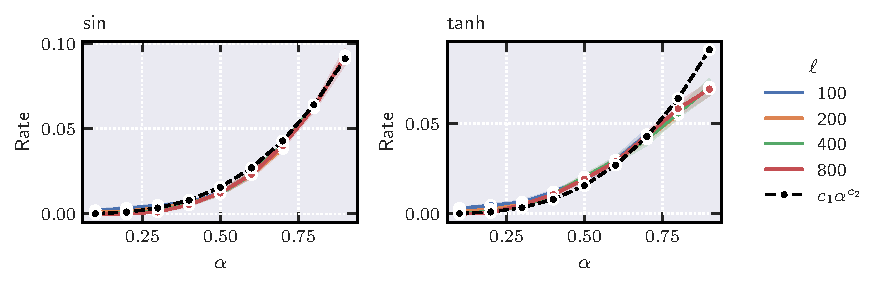
\includegraphics[width=0.8\linewidth]{figures/rate_vs_gain.pdf}
    \caption{Explosion rate of the log norm of the gradients at initialization for an MLP model with
orthogonal weights and batch normalization, for sin and tanh nonlinearities measured for a $1000$
layer deep model at layers $\ell$ as a function of gain $\alpha$. The black trace shows the fitted function $c_1 \alpha^c_2$. Traces are averaged over $10$ independent runs, with the shades showing the $95\%$ confidence interval.}
    \label{grad:fig:rate_vs_gain}
\end{figure}

This reduces the problem to picking the exponent such that the sum stays bounded. We show how the behaviour of the explosion rate at the early layers, for various models, is impacted by the exponent in Figure~\ref{grad:fig:rate_vs_exponent}. Note that for several exponent values, we able to reduce the exponential explosion rate and obtain trainable models, which we show in Section~\ref{grad:sec:other_experiments}.

\begin{figure}[ht]
    \centering
    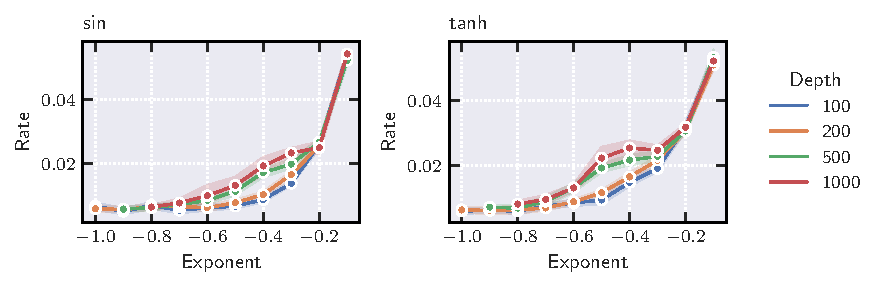
\includegraphics[width=0.8\linewidth]{figures/rate_vs_exponent.pdf}
    \caption{Explosion rate of the log norm of the gradients at initialization for an MLP model with orthogonal weights and batch normalization, for sin and tanh nonlinearities at depths $100, 200, 500, 1000$ as a function of the gain exponent. Traces are averaged over $10$ independent runs, where the shade shows the $95\%$ confidence interval. Rate is measured at $\ell=10$ to avoid the any transient effects of the function}
    \label{grad:fig:rate_vs_exponent}
\end{figure}

\section{Implicit orthogonality during training}
\label{grad:sec:implicity_orthogonality}
In this section, we provide empirical evidence that our architecture during training maintains orthogonality across depths, while maintaining bounded gradients. Figure~\ref{grad:fig:ortho_during_training} shows the evolution of the isometry gap of the weight matrices $W_\ell$ during training, for models at different depths and different nonlinearities. In order to show that these weights are updated gradient descent, we also show the evolution of the norm of the loss gradients with regards to matrices $W_\ell$ in Figure~\ref{grad:fig:gradient_during_training}. 

These experiments are performed on an MLP with orthogonal weight matrices and batch normalization, with sin and tanh activations. The width is set to $100$, batch size $100$ and learning rate $0.001$. The gain exponent is set to a fixed value for all experiments. The measurements are performed on a single batch of size $100$ from CIFAR10, after each epoch of training on the same dataset. 

\begin{figure}[htp!]
    \centering
    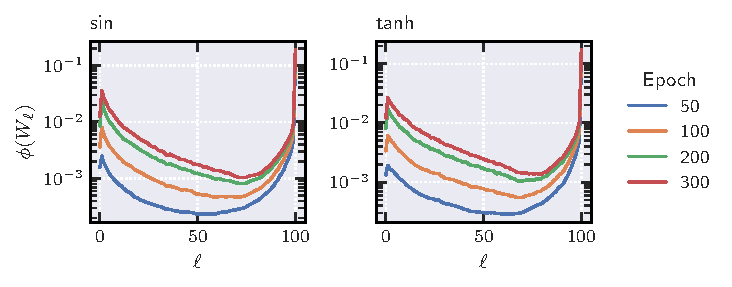
\includegraphics[width=0.8\linewidth]{figures/weight_isogap_during_training_100.pdf}
    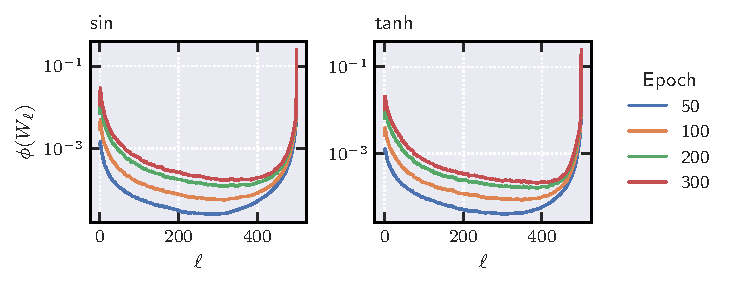
\includegraphics[width=0.8\linewidth]{figures/weight_isogap_during_training_500.pdf}
    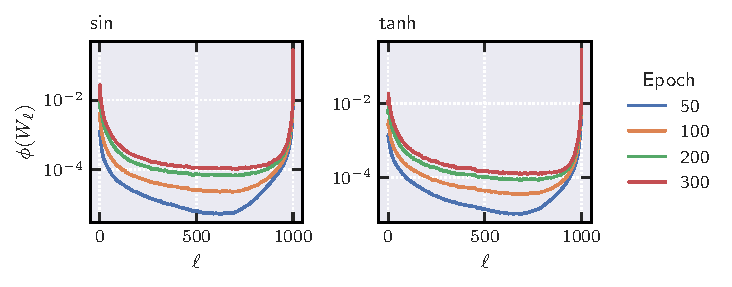
\includegraphics[width=0.8\linewidth]{figures/weight_isogap_during_training_1000.pdf}
    \caption{Contrasting the isometry gap of weight matrices during training for MLPs of depth $100$ (top), $500$ (middle), $1000$ (bottom). The middle layers become increasingly more orthogonal with depth, while maintaining a small isometry gap. During training, the isometry gap also remains low, suggesting the matrices remain close to being orthogonal.}
    \label{grad:fig:ortho_during_training}
\end{figure}

\begin{figure}[htp!]
    \centering
    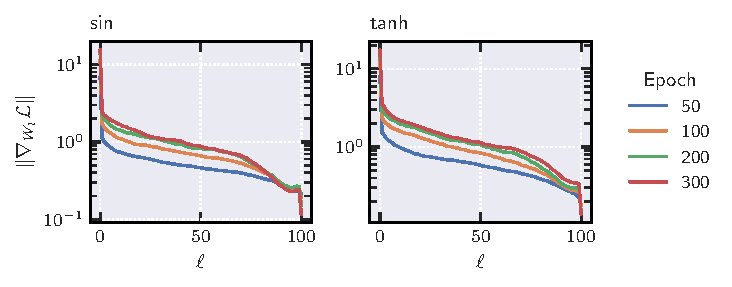
\includegraphics[width=0.8\linewidth]{figures/gradient_during_training_100.pdf}
    \includegraphics[width=0.8\linewidth]{figures/gradient_during_training_500.pdf}
    \includegraphics[width=0.8\linewidth]{figures/gradient_during_training_1000.pdf}
    \caption{Contrasting the Frobenius norm of the gradients of the loss with respect to the weights during training for MLPs of depth $100$ (top), $500$ (middle), $1000$ (bottom). The gradients do not vanish during training and across different depths for all layers, suggesting that the orthogonality evidenced in Figure~\ref{grad:fig:ortho_during_training} is not due to the weights not being updated during SGD.}
    \label{grad:fig:gradient_during_training}
\end{figure}


\section{Other experiments}
\label{grad:sec:other_experiments}
In this section we provide the train and test accuracies of deep MLPs on 4 popular image datasets, namely MNIST, FashionMNIST, CIFAR10, CIFAR100. Hyperparameters and measurements procedure are described in Section~\ref{grad:sec:experiments}.

\subsection*{Supplementary train and test results on MNIST, FashionMNIST, CIFAR10, CIFAR100}

\begin{figure}[ht]
    \centering
    \includegraphics[width=1.0\linewidth]{figures/train_MNIST.pdf}
    \includegraphics[width=1.0\linewidth]{figures/test_MNIST.pdf}
    \caption{Contrasting the train and test accuracy of MLPs with gained sin, tanh and identity activations on MNIST. The identity activation performs much worse than the nonlinearities, indicating the fact that the sin and tanh networks are not operating in the linear regime. The network is trained with vanilla SGD and the hyperparameters are width $100$, batch size $100$, learning rate $0.001$.}
    \label{grad:fig:mnist}
\end{figure}

\begin{figure}[ht]
    \centering
    \includegraphics[width=1.0\linewidth]{figures/train_FashionMNIST.pdf}
    \includegraphics[width=1.0\linewidth]{figures/test_FashionMNIST.pdf}
    \caption{Contrasting the train and test accuracy of MLPs with gained sin, tanh and identity activations on FashionMNIST. The identity activation performs much worse than the nonlinearities, indicating the fact that the sin and tanh networks are not operating in the linear regime. The networks are trained with vanilla SGD and the hyperparameters are width $100$, batch size $100$, learning rate $0.001$.}
    \label{grad:fig:fashionmnist}
\end{figure}

\begin{figure}[ht]
    \centering
    \includegraphics[width=1.0\linewidth]{figures/train_CIFAR100.pdf}
    \includegraphics[width=1.0\linewidth]{figures/test_CIFAR100.pdf}
    \caption{Contrasting the train and test accuracy of MLPs with gained sin, tanh and identity activations on CIFAR100. The identity activation performs much worse than the nonlinearities, indicating the fact that the sin and tanh networks are not operating in the linear regime. The networks are trained with vanilla SGD and the hyperparameters are width $100$, batch size $100$, learning rate $0.001$.}
    \label{grad:fig:cifar100}
\end{figure}

\begin{figure}[ht]
    \centering
    \includegraphics[width=1.0\linewidth]{figures/test_CIFAR10.pdf}
    \caption{Contrasting the train test accuracy of MLPs with gained sin, tanh and identity activations on CIFAR10. The identity activation performs much worse than the nonlinearities, indicating the fact that the sin and tanh networks are not operating in the linear regime. The networks are trained with vanilla SGD and the hyperparameters are width $100$, batch size $100$, learning rate $0.001$.}
    \label{grad:fig:cifar10_test}
\end{figure}

\subsection*{Supplemental figures}
We present empirical results in Figure~\ref{grad:fig:degenerate_input} showing that degenerate input batches are a hard constraint for orthogonalization without gradient explosion. For MLPs with different depths, we show that by repeating samples in a batch of size $10$ we get an exponential gradient explosion, which is unavoidable theoretically.



Furthermore, we show how non-linearities affect the gradient explosion rate in Figure~\ref{grad:fig:nonlinear_contrast}. Using standard batch normalization and fully connected layers from PyTorch we show that non-linearities maintain a large isometry gap. This is a critical issue for our theoretical framework, since we take advantage of the fact that the identity activation achieves perfect orthogonality in order to prove that the gradients remain bounded in depth.
\begin{figure}[ht]
    \centering
    \includegraphics[width=0.9\linewidth]{figures/log_nonlinearities.pdf}
    \vspace{-.4cm}
    \caption{Left: average log-norm of gradients (log-scale y-axis) at the first layer for networks with different depths, evaluted on CIFAR10. Right: Isometry gap (log-scale y-axis) at the last layer for networks with different depths, evaluted on CIFAR10. The MLP is initialized with orthogonal weights and batch normalization, with standard modules, with $\sin, \tanh, \text{identity}$ non-linearities. After stabilizing the isometry gap, the non-linearities have an exponential gradient explosion.
    }
    \label{grad:fig:nonlinear_contrast} 
\end{figure}

\subsection*{Influence of mean reduction on the gradient bound}
In this section, we compare whether adding mean reduction and the additional factor of $\frac1n$ in the denominator of the batch normalization module influences our gradient bound. As expected, we show in Figure~\ref{grad:fig:mean_reduction} that in both cases, for the identity activation, the result remains similar, with the gradients remaining bounded in depth. 
\begin{figure}[ht!]
    \centering
    \includegraphics[width=0.6\linewidth]{figures/log_mean_reduction.pdf}
    \vspace{-.4cm}
    \caption{Comparing the gradient explosion rate in networks with standard batch normalization (blue) and networks with the simplified batch normalization operator from our theoretical framework (orange). Notice that the 2 traces are similar in terms of gradient explosion. Traces are averaged over $10$ runs with the shaded regions showing the $95\%$ confidence interval. Samples are from CIFAR10.
    }
    \label{grad:fig:mean_reduction} 
\end{figure}

% \section{High probability log-gradient bound}
% \begin{theorem}
% In the same conditions as Theorem~\ref{grad:thm:explosion_appendix}, it there is constant $C$ such that:
% $$
% \Pr\Big(\log\|\nabla_{W_\ell}\mathcal{L}\|_{op}\ge  C  \log(1/\delta) d^{6}(\psi(X^0)^3+1)\Big) \le 2\delta 
% $$
% for any $\delta \in(0,1).$
% \end{theorem}

% For example for $\delta=1/2,$ we we have $\|\nabla_{W_\ell}\mathcal{L}\|_{op}\lesssim d^{6}(\psi(X^0)^3+1)$ with at most $1/2$ probability. 
% \begin{proof}
% We follow the same proof as Theorem~\ref{grad:thm:explosion_appendix} by decomposing the log gradient to sum of log gradients of each layer. Note that Lemma~\ref{grad:lem:jacobian_bn_norm} holds deterministically, as it is valid by construction. Thus, what remains is to derive a probabilistic version of Lemma~\ref{grad:lem:jacobian_log_norm_bound}. We start from \eqref{grad:eqn:op_bound} which holds deterministically, to arrive at a probabilistic bound:
% \begin{align}
% \sum_{k = 1}^L \log \norm{J_{\BN}(H^k)} \le S (d\psi(X^0)) + 2\sum_{\ell=S+1}^L \sqrt{d\psi(X^\ell)}, \qquad S:= \min\left\{\ell: \psi(X^\ell)\le \frac{1}{16d^2}\right\}
% \end{align}
% We derive a probabilistic bound for each term.
% \newcommand{\Event}{\mathcal{E}}
% \paragraph{First term.}
% Based on Lemma~\ref{grad:lem:hitting_layer} we have $E [S] \lesssim d^4 \psi(X^0)^2.$ Thus, there is $C_0$ such that $$\exists C_0: E [S] \le \frac{C_0}{2} d^4 \psi(X^0)^2 .$$ Thus, by Markov inequality we have 
% $$P (S\ge B) \le \frac{\E[S]}{B } \le \frac12, \qquad B:=  C_0 d^4 \psi(X^0)^2. $$ 

% First, we discretize the layers into blocks of size $B$, where $B$ is defined above. With a slight abuse of notation, define $B_i$ as the end of the $i$th block of size $B$, and let $E_i$ be the event $E_i = \{\psi(X_{B_i}) > \frac{1}{16d^2}\}$, which is the event of failure for $\psi$ to drop below the threshold of $\frac{1}{16d^2}$ after the last layer from block $i$.

% By the inequality established above, we know that in each block, $\psi$ can either fall below the threshold, or stay above, with probability at most $1/2$. Moreover, knowing that $\psi$ is non-increasing, we know that $P(E_i | E_{<i}) \leq 1/2$.

% Thus, by the non-increasing property of $\psi$, the probability of failure after $k$ blocks of size $B$ is at most the probability that $\psi$ did not fall below the threshold in any of the $k$ successive blocks:

% \begin{align}
%     P(E_k) &\leq P(E_1 \wedge \dots \wedge E_{k-1}) \\
%     &= P(E_1) P(E_2 | E_1) \dots P(E_{k} | E_{k-1} \dots E_1) \\
%     &\leq \left(\frac{1}{2}\right)^k
% \end{align}

% Thus, we obtain the probability:
% \begin{align}
%     P(S \geq kB) = P(S \geq k C_0 d^4 \psi(X_0)^2) \leq 2^{-k}
% \end{align}

% Thus, connecting back to gradients, we obtain:
% \begin{align}
%     \Pr\Big(\sum_{\ell=0}^S \|J_{\BN}(H^\ell)\|_{op} \ge k C_0 d^5 \psi(X^0)^3 \Big)\le 2^{-k}.
% \end{align}

% \paragraph{Second term} Starting from~\eqref{grad:eqn:after_thresh}, we have 
% $$
% \ell \ge S \implies \Pr\Big\{\psi(X^{\ell+1})\ge (1-1/4d^2)\psi(X^\ell)\Big\} \le 1- \frac{1}{4d^2}
% $$
% Let $E_\ell$ denote the event that $\psi(X^{\ell+1})$ does not decrease by $1-1/4d^2$ compared to its previous layer:
% $E_\ell = \1\Big\{\psi(X^{\ell+1})\ge (1-1/4d^2)\psi(X^\ell)\Big\}.$
% Due to the non-increasing property of $\psi$, we know that $\Pr(E_\ell) = \Pr(E_\ell | E_{\ell-1})$. Repeating this for $s$ steps, we obtain:

% \begin{align}
%     \ell \ge S \implies \Pr\Big\{\psi(X^{\ell+s})\ge (1-1/4d^2)\psi(X^\ell)\Big\} =
%     \prod_{i=\ell}^{\ell+s-1} \Pr\{ E_{i+1} | \bar E_{i} \} \leq (1 - \frac{1}{4d^2})^s
% \end{align}

% Inspired by this, consider the sequence $\ell_0, \ell_1, \dots$ defined as 
% $$
% \ell_0 = S, \qquad \ell_{k} = \ell_{k-1} + 4 c k d^2
% $$
% Thus, we get:
% $$
% \Pr\Big\{\psi(X^{\ell_{k+1}})\ge (1-\frac{1}{4d^2})\psi(X^{\ell_{k}})\Big\} \le (1- \frac{1}{4d^2})^{4 c k d^2} \le e^{-ck}
% $$
% Thus, we have the union bound 
% \begin{align*}
% \Pr\Big\{\bigvee_{k=0}^\infty \psi(X^{\ell_{k+1}})\ge (1-\frac{1}{4d^2})\psi(X^{\ell_k}) \Big\} \le \sum_{k=1}^\infty e^{-ck} = \frac{e^{-c}}{1-e^{-c}}\\
% \implies \Pr\Big\{\underbrace{\bigwedge_{k=0}^\infty \psi(X^{\ell_{k+1}})\le (1-\frac{1}{4d^2})\psi(X^{\ell_k}) }_{Q:=}\Big\} \ge 1- \frac{e^{-c}}{1-e^{-c}}= \frac{1-2e^{-c}}{1-e^{-c}}
% \end{align*}
% Note that in the event that $Q$ holds, we can the isometry gaps in each $[\ell_{k-1},\ell_k]$ interval as:
% $$
% Q \implies \psi(X_\ell) \le \frac{1}{16d}(1-\frac{1}{4d^2})^{k-1} \text{ for all } \ell \in [\ell_{k-1},\ell_{k})
% $$
% We can upper bound $\sum_{\ell=S+1}^\infty \sqrt{d \psi(X^\ell)}$ by using the numbers of items and upper bound on each block. Thus, assuming for all $k$  we have  $\psi(X^{\ell_{k+1}})\le (1-\frac{1}{4d^2})\psi(X^{\ell_k}),$ we can derive
% \begin{align*}
% Q \implies \sum_{\ell=S+1}^\infty \sqrt{d\psi(X_\ell)} &\le \sum_{k=1}^\infty (\ell_{k}-\ell_{k-1})\sqrt{d \frac{1}{16d} (1-\frac{1}{4d^2})^{k}}\\
% & = cd^2 \sum_{k=1}^\infty k (1-\frac{1}{4d^2})^{k/2} \\
% &\le c d^2 \sum_{k=1}^\infty k(1-\frac{1}{8d^2})^k && \text{using $(1+x)^{1/2}\le 1+x/2$}\\
% &= cd^2 \frac{1-8/d^2}{(1/8d^2)^2}   && \text{using $\sum_{k=1}^\infty k\alpha^k = \alpha/(1-\alpha)^2.$}\\
% &\le 64 c d^6 
% \end{align*}
% Thus we have:
% $$
% \Pr\left(\sum_{\ell=S+1}^\infty \sqrt{d\psi(X_\ell)} \le 64 c d^6 \right) \ge \Pr\Big\{Q \Big\} \ge \frac{1-2e^{-c}}{1-e^{-c}}
% $$
% which yields 
% $$
% \Pr\left(\sum_{\ell=S+1}^\infty \log\|J_{BN}(H^\ell)\|_{op}  \ge 64 c d^6 \right) \le \Pr(\overline Q)= \frac{e^{-c}}{1-e^{-c}}
% $$
% Combining first and second term bounds for the Jacobian log-norms we have
% \begin{align}
% \Pr\Big(\sum_{l=\ell}^S \log\|J_{\BN}(H^l)\|_{op} > k C_0 d^5\psi(X^0)^3\Big) &\le 2^{-k} \\
% P\left(\sum_{\ell=S+1}^\infty \log\|J_{\BN}(H^l)\|_{op} \ge 64 cd^{6}\right) &\le \frac{e^{-c}}{1-e^{-c}}
% \end{align}
% And thus we have 
% $$
% \Pr\Big(\sum_{l=\ell}^L\log\|J_{BN}(H^l)\|_{op} \ge k C_0 d^5\psi(X^0)^3 + 64 cd^{6}\Big) \le 2^{-k} + \frac{e^{-c}}{1-e^{-c}}
% $$
% Thus, we can find $C$ such that 
% $$
% \Pr\Big(\log\|\nabla_{W_\ell}\mathcal{L}\|_{op}\ge k C  d^{6}(\psi(X^0)^3+1)\Big) \le 2^{-k+1}
% $$
% We can finish the proof by defining $\delta = 2^{-k}$ and change of variables $k = \log(1/\delta).$
% \end{proof}

% \section{Gradients in Residual networks}
% \begin{figure}[htp]
%     \centering
%     \includegraphics{figures/rebuttal_residual.pdf}
%     \caption{Logarithmic plot for the gradient norm of the first layer for residual networks with batch normalization initialized with Gaussian weights at different depths, evaluated on CIFAR10. The traces show that the gradients do not remain bounded in depth for different activations.}
%     \label{grad:fig:residuals}
% \end{figure}




%%%%%%%%%%%%%%%%%%%%%%%%%%%%%%%%%%%%%%%%%%
%% LIST OF TABLES / FIGURES / ALGORITHMS %
%%%%%%%%%%%%%%%%%%%%%%%%%%%%%%%%%%%%%%%%%%
\pdfbookmark[-1]{Lists of Tables}{lot}
\listoftables{}
\cleardoublepageempty{}
% \listsubcaptions
\pdfbookmark[-1]{Lists of Figures}{lof}
\listoffigures{}
\cleardoublepageempty{}
\pdfbookmark[-1]{Lists of Algorithms}{loa}
\listofalgorithms{}
\cleardoublepageempty{}


%%%%%%%%%%%%%%%%
%% BIBLIOGRAPHY %
%%%%%%%%%%%%%%%%%
\pdfbookmark[-1]{Bibliography}{book:bibliography}
\printbibliography{}
\cleardoublepageempty{}
\clearpage
\cleardoublepageempty{}
\end{document}
